%%%%%%%%%%%%%%%%%%%%%%%%%%%%%%%%%%%%%%%%%
% kaobook
% LaTeX Template
% Version 1.3 (December 9, 2021)
%
% This template originates from:
% https://www.LaTeXTemplates.com
%
% For the latest template development version and to make contributions:
% https://github.com/fmarotta/kaobook
%
% Authors:
% Federico Marotta (federicomarotta@mail.com)
% Based on the doctoral thesis of Ken Arroyo Ohori (https://3d.bk.tudelft.nl/ken/en)
% and on the Tufte-LaTeX class.
% Modified for LaTeX Templates by Vel (vel@latextemplates.com)
%
% License:
% CC0 1.0 Universal (see included MANIFEST.md file)
%
%%%%%%%%%%%%%%%%%%%%%%%%%%%%%%%%%%%%%%%%%

%----------------------------------------------------------------------------------------
%	PACKAGES AND OTHER DOCUMENT CONFIGURATIONS
%----------------------------------------------------------------------------------------

\documentclass[
	a4paper, % Page size
	fontsize=10pt, % Base font size
	twoside=true, % Use different layouts for even and odd pages (in particular, if twoside=true, the margin column will be always on the outside)
	%open=any, % If twoside=true, uncomment this to force new chapters to start on any page, not only on right (odd) pages
	%chapterentrydots=true, % Uncomment to output dots from the chapter name to the page number in the table of contents
	numbers=noenddot, % Comment to output dots after chapter numbers; the most common values for this option are: enddot, noenddot and auto (see the KOMAScript documentation for an in-depth explanation)
]{kaobook}

% Choose the language
\ifxetexorluatex
	\usepackage{polyglossia}
	\setmainlanguage{english}
\else
	\usepackage[english]{babel} % Load characters and hyphenation
\fi
\usepackage[english=british]{csquotes}	% English quotes

% Load packages for testing
\usepackage{blindtext}
%\usepackage{showframe} % Uncomment to show boxes around the text area, margin, header and footer
%\usepackage{showlabels} % Uncomment to output the content of \label commands to the document where they are used

% Load the bibliography package
\usepackage{kaobiblio}
\addbibresource{./references/bibliography_for_core_thesis.bib} % Bibliography file
\addbibresource{./references/logging_paper.bib} % Bibliography file
% \addbibresource{./references/bibliography_on_phd_experience}

% Load mathematical packages for theorems and related environments
\usepackage[framed=true]{kaotheorems}

% Load the package for hyperreferences
\usepackage{kaorefs}

\graphicspath{{examples/documentation/images/}{images/}} % Paths in which to look for images

\makeindex[columns=3, title=Alphabetical Index, intoc] % Make LaTeX produce the files required to compile the index

\makeglossaries % Make LaTeX produce the files required to compile the glossary
\section{Glossary with Abbreviations}
\label{the-glossary}
\newcounter{headercounter}
\newcommand{\boxedheader}[1]{%
  \stepcounter{headercounter}%
  \begin{tikzpicture}[remember picture]
  \path[thick,rounded corners=1mm,draw=gray,fill=gray!40!white,overlay]
    (-0.2,-0.25\baselineskip) rectangle ([xshift=2mm,yshift=0.75\baselineskip]pic cs:tableright\roman{headercounter});
  \end{tikzpicture}%
  #1
  \tikzmark{tableright\roman{headercounter}}\\%
}

\begin{comment}
% This is hidden as it is a hack that doesn't work well however it does set the heading box to full width unlike the one below. However I've spent far more time on this than it justifies at this stage.

\newtcolorbox{mybox}[1][]{%
    enhanced jigsaw,
    boxrule=0.5pt,
    left=0pt,right=0pt,top=0mm,bottom=0mm, 
    colback = gray!20,
    height=2cm,
    arc=1mm,
}

\newcolumntype{R}{>{\raggedleft\arraybackslash}p{1cm}}
\newcolumntype{C}[1]{>{\centering\arraybackslash}p{#1}}

\begin{mybox}
\begin{longtabu} to \linewidth {@{\,}XZ@{}}
    \textbf{Term}  & \textbf{Description and remarks} 
\end{longtabu}%
\end{mybox}%
\end{comment}

\newcolumntype{Z}{>{\raggedright\arraybackslash}p{10cm}}

\begin{longtabu} to \linewidth {@{\,}X[1]Z@{}} %\linewidth {@{}Xcr@{}}
\boxedheader{\textbf{Term} & \textbf{Description and remarks} \extracolsep{\fill} } \\
Analogue Feedback & Here, used to identify feedback from human sources. Generally this feedback is intentional \emph{i.e.} the person chooses to provide the feedback. The feedback may vary massively from one instance to another. \\

Android Vitals~\label{glossary_android_vitals} & \\

ANR & Abbreviation for \emph{Application Not Responding}. \\

API &Application Programming Interface. \\
Application~\mbox{Not Responding} & A term originated by Google to identify when an Android app stops responding to users for over 5 seconds~\citep{google_play_view_crashes_and_ANR_errors}. \\

Crash Analytics &Analysis of application crashes collected automatically by software. Identify groupings and patterns in the crashes to provide developers with the opportunity to debug and fix them without needing to spend time reproducing the problem. (Paraphrased from~\citep{ibm_mobile_foundation_7_1_app_crash_analytics}. \\

Developer account & For the purposes of this research we use Google's concept of a Google Play Developer Account, described variously in~\cite{google_play_how_to_use_the_play_console, google_play_launch_checklist}. Developers need to register for an account, pay a one-time fee, and agree to abide by various policies, terms, and conditions. Someone who has a developer account can invite other people to share aspects of their account. \\

Digital Feedback & Here used to identify feedback from running software, generated automatically. The feedback is structured and the structure generally consistent. \\
Google Play Console & A Web-based application which is the primary user interface for developers who release Android apps in the Google Play Store. Google also provides mobile apps that provide a subset of the capbabilities of Google Play Console. \\

Error & ``An \textbf{error} is a system state that may cause a failure."~\citep{abreu2007_on_the_accuracy_of_spectrum_based_fault_localization}, based on~\citep{avizienis2004_basic_concepts_and_taxonomy}.\\

EULA & End User License Agreement. \\

Event demographics & \emph{`Percentage of events triggered by each age group and gender.'} (Source: Google Firebase Analytics tooltip).\\

Explicit Feedback &For example, in the form of reviews and comments~\citep{maalej2016_towards_data_driven_requirements_engineering}. \\

Failure & ``A \textbf{failure} is an event that occurs when delivered service deviates from correct service. "~\citep{abreu2007_on_the_accuracy_of_spectrum_based_fault_localization}, based on~\citep{avizienis2004_basic_concepts_and_taxonomy}.\\

Failure Repositories &A central location in which data pertaining to failures of software is stored and managed. Notes: Definition based on a service, ~\href{https://languages.oup.com/google-dictionary-en/}{Oxford Languages}, jointly provided by Google and Oxford University Press. Mentioned but not defined in various sources including:~\citep{maalej2016_towards_data_driven_requirements_engineering}, and exemplified in~\citep{cfdr_usenix}.\\

Fault & ``A fault is the cause of an error in the system."~\citep{abreu2007_on_the_accuracy_of_spectrum_based_fault_localization}, based on~\citep{avizienis2004_basic_concepts_and_taxonomy}.\\

FunDex & A score devised by Hewlett-Packard (HP) as part of their AppPulse Mobile product offering. \emph{``The score starts at 100, but drops with each problem the app has ..."}~\citep{hall2015_HP_courts_developers_with_tools_for_monitoring_mobile_apps}. It combines scores for UI performance, stability, and resource usage. \\

GDPR &\href{https://gdpr-info.eu/}{General Data Protection Regulation}.\\ 

Implicit Feedback &Automatically collected information about software usage~\citep{maalej2016_towards_data_driven_requirements_engineering}.\\

Interaction screen &Interaction screen conveys the screen as both an output and input device (rather than the term touch screen)~\footnote{This term is originated by Prof. Arosha K. Bandara, thank you.}. \\

JVM~\label{glossary_jvm} & Java Virtual Machine, for the purposed of this thesis the JVM runs Android apps written in Java and Kotlin. It is not used to run \href{glossary_native_code}{native code}. \\

Mobile App Analytics Tools & ``Mobile app analytics tools collect and report on in-app data pertaining to the operation of the mobile app and the behavior of users within the app, as well as aggregate market data on apps across public app stores"~\citep{gartner2015_market_guide_for_mobile_app_analytics}. \\

Operational Analytics & ``Operational analytics: Provides visibility into the availability and performance of mobile apps in relation to device, network, server and other technology factors. Operational analytics are essential to capture and fix unexpected app behavior (such as crashes, bugs, errors and latency) that can lead to user frustration and abandonment of the app."~\citep{gartner_what_is_mobile_app_analytics_software} \\

PII &Personally Identifiable Information. \emph{``Personally Identifiable Information; Any representation of information that permits the identity of an individual to whom the information applies to be reasonably inferred by either direct or indirect means."}~\citep{nist_pii}\\ 

Platform &Here, a platform includes an operating system, related software resources (including APIs and services), and an ecosystem including an app store. Google Android and Apple's iOS are both mobile platforms. They run on end-user devices and capture aspects of the software that runs on those devices. Platform services can monitor apps from the time they are installed until they are removed. \\

Mobile Analytics Policy~\label{glossary-mobile-analytics-policy} &Defines the `rules of engagement' when incorporating mobile analytics as part of the development, maintenance and where appropriate the operation of a mobile app. \\

Mobile Analytics Strategy~\label{glossary-mobile-analytics-strategy} &Describes how the team intend to work within their mobile analytics policy to achieve the aims and objectives of using mobile analytics. \\

OBB~\label{glossary-obb-file-format} &Android Opaque Binary Blob File~\citep{fileinfo_obb_format}, used to package expansion files for Android APK files~\citep{apk_expansion_files}. \\

Native Code~\label{glossary_native_code} &Written in C++ and native to the computer (device) architecture. \\

QoE & Abbreviation for \emph{Quality of Experience}. \\

Quality of Experience & Oft used in Mobile Telecommunications to measure network transmission characteristics. Here used so we can more easily identify and consider the quality of experiences such as \emph{User Experience}. TBD whether to focus on perceived experience as perceived by end users of an app. \\

Risk & ``A risk is an unwanted event that has negative consequences."~\citep{pfleeger2000_risky_business} \\

Service Provider &An organisation, often commercial, which includes software, and online services (and the people who provide these) that offers developers optional facilities such as in-app- analytics, crash reporting, messaging, feedback mechanisms, \emph{etc.} \\

Stability &A software quality identified initially by HP as part of their FunDex~\citep{calleosoftware_AppPulseMobile}. The same term was subsequently used by Google to identify and measure two related indications of software failures: crashes and freezes. \\ %SHOULD_DO add references to cite both sources. 

~\href{section-vitals-scraper}{\emph{Vitals Scraper}} &Opensource software developed as part of this research to facilitate the downloading, analysis, and preservation of various reports in Google Play Console and Android Vitals. \\

UX & Abbreviation for User Experience. \\

\caption{Glossary with Abbreviations} \\
\end{longtabu}


%\end{table}

% Thanks to https://tex.stackexchange.com/questions/503784/how-to-arrange-tabular-in-alphabetical-order for the table formatting.
% and to get it to fit on a page https://tex.stackexchange.com/questions/27097/changing-the-font-size-in-a-table
% And the following to help me stop "Application Not Responding" from being split mid-word: https://texfaq.org/FAQ-wdnohyph
% https://tex.stackexchange.com/questions/121832/breaking-words-at-the-end-of-line/121835
%  https://tex.stackexchange.com/questions/380613/hyphenat-not-hyphenating-words-with-hyphens

% Replaced the previous structure with longtabu, a package that's caused some furore in the TeX community to enable the glossary to run to several pages
% https://tex.stackexchange.com/questions/201419/longtabu-rounded-box-in-the-header provided the main example
% I reached the above from https://tex.stackexchange.com/questions/201387/how-to-combine-mdframed-and-tabu however I abandoned the mdframed eventually as my table was longer than a page.
% https://sites.google.com/site/simonthelwall/home/latex provided some useful additional notes and has lots of other useful examples, including working with citations and tufte document templates.

% Possible alternatives
% If I can get my head around the following:
% https://tex.stackexchange.com/questions/501097/split-table-on-two-pages 

% Or try applying the following which will add column headings
% https://tex.stackexchange.com/a/456976/88466 

\clearpage % Include the glossary definitions

\makenomenclature % Make LaTeX produce the files required to compile the nomenclature

% Reset sidenote counter at chapters
%\counterwithin*{sidenote}{chapter}

%----------------------------------------------------------------------------------------
%	CUSTOM CODE FROM JULIAN
%----------------------------------------------------------------------------------------

\newskip\tufteskipamount
\tufteskipamount=1.0\baselineskip plus 0.5ex minus 0.2ex

\newcommand{\tuftebreak}{\par\ifdim\lastskip<\tufteskipamount
  \removelastskip\penalty-100\tufteskip\fi}

\newcommand{\tufteskip}{\vspace\tufteskipamount}

\makeatletter
\def\tuftebreak{%
  \if@nobreak\else
    \par
    \ifdim\lastskip<\tufteskipamount
      \removelastskip \penalty -100
      \tufteskip
    \fi
  \fi
}
\makeatother

%--------------------------------------------

\newlength\ltempa
\newlength\ltempb
\newcommand\newthought[1]{%
   %\addvspace{1.0\baselineskip plus 0.5ex minus 0.2ex}%
   \noindent\expandafter\formatnewthought#1\relax}
\def\formatnewthought#1#2\relax{%
  \tuftebreak
  \settowidth\ltempa{\textsc{#1#2}}%
  \settowidth\ltempb{\textsc{#1\mbox{}#2}}%
  \addtolength\ltempa{-\ltempb}%
  \textbf{#1}\kern\ltempa\textsc{#2}%
}

%--------------------------------------------
%\usepackage[anythingbreaks]{breakurl}
\usepackage{etoolbox}
\appto\UrlBreaks{\do\-}

\usepackage{comment}
\usepackage{nth}
\usepackage{copyrightbox}
\usepackage{svg}
\usepackage{subfig}
\usepackage[normalem]{ulem}
\usepackage{cancel}  % https://jansoehlke.com/2010/06/strikethrough-in-latex/
\useunder{\uline}{\ul}{}

\setminted{fontsize=\small,baselinestretch=1}  % shrink code samples so they don't overwhelm the text.
%--------------------------------------------

\newcommand{\secref}[1]{\autoref{#1}. \nameref{#1}} % \secref{section:my} %from https://stackoverflow.com/a/30844515/340175

%--------------------------------------------

% comment these for final
\newcommand{\yijun}[1]{\textcolor{red}{[YY: #1 ?]}}
% \def\yy#1#2{\textcolor{red}{#1}\footnote{YY:{#2}\textcolor{black}}}
\newcommand{\yy}[2]{{#1}\footnote{YY:{#2}}}

\newcommand{\akb}[1]{\textcolor{purple}{[AKB: #1]}}
\newcommand{\arosha}[1]{\textcolor{purple}{[AKB: #1 ?]}}

\newcommand{\marian}[1]{\textcolor{blue}{[MP: #1 ?]}}
\newcommand{\julian}[1]{\textcolor{olive}{[JH: #1]}}
\newcommand{\isabel}[1]{\textcolor{brown}{[IE: #1]}}


%--------------------------------------------

% To address the error: Class scrbook Error: undefined old font command `\sf'.
% From: https://github.com/ftilmann/latexdiff/issues/92 
\makeatletter
\DeclareOldFontCommand{\rm}{\normalfont\rmfamily}{\mathrm}
\DeclareOldFontCommand{\sf}{\normalfont\sffamily}{\mathsf}
\DeclareOldFontCommand{\tt}{\normalfont\ttfamily}{\mathtt}
\DeclareOldFontCommand{\bf}{\normalfont\bfseries}{\mathbf}
\DeclareOldFontCommand{\it}{\normalfont\itshape}{\mathit}
\DeclareOldFontCommand{\sl}{\normalfont\slshape}{\@nomath\sl}
\DeclareOldFontCommand{\sc}{\normalfont\scshape}{\@nomath\sc}
\makeatother

%----------------------------------------------------------------------------------------
% From https://tex.stackexchange.com/a/330980/88466
% It fixes several compilation warnings about having \\ to split the title of the thesis, etc.

\pdfstringdefDisableCommands{%
  \def\\{}%
  \def\texttt#1{<#1>}%
}

%----------------------------------------------------------------------------------------
% The following clashes with the \requirepackage{todonotes} which is part of kaobook
%\usepackage[colorinlistoftodos,prependcaption,textsize=tiny]{todonotes}  % From https://tex.stackexchange.com/a/178806/88466

\begin{comment}
\newcommandx{\unsure}[2][1=]{\todo[linecolor=red,backgroundcolor=red!25,bordercolor=red,#1]{#2}}
\newcommandx{\change}[2][1=]{\todo[linecolor=blue,backgroundcolor=blue!25,bordercolor=blue,#1]{#2}}
\newcommandx{\pending}[2][1=]{\todo[linecolor=OliveGreen,backgroundcolor=OliveGreen!25,bordercolor=OliveGreen,#1]{#2}}
\newcommandx{\improvement}[2][1=]{\todo[linecolor=Plum,backgroundcolor=Plum!25,bordercolor=Plum,#1]{#2}}
\newcommandx{\thiswillnotshow}[2][1=]{\todo[disable,#1]{#2}}
\end{comment}

%----------------------------------------------------------------------------------------
% Adjustbox is used to shrink a couple of large tables. I'd like to find a better approach, however it does an adequate job.

\usepackage{adjustbox}

%----------------------------------------------------------------------------------------
% Limit the per chapter mini table of contents to showing sections, not subsections.
\setcounter{margintocdepth}{\sectiontocdepth}

%----------------------------------------------------------------------------------------
\usepackage{array,tabularx,longtable,tabu}
\newcolumntype{R}[1]{>{\raggedleft\arraybackslash}p{#1}} % Define a new right-aligned paragraph column type
\newcolumntype{L}[1]{>{\raggedright\arraybackslash}p{#1}} % Define a new left-aligned (no justification) paragraph column type
\newcolumntype{C}[1]{>{\centering\arraybackslash}p{#1}} % Define a new centered paragraph column type


%----------------------------------------------------------------------------------------
\usepackage{epigraph} % To have quotes at the start of chapters.
\setlength{\epigraphwidth}{0.5\linewidth}
%----------------------------------------------------------------------------------------

%%%%%%% A set of macros for the six perspectives
% Implementation inspired by https://newbedev.com/how-to-change-dot-spacing-in-dotfill

\makeatletter
\newcommand \iuse {I\textsuperscript{use}}
\newcommand \iartefacts {I\textsuperscript{artefacts}}
\newcommand \itools {I\textsuperscript{tools}}
\newcommand \uuse {U\textsuperscript{use}}
\newcommand \uartefacts {U\textsuperscript{artefacts}}
\newcommand \utools {U\textsuperscript{tools}}
\makeatother 

%----------------------------------------------------------------------------------------
% This quick and dirty approach comes from a comment on https://tex.stackexchange.com/q/191295/88466
% A quick and dirty method is to wrap the text into a command, which both prints your text and the makes an entry to the index: \newcommand{\myindex}[1]{#1\index{#1}}, e.g. \myindex{Einstein} will print Einstein right there and generates the index entry Einstein too. However, this is a cheap 'hack' and will not work for more sophisticated index entries ;-) – user31729  Jul 13, 2014 at 15:15 

% I'll try using it for now, otherwise I can advance to the improved approach in the answer https://tex.stackexchange.com/a/191303/88466

\newcommand{\myindex}[1]{#1\index{#1}}

%----------------------------------------------------------------------------------------

\begin{document}

%----------------------------------------------------------------------------------------
%	BOOK INFORMATION
%----------------------------------------------------------------------------------------

%\titlehead{ORCID \href{https://orcid.org/0000-0003-4052-0054}{0000-0003-4052-0054}}
\subject{PhD Thesis}

\title{Improving Application Quality\\ using Mobile Analytics}
\subtitle{}

\author{\textsc{Julian Harty}\\\small ORCID \href{https://orcid.org/0000-0003-4052-0054}{0000-0003-4052-0054}}

\date{\today}

\publishers{Department of Computing and Communications\\ Faculty of STEM\\ \textsc{The Open University}\\\bigskip\bigskip Supervisors:\\ Arosha Bandara \& Yijun Yu}

%----------------------------------------------------------------------------------------

\frontmatter % Denotes the start of the pre-document content, uses roman numerals

%----------------------------------------------------------------------------------------
%	OPENING PAGE
%----------------------------------------------------------------------------------------

%\makeatletter
%\extratitle{
%	% In the title page, the title is vspaced by 9.5\baselineskip
%	\vspace*{9\baselineskip}
%	\vspace*{\parskip}
%	\begin{center}
%		% In the title page, \huge is set after the komafont for title
%		\usekomafont{title}\huge\@title
%	\end{center}
%}
%\makeatother

%----------------------------------------------------------------------------------------
%	COPYRIGHT PAGE
%----------------------------------------------------------------------------------------

\makeatletter
\uppertitleback{\@titlehead} % Header

\lowertitleback{
	\textbf{Disclaimer}\\
	Errors and Omissions excepted. 
	
	\medskip
	
	% TODO confirm the actual copyright.
	\textbf{Copyright}\\ % The following was created using https://chooser-beta.creativecommons.org/
	\ccbyncndeu\
	Improving Application Quality using Mobile Analytics © 2022 by Julian Harty is licensed under CC BY-NC-ND 4.0.
	
	To view a copy of the CC-BY-NC-ND code, visit: \\\url{http://creativecommons.org/licenses/by-nc-nd/4.0/}
	
	\medskip
	
	\textbf{Colophon} \\
	This document was typeset with the help of \href{https://sourceforge.net/projects/koma-script/}{\KOMAScript} and \href{https://www.latex-project.org/}{\LaTeX} using the \href{https://github.com/fmarotta/kaobook/}{kaobook} class.
	
	The source code of this book is available at:\\\url{https://github.com/fmarotta/kaobook}
	
	(You are welcome to contribute!)
	
	\medskip
	
	\textbf{Publisher} \\
	First printed in July 2022 by \@publishers
}
\makeatother

%----------------------------------------------------------------------------------------
%	DEDICATION
%----------------------------------------------------------------------------------------

\dedication{
	Here goes the dedication. Let’s start with persistence in the face of the many challenges and the help and support of many people who encouraged and guided me as the many challenges of life and research emerged.
	
	\bigskip % Vertical whitespace
	
	The many failures also shaped the research and the learnings through the PhD journey. I have about as many abandoned and rejected papers as those which were accepted.
	
	\bigskip % Vertical whitespace
	
	This work was inspired through my work with real-world developers of very success- ful mobile apps through the early and juvenile years of mobile app development (from 2006 to 2013) where I learned of the power and potential of using mobile analytics to improve the software and how teams create, test and support that software.
	
	\bigskip % Vertical whitespace
	
	To Sheep Dalton who was my co-supervisor at the start and until I completed the probation report, he provided rich and fresh ideas and insights as I was shaping my research.
	
	\bigskip % Vertical whitespace
	
	There’s more to add before this thesis is complete. For now, this will do.
}

%----------------------------------------------------------------------------------------
%	OUTPUT TITLE PAGE AND PREVIOUS
%----------------------------------------------------------------------------------------

% Note that \maketitle outputs the pages before here

\maketitle

%----------------------------------------------------------------------------------------
%	ABSTRACT
%----------------------------------------------------------------------------------------

\chapter*{Abstract}
\addcontentsline{toc}{chapter}{Abstract} % Add the abstract to the table of contents as a chapter

The purpose of this research is to investigate and report on how mobile analytics can help
real-world developers improve the quality of their apps efficiently and effectively. The research also considers the effects of mobile analytics in terms of the artefacts developed and maintained by the development team and also researches key characteristics of a range of mobile analytics tools and services. %The success of their apps may depend, at least in part, on how their apps are rated using externally determined metrics established by an app store.

Research Design: the research takes a developer-oriented perspective of using three complementary sources of data: 1) platform-level analytics, using \myindex{Android Vitals} as the primary analytics tool, 2) in-app analytics with a focus on runtime failures caused by crashes and freezes (known as \Gls{anr} in Android), and 3) interviews with developers.
%
Action research techniques included roles of embedded developer, guide, and observer across different mobile app projects I was involved in. \myindex{Hackathons} were used to experiment with the speed and ability to find and address issues reported by the analytics tools used by the app developers. 
%
Their apps have a combined active user base of over 3,000,000 users. Many of these apps use a mainstream crash analytics library which was used to complement and contrast the results provided in the primary analytics tool.
%
The research is intended to facilitate ease of future research and reproducibility,~\emph{e.g.} by using  open-source\index{Opensource} projects as the code, bug reports, \emph{etc.} are all published and available. This research was complemented by a) collaborating with professional developers who provided additional examples and results, and b) investigating grey material including grey literature and grey data.

The findings of this research highlights that using mobile analytics helped to reduce failure rates markedly, quickly, and effectively by applying techniques described here.
Various limitations and flaws were found in the analytics tools; these provide cause for concern as they may affect the app's placement in the app store and revenues. These limitations and flaws also make some issues in the apps harder to identify, prioritise, and fix. We identified ways to compensate for many of these and developed open-source software to facilitate additional analysis. Flaws and bugs were reported to the Android Vitals team at Google who acknowledged they would fix several of them.
%
Several bugs were hard to reproduce, partly as Google deliberately hid pertinent details from the data they gather. Nonetheless app developers were able to ameliorate or fix the bugs for some issues even when they were not able to reproduce them. 

Android Vitals shows the potential of how the combination of an app store and platform could be used to improve the quality of apps without users needing to actively participate. Some crashes were hard to reproduce and may be impractical to find before the app is released to end users. Developers can determine comparative improvements in their releases, such as whether they fixed a bug, by using Android Vitals and similar analytics tools; \emph{i.e.} mobile analytics may help teams to determine whether they have improved the quality of their app \emph{even with flaws and limitations in the mobile analytics}.


% Improving Application Quality using Mobile Analytics

%% A Good Abstract succinctly answers these four topics:
%% \begin{itemize}
%%    \item What was the purpose of your research?
%%    \item How was your research designed?
%%    \item What were your findings?
%%    \item What were your conclusions?
%% \end{itemize}

%%% Feedback from Yijun 15 July 2022, to be applied when I've made more progress on the body of the thesis.
%%% After the 2nd paragraph, I would like to see some text about "What's before the study" and after the 3rd paragraph, some text about "what's after the study". At the moment, the phrases used on the 4th paragraph such as "some", "may be", "potential" gives reader an impression that it is an unfinished study. I would like you to consider rephrasing them into firm sentences, even if "may be" is used, they are used as a firm answer that there is no "yes", nor "no" answers to the questions.
%%% If you are uncertain, you can always write a new draft and pass it on me to see. Btw, abstract does not have to be restricted to 1 page. If you really intend it to be 1 page, please cut the other wordings so that some "conclusive" findings are highlighted and visible.
\index{abstract}

%----------------------------------------------------------------------------------------
%	TABLE OF CONTENTS & LIST OF FIGURES/TABLES
%----------------------------------------------------------------------------------------

\begingroup % Local scope for the following commands

% Define the style for the TOC, LOF, and LOT
%\setstretch{1} % Uncomment to modify line spacing in the ToC
%\hypersetup{linkcolor=blue} % Uncomment to set the colour of links in the ToC
\setlength{\textheight}{230\hscale} % Manually adjust the height of the ToC pages

% Turn on compatibility mode for the etoc package
\etocstandarddisplaystyle % "toc display" as if etoc was not loaded
\etocstandardlines % "toc lines" as if etoc was not loaded

\tableofcontents % Output the table of contents

\listoffigures % Output the list of figures

% Comment both of the following lines to have the LOF and the LOT on different pages
\let\cleardoublepage\bigskip
\let\clearpage\bigskip

\listoftables % Output the list of tables

\endgroup

%----------------------------------------------------------------------------------------
%	MAIN BODY
%----------------------------------------------------------------------------------------

\mainmatter % Denotes the start of the main document content, resets page numbering and uses arabic numbers
\setchapterstyle{kao} % Choose the default chapter heading style

\setchapterpreamble[u]{\margintoc} % Uncomment for a table of contents in the margin, NOTE: top 3 references overlap with this so this will need fixing if the margin toc is desired
\chapter{Introduction}~\label{chapter-introduction}

\epigraph{`Begin at the beginning,' the King said gravely, `and go on till you come to the end: then stop.'}{Alice in Wonderland, by Lewis Carroll}

\bigskip


% This should cover the problem the thesis addresses, the aims and questions, the thesis structure, a summary of the main findings and a discussion on the thesis' contribution. It should prime the reader for what's about to come by providing an overview of what lies ahead.

% Establish your research territory by situating your research in a broader context.
% Establish and justify your niche by describing why your research is needed.
% Explain the significance of your research by describing how you conducted your research.
Billions of people use mobile apps on two main mobile platforms, Google Android and Apple iOS, and their related operating systems.  Android is integrated into additional mobile platforms including Kindle OS and various \glspl{oem}, particularly Huawei with HarmonyOS. There are millions of these mobile apps developed by millions of developers across the globe. Failures in these apps can adversely affect the experiences of end-users~\sidecite{bbcnews2020_nhs_covid_19_app_bluescreen_glitch}, businesses who provide apps, and/or goods and services provided through mobile apps. Failures can even adversely affect peoples' lives, for instance in China when the Covid-19 tracking app crashed people were stuck at hospital entrances and other checkpoints unable to enter, and travel plans were in chaos~\sidecite{scmp2021_chinas_covid_19_tracking_app_crashes} and in India where users were not able to book vaccinations as the app crashed~\sidecite{moneycontrolnews2021_cowin_apps_crash}.

The research presented in this thesis explores how the quality of mobile app software can be improved through the use of data gathered from different analytics tools. Before presenting the focus of this research in more detail, we some of the background context of software quality generally and how analytics can play a role in helping developers improve quality.

%\subsection{The essence of analytics}
\newthought{Software is not perfect}: it is formed through numerous human endeavours using flawed tools and techniques.
Bugs are ubiquitous in software, and no practical software is bug-free. Even one of the most respected software engineers, Donald E. Knuth, recognises, publicly acknowledges, \emph{and pays for}, bugs found in his creations. % ~\sidecite{knuth_trutex, wikipedia__knuth_reward_checks_2020}. 
\emph{``You are entitled to a reward of at least 0x$1.00 \nobreak\hspace{.16667em plus .08333em} ($2.56) if you are the first person to report a \textit{bona-fide} error not on those lists."}~\sidecite{knuth_the_bank_of_san_serriffe}. And self-aware developers expect that there will be bugs in their software. Nonetheless those involved can improve software through their choices and practices.

\newthought{Nobody is perfect}: Even leading technology companies release software that crashes some have the misfortune to release software that crashes many other apps inadvertently, as Google discovered in Spring 2021~\sidecite{bbcnews2021_google_fixes_crashing_android_app_issues}. App developers, including the BBC for their iPlayer app, posted advice to end users about the issue in Google Play~\sidecite{bbc_iplayer_app_april_2021_webview_information} as the adverse effects of the bugs introduced by Google were so widespread.

\newthought{Surviving as an app developer}: Software app developers need to deliver software that can be used successfully by end users. To do so they need to be able to create software, package it as an app, and distribute it so it is available to end users.
%
They need to do so in a timely manner - perfection may be too long to wait for! Therefore developers need to balance and make tradeoffs in the work they do and don't do. \emph{``Bad decisions cost money (and reputation) so we need better tools for making better decisions."}~\sidecite[][p.115]{tantithamthavorn2021_actionable_analytics_tell_me_what_to_do}. The article also observes developers also need to decide what to avoid doing. Therefore developers need help to decide which failures are appropriate to fix now (and which to leave be).

End users need to be able to install and use the app. If the app is sufficiently usable and useful and behaves adequately, they may continue to use it. Developers cannot assess \emph{a priori} whether their app will meet the needs and expectations of users, or the needs of their stakeholders.
% Briefly explain why they can't...
%  - Product/Market fit
%  - Marketability of apps~\sidecite{nayebi2017version}, via App Store Effects paper: ``Nayebi et al. subsequently investigated open-source app versions that are not shipped into the app store [46], introducing the concept of release ‘marketability’. To this end, they surveyed 22 developers, the majority of which (95 percent) state that market acceptability of a mobile app release is more important than that of traditional software."
%  - Competition in the app store
%  - They're not in control of their destiny, the app store and the customers decisions have a major impact
%  - Adopting of the app and use of the app
% - Survivorship in the app store ecosystems and what devs can do to increase their app's survival~\sidecite{lee2014_determinants_of_mobile_app_success_evidence_from_the_app_store_market} Seller [app developer]-level decisions, app-level decisions, user response to the decisions. It doesn't discuss app store algorithms or their effects. c.f. the more recent articles on iTunes rankings of apps from Medium.com
In short, they cannot predict whether their app will thrive.

\newthought{Stability}: Stability is a prerequisite for an app to be viable in the marketplace, and several key app stores clearly state unreliable apps (~\emph{e.g.} apps that crash) will be marked down and possibly ejected from the app store~\sidecite{appleappstore2021_app_completeness, google_play_policy_center_broken_functionality, huaweidevelopers_appgallery_review_guidelines}. For example, Apple states~\emph{``On average, over 40\% of app rejections are for Guideline 2.1 – Performance: App Completeness."}~\sidecite{appleappstore2021_review_avoiding_common_app_rejections} with crashes and debugs listed as the first rejection reason. % Crashes are undesirable yet commonplace; therefore one of the key software qualities in use where analytics may be able to help measure and improve reliability for end users.
Crashes are undesirable yet commonplace; therefore they are a good candidate for evaluating how analytics may be able to a) help measure them and b) help developers to address them, in order to improve the reliability of mobile apps for end users.

% See also a developer's question about releasing iOS apps with known crashes https://developer.apple.com/forums/thread/68770

\newthought{Software Analytics}: Analytics exist and are used across and throughout software development practices, and they can be used to better understand and improve these practices and the resultant software~\sidecite{buse_analytics_2010, buse2012_information_needs_for_software_development_analytics, menzies2018_unreasonable_effectiveness_of_software_analytics}.

\newthought{Usage data}:
Usage can be generated by actual users, emulated by other people, simulated by automated scripts interacting with apps, generated by programs, and fabricated by providers of mobile analytics tools/services. Of these, usage generated by actual users is inherently part of the real-world microcosm developers of the apps inhabit and therefore the research methods need to understand the use of mobile analytics in this context. 

There may be various ways to access the real world data, such as being a part of the development team, or being granted access by the development team. While the providers of the mobile analytics services may also have access various ethical, commercial, non-disclosure, safeguarding, and additional considerations make such access unlikely even though it could be tremendously rich and insightful. Some of the research can be performed using emulators and/or simulators and allows for greater control of the input conditions.


\newthought{The big picture}: Broadly, this research aims to understand whether mobile analytics can help developers to improve the reliability of their apps. A second applied research area emerged as various flaws and limitations were discovered in the various mobile analytics tools and services, to discover and categorise the flaws and limitations, and to consider some of the effects on actually improving app quality given these flaws and limitations.

\newthought{Scope and delimitations of this research}
% https://www.phdstudent.com/thesis-and-dissertation-survival/research-design/stating-the-obvious-writing-assumptions-limitations-and-delimitations/
Of the various forms of mobile analytics this research concentrates on \textbf{platform-level analytics} together with \textbf{crash and error analytics}. It applies these forms of analytics with a focus on improving \textbf{stability} of Android apps available in the Google Play Store.

\newthought{Google Android chosen}: This research focuses on the most used operating system -- Android -- in its most popular and mature platform -- Google Android -- to discover whether mobile analytics can help developers improve the stability of their apps by fixing bugs that adversely affect their stability.

\newthought{Smartphone-like devices: }
The research focuses on apps that can be installed and run on smartphone-like devices, including tablet devices\sidenote{There are various forms of mobile device such as 3G battery powered routers which are outside the scope of this research.}.

\newthought{Ubiquitous Android Vitals}: A default mobile analytics service, called Android Vitals~\sidenote{Android Vitals is integrated into Google Play Console which provides additional functionality including app store metrics, ratings and reviews, release management, and so on.}, is integrated into the Google Android platform and available free of charge for all developers of apps in the Google Play App store. So, it was selected as the core analytics tool for this research, as it is prevalent, and also one of the quality signals Google uses to decide whether to promote apps in its app store. % Isabel suggests a diagram of the ecosystem would be useful around now.

\newthought{In-app crash reporting: } The research into this default mobile analytics service is complemented with research in additional analytics tools that include in-app crash reporting to provide perspective and contrast on their various characteristics and capabilities. %(How in-app crash reporting works is discussed in the appendix \href{{app:crash-recording-and-reporting-in-android}}{\nameref{app:crash-recording-and-reporting-in-android}}.) 
In app crash reporting is used in at least 80\% of Android apps in Google play according to AppBrain's analysis of Crash Reporting libraries~\sidenote{\url{https://www.appbrain.com/stats/libraries/tag/crash-reporting/android-crash-reporting-libraries}}.

\newthought{No panacea: } In-app crash reporting is not a panacea. Not all apps use it for various reasons, and not all crashes are reported by in-app crash reporting. For instance, crashes that occur when the app starts, or while an app is still being initialised, may not be detected or reported. Additionally not all failures are crashes, for instance Google Android and Huawei AppGallery consider application freezes, known as ANRs, to be failures too. Therefore this research takes a holistic approach to managing failures that extends beyond the analysis of crashes reported using in-app crash reporting.   % SHOULD-DO forward-reference to a discussion on crashes at startup and comments made by the Google Play Console PM about these types of crashes.

%\akb{While it is right to focus on specific analytics, don't forget to explain the rationale for the ones you have chosen.} Agreed and will do when the content is migrated.


% For more reading on the nuances of the actions of doctors see:
% https://www.bmj.com/content/366/bmj.l4734/rapid-responses which includes a detailed clarification of "In illnesses one should keep two things in mind, to be useful rather than cause no harm".

\medskip


\newthought{Crashes can leave indelible, adverse, results}. An increase in crashes led to an increase in `churn'~\sidenote{Churn is also known as attrition and is used to measure users who leave a collective group over a specific period~\href{https://en.wikipedia.org/wiki/Churn_rate}{en.wikipedia.org/wiki/Churn\_rate}.} of up to six times the average rate of churn according to industry reports~\sidecite{levy2016_crash_and_churn_report, levy2017_the_crash_and_burn_report_findings}~\sidenote{Note: Apteligent was acquired by VMWare in 2017 and few of their online materials remain available.}. 
Facebook deliberately tested the tolerance of users by introducing automatic crashes in their Android app, according to~\sidecite{efrati2016_facebooks_android_contingency_planning}, to measure when users would abandon the app entirely. %Found via https://9to5google.com/2016/01/04/facebook-intentionally-made-its-android-app-crash-to-test-how-addicted-users-are/ 

In terms of bugs mobile developers face,~\emph{``... automatic in-app crash reporting is the most prolific channel of reporting bugs..."}~\sidecite{alsubaihin2019app_store_effects_on_software_engineering} % Full sentence: While automatic in-app crash reporting is the most prolific channel of reporting bugs, the one mostly prioritised by our respondents is user reviews in app stores.
-- presumably as there are many crashes in mobile apps, otherwise it wouldn't be a prolific source. 

A survey in Germany reported that the most important annoyance for users was instability, ~\emph{i.e. ``instability (app crashes at startup or in certain cases) with 41\% of all responses"}~\sidecite{nitze2015_a_survey_on_mobile_users_sq_perceptions_and_expectations}.  %Then, users were asked (unsupported) for what they find annoying about using mobile apps. The most important aspect mentioned was instability (app crashes at startup or in certain cases) with 41% of all responses
%SHOULD-DO extend this paragraph with other references. For now I've merged it with the next paragraph.
%
Conversely, Android apps that score highly in terms of stability may be selected to be promoted and featured in Google Play. One of the developer-oriented Google Play Guides provides an imperative: `Improve your app’s quality and discoverability'~\sidecite{android_store_listing_guide} which combines with the Google Play Guide on Android Vitals. This states: ~\emph{``Apps whose metrics are higher have greater promotability, which raises their ranking in Google Play Store searches. They also are more likely to be eligible for the New \& Updated and Editor's Choice collections on Google Play, and to be nominated in the Google Play Awards."}~\sidecite{android_android_vitals_guide}. % See also https://blog.embrace.io/top-5-reasons-your-app-is-losing-discoverability-on-google-play-store/


% \yijun{Should talk about quality (echoing the title), then talk about reliability and other quality issues.} \url{https://developer.android.com/docs/quality-guidelines/core-app-quality}~\sidecite{android_guidelines_core_app_quality}

% MUST-DO weave the following comments into either this chapter or the related-work chapter.

\begin{comment}
    Mobile-app quality is becoming an increasingly important issue. These apps are generally delivered through app stores that let users post reviews. These reviews provide a rich data source you can leverage to understand user-reported issues. Researchers qualitatively studied 6,390 low-rated user reviews for 20 free-to-download iOS apps. They uncovered 12 types of user complaints. The most frequent complaints were functional errors, feature requests, and app crashes. Complaints about privacy and ethical issues and hidden app costs most negatively affected ratings. In 11 percent of the reviews, users attributed their complaints to a recent app update. This study provides insight into the user-reported issues of iOS apps, along with their frequency and impact, which can help developers better prioritize their limited quality assurance resources. source:\sidecite{khalid2015_what_do_mobile_app_users_complain_about}
\end{comment}

\begin{comment}
    In the mobile-app ecosystem, user ratings of apps (a measure of user perception) are extremely important because they correlate strongly with downloads and hence revenue. A case study examined the relationship between ratings (and the associated review comments) and static-analysis warnings (collected using FindBugs) for 10,000 free-to-download Android apps. Three warning categories - bad practice, internationalization, and performance - were more frequent in low-rated apps and corresponded to the review comment complaints. Thus, these categories were closely related to the user experience. These results suggest that app developers could use static-analysis tools to identify the bugs behind the issues that users complain about, before releasing an app. source:~\sidecite{khalid2016_examining_the_relationship_between_findbugs_warnings_and_app_ratings}
\end{comment}

\begin{comment}
    App Store Analysis studies information about applications obtained from app stores. App stores provide a wealth of information derived from users that would not exist had the applications been distributed via previous software deployment methods. App Store Analysis combines this non-technical information with technical information to learn trends and behaviours within these forms of software repositories. Findings from App Store Analysis have a direct and actionable impact on the software teams that develop software for app stores, and have led to techniques for requirements engineering, release planning, software design, security and testing. This survey describes and compares the areas of research that have been explored thus far, drawing out common aspects, trends and directions future research should take to address open problems and challenges. source:~\sidecite{martin2017_survey_in_app_store_analysis_for_software_engineering_IEEE_edition}
\end{comment}

\begin{comment}
    In this paper, we study the app store as a phenomenon from the developers perspective to investigate the extent to which app stores affect software engineering tasks. Through developer interviews and questionnaires, we uncover findings that highlight and quantify the effects of three high-level app store themes: bridging the gap between developers and users, increasing market transparency and affecting mobile release management. Our findings have implications for testing, requirements engineering and mining software repositories research fields. These findings can help guide future research in supporting mobile app developers through a deeper understanding of the app store-developer interaction. source:~\sidecite{alsubaihin2019app_store_effects_on_software_engineering}
\end{comment}



%%%%
% (\citealp[p.~3]{harty_aymer_playbook_2016}; \citealp[p.~5]{harty_better_android_apps_using_android_vitals}).
% Thank you to https://tex.stackexchange.com/a/346436/88466 in https://tex.stackexchange.com/questions/166097/natbib-multiple-citations-with-page-numbers-in-one-bracket

\medskip
\newthought{Determining quality}: One of the key considerations is whether the quality of their apps is adequate. There are many ways developers can assess quality of apps, including static analysis, in-person testing, and automated testing. Users may perform their own subjective assessments of quality, and some of these users provide feedback in the form of ratings and reviews. Researchers have investigated these various sources of quality-related information (these will be discussed in Chapter 2). This research concentrates on using sources of analytics related to usage of apps to help developers a) assess the quality of their current software, and b) improve the quality using the same analytics sources.

% MUST-DO either here, or move this to the related works chapter:
% As Febrero, Moraga and Calero note:~\emph{``Software Quality is a multidimensional concept for which Reliability is considered as a key attribute."}~\sidecite[][p.224]{febrero2017_software_reliability_as_user_perception}. Over thirty years after \textbf{MUST-DO} expand on Muse's views...

\medskip
\newthought{Success/failure factors}: % TODO improve this heading
In the preceding paragraphs several factors have been identified that pertain to the success of mobile apps, namely the success, or failure, ...
\begin{enumerate}
    % \setlength\itemsep{-0.5em} %\itemsep0em
    \item to deliver perceived quality for the end user, measured by churn as a proxy, because users do not change software if they can help it. %SHOULD-DO investigate research into stickiness?
    \item for developers to be able to work productively on providing new features \emph{etc.}, rather than spending lots of time working on failures.
    \item of being able to use crash reporting as a trustworthy and effective source of information about failures of apps.
    \item for developers to triage and address failures that do occur efficaciously so they stop being a prolific source of bugs.
\end{enumerate}
% Therefore, one success factor for developers of mobile apps is in addressing crashes so they stop being a prolific source of bugs.

\newthought{Rationale}: 
The rationale for selecting Google Play Console with Android Vitals include the vast scale and reach of the platform-level analytics in the largest app store globally where potentially billions of users rely on the quality of these apps and millions of developers have to trust and rely decisions that the Google Play store ecosystem applies for the apps they release in the app store. Furthermore the majority of Android apps include at least one analytics library that collects and reports crash and error analytics; both users and developers \emph{de-facto} trust these libraries are well behaved and can be depended on. Similarly users implicitly trust developers not to do net harm, a topic we cover shortly. %MUST-DO x-ref where I do.
% https://www.statista.com/statistics/736576/trust-mobile-apps-smartphone-users/ from 2017 survey data. 


\section{Research Focus}
 %\section{Research gap for mobile analytics}
\begin{quote}
    \emph{``...there are several companies that collect operational data from mobile apps that have been installed on millions of devices. Most of these companies provide the app developers with the data and some rudimentary analysis on them. There is a wide variety of reliability and performance problems that can be solved by building tools and approaches that mine such operational data...''}~\sidecite[][p. 28]{nagappan2016_future_trends_in_sw_eng_for_mobile_apps} 
\end{quote} 

This quote from research helps provide the context of this research into the use of mobile analytics to help app developers improve the reliability/stability of their mobile apps.
%
%\section{Research Focus}
Research into the use and efficacy of software usage analytics appears to be under-served (this will be discussed in \secref{chapter-related-work}), particularly in terms of being able to use the analytics to identify and potentially address quality flaws in apps in use.

The domain of mobile apps was selected for this research as mobile apps are ubiquitous, extremely popular, and have interesting and challenging contexts of use. Within this domain the research ended up focusing on Android apps for various reasons including: the analytics tools available, the relative glut of suitable apps available for research, my prior experience and expertise, and their market share. Furthermore, in recent years, platform-wide analytics have been made available to all the developers of actively-used Android apps in Google Play. Despite the ubiquity of these platform-level analytics, there appeared to be no research into their efficacy, completeness, or accuracy.

\subsection{On Android}
From a research perspective Android, given its mainly opensource codebase and popularity as a platform (Number 1 globally) is also well researched with 
\href{https://conf.researchr.org/search/icse-2022/android/events}{40} events on Android % 53 papers on the topic at ICSE 2020 and related conferences and workshops 
, whereas only \href{https://conf.researchr.org/search/icse-2022/ios/events}{5} % 3 in 2020
papers were on the also extremely popular iOS platform at the same set of conferences and workshops.

\begin{figure*}
    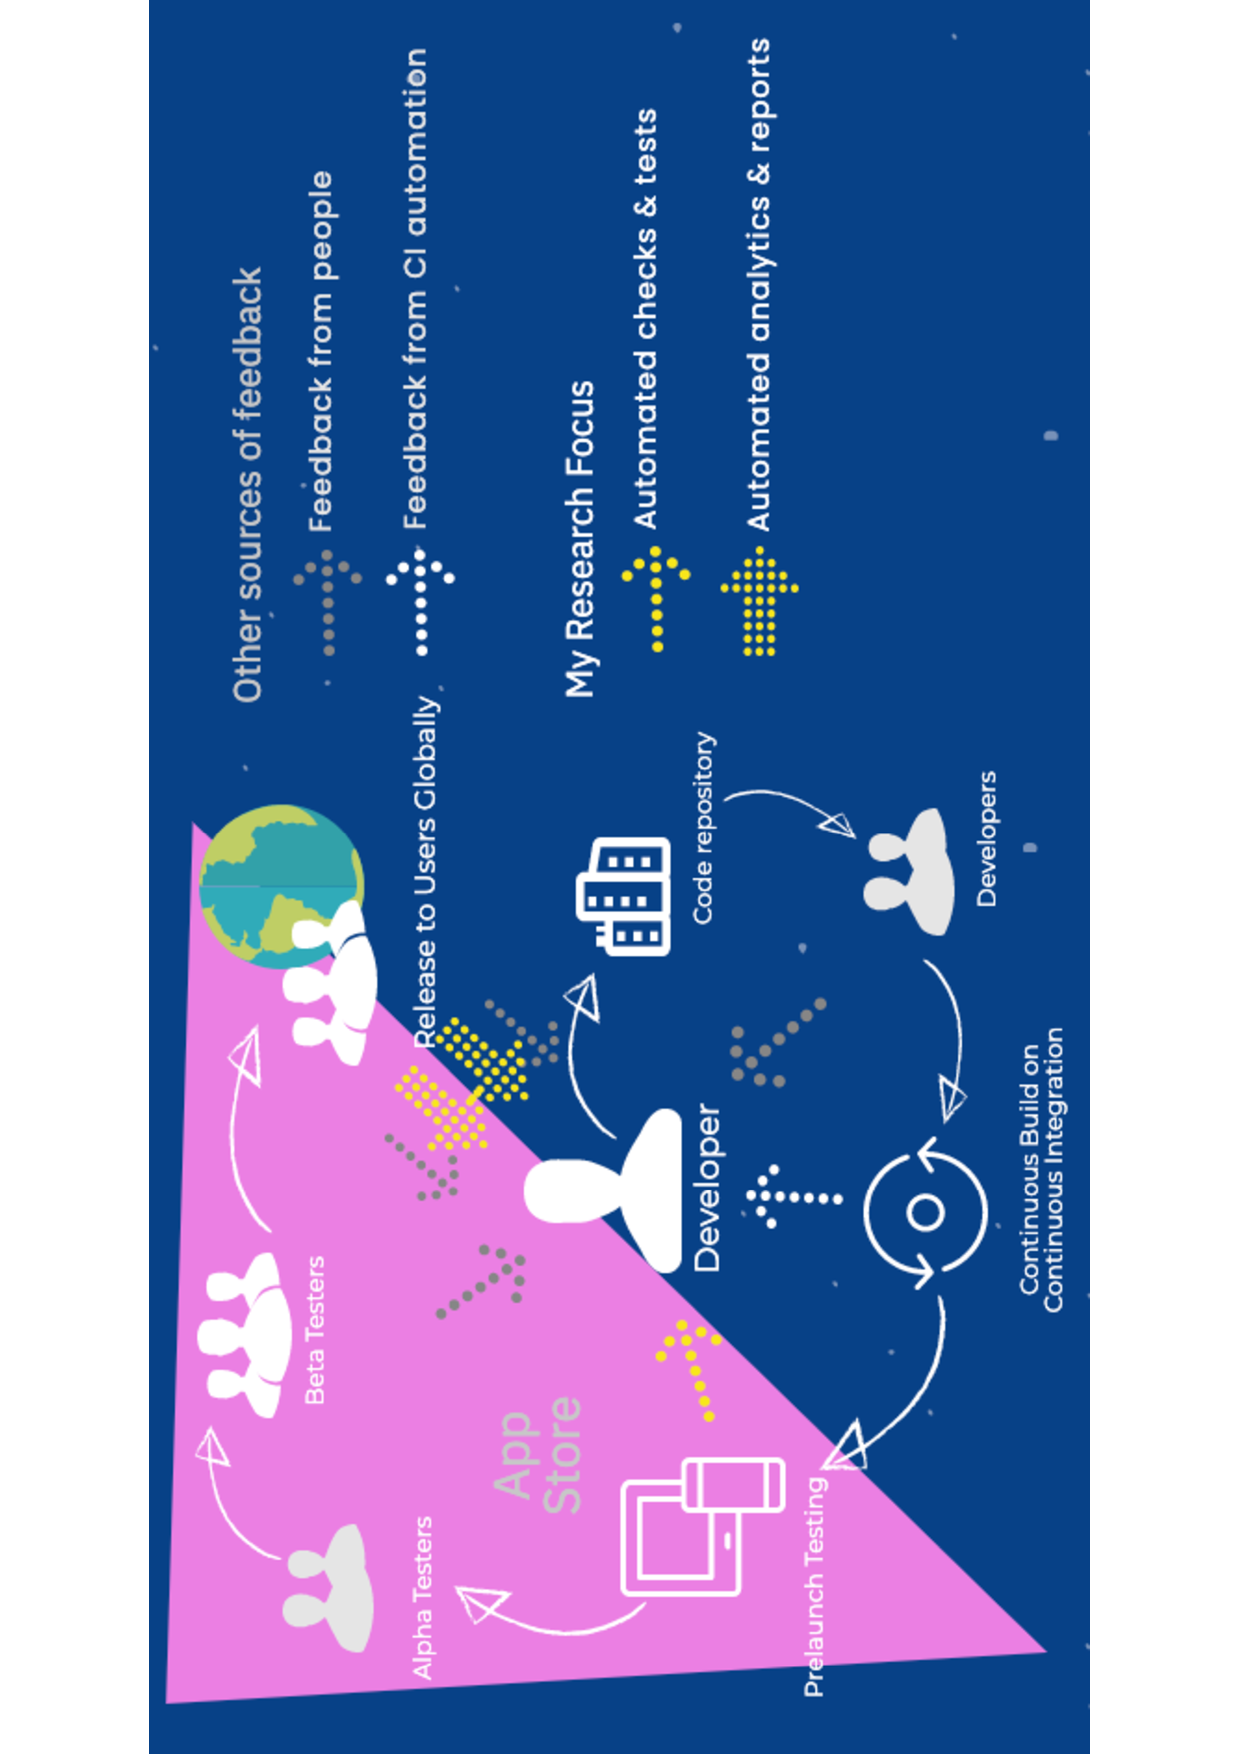
\includegraphics[width=\linewidth]{images/mobilesoft/silvias-developer-centric-figure-mobilesoft2020.pdf}
    \caption[Sources of feedback for developers]{Sources of feedback for developers \\The Research focuses on automated checks and tests performed by the app store, automated analytics and reports both in-app and at the platform level. \\ \\Other sources of feedback available to developers includes feedback from people and feedback from their development tools and CI automation.}
    \label{fig:sources-of-feedback-for-developers}
\end{figure*}

% TODO if the following footnote is split across 2 pages then review https://texfaq.org/FAQ-splitfoot to prevent an entire page becoming a hotlink for the URL in the footnote.
Developers have various sources of feedback about their apps, as Figure~\ref{fig:sources-of-feedback-for-developers} illustrates~\sidenote{Image created in pikochart \url{https://create.piktochart.com/teams/16497973/infographic/saved/47760961?}, a paid for online editing tool. Thanks to Silvia Harty for her help designing the original figure.}. The pink triangle represents the extent of Google Play (the app store) in terms of providing feedback. Other feedback is also available independently of the app store, for instance: from the development process, and by using software incorporated directly into the app that provides bi-directional communications between the development team and end users~\sidecite{avellis_harty_yu_towards_mobile_twin_peaks}.


Each source of feedback may stem from humans (for example, in reviews) or from software (for example, from code quality tools such as Lint).This research introduces three sources of software-generated feedback:
\begin{enumerate}
    %\setlength\itemsep{-0.5em} %\itemsep0em 
    \item Prelaunch testing: automated checks and testing provided by the app store (Google Play),
    \item platform-provided analytics: automated analytics and reports gathered by the Google Android platform from users devices configured to provide the underlying data,
    \item in-app error reporting (including crash reporting): software added by the app development team to detect and report crashes, and optionally errors and similar/related data.
\end{enumerate}

% NB: Alpha and Beta channels formed part of one of the major industry case studies. Clearance has not yet been granted to write or publish the findings.

Note: while the first two of these sources use Google Play as their source, other app stores and similar ecosystems may provide equivalent sources of feedback.

\section{Research Questions}
\label{section-research-questions}
%%%%%%%%%% Isabel Evans suggests adding a table with my RQs at the start of this section. TBD. COULD-DO. Certainly it seems this section needs polish.

%MUST-DO \yijun{If possible, you may need to dig out a few MobileSoft research papers to give evidence that these research questions have not been addressed in literature, e.g., \emph{Future Trends in Software Engineering Research for Mobile Apps}~\sidecite{nagappan2016_future_trends_in_sw_eng_for_mobile_apps}, whether the future work of some paper suggests one does not know the sources, value, or impact of mobile analytics to assess and improve app quality? Is there nothing in the general SE literature studying the "analytics" to "general software quality" problem? If there are such general work, how does "mobile analytics" and "app quality" differentiate the RQs to existing ones...}


My research hypothesis is that using mobile analytics can help improve the work development of teams and the quality of the products they create. Here work includes the development, testing, and bug investigation of the software being created. For the quality of the product, this research is focusing on a subset of qualities which are \gls{glossary-technology-facing}, %technology-centric, 
and in particular the \gls{glossary-reliability} and \gls{glossary-stability} of the mobile apps when they are in use. This research builds on prior work on software analytics for mobile apps and focuses on its practical application by software development teams to improve app reliability. This is important because app reliability, as measured by crash rates and ANRs, is key metric in the mobile app ecosystem. Because this metric is used by the platform provider to determine whether an app should be given access to the ecosystem, it is something developers should pay attention to. In order to understand the effect of applying mobile analytics on the software development practices for improving reliability of apps, we need to explore the processes, artefacts and tools associated with these activities. This research investigates these three dimensions based on case studies of different mobile app projects, to identify both the current practices and opportunities for improvement provided by using mobile analytics.

The core question investigated by this research:

\begin{quote}
  \emph{How can applying mobile analytics in software development practice improve the reliability of mobile apps?}~\label{overall-research-question}\index{Research questions}
\end{quote}
% Thanks to https://tex.stackexchange.com/questions/35933/indenting-a-whole-paragraph

To expand on the research question:
\begin{itemize}
    \item \textbf{Applying mobile analytics}: is the use of mobile analytics in order to effect improvements to the practices and the artefacts. Applying mobile analytics refers to both collecting data from the usage of the app and also making use of the analysis of this data to identify and address issues that can improve the app. Improvement of the app focuses on increasing the stability/reliability by reducing ANRs, crashes, and through improving how the app handles various errors (typically reported through Exceptions~\footnote{Exceptions are a core construct in Java programs intended to make those programs robust~\cite{robillard2000_designing_robust_java_programs_with_exceptions}, and similarly \glspl{glossary-exception} are core to Android apps}).
    \item \textbf{Mobile analytics}: Analytics where the data is collected by software running on mobile smartphone-based devices pertaining to the app's qualities-in-use. This research focused on analytics collected pertaining to the stability of the app, where stability includes the reliability of the app.
    \item Software development: includes tasks performed by the software developers including design, coding, testing, bug reporting, and bug tracking.  Use of Scrum development practices, following recommendations and guides that include application compatibility, \gls{ui} guidelines, and designing for performance and responsiveness, \emph{etc}. [Software] testing~\sidecite[][pp.398 - 399]{wasserman2010_software_engineering_issues_for_mobile_app_devt}.~\sidenote{This short paper skims over topics without evidence developers actually do them. Their survey, cited in this paper isn't available so appears to have not actually been published.}
    \item Reliability and Stability are two intertwined measures of software quality in use. There are contradictory opinions on their relationships to each other and to their contributions to software quality, these will be discussed in Chapter~\secref{chapter-related-work}. 
    \item In practice: the key scope of measurement focuses on the efficacy in real-world projects from the perspective of software practitioners who develop mobile applications.
\end{itemize}

In order to answer this research question it is appropriate to consider improvements to the \emph{app i.e. the product} and to the \emph{processes/practices} development teams apply when they develop and maintain their mobile apps. Improvements cannot be be usefully considered in isolation, they need to be grounded in the current practices: the developers will have their perspectives on their use of mobile analytics, and their development artefacts may provide cross-verification of what they say they do compared with tangible evidence of how they use those mobile analytics tools. 

Furthermore, there may be constraints and/or limitations in the current mobile analytics tools which may adversely affect the improvements development teams are able to make to their processes/practices and to their products, hence it is also germane to consider improvements to the current mobile analytics tools.

These additional supporting questions can be restated as six distinct yet related perspectives.

\begin{figure*}
    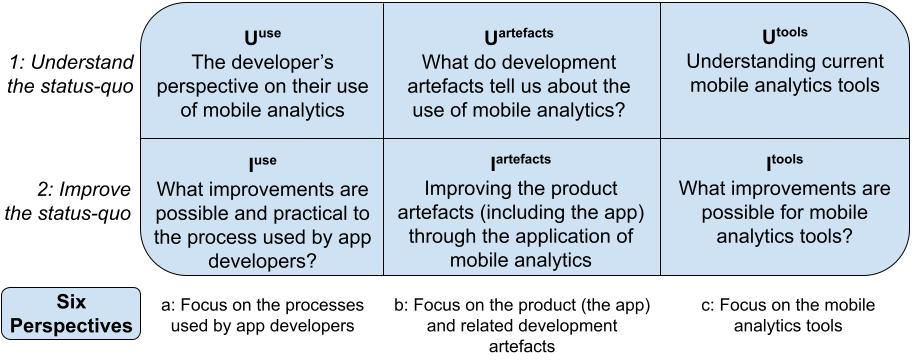
\includegraphics[width=\linewidth]{images/my/six-perspectives-2x3-matrix-12-nov-2021.jpeg}
    \caption{Six Perspectives of Mobile Analytics}
    \label{fig:six-perspectives-in-the-research-questions-section}
\end{figure*}

\subsection{Research questions lead to six perspectives}~\label{rq-leads-to-six-perspectives}
The six perspectives are illustrated in Figure~\ref{fig:six-perspectives-in-the-research-questions-section}~\sidenote{Source figure:~\href{https://docs.google.com/drawings/d/1SafKu3uqgl-s8-I8iWSSWmFY4NdlNpw8v6ZiJDGh50c/edit?usp=sharing}{Google Docs: Six Perspectives drawing}.} and paraphrased below:

\begin{enumerate}
    %\setlength\itemsep{-0.5em} %\itemsep0em
    \item [1a] What do app developers say they do in terms of using mobile analytics? (understand the \emph{status quo} from their perspective).\index{Research questions}
    \item [2a] What's possible in terms of improving their processes, their practices through using mobile analytics?)
    \item [1b] What does their source code (and other available development artefacts) tell us about their use of mobile analytics? (\emph{i.e.} to understand current behaviours in terms of the code that's implemented.
    \item [2b] What's possible in terms of improving the product (and particularly the mobile app) through the application/use of mobile analytics?
    \item [1c] What do we learn about various current mobile analytics tools?
    \item [2c] What improvements are possible for mobile analytics tools based on what was learned in the various case studies?
\end{enumerate}

These provide clear grouping for each of the three columns: on processes (a), on apps and related development artefacts (b), and on the analytics tools (c) which are considered in terms of first understanding and then improving the \emph{status-quo}, shown as two rows, \emph{i.e.} a 3x2 matrix. 


% https://www.skmurphy.com/blog/2014/01/27/difference-between-a-hypothesis-and-an-assumption/
Here the hypothesis is that analytics can help, as stated by Buse and Zimmermann ~(\citeyear{buse_analytics_2010}); and \emph{``with explicit and implicit feedback now available (almost) continuously, questions arise. How can practitioners use this information and integrate it into their development processes [to decide when to release updates]?"}~\sidecite{maalej2016_towards_data_driven_requirements_engineering}.


\section{Research contributions}
Before this research little was known about developers integrating mobile analytics into their artefacts and/or their processes. Unknown were - how, why, and when, they used the outputs of the mobile analytics. Similarly, the effects of using mobile analytics in terms of any changes to the reliability of these apps was not known. Furthermore, little was known about the mobile analytics tools and services used by app developers in industry or in real-world mobile apps.

\subsection{My contributions to knowledge}
The research contributes to the understanding of tools and information seldom available to research - of professional app developers, their artefacts, and of professional mobile analytics tools and services. 

\newthought{Processes}: 
My research contributes knowledge on the approaches various app development teams apply when they use mobile analytics including the selection, integration of code and services, and their application of mobile analytics to detect, identify, and address errors and failures reported by mobile analytics. It builds on prior research, for example, on Insight, and confirms their findings. It contributes new knowledge in the adoption platform-level and commercial in-app mobile analytics, including a) usage patterns by development teams ranging from individual  developers, small teams and large,  \gls{glossary-sharded}\sidenote{\href{https://en.wikipedia.org/wiki/Shard\_(database\_architecture)}{Wikipedia: Shard (database architecture)}} teams, and b) public opensource projects, hybrid projects that combined private and proprietary practices, through to a development team at a major corporation.

Some of the findings were surprising in terms of the patterns of use and in the efficacy of using mobile analytics to achieve significant improvements.

Development teams who embedded mobile analytics into their ongoing, core practices, were able to achieve highly reliable and stable apps. 

\newthought{Artefacts}: 
The research extended prior art in studies of opensource mobile app codebases, with a focus on the use of the most popular product offering: Firebase Analytics. Developers often incorporated multiple mobile analytics libraries into a single mobile app, each for a specific purpose. When developers addressed failures reported by mobile analytics they often modified the source code of the app; these modifications were generally small, yet the effects on improving the reliability/stability of the app were material. 

It also contributes insights from proprietary, commercial codebases and issue tracking artefacts where development teams intermittently filed bug reports for issues reported by mobile analytics.

\newthought{Mobile  Analytics Tools}:
The research identified characteristics of a wide range of mobile analytics tools that serve Android app developers in particular. It also found and  presents a range of flaws found in professionally-developed mobile analytics tools, including several of the most-used mobile analytics offerings.

The research contributes material relevant to professional app developers and to the developers of mobile analytics. 

Improvements were identified in all three areas and some of these were implemented during the research. 

Note: In addition to specifying my research contributions add explicit summaries of my contributions that have already been published.

\subsection{Practical impact of my work}
Several of the tool development organisations including Amplitude, Google, and Iteratively actively sought insights and updates from my research. They improved various aspects of their respective mobile analytics offering.

App developers who applied the techniques described in my research were consistently able to significantly improve the reliability/stability of their apps.


\section{Outline of this thesis}
At a high-level thesis is in three main parts: the preamble which includes chapters 1 to 5, the findings in chapters 6 to 8, followed by the discussion, conclusion, and future work in chapters 9 and 10. There are two short appendices: on thematic analysis, and additional details for some of the mini-experiments.

\bigskip

This thesis starts with an introduction to the context of investigation - mobile app development - together with an exploration of the state of the art. Based on this, the method adopted for conducting the research is presented before outlining the different mobile app and analytics tool case studies. Following this, the findings are set out, covering three thematic areas relevant to the use of mobile analytics: app development processes and the use of analytics, apps and their artefacts, and mobile analytics tools. Finally there is discussion of the findings together with potential areas for future work. A more detailed outline of the remaining chapters of the thesis is set out below.

\newthought{Chapter 2 | Preparing the ground:} this chapter prepares the ground for the rest of this thesis by explaining contemporary development practices for mobile apps. It then presents five conceptual models related to mobile apps. These are followed by several, relevant, practical details.

\newthought{Chapter 3 | Related work:} explores the state of the art relevant to software quality, software analytics, and the mobile app ecosystem.

\newthought{Chapter 4 | Methodology:} sets out the research approach adopted to gather and analyse data for the different case studies explored as part of the research.

\newthought{Chapter 5 | Overview of the case studies:} introduces each of the app-centric and tool-centric case studies using a consistent structure to make them easy to comprehend and to facilitate comparison.

\newthought{Chapter 6 | Findings - Analytics in use:} presents the key findings from the case studies relevant to the use of analytics by mobile app development teams.

\newthought{Chapter 7 | Findings - Apps and their artefacts:} discusses the findings relating to the software developed in the different mobile app case studies, together with their associated artefacts.

\newthought{Chapter 8 | Findings - Mobile analytics tools and their artefacts:} Focuses on the mobile analytics tools explored during the course of the research and the different artefacts produced by these tools.

\newthought{Chapter 9 | Discussion:} Explores the findings across the different perspectives of the research in relation to the wider literature of software quality and mobile app development practices.

\newthought{Chapter 10 | Conclusions and future work:} Summarises the key contributions of the research and discusses avenues for further investigation.


\chapter{Preparing the ground}
\label{chapter-preparing-the-ground}
\emph{`...there is nothing new under the sun. \\Is there anything of which one can say,``Look! This is something new"?'}~\sidenote{\href{https://www.biblegateway.com/passage/?search=Ecclesiastes+1\%3A9-10&version=NIV}{Ecclesiastes Ch:1 vv. 9-10 NIV edition.}}

\setkeys{Gin}{draft}
\julian{This chapter is currently in draft compilation mode to try and stop timeouts on Overleaf. See \url{https://www.overleaf.com/learn/how-to/Optimising_very_large_image_files} for details.}
\vspace{10mm}

This chapter provides a grounding in the domain of mobile apps, how developers obtain information, and mobile analytics,~\emph{etc.}  
% MUST-DO revise opening sentence and remove the etc. via \akb
For any individual elements there may be much that is known and seemingly little novelty. And yet, it has become clear that when these elements are combined an interesting and rich domain emerges that can serve developers of their mobile apps.

While this discussion of the mobile app ecosystem aims to be as detailed and accurate as possible, there are limits to which this is possible in the context of closed, proprietary systems including those discussed in this thesis. 

To improve readability the thesis includes some generalisations rather than using qualifiers throughout, such as often, mainly, and so on, unless they materially reflect variations in people's experiences.

The chapter introduces five 
%MUST-DO revise this and the next paragraph once the chapter's contents have settled down.
conceptual models, including: a model of apps and app stores, layers of an app and observation points, of analogue and digital feedback, usage analytics, and finally DevOps. These concepts help us understand key considerations for mobile app developers and what they are working with.

The chapter continues with five practical aspects including app development and usage, information sources for developers, and choices for engaging with analytics. Developers need to address these as part of being effective in their work and providing apps of adequate quality. Mobile analytics can provide useful sources of information, including problems with the apps in use, and mobile analytics can complement and calibrate other sources of quality related information including software testing. 


\section{Potential sources of evidence}~\label{sec:potential-sources-of-evidence}
\emph{Note: this was moved from the Introduction and may have a better home. \textbf{MUST-DO} integrate this section in this chapter.}
%\emph{What can we learn from people? what can we learn from analytics? ...?}

%\textbf{How can we know about mobile analytics and the effects of using them?}

%\nth{16} Jul 2021:~\akb{This subsection is too verbose. Summarise with a diagram showing sources of knowledge and links to difference types} - \textbf{MUST-DO} and will do once I make sense of where's the best place to put this material. For now I've moved the overall \href{section-ontology-and-episetemology}{\nameref{section-ontology-and-episetemology}} section to after the RQs and before the methodology section.

%Here we consider the questions: (1a) What we can know about mobile analytics and (1b) how we can know it? Then more specifically, these related questions are key given this research focuses on using mobile analytics to help answer the next question. (2) How we know about the identification and measurement of some flaws in behaviour of software that are considered measures of quality of the software in use?

Broadly we can learn from people, use \textit{software analysis tools}~\sidenote{MUST-DO add a paragraph on software analysis tools.}, and use data to answer these questions. In some cases the data comes from a single source, in others cases from several.

\textbf{Software analysis tools} 

Lint~\sidenote{\href{https://developer.android.com/studio/write/lint}{Android Lint} or \href{https://github.com/realm/SwiftLint}{SwiftLint} for iOS.}


\textbf{Mobile analytics} comprises software, systems, and sometimes services. Broadly we can read about them, study their source code, analyse, test, and use them directly, and ask others for their perspectives and insights. Rather than go into lots of detail here, several of the appendices of this thesis cover aspects of mobile analytics, in particular, in~\href{app:on-mobile-analytics}{\emph{\nameref{app:on-mobile-analytics}}}.

In terms of learning from \textbf{people}, we can do so by asking the designers, constructors, operators, and users of a system. However, we're also limited by who we can ask, what they are willing/able to communicate, and whether that communication is sufficiently open and transparent to be useful and reliable. We can also learn from information produced by people, and in particular for mobile apps we can use ratings and reviews. Given human behaviour it may also be worth considering aspects such as the provenance of the information sources, fake data, \emph{etc.} especially where there are rewards for slewing the results of the measurements being used in an ecosystem.

We can know through \textbf{static analysis} tools, automated tests, end-to-end testing, \emph{etc.} and all of these are used by at least some of the developers of mobile apps some of the time. They often take place \textit{before} the software is released to end users.

We can also know through data collected when the software is used. As~\sidecite{RFC3164} notes in RFC3164, ~\emph{``Since the beginning... operating systems, processes and applications were written to send messages of their own status, or messages to indicate that certain events had occurred. These event messages generally had local significance to the machine operators."}. Mobile apps also write messages locally and developers use them for similar purposes (nuances and differences are discussed in the related work chapter). These local messages can be read by humans locally and/or read by software that delivers them elsewhere. Developers can also add software to their apps to log information for processing elsewhere which is where much of mobile analytics and crash reporting fits in the scheme of things.

Log messages are written locally on the same device (\textit{i.e.} computer) that runs the software. When developers are developing the software they tend to be local to the device and therefore able to read the logs. When the devices are remote, as they are for end users of mobile apps, developers cannot easily access the logs or read them. If they wish to do so they need mechanisms to obtain the logs. They can choose to incorporate mechanisms into the app including custom logging mechanisms that transmit the logs so they can be processed remotely. They can rely on log forwarding software~\sidenote{For instance a fairly involved example for Flutter Android apps, using MQTT, is described in~\cite{adil2020_sending_logs_from_flutter_apps}}, and/or mechanisms provided on the device if they exist.
% A couple of Android implementations for LogStash include:
%  https://github.com/Labgoo/android-logstash-logger
%  https://gist.github.com/PatrykGala/55603fe4259d812fdc0ffbc9e63eaabc (saved in my references)


Various data can be potentially collected implicitly and explicitly. What can be collected depends on the observation mechanisms. Observation may be within an app or external to it, for instance by the operating system as both iOS  and Google Android do~\sidenote{There are other custom versions of Android, for instance used in Amazon Kindle Fire devices. Their details are outside the overall scope of this research.}(details in the Appendix titled~\href{chapter-on-mobile-analytics}{\emph{\nameref{app:on-mobile-analytics}}}). Within an app the observation may focus at a single layer, for instance the visual user interface, or several. The choices of observation mechanisms within an app are made by developers or their stakeholders. The choices external to an app can be made by various people including the platform provider, users, or indirectly using other software including third-party apps, spyware, accessibility software, and so on.

Analytics, such as user-journeys, can help to answer questions about the usage of the software. They help establish \emph{what-is}. As we understand more about what-is we can then consider \emph{what-would-be-better} and do gap analysis between what-is and what-would-be-better.

%See https://tex.stackexchange.com/questions/348298/svg-package-includesvg-with-underscores-in-svg
\makeatletter
\DeclareRobustCommand*{\escapeus}[1]{%
    \begingroup\@activeus\scantokens{#1\endinput}\endgroup}
\begingroup\lccode`\~=`\_\relax
    \lowercase{\endgroup\def\@activeus{\catcode`\_=\active \let~\_}}
\makeatother

%See https://tex.stackexchange.com/questions/390804/how-to-scale-text-in-svg
% PS: I could try https://tex.stackexchange.com/questions/113282/text-size-in-inkscape if I run into problems with the current approach.
\begin{figure*}
    \copyrightbox[r]{
        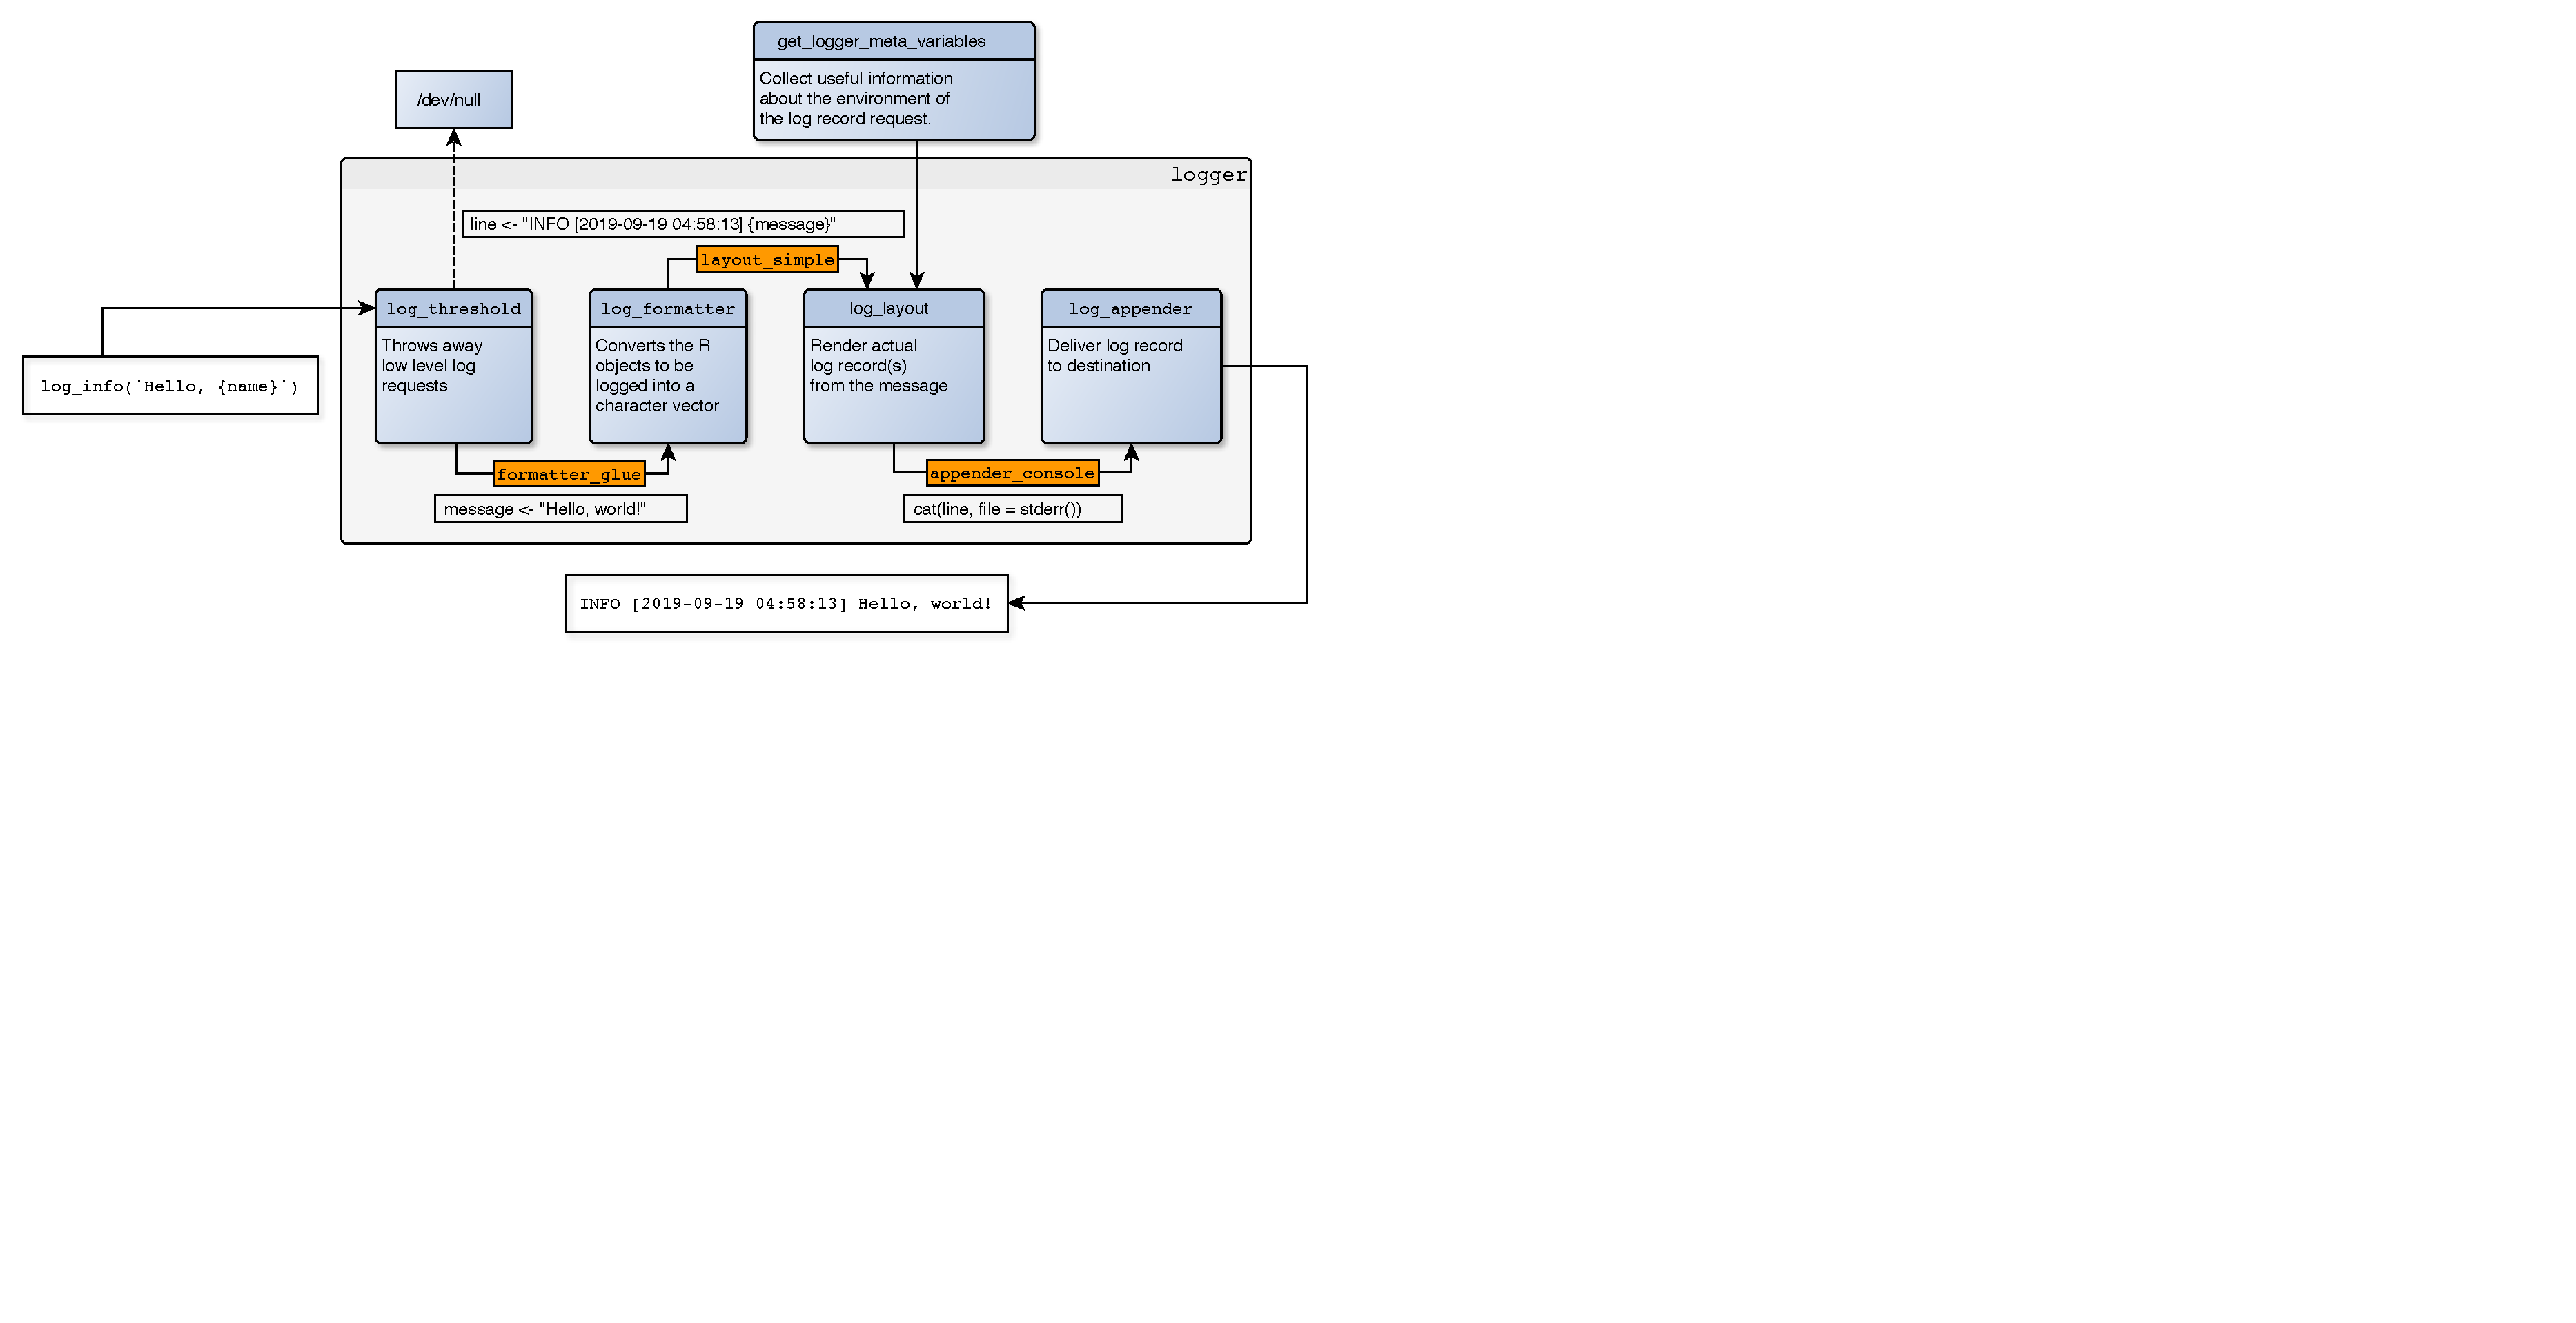
\includegraphics[width=\linewidth]{images/github/loggerstructure.pdf}}
    {\textcopyright \href{{https://twitter.com/daroczig}}{daroczig}\\source: \href{https://github.com/daroczig/logger/blob/master/vignettes/logger_structure.svg}{logger\_structure.svg}}
    \caption{TEMP - to be replaced: Logger Structure from an R Logger project - TBC whether to provide something similar}
    \label{fig:temp_logger_structure}
\end{figure*}

\begin{comment}
%This is a simpler structure without the copyright box. Commented out for now, kept in case I want to switch quickly.
\begin{figure*}
    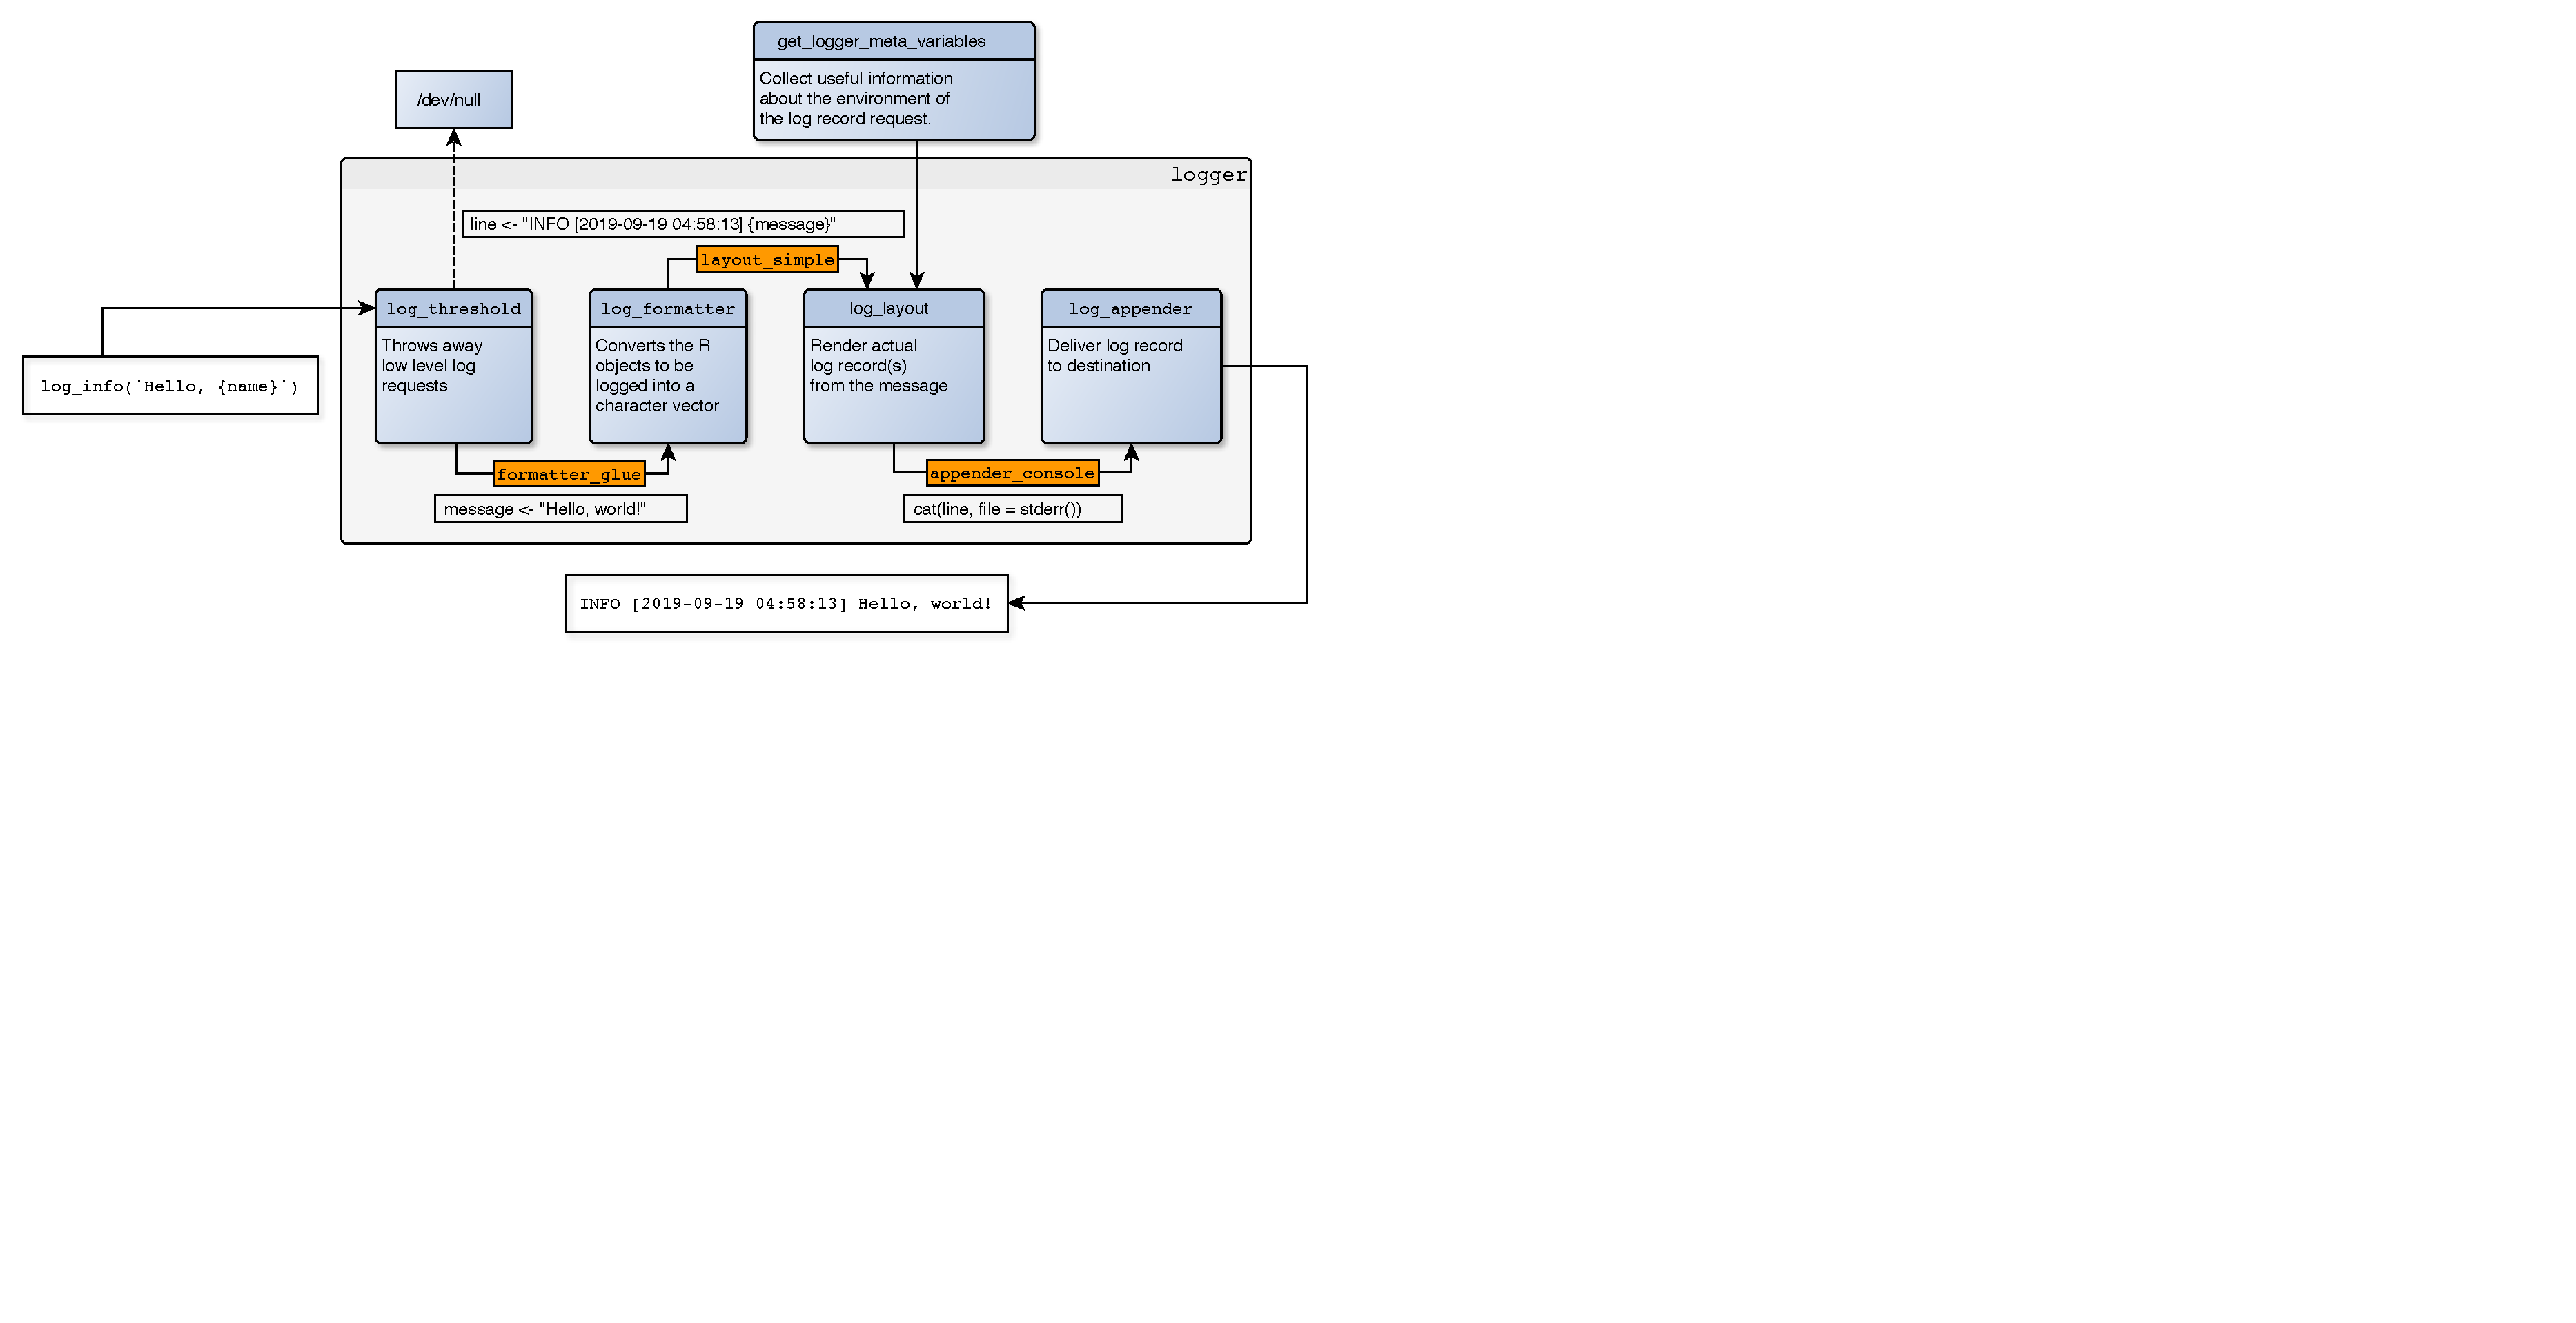
\includegraphics[width=\linewidth]{images/github/loggerstructure.pdf}
    \caption{Yin Yang to represent DevOps}
    \label{fig:yinyang_for_devopsxxx}
\end{figure*}
\end{comment}


\textbf{Reporting/generating and Observing}: What happens within the app stays within the app unless someone looks inside the app or the app reports what's occurring. Observation without action limits the utility of whatever is learned.  \textbf{SHOULD-DO}, it'd be great to have a figure similar to \url{https://github.com/daroczig/logger/blob/master/vignettes/logger_structure.svg} for platform-level analytics. Temporarily it's included here in Figure~\ref{fig:temp_logger_structure}.


Survivorship bias (\sidecite{wikipedia_survivorship_bias}) is relevant to understanding the information developers receive, some data does not `survive' the journey from source to developer. And much of the information that is does reach the developers does not survive or, perhaps better put, thrive in terms of being used productively. They have plenty of other demands for their time and attention and much of what could be useful isn't used in practice, therefore the data needs to be sufficiently useful and relevant and improvements tractable for any proposed approach to be used long term in practice.


Discuss which sources are likely to provide input to the key elements needed to underpin the RQs.

\textbf{MUST-DO} Segue to the research strategy and how we devise a feasible approach that uses as many of these sources as practical.



\section{Development practices for mobile apps}
Few if any developers write perfect software, and this applies also to developers of mobile apps. 

%SHOULD-DO Add the Amphitheatre illustration. And suitable words to explain the concepts.

This section introduces the concept of \textit{Zones} as they apply to finding and potentially fixing issues while developing software. The concepts are inspired by various sources including agile development practices, release management for mobile apps, computer networks, and particularly the use of firewars and `de-militarised-zones' (known as DMZ). 

\subsection{Control (find-fix) zones}
A find-fix Zone incorporates the scope of finding issues and being able to fix, or at least ameliorate, them. Where issues are discovered in the local Zone, developers can fix the issue without needing to involve others (however they can choose to do so), and indeed some may consider these issues an intrinsic and essential part of iterative software development. Other zones extend beyond the immediate developer and involve other people.

For the purposes of my research I have identified three categories of zones:
\begin{enumerate}
    \item \textbf{Local Zone}: This is local to the developer of software, tests, resources, designs, and so on.
    \item \textbf{Mezzo Zone(s)}: These zones involve other people, they may be peers, team members, other people in the organisation, trusted testers, and so on. There may be anything from virtually no zone for solo independent developers working on their own app, to a plethora of zones involving various stages of pre-release testing, checking and approvals in large corporate organisations.
    \item \textbf{Live Zone}: End users are able to use the released app. The app is finally able to potentially achieve business objectives. 
\end{enumerate}

\begin{figure*}
    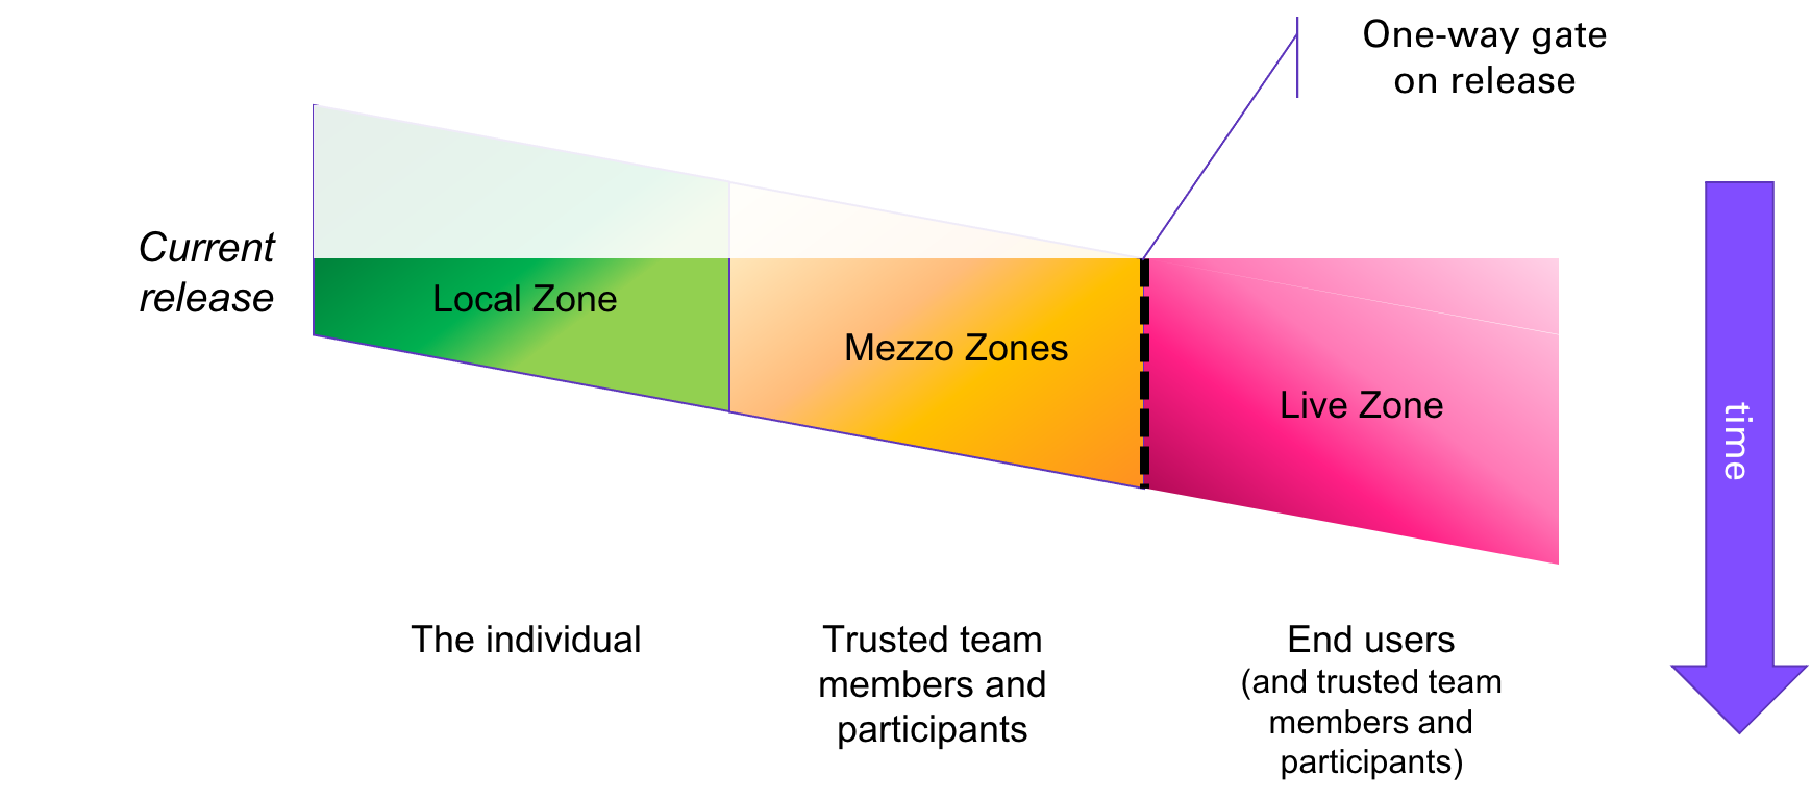
\includegraphics[width=\linewidth]{images/my/control-find-fix-zones-a.pdf}
    \caption{Control find-fix zones}
    \label{fig:my:control-find-fix-zones-overview}
\end{figure*}

These three categories of zones are illustrated in Figure~\ref{fig:my:control-find-fix-zones-overview}. The figure includes a one-way gate, that behaves like the Rubicon in Julius Caesar's time~\sidecite{wikipedia_rubicon} where the die is cast once a release has been launched in the app store. The release cannot be reverted, at best it can be paused or superseded with another subsequent release. The app now comes into contact with end-users and is expected to achieve the business objectives of the organisation who made it available.

\begin{figure*}
    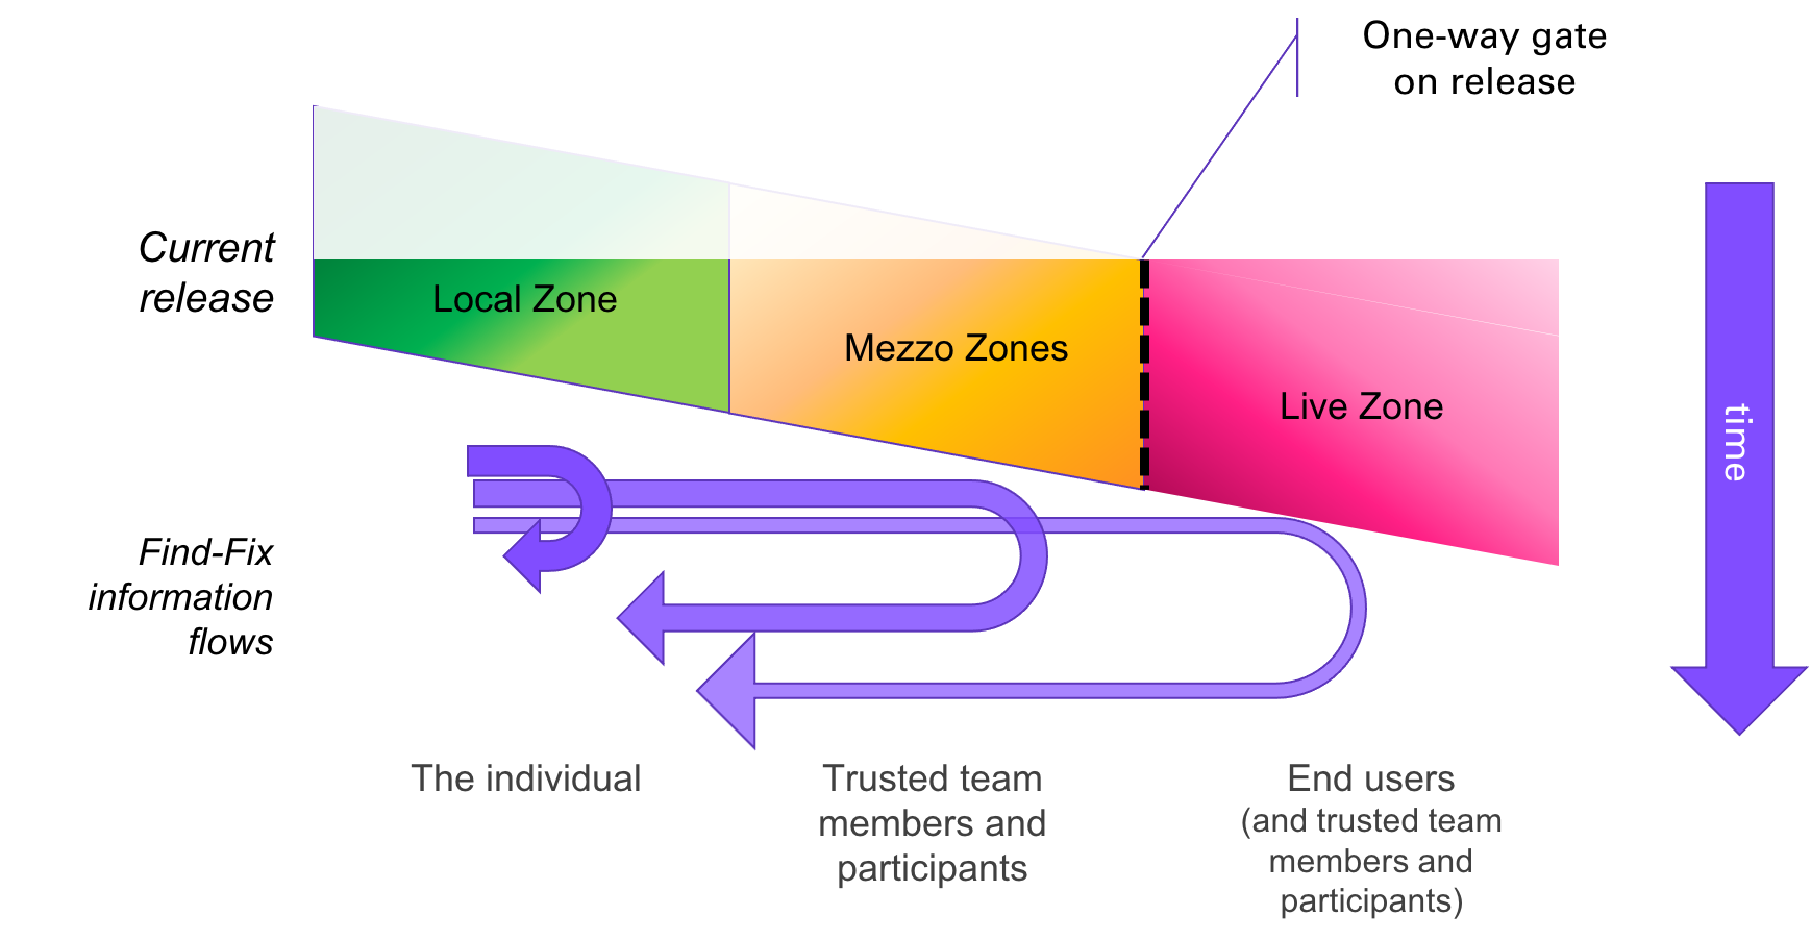
\includegraphics[width=\linewidth]{images/my/control-find-fix-zones-with-information-flows.pdf}
    \caption{Control find-fix zones with information flows}
    \label{fig:my:control-find-fix-zones-with-information-flows}
\end{figure*}

Figure~\ref{fig:my:control-find-fix-zones-with-information-flows} is a modified version of Figure~\ref{fig:my:control-find-fix-zones-overview} that includes the find-fix information flows. Assuming fixes are made be the development team for the app (rather than improvements that can be addressed in servers, through configuration changes, and so on) then the information about flaws and issues needs to reach that development team somehow. For issues found in external releases (\emph{i.e.} those made available to end-users) 

When issues are discovered before the software is released there is the possibility of the developer being able to address them before the software is released (they stakeholders may choose to delay the release to allow this to happen). Where issues are discovered in the released app, unless there are viable mechanisms to patch the app, the fix needs to be made in a subsequent release \textit{and} the end-user needs to use the subsequent release to receive the benefit of the release.

There are two key challenges:
\begin{enumerate}
    \item the developer learning about issues in sufficient detail to potentially address them,
    \item being able to address issues and provide the benefit to users who are, or  may be, affected by it.
\end{enumerate}

Both these aspects are covered next in terms of the bug-fix process for mobile apps.

\subsection{Bug-fix process for mobile apps}
%MUST-DO move the following comment to the next chapter once I've drafted the relevant illustrations.
% In my view, mobile analytics helps in the 'current' timeframe of the development and release process, in that it can provide ranked notifications of various issues (including 'stability' failures: i.e. crashes and ANRs) on a timely basis. 

Given apps have been released and users are using those releases then - there may be issues in the app exposed while it is in-use. Some of these may be noticeable (or perceivable) by the end-users, others not. These issues include 'stability' failures: \textit{i.e.} crashes and ANRs and performance-related issues \textit{e.g.} slow responses, excessive power and network consumption, and so on.

Sources of failures when an app fails a user include: code written by the developer or their colleagues (where they have control over the source code and can modify it as they see fit), third-party libraries (which are used extensively in mobile apps and where developers can replace, up- or down- grade the library but little else), or the platform, including platform-provided code.

For the development team to actively address any of these failures they need to be aware of them and have sufficient details to take action. Figure~\ref{fig:my:bug-fix-process-for-mobile-apps-in-prod} illustrates past, current, and future, activities for current and future releases of an app. We will return to this figure %in this section and 
in the next chapter where the effects of applying analytics to the development process is considered.
%MUST-DO make sure I do return to {fig:my:bug-fix-process-for-mobile-apps-in-prod} in the next chapter, on applying analytics.

\begin{figure*} %[!htbp]
    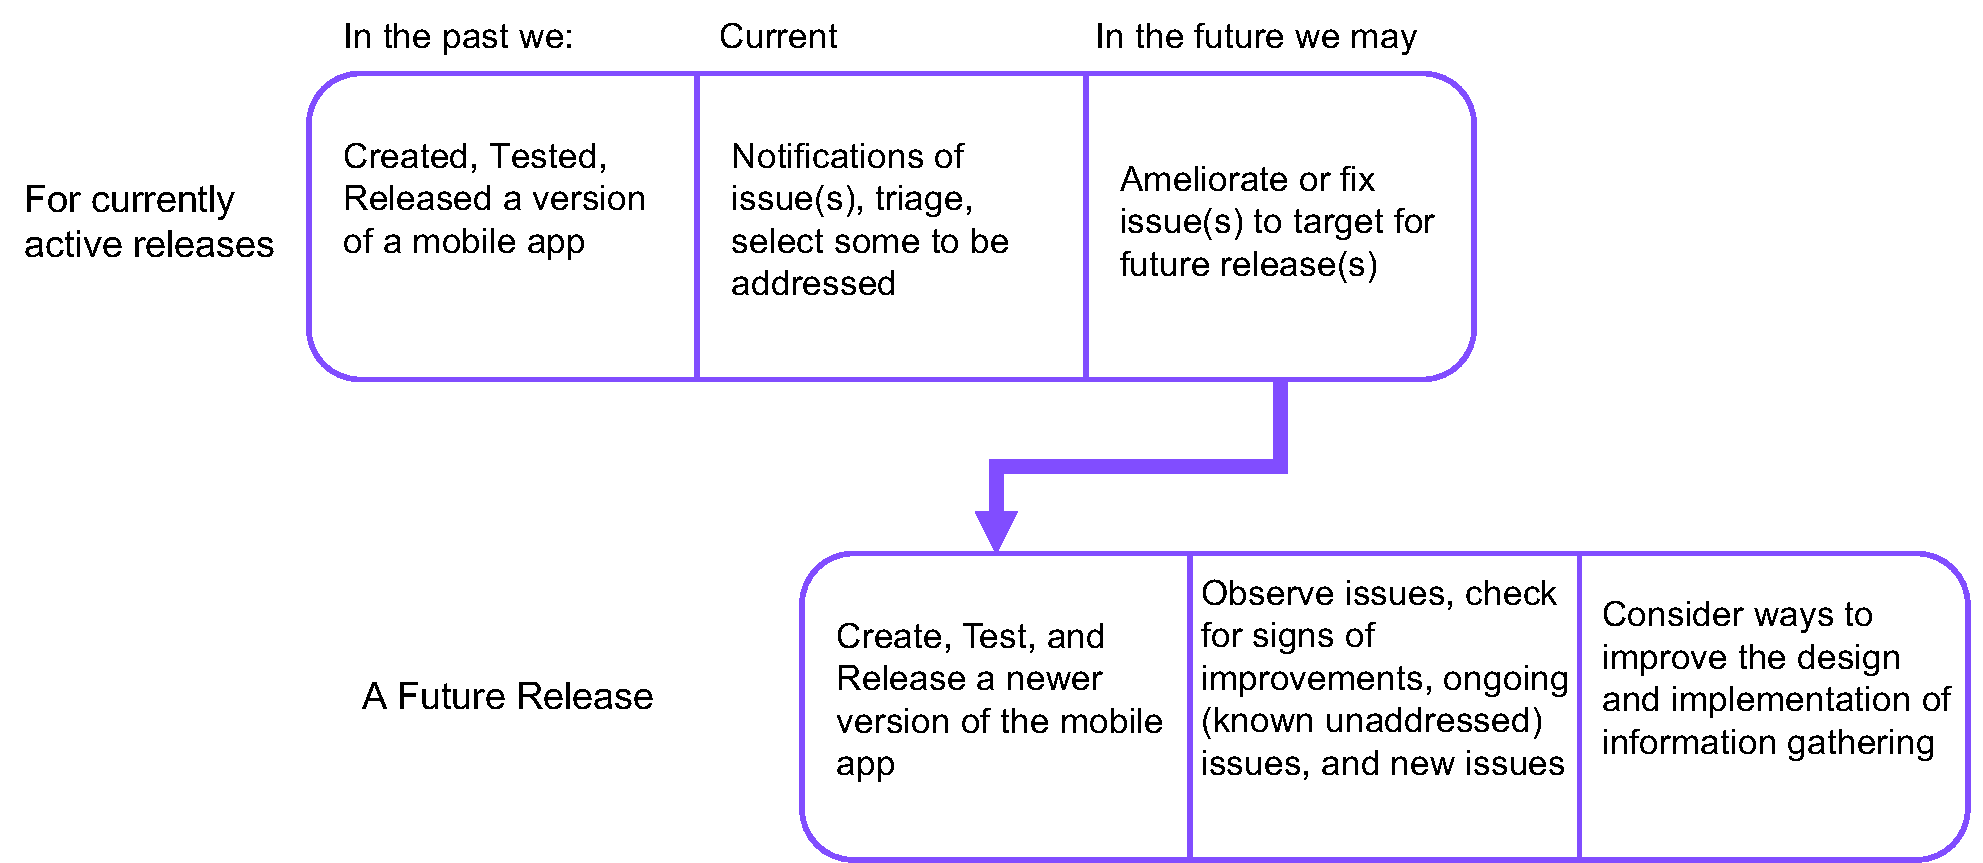
\includegraphics[width=\linewidth]{images/my/production-bug-fix-process-for-mobile-apps.pdf}
    \caption{Bug-fix, process for mobile apps in production}
    \label{fig:my:bug-fix-process-for-mobile-apps-in-prod}
\end{figure*}


Developers might learn of some of these issues from other sources e.g. from colleagues who use the app, from end-users who report issues (e.g. in reviews in the app store, on social-media, and even using in-app feedback if the app's functioning sufficiently etc.). 
% MUST-DO refer to research in automatically creating automated tests to reproduce crashes and discuss some of the limitations of that research vector. Note: this might be covered in the related works chapter.
However in my experience, and based on other research, only a subset of the issues are reported by a small subset of people who use the app~\sidenote{Estimated as 1\% by the company Raygun~\url{https://raygun.com/about}.} % Only 1% of customers actively report errors and performance issues they encounter whilst using web and mobile applications.
, and certainly not all users report all the stability issues all of the time. Google added a feature to Android 2.2 to enable users to easily send crash reports to Google which Google presented on the `Bugs' tab to the app developer~\sidecite{androiddevelopersblog2012_android_application_error_reports}.

Any amelioration or fix that occurs in the app's codebase is only useful to those users who use the newer release of the app that include the improvements. Our research confirms some users continue using older releases of the app unless blocked/prohibited from doing so (there are mechanisms for doing so). Blocking/prohibiting use of older failing versions of the app may be a mixed blessing. Some users may be lost and/or upset by being forced to upgrade the app. However the stability stats in the app store may improve (assuming the intended improvements were effective).


\section{Conceptual model of apps and app stores}
This section introduces a conceptual model of apps and app stores and presents four views of apps in an app store together with various implications of the views, relationships and interactions. 

The vast majority of mobile apps are provided through app stores, and the two largest app stores:~\href{https://play.google.com/store/apps}{Google Play} and Apple's~\href{https://www.apple.com/app-store/}{App Store} both collect mobile analytics from end user's devices with permission. So, understanding the conceptual model of apps and app stores provides some context for these sources of mobile analytics. 

The concept of an App Store has existed since at least 2003, according to the co-founder and CEO of Salesforce~\sidecite{benioff_trailblazer_2019}, where the idea was proposed by Steve Jobs and later implemented as \href{https://appexchange.salesforce.com/}{\emph{AppExchange}} in the Salesforce platform. Around the same period various app stores emerged for mobile apps~\sidenote{Tens of app distribution platforms are listed on Wikipedia:~\href{https://en.wikipedia.org/wiki/List_of_mobile_app_distribution_platforms}{List\_of\_mobile\_app\_distribution\_platforms}}; and the concept seems to have been introduced around 1999 by Handandgo~\sidenote{\url{https://en.wikipedia.org/wiki/Handango}}. Academic research into the effects of app stores emerged in or around 2010, for instance with the work of Kimbler who investigated the effects on mobile operators from a business strategy perspective~\sidecite{kimbler_app_store_strategies_2010} (mobile operators lost out in the overall battle of app stores, now platform specific app stores dominate the market). 

The research is situated in apps that are available in app stores and in the Google Play app store specifically. App stores house millions of apps and serve billions of users. They also present a rich tapestry of perspectives on software apps and the ecosystem. There has been a great deal of research that focus on particular areas of these apps and sometimes connect these areas as part of the research. This research focuses on an area seldom investigated, namely it concentrates on the developer's view of how their app is perceived by the app store and whether they can improve the perception by addressing sources of failures.

\begin{figure*}
    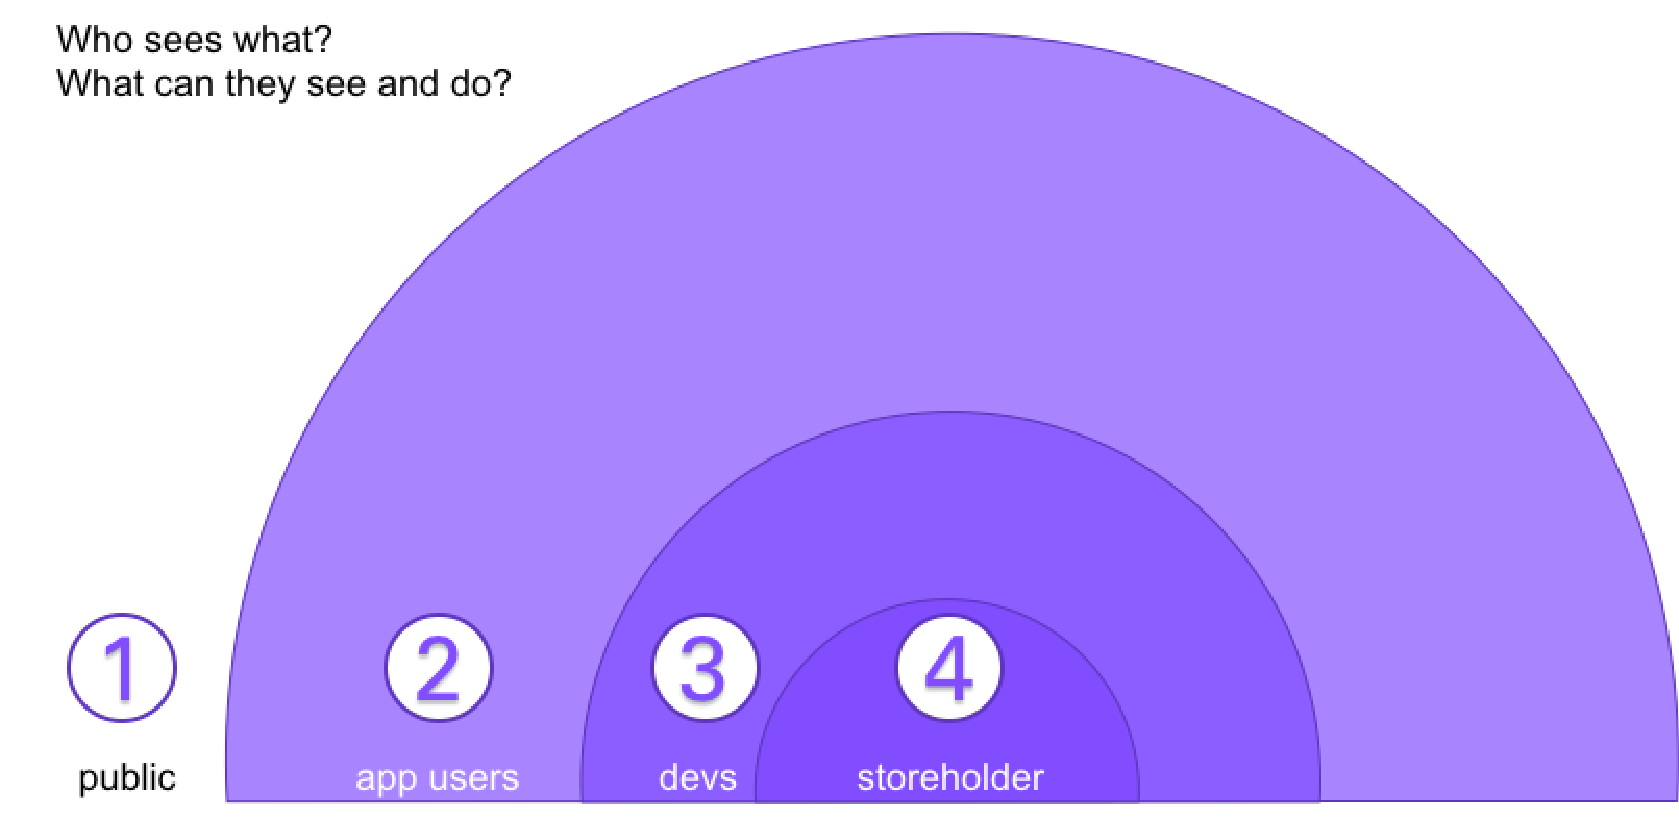
\includegraphics[width=\linewidth]{images/my/who-sees-what.pdf}
    \caption{Four Views of an App Store}
    \label{fig:4-views-of-apps-in-app-store}
\end{figure*}

Figure~\ref{fig:4-views-of-apps-in-app-store} illustrates the four views; broadly, those closer to the centre can also see what those in outer rings can see. As a wise supervisor commented: \emph{``It's a bit like standing at different elevations on a mountainside and looking out over the landscape - the higher you are, the more you can see"}.

The first view is the public view of the app store, what is visible to someone who is not actively engaged with the app store. Examples include people who are not logged into their account, search engines, researchers mining the app store for ratings and reviews, and so on. The public is able to see aggregate ratings and some recent reviews for specific apps. Older reviews are generally hidden from public view (which may limit some research and search engine insights).

The next view is that of a user of a particular app or set of apps. They may have installed some of the apps directly, they are likely to also have pre-installed apps on their device too. They have the ability to interact with the app store, for instance they can see, create, and update their ratings and reviews~\sidenote{If supported by the app store, for instance Google Play does.}. They can also see the public view.

%\akb{In the sentence below, does '.. records about their interactions ...' refer to the interactions of the developer or the user?}
Developers have the next view, which includes information the app store records about the developer's interactions with the app store, and information the app store provides the developers directly (\emph{i.e.} generated by the app store and related entities), as well as feedback provided by users via the app store (\emph{e.g.} ratings and reviews). Developers can also see the public view, although they cannot see the entire view of their user-base. However they can see any rating and reviews provided by the users.

%\akb{Do we know why the qualified 'often' is needed in the next sentence? Is this a non-deterministic behaviour of app stores and hence a forewarning of some of the data quality issues in the analytics platforms?}
Authors and developers are the two end points of ratings and reviews. Authors create them and developers receive them and can choose to respond to them, at least in some app stores. %these conversations. 
Importantly, their primary communications goes via the app store, rather than being direct, and aspects of these communications are often public for a period. Authors and developers can see their individual ratings and reviews for much longer periods than presented in the public view. The app store can use the ratings to decide on the quality of the app and their assessment may affect various important facets of the app's existence in the app store. For instance, well rated apps may be promoted and poorly rated apps may be demoted in search results. As Google states~\emph{``Apps whose metrics are higher have greater promotability, which raises their ranking in Google Play Store searches."}~\sidecite{android_vitals_best_practices} Also, poorly rated apps are sometimes subject to additional scrutiny and delays in the release process, as illustrated in Figure~\ref{fig:pocketpaint-to-help-better-protect-users} when the overall rating for a release dropped sufficiently to trigger this change. % The communications and implications will be covered later in this section.

\begin{figure*}
    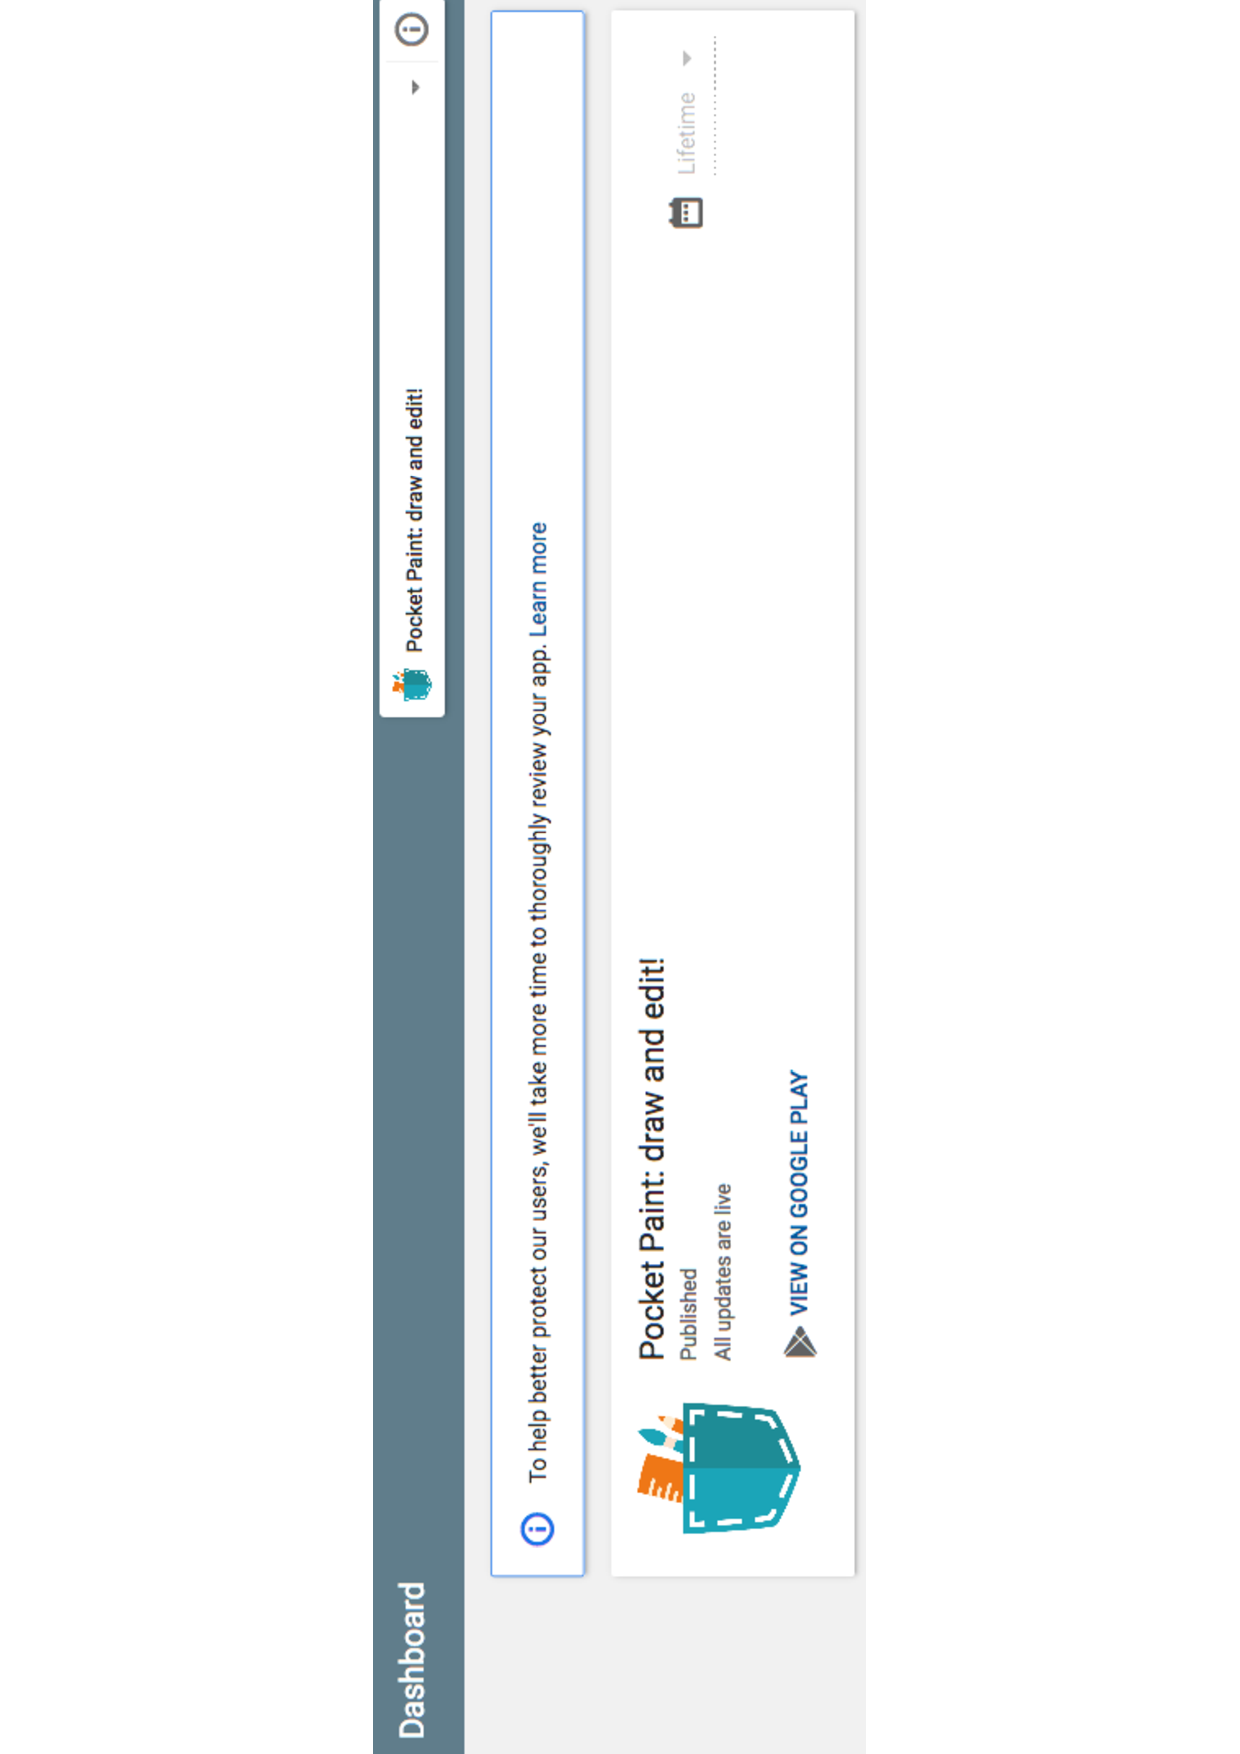
\includegraphics[width=\linewidth]{images/android-vitals-screenshots/catrobat/pocketpaint-to-help-better-protect-users.pdf}
    \caption{Google Play message for Pocket Paint: To help better protect our users...}
    \label{fig:pocketpaint-to-help-better-protect-users}
\end{figure*}

The final view is that of the app store, the `storeholder' in the figure. They have a global and holistic view of the entire store, including \textit{potentially}\sidenote{A caveat on the use of potentially: this is because the app stores are closed systems with limited information about their actual behaviour in the public domain.} all the reviews, user interactions, and whatever usage activities have been performed by all the other three views. 
%\akb{Some explanation of the caveat term 'potential' here would be useful I think - i.e. this is because the app stores are closed systems with limited information about their behaviour in the public domain?}

We now cover various implications of the app store conceptual model.

\subsection{Trust relationships}
One of the key success factors of the modern app store (typified by the Apple App Store and Google Play) was that the platform provider provided the entire ecosystem and established the rules of engagement. The locus of trust is the provider of the app store, which acts as the public face and to some extent also acts as a representative for both the users and the developers. In terms of financial transactions it also acts as the intermediary and facilitates users being able to obtain refunds for app and in-app purchases subject to various conditions. 

Note: There are many details related to the trust relationships for those interested in that topic, however in the interests of focus and concision they are outside the scope of this thesis. 

\subsection{Communications paths and data flows}
There are numerous communication paths for mobile apps both with and without an app store being involved. As the vast majority of apps and users use devices and apps that are part of an app store ecosystem (even if they are obtained from other sources, e.g. as often occurs in India) I will only consider the ecosystem that includes an app store in this thesis. Figure~\ref{fig:sources-of-info-with-app-store-background-ch} illustrates various sources of information for apps available in an app store. The sources and communications paths will be considered next. 
% SHOULD-DO Perhaps a Venn diagram would also complement this illustration?

\begin{figure*}
    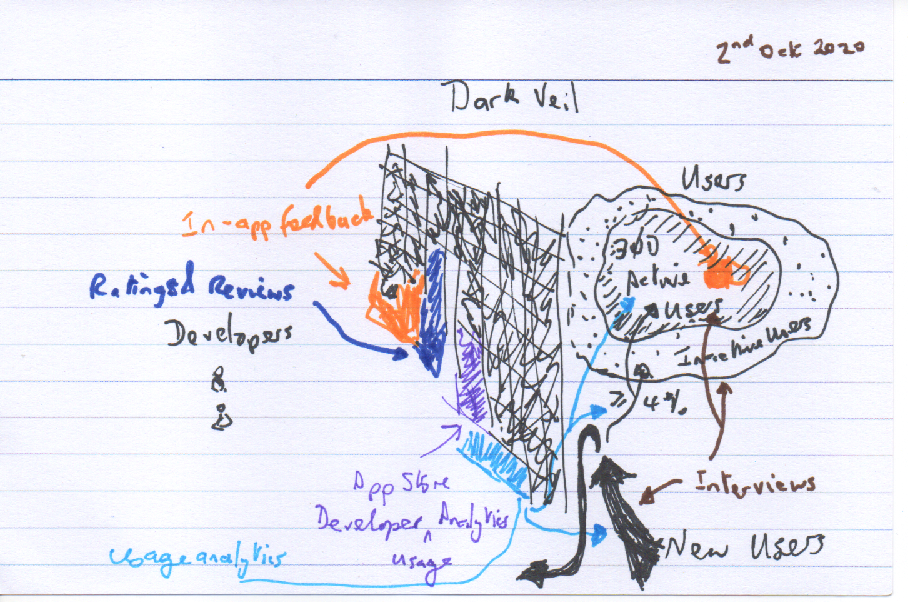
\includegraphics[width=\linewidth]{images/rough-sketches/sources-of-information-with-app-store-1.pdf}
    \caption{Sources of information with an App Store}
    \label{fig:sources-of-info-with-app-store-background-ch}
\end{figure*}

The information about mobile apps can come from users directly or indirectly, from the app if it collects information either directly or indirectly, from devices. Such data collection could be via the operating system, installed apps with privileges to access information about other apps, from accessibility services, and potentially other means e.g. installed viruses. Alternatively, it could come from intermediaries - particularly the app store, and also from network traffic, observers,~\emph{etc.} 

Source code and source code repositories are also useful sources of information about mobile apps. Information can be usefully combined from several sources, for instance from source code about calls to write log messages compared to actual logs recorded when the app has been used on a device. Given the app store plays a pivotal role let's consider its role in terms of communication paths now. 

An app store is more than the store front, it controls and affects many aspects of the ecosystem that gathers around it. It is also more than the software, data and information that the various memberships can access. For instance the modern app stores often include software that is mandatory and pre-installed on end-user devices where that software cannot be easily removed or disabled by users\sidenote{competent, technically savvy individuals may be able to thwart protection mechanisms as may other specialist organisations and software.} . This software includes a local storefront that offers end-users new apps, updates, and enables users to manage optional apps\sidenote{Optional apps can be installed and uninstalled by end users at will. Non-optional apps are installed by various organisations, including the app store provider, some device manufacturers, and so on.}.

The app store provides various primary communications paths between the various parties involved in the ecosystem. It may be an active party, for instance in some of the reports provided to developers and/or users, and in policy-related matters; or it manages communications between app users and developers. Often the app store's owners define the rules of communications, including details such as whether and when apps can ask users to rate an app.

\begin{figure*}
    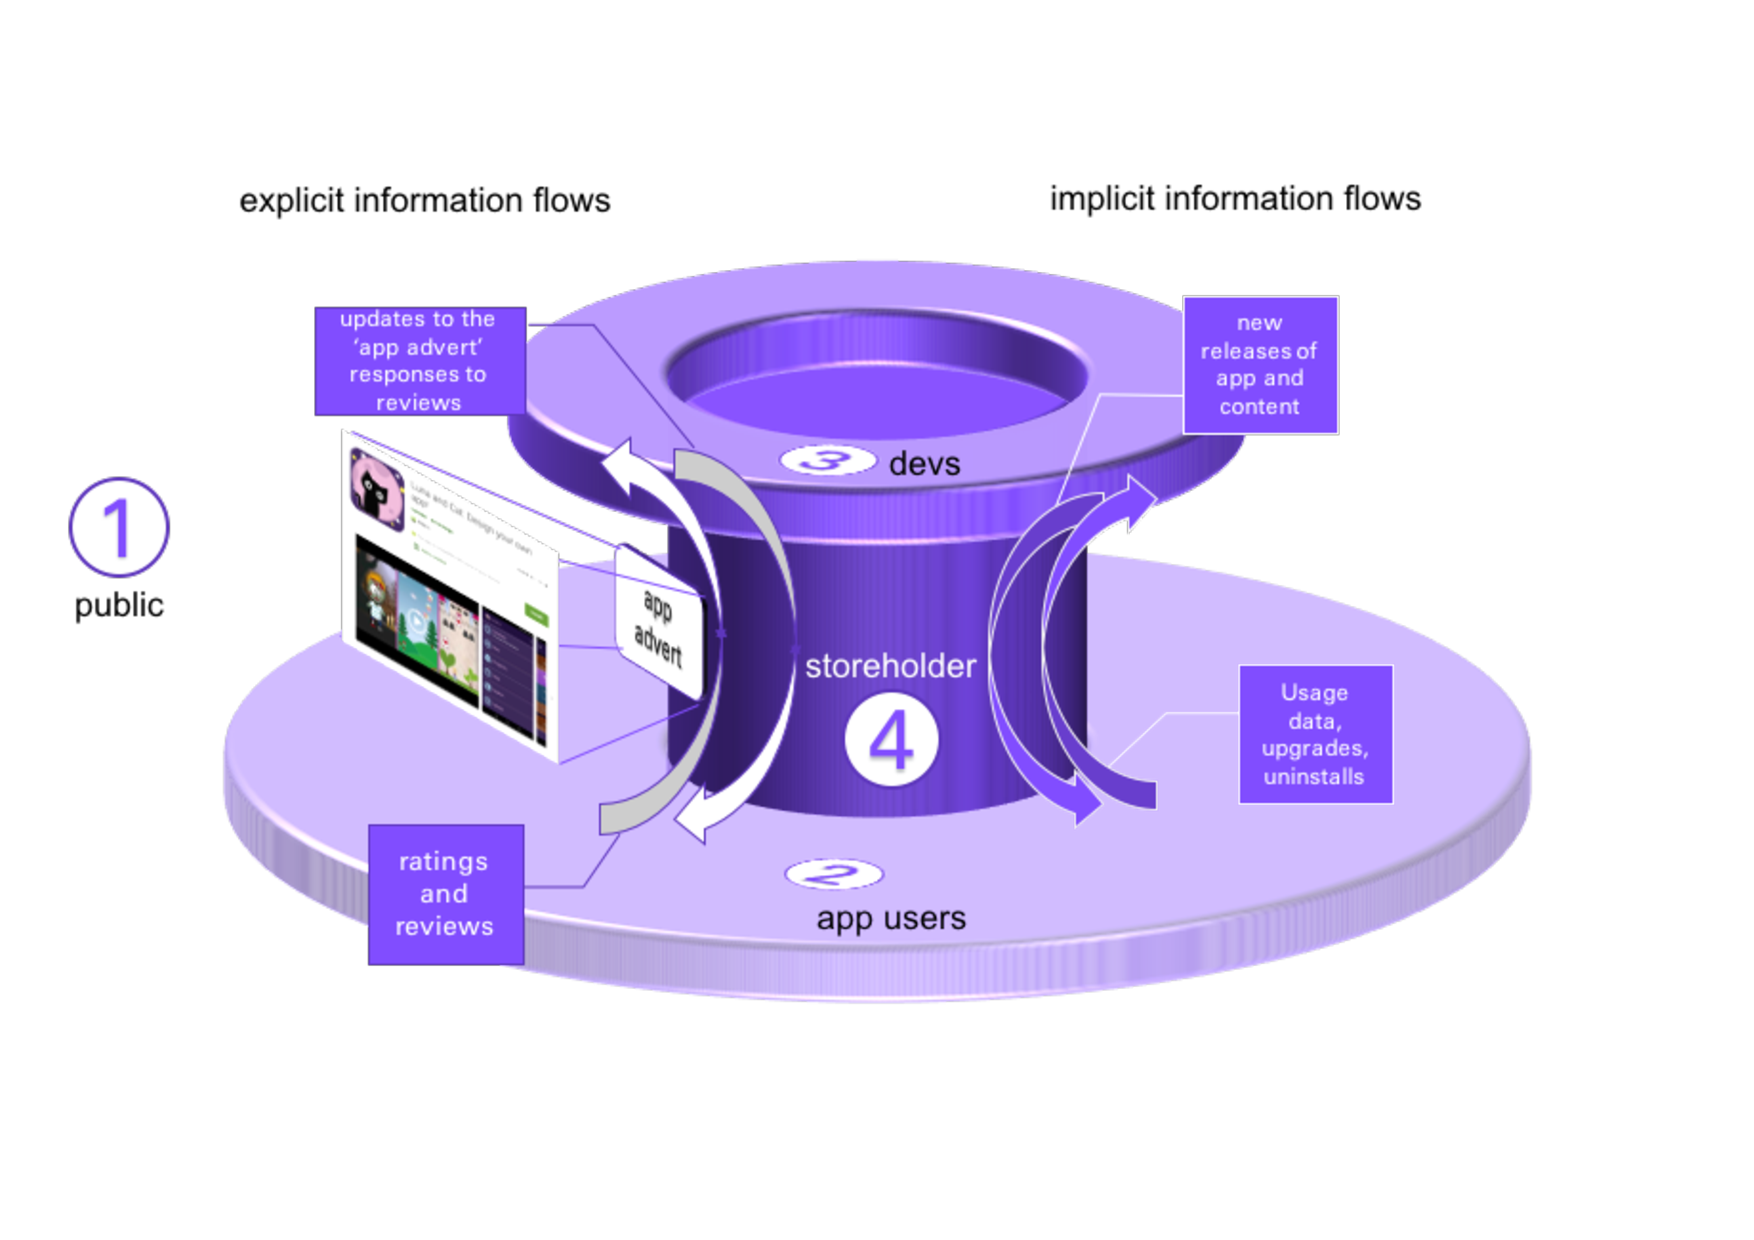
\includegraphics[width=\linewidth]{images/my/app-store-data-flows-3d.pdf}
    \caption{App Store: Communications Paths and Data Flows}
    \label{fig:app-store-data-flows}
\end{figure*}

Some of the communications involves humans, or software chatbots masquerading as pseudo-humans intended to behave similarly to how humans would do in similar circumstances, for instance to provide in-app assistance~\sidecite{baez2021_chatbot_integrations} and to help developers respond automatically to app reviews~\sidecite{greenheld2018_automating_developers_responses_to_app_reviews}. Other communications is generated by software, for instance usage and diagnostic data collected by the operating system and related utilities on a mobile device (collectively described as the platform).

%\akb{Why are bots characterised as 'pseudo-humans'?}

The communications paths and data flows in an app store ecosystem are illustrated in Figure~\ref{fig:app-store-data-flows}. There are two forms of data flows: explicit and implicit. Explicit data flows are actively and intentionally performed by one or more of the participants, implicit data flows represents information that can be inferred or gleaned from various actions and inactions.

Examples of actions intended to communicate explicitly include:
\begin{itemize}
    \item Making the app available in the app store; this includes creating screenshots, a description of the app, adding meta data the app store requires and/or requests, \emph{etc.} This information becomes public if the app store approves the app for release.
    \item Ratings and reviews performed by app users. Only a subset of users provide these, the percentage varies from zero to a maximum of around 10\% with typical percentages around 1\% to 3\%. % SHOULD-DO find credible source for these estimates, I've checked various sources without success
    Estimates vary, partly as the definitions vary too. AppBrain states 46.5\% of Android apps do not have a rating~\sidenote{Their definition is \emph{``Apps that have less than 3 ratings we consider to not have a rating yet"}~\url{https://www.appbrain.com/stats/android-app-ratings}}. In comparison, 42matters.com estimate 41\% of Android apps and 57\% of iOS apps have no rating~\sidenote{\url{https://42matters.com/stats}}.
    \item Responses to reviews, for example Google Play allows developers to respond to reviews, and for both reviewers and developers to update their reviews and responses.
    \item Suspending an app so it is no longer available to users to download. Storeholders sometimes suspend apps and even developer accounts where they perceive the app and possibly the developer contravenes the app store's policy. % c.f. the recent ban of Fortnite in both Apple and Google stores. And see the comment after this article re German law https://www.overpass.co.uk/google-play-account-suspended/ 
    %\href{https://www.ape-apps.com/viewpage.php?p=34186}{My Colony Suspended from Google Play}
    %\href{https://www.ape-apps.com/viewpage.php?p=34173}{My Colony removed from Google Playstore} - over 50% of users come from Google Play.
    
\end{itemize}
%%%%%%% Various interesting sources of Android- (and some iOS) related stats
% https://www.businessofapps.com/data/app-statistics/
% https://www.statista.com/statistics/266217/customer-ratings-of-android-applications/ (seems to be a rehash of AppBrain's report)
% https://mindsea.com/app-stats/
% 

%\akb{Use consistent labels for concepts - below you refer to '(implicit) information flows' whereas above you use '(explicit) actions intended to communicate'.  By using different labels you are suggesting that these two implicit/explicit categories are not directly comparable, i.e., they are different types of things altogether. However, I am not sure this is your intent.}

Implicit information flows include:
\begin{itemize}
    \item New releases of apps and related content (such as in-app content, often purchased using in-app purchasing). These indicate the developer is wishes to actively engage their userbase. Upgrades may include changes to the app seeded by various sources such as ratings and reviews and other data, including:
    \item Usage data and upgrades, both imply the software provides some value to the users. Lack of usage may also be an indication the software is not currently providing value - this may be expected for instance with seasonal apps. Uninstalls are a stronger signal that users no longer see sufficient value in the app to keep it on their device.
\end{itemize}

On-device bug reports may be a hybrid, where the bug reporting utility on the device does much of the data collection and may report this automatically and transparently, however it may sometimes ask the user for additional input and permission to send the bug report.

\subsection{Membership criteria of each group}
%\akb{Explain why the membership criteria are important to understand, perhaps combine with next section single explanation of groups and what members can do in each}
As Figure~\ref{fig:app-store-data-flows} illustrates there are four numbered groups in the illustration. People can potentially belong to more than one group (albeit membership of the storeholders is limited to owners and those they assign membership to,~\emph{e.g.} as administrators of the app store). Group membership constrains what the members can do as participants and what they have access to.

\begin{enumerate}
    \item Public: the membership criteria are minimal. Here `public' is any entity, human or technological, that has access to the app store\sidenote{For our purposes we can assume online digital access, other modes may also be viable, for instance some researchers use archives of data sourced from app stores.}. An example of a technological entity, is a search engine crawler or software including web scraper technology and scripts that use APIs provided to obtain information about apps in the app store.
    %\akb{Not sure what is meant by 'minimal' here. You could describe 'public' as any entity, human or technological, that has access to the app store. Provide an example of a technological entity, e.g., a search engine crawler}
    \item App user: the public can use an existing account or create a new account with the app store that would allow them to become an app user~\sidenote{They need to meet the criteria of the app store.}. Note: there may be restrictions or constraints that mean not everyone can install every app on every device, however the general practice is that apps are freely available for app store users to install on any device they possess. 
    \item Developer: developers need to be registered and validated by the app store, the process varies for specific app stores, they often involve payment of a fee and some amount of validating their identity. Some app stores may perform additional checks based on information they and/or others hold.  
    \item Storeholder: they are generally a legal entity, and certainly for the purposes of this research they are. Apart from a few exceptions (such as F-Droid~\sidenote{Details are available online at~\url{https://www.f-droid.org/en/about/}}) they are multi-national major corporations.
\end{enumerate}


\subsection{What participants can and cannot do (and who dictates the rules?)}
%\akb{You don't explain the link between the implicit/explicit data flows and these membership groups.}
\begin{itemize}
    \item Public: The public cannot review an app or easily download the app. They can view publicly accessible information, including information that was gathered previously, potentially by others.
    \item App user: They can rate and review apps they have installed on their account~\sidenote{ user may have several devices and choose not to install an app on all of them. Also some apps may by limited to devices that meet particular criteria e.g. the platform version.} or device. They can also install, update and deinstall apps~\sidenote{There may be restrictions imposed for some apps, for instance Google Apps and Manufacturer apps might be blocked from being uninstalled, and updates are sometimes mandatory, \emph{etc.}}.
    \item Developer:  Approved developers can upload apps to the app store and publish them if the app store also approves the release. They can choose to submit new versions of their apps, sometimes they may be required to do so by the app store. They can choose to suspend or withdraw their app from the store, note: generally users can continue to use the app if they have it installed. Developers are expected to interact with the app store and often do so of their own volition, for instance to see how their app is `doing'. The developer may define a price for their app and/or any in-app purchases. They may also require users comply with additional terms of use, and many apps do so.
    \item Storeholder: They are by far the most powerful participant as they establish the ecosystem including the rules of engagement and enforce these rules. The app store has the right of delay or veto of releases, it can suspend apps and developers, and much else besides. They are expected to comply with the laws of the various countries the app store is available in and also where their business is situated. These laws may affect the developers and the app users, for instance the amount of sales tax charged on a purchase in the app store.
\end{itemize}

We have already identified four membership groups involved in app store ecosystems, there is at least one more and also additional data flows in the ecosystem. The fifth membership group is a~\emph{service provider}. These service providers provide non-trivial functionality and other capabilities such as in-app analytics, feedback, and so on. Developers can choose to incorporate software libraries into their apps and use the services provided, for instance as conduits of communications between the app and the developers. Here developers include other specialist groups in their organisation such as customer service personnel and marketing teams. Many app developers choose to use at least one such service, some incorporate several and there is even specialist software that enables developers to manage multiple similar services within their apps on end-user devices. An example of this type of software is~\url{https://github.com/segmentio/analytics-android} (other platforms are also supported and there are other providers of similar software).

Membership matters in particular because of who has access to which data and for how long they have access. Note: Control and `ownership' of the data are also relevant topics, however they are not necessary to comprehend the rest of this topic. % SHOULD-DO consider whether to add material on this topic in the thesis. 

\subsection{Phases of a release}


\begin{figure*}
    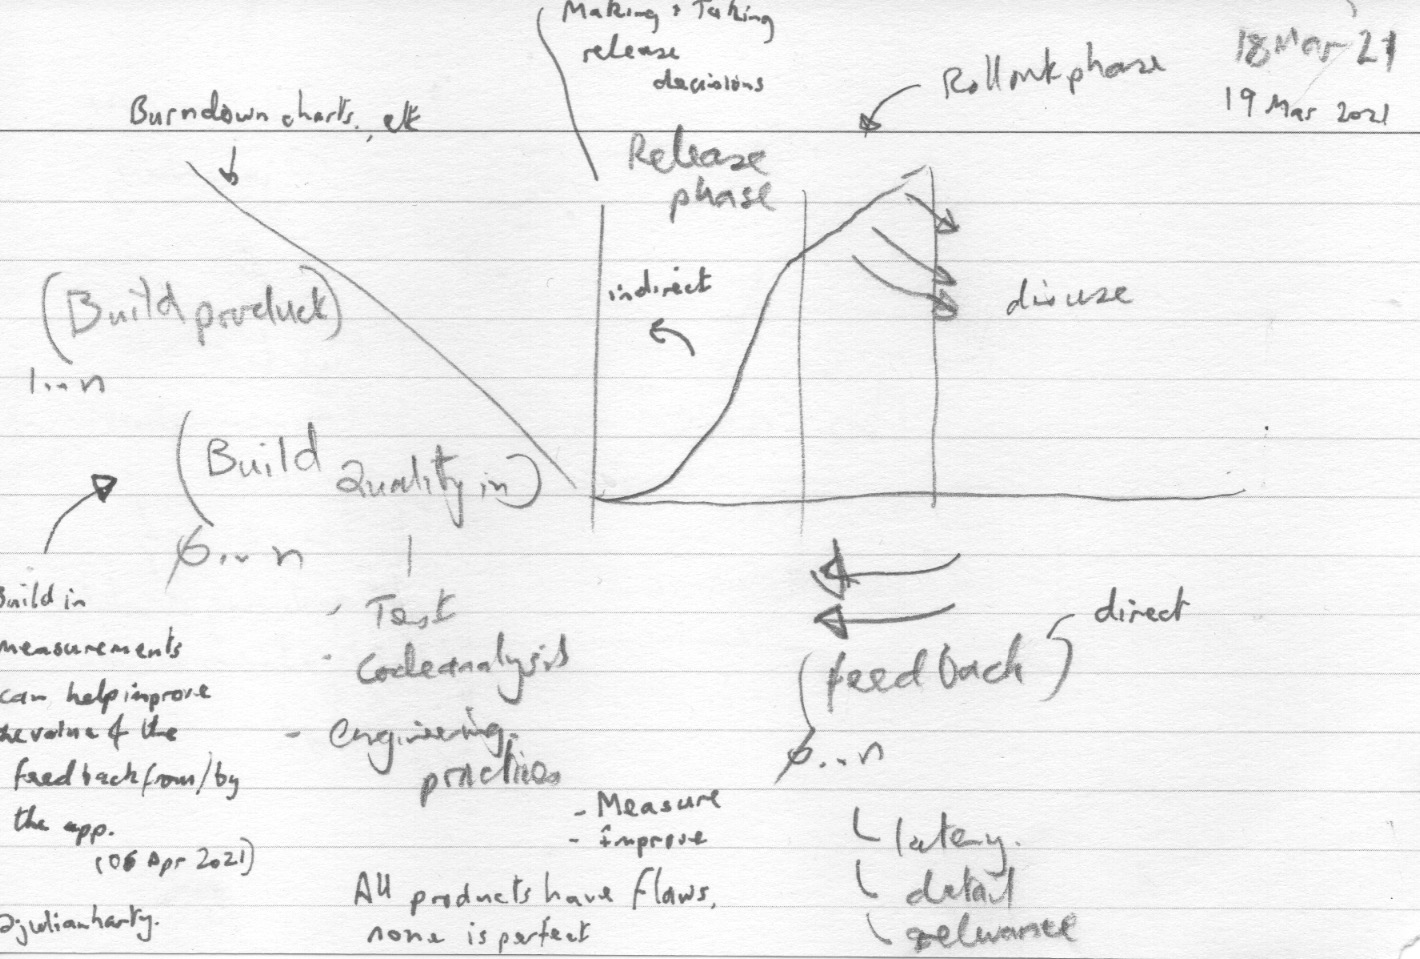
\includegraphics[width=\linewidth]{images/rough-sketches/Red-Thread-Rough-Sketch.jpeg}
    \caption{The lifecycle of a release and where mobile analytics provides feedback}
    \label{fig:red-thread-for-this-thesis}
\end{figure*}

For any given release of a mobile app there are at least three material phases in order for the release to be used:
\begin{enumerate}
    \item Building the product: which may incorporate practices and tools intended to ship a `quality product'. Some teams also incorporate logging and reporting to help measure the behaviours of the app in use, post release.
    \item The Release: For some projects this may be as simple as uploading a new binary and making it fully available. For others they may incorporate decisions and mechanisms to make each release with the aim of de-risking any undesirable/adverse effects of the new release.
    \item Deployment: Deployment occurs when end users install and start using the release of the app. Both the app store and the end users affect when this occurs. App developers can try to hasten when users install the latest release through various mechanisms, for instance through implementing and mandating users upgrade their current release.
\end{enumerate}

Figure~\ref{fig:red-thread-for-this-thesis} illustrates these three phases together with some of the dynamics \emph{e.g.} of rollout and disuse of a release, and of feedback from whatever sources that the development teams can choose to pay attention to and apply. These phases are part of a longer lifespan of the release that includes an often long-term postdelivery period~\sidecite[][pp 156-157]{evans2004_achieving_software_quality_through_teamwork} where users use the release until it is decommissioned or replaced with a subsequent release.

\begin{figure*}
    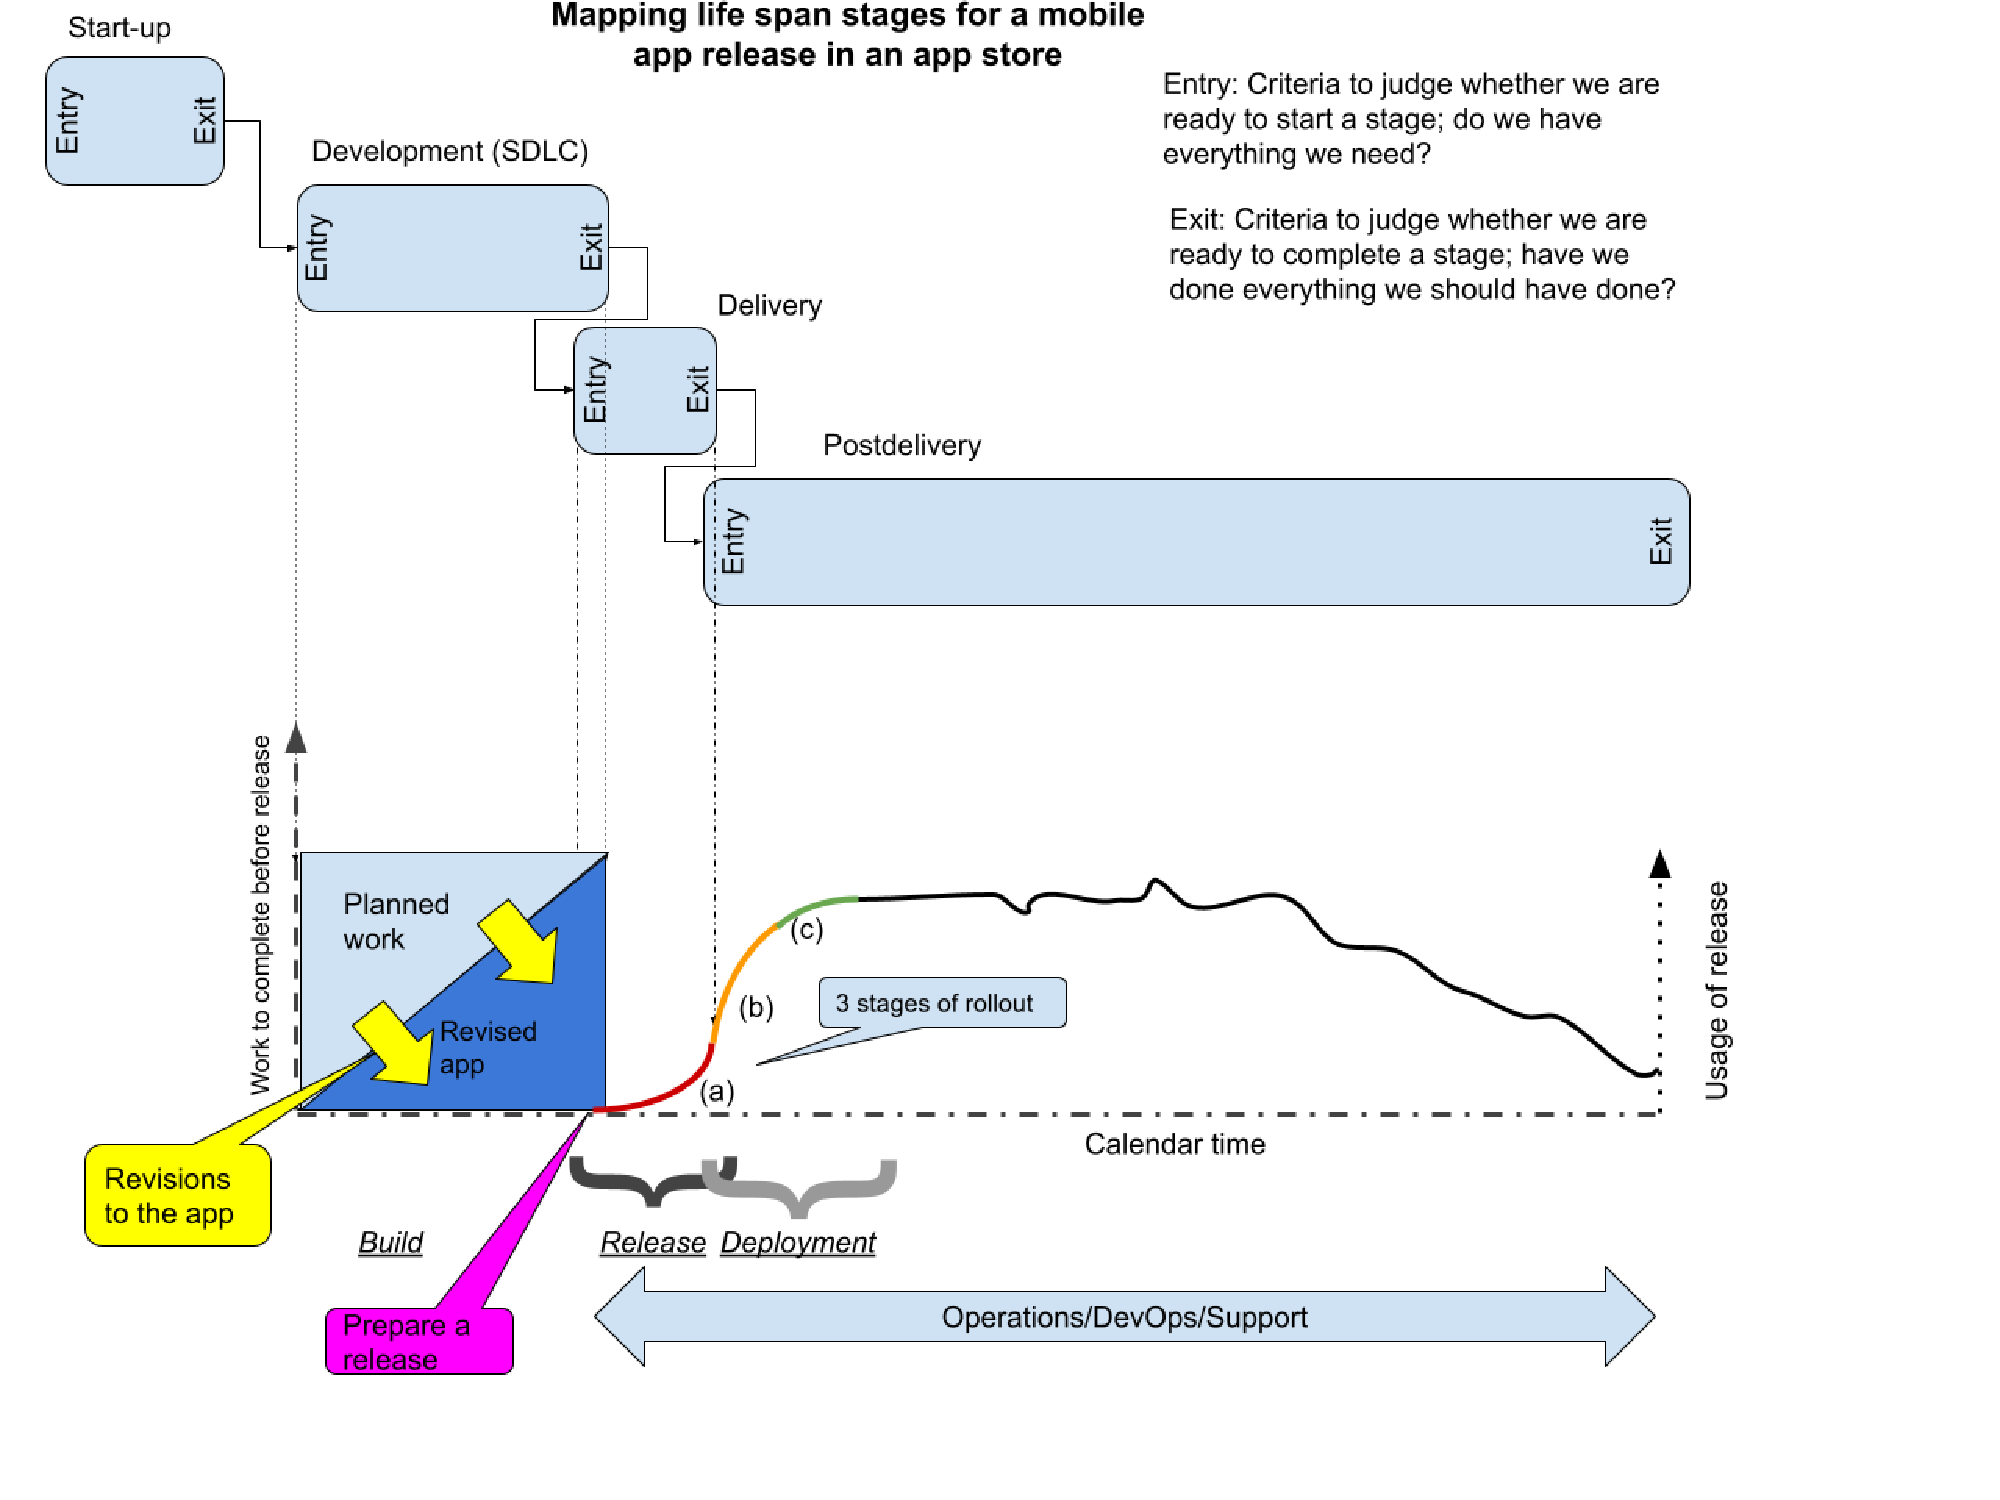
\includegraphics[width=\linewidth]{images/my/mobile-app-life-span-stages-21-sep-2021.pdf}
    \caption{Mapping life span stages for a mobile app release in an app store}
    \label{fig:mobile-app-life-span-stages}
\end{figure*}

Figure~\ref{fig:mobile-app-life-span-stages}~\sidenote{Source of figure, Google Drive file: \href{https://docs.google.com/document/d/1d4B5l1tlpclHdKwY8W00qchiCV2YK5JjJP8TbkRHcjQ/edit}{Mobile app life span stages}.} compares a revised version of the `Life span stages' Figure in~\sidecite[][p.155]{evans2004_achieving_software_quality_through_teamwork} mapped approximately to the three stages first illustrated in Figure~\ref{fig:red-thread-for-this-thesis}. Mobile app releases in an app store extend the Delivery which may also overlap either or both the development and the postdelivery life span stages. The overlap with the development stage is because the development is not complete until the app store accepts/approves the release (this may include pre-launch checks, automated testing, and so on depending on the app store). The overlap with deployment happens as releases are often released incrementally initially to a small percentage of the userbase - at least some of the users in that percentage will install the new release, until the percentage has been achieved. Meanwhile at least some of those users will use the app which will then mean the release is operational and may need operational support.


\section{Conceptual model of layers within apps and observation points}
Observation can be internal,~\emph{i.e.} built into apps, and external. External includes instrumentation, debugging tools, the operating system at runtime, accessibility interfaces, event listeners, log watchers, and so on (as this is not intended to be an exhaustive list). The observation may also be indirect, for instance using network monitoring software, and/or from remote APIs, REST endpoints, and web servers (with their attendant logging).

\subsection{Three layers of an app}
In earlier work, published in ~\sidecite{harty_aymer_playbook_2016}, the concept of three layers of an app was introduced. These are illustrated in Figure \ref{fig:3-layers} and shows three primary conceptual layers related to a mobile app. 


\begin{figure*}
    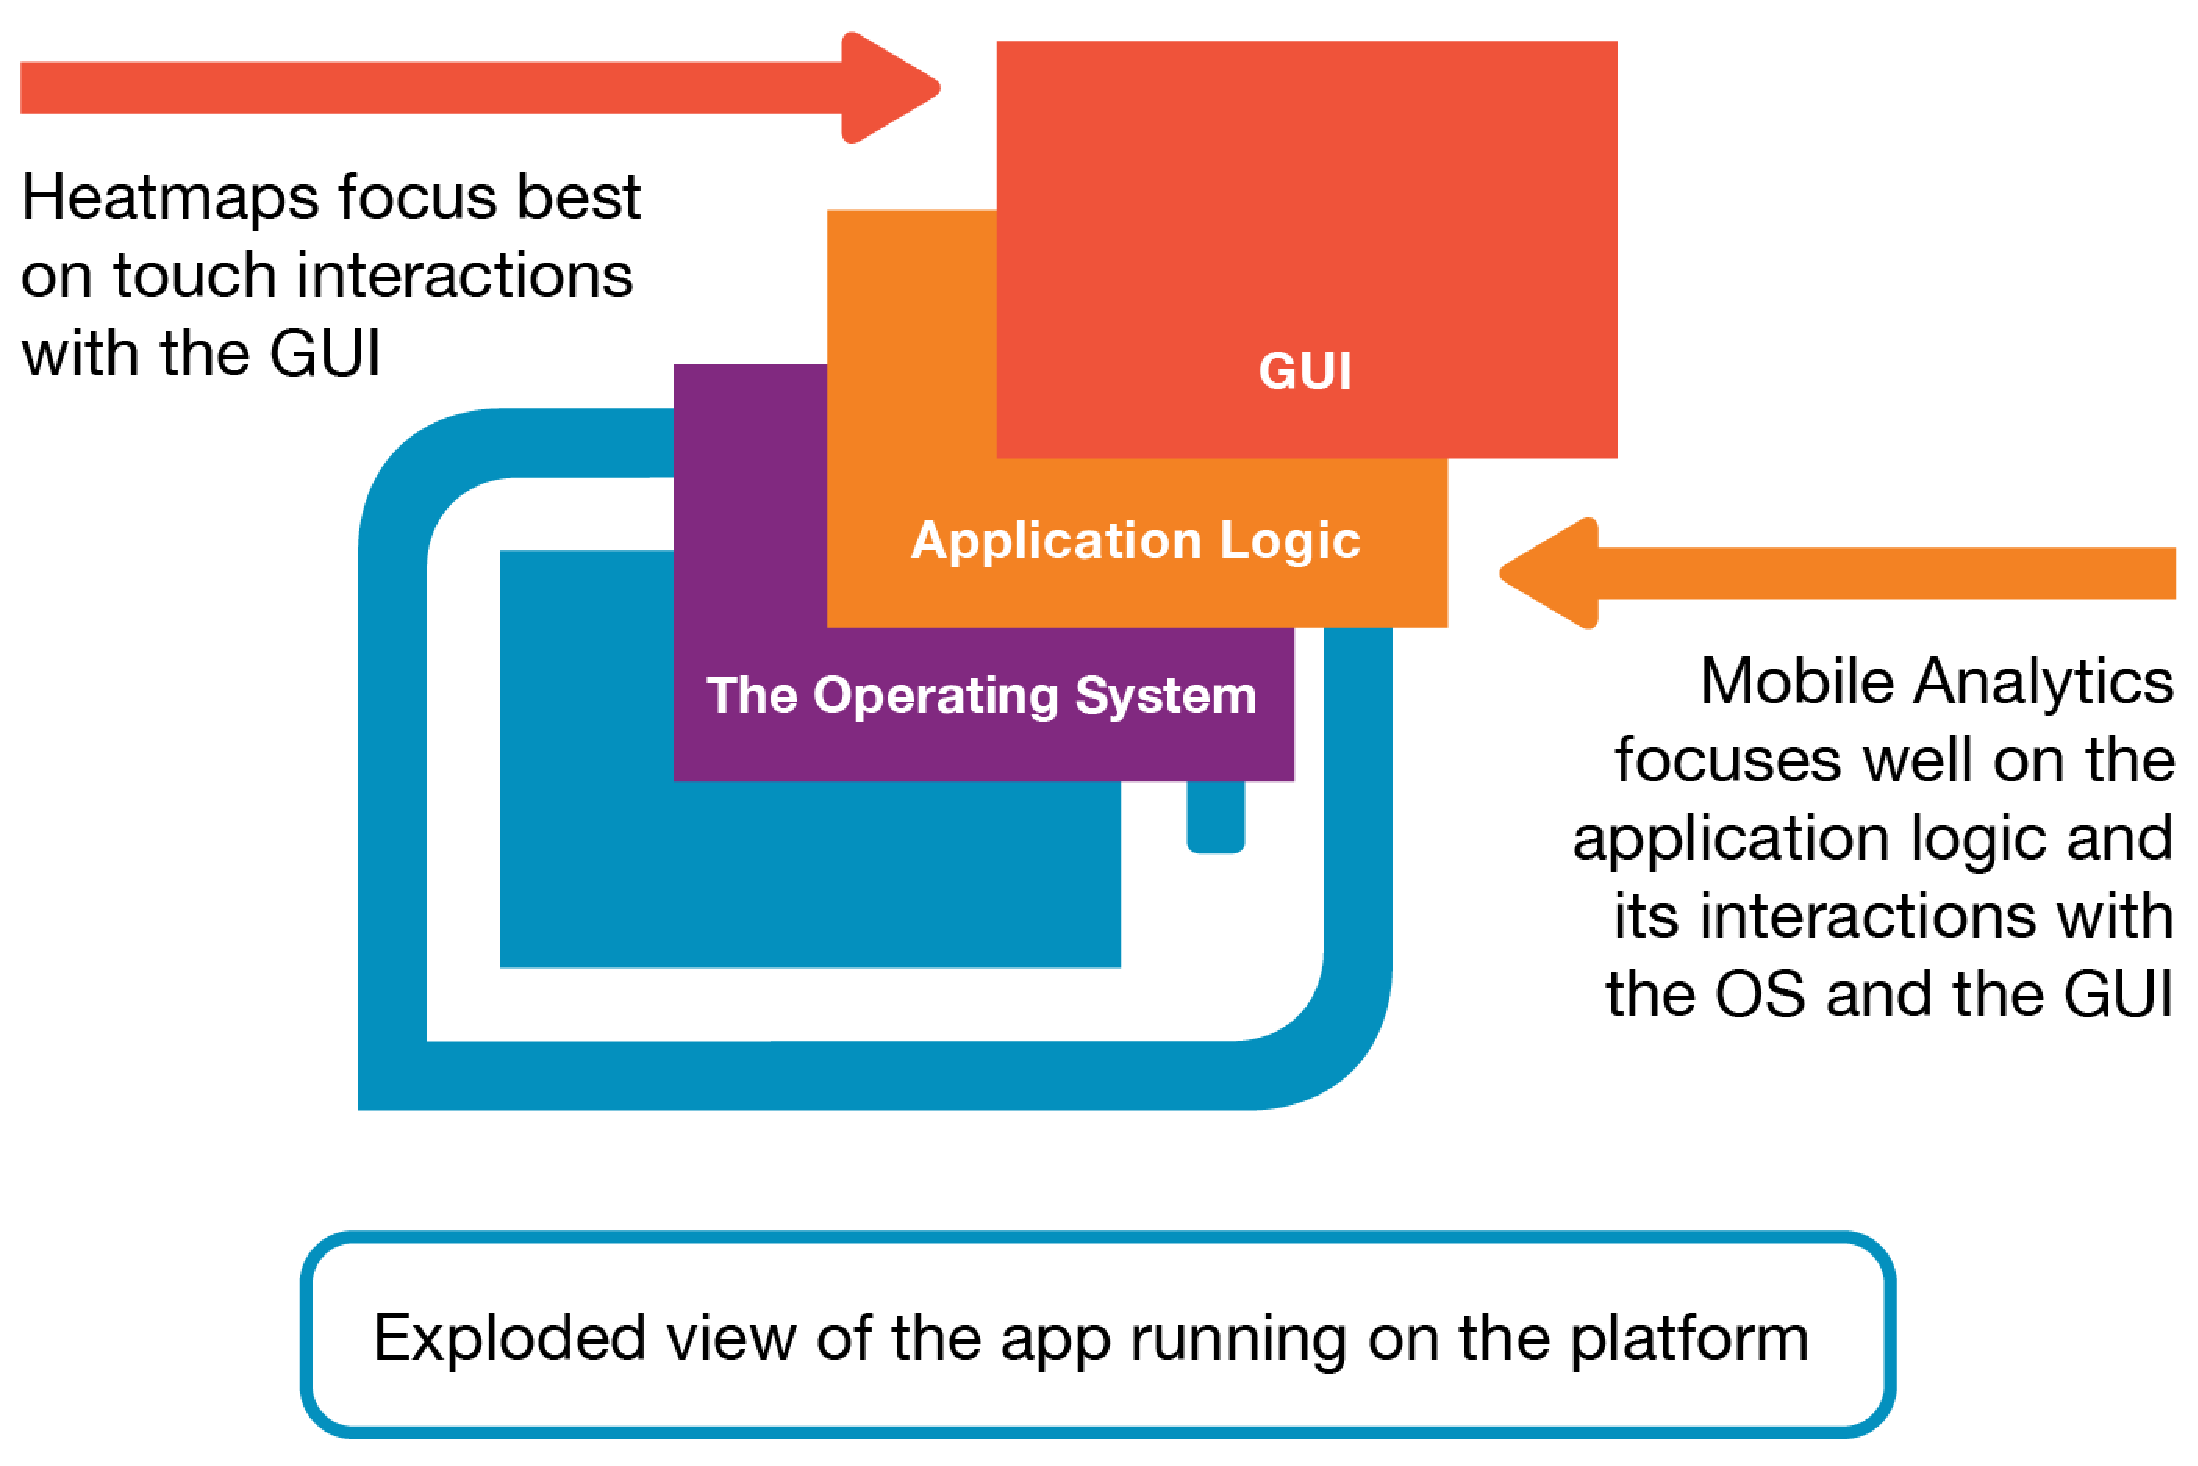
\includegraphics[width=\linewidth]{images/mobile-analytics-playbook/3-layers.pdf}
    \caption[Three layers of an app]{Three layers of an app {Image credit: First published in The Mobile Analytics Playbook~\cite{harty_aymer_playbook_2016}}.}
    \label{fig:3-layers}
\end{figure*}

Of course, apps aren't quite this simple or well defined in reality, for instance they include software libraries from various sources, A/B testing utilities, logging code, run-time lifecycle management, and so on. Nonetheless, these three layers are a useful abstract, particularly in terms of useful observation points about apps on user's computer devices~\sidenote{Another observation point that was orthogonal to the application logic layer was one popularised by a company that has since been acquired, called SafeDK. They provided app developers with software that provided an interface between the developer's code and the libraries the code used. This software collected and reported usage data on the performance and reliability of the libraries. Given the commercial nature of the business, their acquisition and the demise of their products and the company's website, and the fast moving nature of the internet, obtaining concrete information may be impractical for all but a few people who know those who were involved at the time.}.

The \Gls{gui} can be visually observed by sighted users, it can also be observed by Accessibility software, and test automation tools, \emph{etc.} externally to the app. It can also be observed from within the app, for instance through using software known as \emph{heatmapping} that records the screens and the touch interactions performed by users of that screen. One of the the more popular, mature heatmapping offerings is from AppSee~\sidenote{\href{  https://www.appbrain.com/stats/libraries/details/appsee/appsee}{AppBrain stats for AppSee}. Note: in 2019 Appsee's team was ~\href{https://techcrunch.com/2019/05/13/servicenow-acquihires-mobile-analytics-startup-appsee/}{acqui-hired by ServiceNow} and the service no longer directly available.}, nonetheless they are only used in a small minority of mobile apps.


\subsection{Observation points: inside-outside perspectives}
The observation point determines what can be observed and how. 
As Figure~\ref{fig:internal-external-table} illustrates there are internal and external perspectives on an app for various purposes, including observations, interactions (e.g. through test automation), and emitting information (e.g. through logging, reporting, or mobile analytics). Where the information is observed affects what can be known and what is possible, an insider is privy to information an outsider is not; whereas an outsider has perspective and can potentially perceive things insiders cannot.


\begin{figure*}
    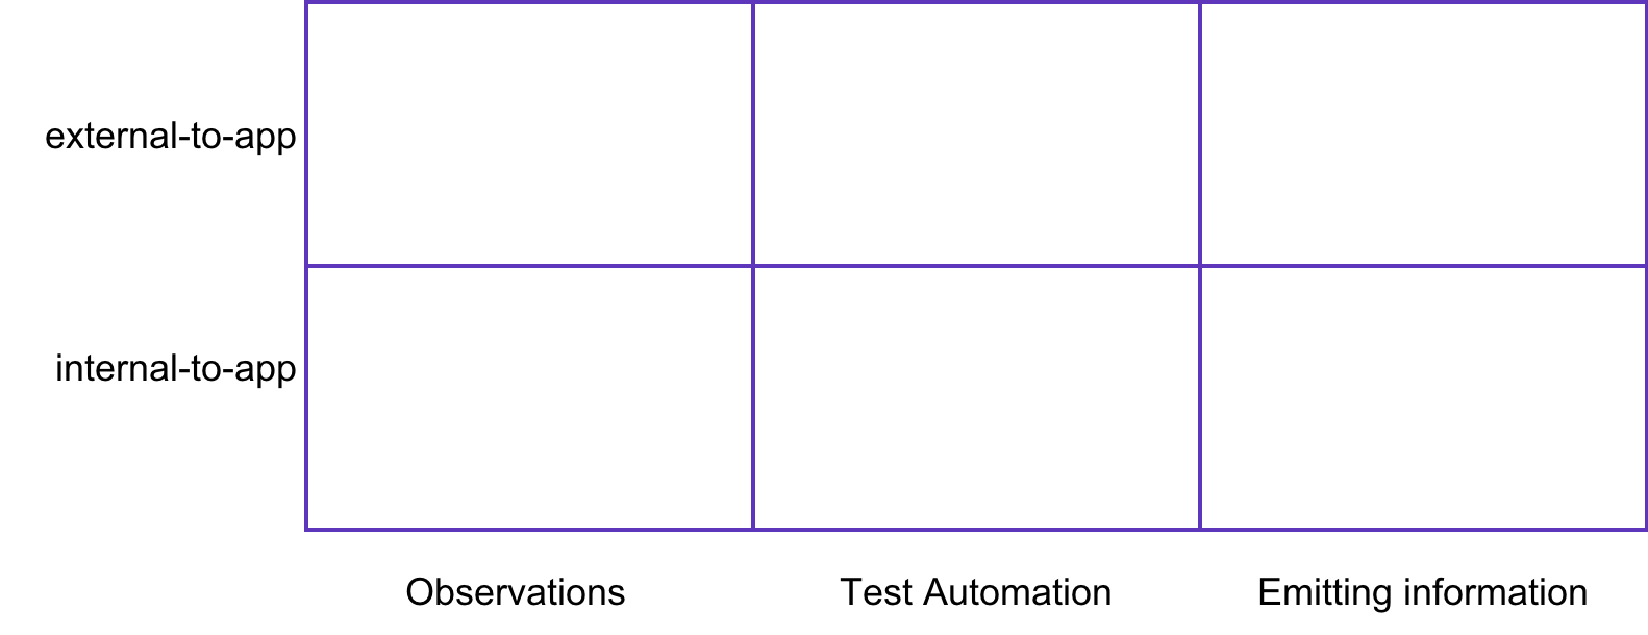
\includegraphics[width=\linewidth]{images/internal-external-table.pdf}
    \caption{Internal and external perspectives of an app}
    \label{fig:internal-external-table}
\end{figure*}

%\textbf{SHOULD-DO} Expand the following: What is test automation? discuss how mobile apps are tested, the unique aspects of using accessibility interfaces, etc.


\section{Conceptual model of analogue and digital feedback}~\label{analogue-and-digital-feedback}
Feedback can help developers to find and choose ways to improve their software. Various researchers have investigated way to understand and use feedback provided by end-users, for instance, in ratings and reviews users provide to the app store. For the purposes of this research feedback people provides is considered~\emph{analogue feedback} as it has the richness and complexity of analogue signals, and also challenges of processing and comprehension.

In contrast, digital feedback originates from software and is generally deterministic~\sidenote{~\url{https://en.wiktionary.org/wiki/deterministic}}. For the purposes of this research~\emph{digital feedback} is provided by running software where programmers added code to programs to collect data that provides feedback about software use and certain behaviours of that software. The addition of the code may be automated, in part, or wholly, for instance by another program or script. As an example, AppPulse Mobile claims they can add analytics automatically without developers writing a line of code~\sidenote{~\url{https://www.microfocus.com/en-us/products/apppulse-mobile-app-apm-monitoring/overview}}.

\begin{figure*}
    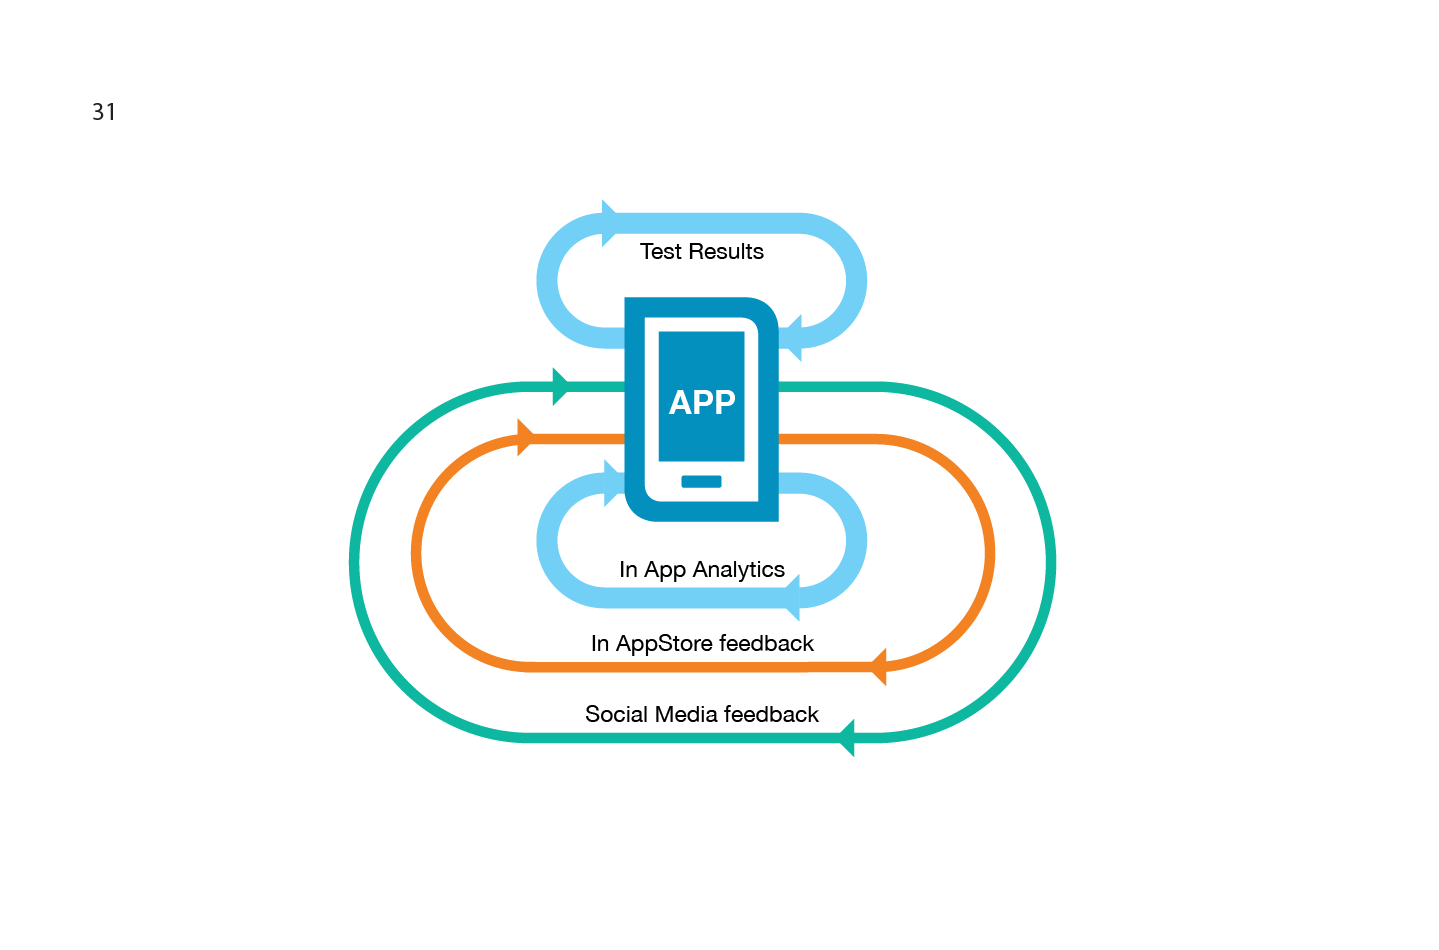
\includegraphics[width=\linewidth]{images/mobile-analytics-playbook/Chart-07-FeedbackLoops.pdf}
    \caption{Feedback Loops for mobile apps~\cite{harty_aymer_playbook_2016}}
    \label{fig:map2015-feedback-loops-for-mobile-apps}
\end{figure*}
%SHOULD-DO edit the figure to remove whitespace, etc.

Figure~\ref{fig:map2015-feedback-loops-for-mobile-apps} illustrates various feedback loops where the feedback could be used to change and improve a mobile app. Within the team's aegis are test results (and static analysis, etc.). Beyond their direct control are feedback within the app, within the app store, and outside the app store ecosystem such as feedback on social media about their app. This figure illustrates in-app analytics which was the primary form of analytics at the time the figure was published, since then two additional forms of feedback have emerged: platform-level feedback such as Android Vitals and in-app feedback.

\subsection{Analogue feedback: in-app tools}
One source of feedback is when apps include feedback mechanisms within the app. Various benefits are touted to encourage developers to add such feedback including the ability to: ~\emph{``...capture valuable insights into the usability of the app and quickly resolve any issues..."}~\sidecite{mopinion2017_top11_mobile_in_app_feedback_tools}, for example. 

Some apps also collect in-app feedback if the user indicates they are not satisfied with the app and conversely ask users to submit a review online in the app store if they are satisfied. One hypothesis is their developers have implemented this approach to divert adverse ratings and reviews from public view and from the app store algorithms. 

In-app feedback enables a wider range of communications and also scope for richer dialogues than relying on feedback mechanisms provided by app stores which consist of a rating and an optional plain text comment. Examples of wider ranges of communications include surveys, and richer dialogues include audio recordings.

In-app feedback has also been proposed for bi-directional communications between developers and users of the app for instance to elicit non-functional requirements~\sidecite{avellis_harty_yu_towards_mobile_twin_peaks}.

\subsection{Analogue feedback: app store feedback}
App store feedback, combines a rating (typically using a one- to five- start rating and an optional plain-text comment). It is a subject covered by significant volumes of research and discussed in the related works chapter. %MUST-DO actually write up this related research and contrast it with mobile analytics.

\begin{figure*} %[!htbp]
    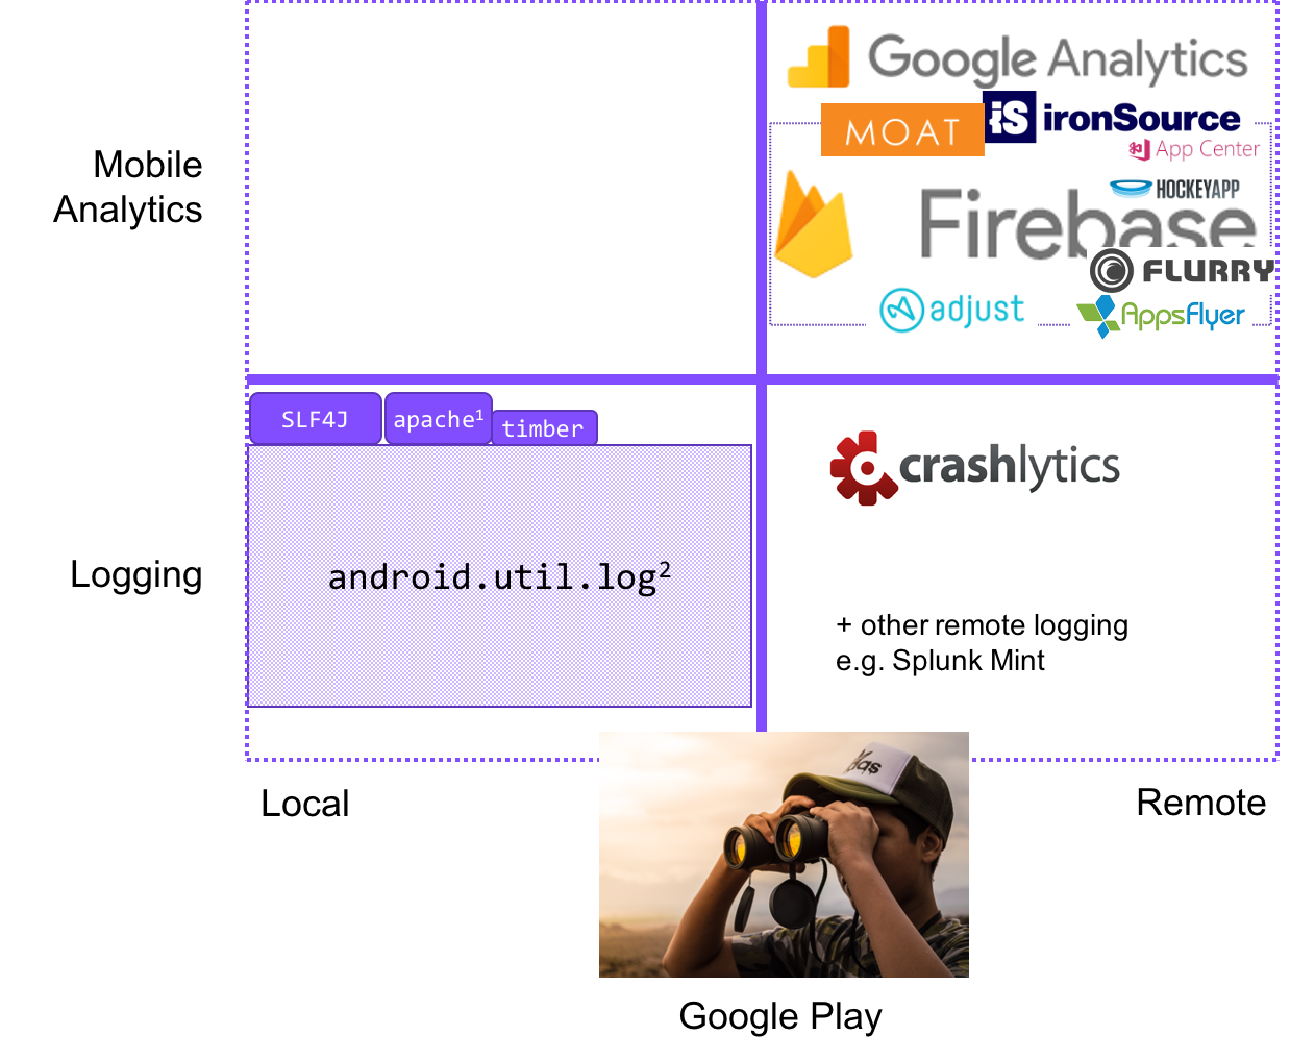
\includegraphics[width=\linewidth]{images/matrix-of-logging.pdf}
    \caption{Matrix of logging}
    \label{fig:matrix-of-logging}
\end{figure*}

\subsection{Digital feedback: logging and mobile analytics}
The application may incorporate logging and/or mobile analytics. Logging in mobile apps is often used locally, by developers independently of other mechanisms. Mobile analytics is used remotely, as are crash reporting libraries. 



Figure \ref{fig:matrix-of-logging} illustrates a matrix of logging, where logging and mobile analytics are on the Y axis and local and remote on the X axis. There is a cross-cutting example where the mobile platform observes local events and then forwards the information remotely. A good example is Google Play which appears to be an external observer of data recorded in device logs. Data collection runs locally and is sent to Google servers where Google analyses the data and provides reports to developers for their apps. %SHOULD-DO check for related US patent filings by Google in this area.

\begin{table} %[!htbp]
    \centering
    \begin{tabular}{lll}
         Category of logging &Local access?  &Remote access? \\
         \hline
         None            &N/A  &N/A \\
         \texttt{StdOut} &It depends &Unlikely \\
         Default platform logging library &Yes &Possible \\
         Enhanced platform logging library &Yes &Possible \\
         Third-party logging library &as-designed &as-designed \\
         Proprietary logging library &as-designed &as-designed \\
         
    \end{tabular}
    \caption{Choices available to developers for logging in mobile apps}
    \label{tab:logging-choices-for-devs}
\end{table}

Table~\ref{tab:logging-choices-for-devs} identifies various categories of logging available to developers of mobile apps. They range from no active logging in the app (some information is still logged by the platform) to proprietary custom logging libraries which a tiny minority of development teams would chose to do - they may do so to keep their logging as private as practical from the rest of the device.

\texttt{StdOut} is often used in code written for other platforms including Linux that has been ported to mobile platforms. Some people who are unfamiliar with logging libraries who have a superficial understanding of developing for mobile devices may also use print statements in their code (which effectively writes to the standard output) rather than use log statements in their code. There are various nuances of how the standard output and standard error outputs are handled in Android code (Java, Kotlin, etc.) and native code (C/C++) are directed as standard for Android apps. In short, for native code (\emph{e.g.} written in C/C++) as standard the outputs are discarded by `writing' them to~\texttt{/dev/null}. For Android code (\emph{e.g.} written in Java/Kotlin) \texttt{System.out} and \texttt{System.err} can be redirected to the log on some Android releases if the device is configured to do so.
%MUST-DO add references for https://github.com/android/ndk/issues/671 and https://codelab.wordpress.com/2014/11/03/how-to-use-standard-output-streams-for-logging-in-android-apps/ and https://stackoverflow.com/a/17199704/340175 and https://stackoverflow.com/questions/10531050/redirect-stdout-to-logcat-in-android-ndk

There are various enhanced log libraries, for instance~\texttt{timber} which are used by discerning app developers. These libraries also write to the platform log files. 

To Be Continued. %MUST-DO

\begin{figure*}
    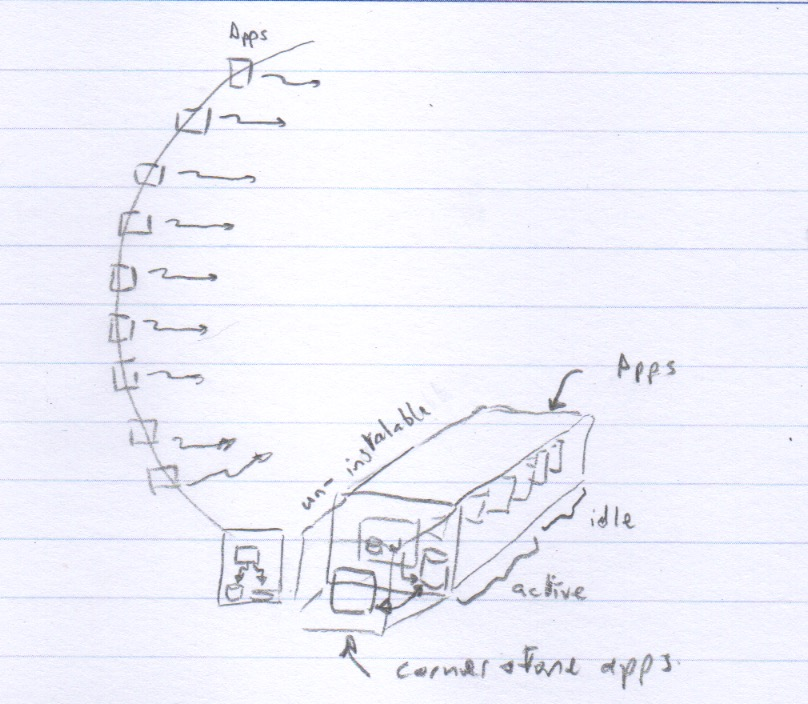
\includegraphics[width=\linewidth]{images/rough-sketches/apps-on-device-boundaries-sketch.jpeg}
    \caption{Apps on the device boundaries}
    \label{fig:apps-on-device-boundaries}
\end{figure*}

\begin{figure*}
    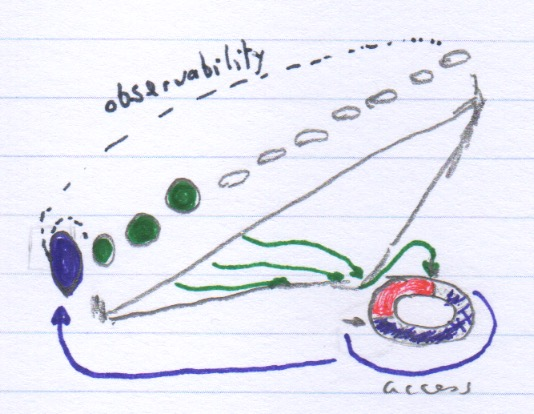
\includegraphics[width=\linewidth]{images/rough-sketches/on-device-logging-sketch.jpeg}
    \caption{On-device logging}
    \label{fig:on-device-logging}
\end{figure*}

A couple of rough sketches, Figures~\ref{fig:apps-on-device-boundaries} and~\ref{fig:on-device-logging} present two views of apps installed on any given mobile device. These apps are broadly one of three categories: platform, pre-installed (non-removable), and user-installed (removable). Here the focus is on their use of logs on the device.

At any point one or more of these apps may be running, the rest are idle. The majority of these apps, with the possible exception of system apps, write to one or more shared, common, log files. These log files have a finite size, and once they are filled newer messages overwrite the oldest ones in turn. In Figure~\ref{fig:on-device-logging} the left-most blob, in purple, represents a system app that is able to read the shared system log files. These apps are pre-installed by the manufacturer, they may include those from the provider of the platform, particularly from Google for Android devices that use Google Play, and also some device manufacturers may have similar apps. Other apps are also pre-installed by manufacturers including a suite of apps from Google and some from the manufacturer. They may also include apps from organisations with agreements with the device manufacturer, for instance they may pre-install some games and utilities from partners. TBC.


As an observation the vast majority of Android developers use the default inbuilt logging library \texttt{android.util.log} and choose one or more of Google's analytics offerings (which include Firebase and Crashlytics). A commercial organisation, AppBrain, provides current statistics for third-party logging libraries~\sidenote{Logging libraries (note the default android log library is not tracked at the time of writing~\url{https://www.appbrain.com/stats/libraries/tag/logging/logging-libraries}}, crash libraries~\sidenote{\url{https://www.appbrain.com/stats/libraries/tag/crash-reporting/android-crash-reporting-libraries}} and mobile analytics~\sidenote{\url{https://www.appbrain.com/stats/libraries/tag/analytics/android-analytics-libraries}}. Some apps have several of these libraries so counts may exceed 100\% in their reports.

\begin{itemize}
    \item Logging: enables developers to understand what their software is doing. The practice is commonplace across many software domains including mobile apps, and each platform and language includes a standard method of generating log messages. These messages tend to be small and intended for immediate, local consumption. On Android when developers use the standard logging library (\texttt{android.util.log}) their log messages are written to a shared circular log file on a device. As illustrated in Figures~\ref{fig:apps-on-device-boundaries} and~\ref{fig:on-device-logging}, some privileged Android software is able to read these shared logs. Developers can also read them using standard Android development tools \emph{e.g.} \texttt{adb logcat} providing they are connected to the device with the log file. Older versions of Android allowed apps to read the full contents, more recently apps are restricted to only the log messages they wrote unless they are granted the relevant permission by Google and the user. 
    In other domains \emph{e.g.} web servers, infrastructure software, and many others, logging is used for production monitoring, fault-finding and analysis. A minority of mobile app developers use remote logging.
    \item Mobile analytics, can extend and scale logging. For mobile analytics, a minority of developers incorporate custom implementations, however the vast majority who use analytics do so through using third-party analytics libraries such as Google Firebase Analytics, details of the current usage of analytics libraries are provided by AppBrain~\sidenote{\url{https://www.appbrain.com/stats/libraries/tag/analytics/android-analytics-libraries}}.
\end{itemize}

One of the appendices, ~\href{app:on-mobile-analytics}{\textit{on mobile analytics}}, provides details of the design of content and messages together with the mechanics of sending the data; in terms of establishing a grounding in this topic it is enough to be aware that these are both relevant aspects of incorporating and using mobile analytics.


\begin{figure*}
    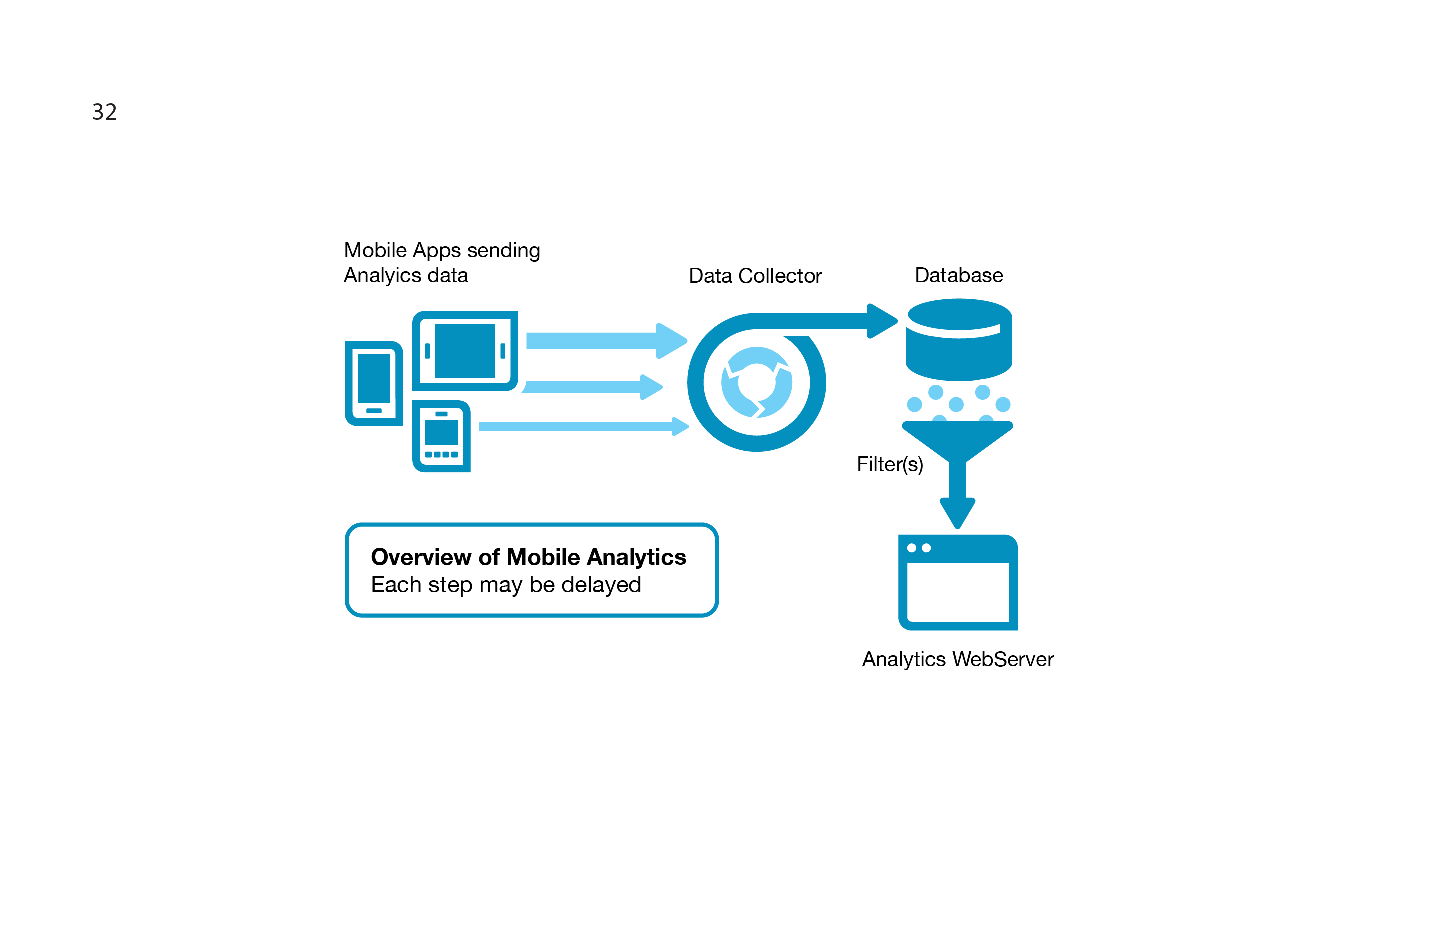
\includegraphics[width=\linewidth]{images/mobile-analytics-playbook/Chart-08-Overview-of-MobileAnalytics.pdf}
    \caption{Overview of Mobile Analytics~\cite{harty_aymer_playbook_2016}}
    \label{fig:map2016-overview-of-mobile-analytics}
\end{figure*}

An overview of Mobile Analytics was published in The Mobile Analytics Playbook,~\sidecite{harty_aymer_playbook_2016}, and the figure is reproduced here with permission in Figure~\ref{fig:map2016-overview-of-mobile-analytics}. The overall approach also applies conceptually in terms of how either apps (often delegated to the analytics library implementation) or the device sends the data. As an observation, the approach would also work if the data is transferred using other conduits, such as copying the data using a memory card, however these details are unlikely to apply to the vast majority apps and even for those developers the conceptual model is unlikely to change materially.

Transmission of the contents of the logs and/or mobile analytics data is asynchronous and may occur almost immediately, or in some rare cases months later. In a discussion on the Android implementation of the popular segment.io library, a non-profit reading app needs to store up to six months of reading analytics on the device using this library. The authors discussed practical ways to store the analytics events without loss and then to be able to upload them correctly even where network connectivity is unreliable~\sidecite{segmentio_supporting_6_months_offline}. Several analytics providers have documented their transmission mechanisms. \emph{``Crashlytics limits logs to 64kB and deletes older log entries when a session's logs go over that limit."} and it~\emph{``...only stores the most recent eight recorded exceptions. If your app throws more than eight exceptions, older exceptions are lost."}.  The non-fatal exceptions are sent the next time the app launches~\sidecite{firebasecrashlytics2020_customize_crash_reports}. In contrast the Segment implementation for Android stores up to 1000 events~\sidecite{segment_analytics_for_android_docs}.

One of the particular implementation details may be worth considering, which is the growth in intermediaries and their adoption by developers. Segment provides one such service, where they provide developers with a single per-client app API that then wraps hundreds of potential implementations and offers two \emph{``connection modes"}, device and cloud~\sidecite{segment_analytics_for_android_docs}. When using their cloud-mode~\emph{``Segment sends messages to the Segment servers, and then translates and forwards that data on to the downstream tools."} Their service becomes a vital additional component in the process and may affect many aspects of the data including privacy, who can analyse it, and latency implications.   

\subsection{Data funnels from users to devs}
The following list itemises a set of possible stages in a data funnel for data that originates from a user's device until it is available for use by the development team. real-world funnels are likely to include a subset of these, in a particular order in terms of the data flow.

\begin{itemize}
    \item Per-app implementation and options
    \item Per-analytics/logging library implementation and options
    \item Farming the log (and/or potentially other usage data) data on device
    \item Device model and operating system combination
    \item Per device implementation and options
    \item Data daemons that control/negotiate what data is and is not available/provided
    \item Data privacy screening (can occur at various points in the funnel)
    \item Batching, queuing, limits, latencies, transmission triggers, ...
    \item Connectivity quality and reliability
    \item Network behaviours e.g. where traffic may be blocked in some geographies, by some network providers, etc.
    \item Data Collector inbound processing (filtering, buffering, validity checks, non-repudiation, dealing with spoofing, fakes, etc.)
    \item Analytics tool filtering and reporting. This may include muting of some aspects of the reporting e.g. for issues considered no longer actionable. 
    \item Content access, storage, combination with other sources, further reporting, etc.
\end{itemize}

Note: there may also be data injected into the funnel, for instance through \href{https://en.wikipedia.org/wiki/Synthetic_monitoring}{synthetic monitoring}, testing of the apps and/or the analytics clients and APIs, spoofing, denials of service, and so on. 

MUST-DO add figure, write up this section.




\section{Conceptual model of usage analytics}
Usage analytics pertains to recording and analysing the usage of software. Application usage analytics is mentioned in various sources, including patents filed by Google in the USA~\emph{e.g.} for methods and systems to collect and provide application usage analytics to developers~\sidecite{googlepatent_hyman2016_collecting_application_usage_analytics}. 

Conceptually there appear to be four broad levels of usage analytics, these are illustrated in Figure \ref{fig:four-layers-of-analytics-for-mobile-apps} and described next. These four levels can be approximately mapped~\sidenote{The approximation is because software is not quite so cleanly cut into layers or levels. For instance app-level mobile analytics can be used to record many aspects of GUI activities, albeit unnaturally. Also, the operating system can observe aspects of the GUI, for instance by instrumenting the Accessibility APIs, a topic I touch on in one of the appendices.} to the three layers of an app:

%\akb{Are 'Visual' analytics tools automatically 'Mobile' tools as well? The \textit{heatmapping} example seems to be one that could fit into both layers}

Their use will be discussed in more detail in the chapter titled~\href{chapter-applying-analytics-to-development-practices}{\emph{\nameref{chapter-applying-analytics-to-development-practices}}}. %MUST-DO decide whether layer and level are synonymous, and if not whether to use one term or the other. Anyway I'm aware I may be conflating both terms here and want to improve the precision of whichever term(s) I use. 

\begin{figure*}
    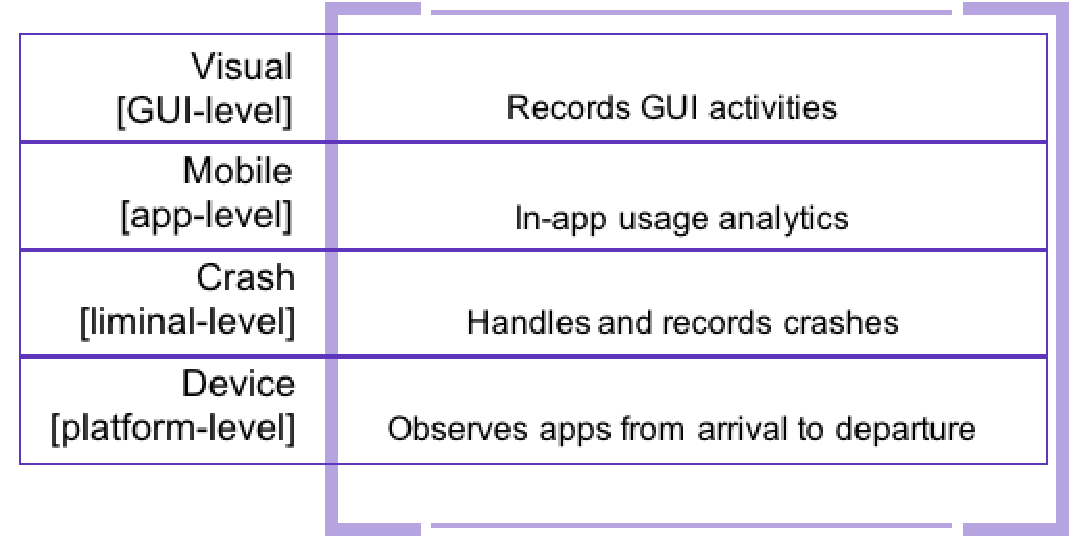
\includegraphics[width=\linewidth]{images/4-layers-of-analytics.pdf}
    \caption{Four Layers of Analytics for Mobile Apps}
    \label{fig:four-layers-of-analytics-for-mobile-apps}
\end{figure*}

\begin{itemize}
    \item \textbf{Visual (GUI-level)} operates at the GUI level, or layer, of the app. It records aspects of the GUI activities such as touches, gestures, interactions with the screen, and data entry. Often it includes recording what is on the screen too. A common type of Visual analytics is \emph{heatmapping} software. Note: visual analytics may be \emph{implemented} in the app, conceptually they observe the GUI as if from above the UI.
    \item \textbf{Mobile (app-level)} is incorporated as part of the app and records aspects of what the app is doing, in effect aspects of the usage of the app. Mobile Analytics is prevalent in Android apps and already used for various business purposes.
    \item \textbf{Crash (liminal-level)} is where specialised reporting can intercept crashes. Through the interception they can change the behaviour of the app, for instance to provide a better user-experience, log, and report the crash to the developers. \emph{Fatal crashes} are ones where the application quits. These can also be observed by the operating system; for mobile apps the operating system is an intrinsic part of the platform.
    \item \textbf{Device (platform-level)} Platform-level analytics can record apps from when they are installed until they are removed. This recording can include details such as when apps are in-use, crashes, freezes, and so on. Both of the dominant platforms (iOS and Google Android) allow users to decide whether their devices will share this data.
\end{itemize}

% https://new-wine.org/resources/blog/living-liminality-lessons-trust-gratitude-prayer-compassion-global-church-dd508239ff5

This research includes case studies and developer reports of examples of analytic tools that cover three of these four layers of analytics. The remaining layer, visual analytics, is described briefly with a few examples, visual analytics is seldom used in production mobile apps and therefore it was excluded these from the core research. They may be an interesting topic for future research particularly given some of the potential benefits of visual analytics. % COULD_DO add notes on privacy issues and other complicating factors in this sort of research. 


\section{Conceptual model for DevOps}
DevOps recognises the benefits of connecting development and operations of software. a Yin Yang symbol recognises there's some negative in the positive and vice-versa. Conceptually, teams can choose to invest in operations while they're developing to improve the operational aspects of their software, for instance by designing in good operability. Similarly when the software is in use by observing the software's behaviours operations can improve the development. Examples include: considering the how improvements could be developed or the software development lifecycle process improved based on how the software is being used.

\begin{figure}
    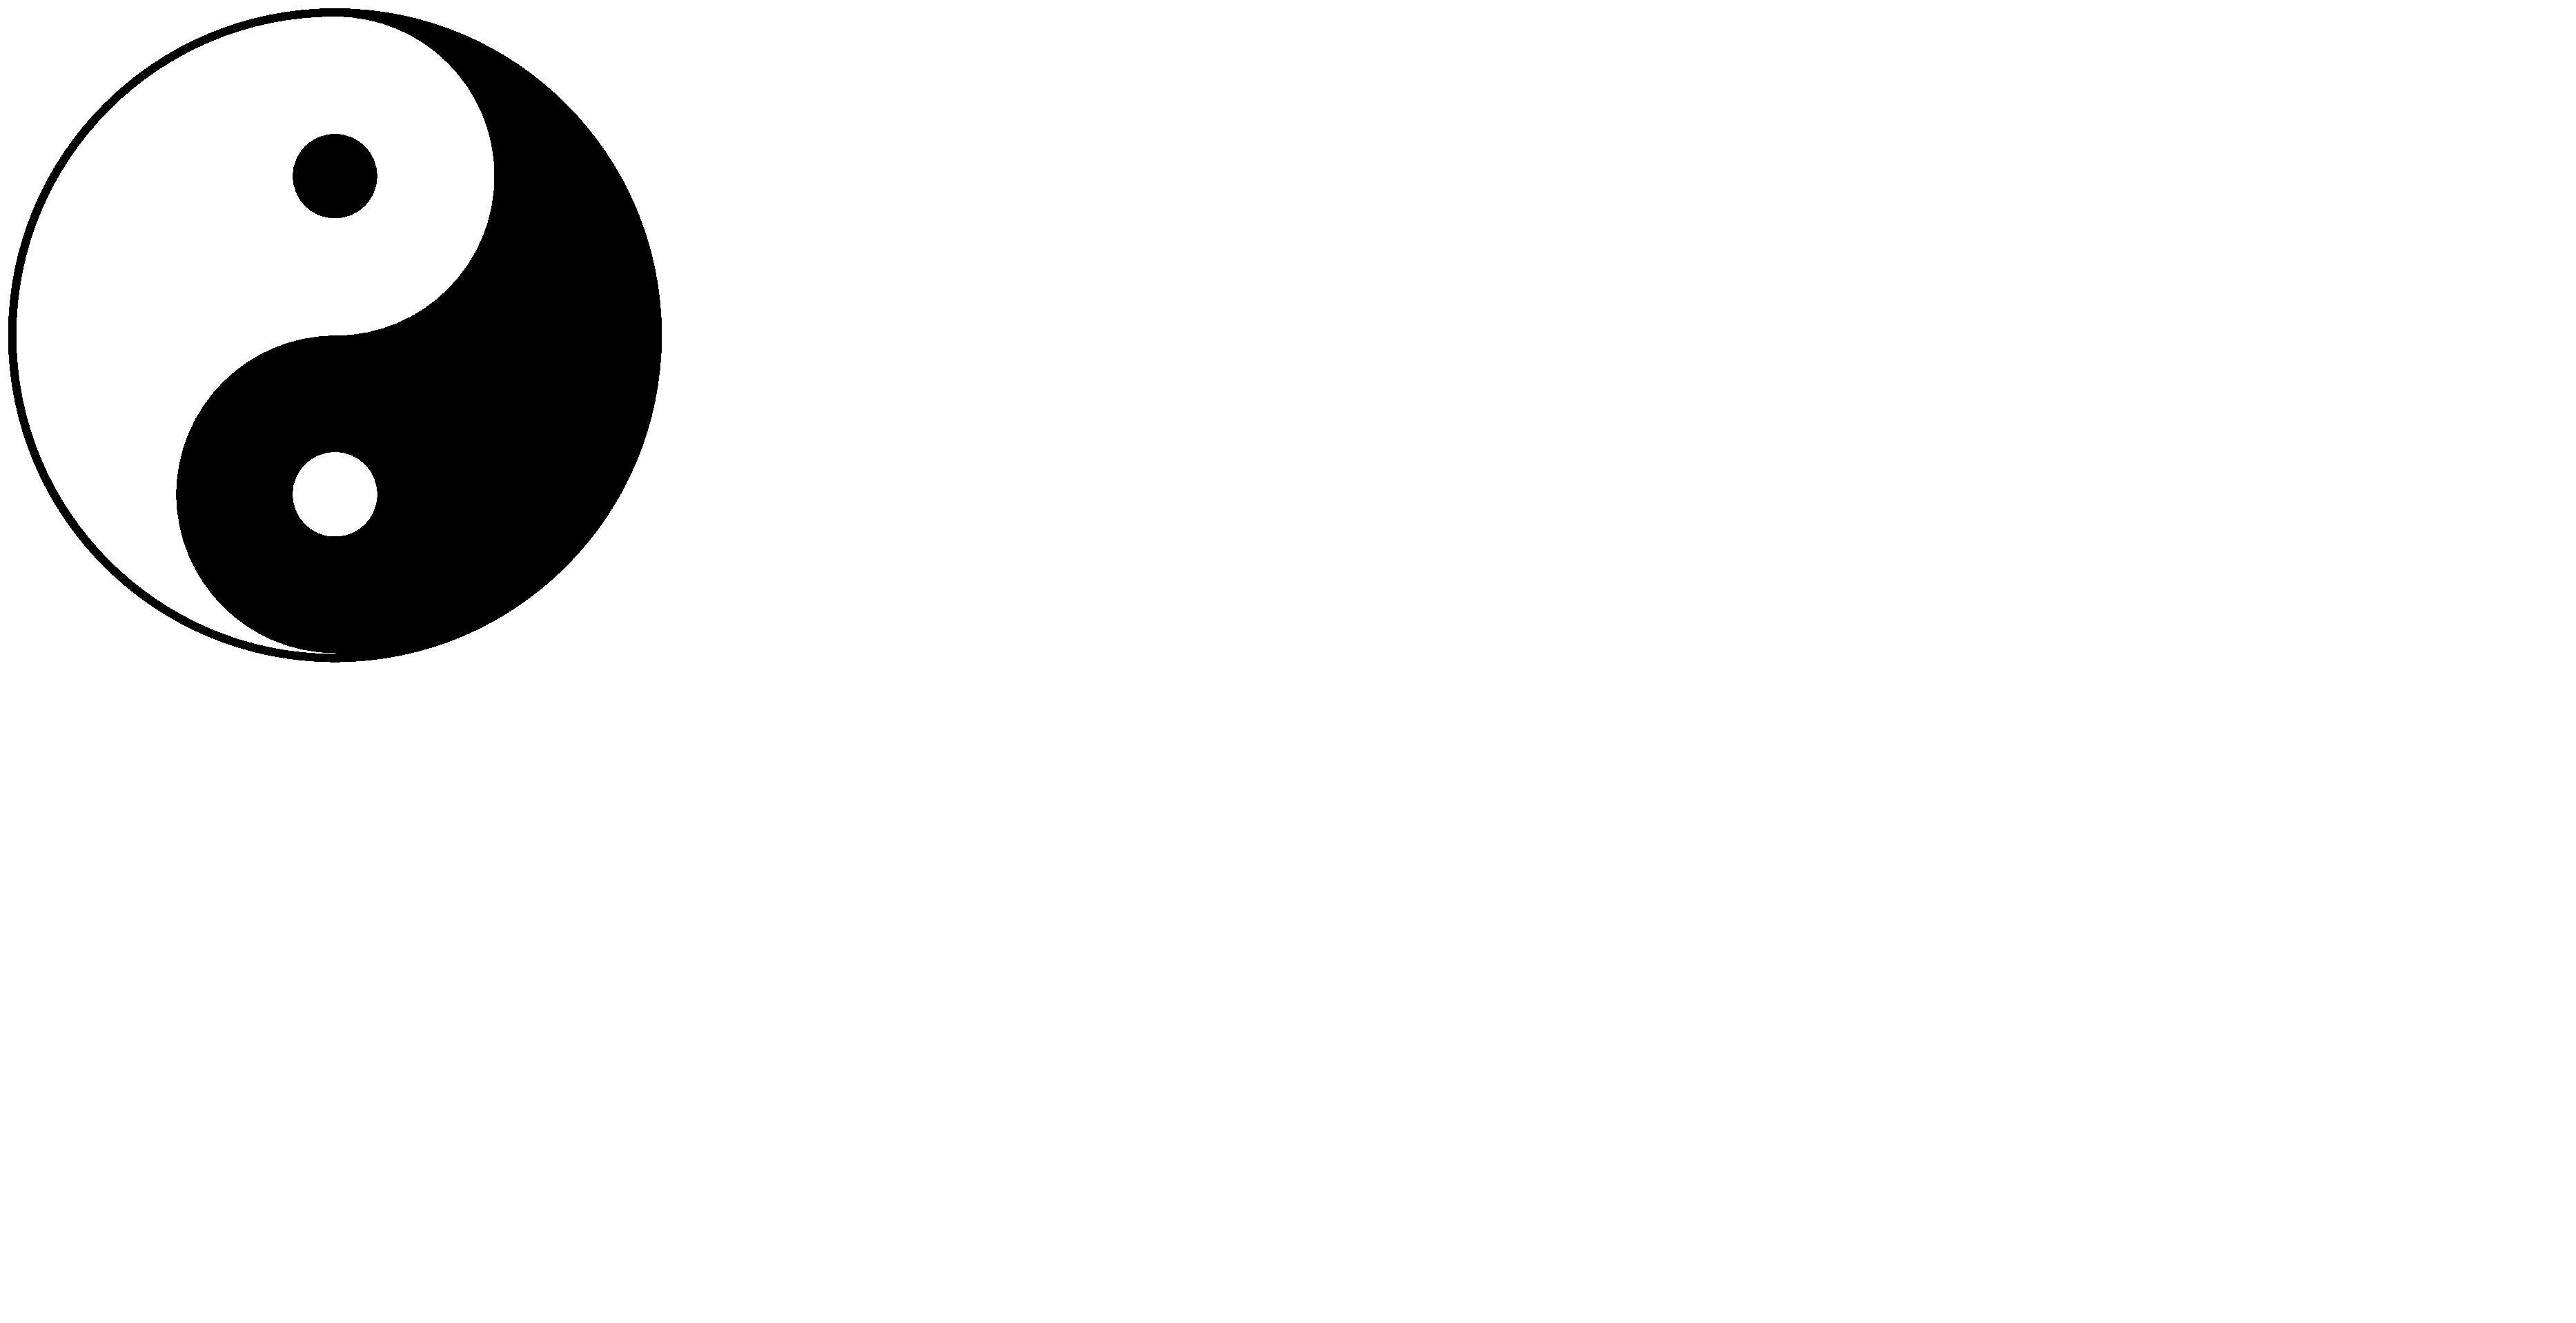
\includegraphics[width=0.5\linewidth]{images/wikipedia/Yin_yang.pdf}
    \caption{Yin Yang to represent DevOps}
    \label{fig:yinyang_for_devops}
\end{figure}



One of the popular concepts in DevOps is represented by an infinite loop in the shape of a horizontal figure of eight like diagram, illustrated in Figure~\ref{fig:atlassian-state-of-devops-report-2016-devopsloop}.~\sidenote{This example is from a blog post by Atlassian~\url{https://www.atlassian.com/blog/devops/2016-state-of-devops-report} announcing \emph{``The State of DevOps report"} 2016 edition.} There are many variations of this illustration available, perhaps unsurprisingly given the popularity of DevOps and those who write and publish on the topic who may want to give their own spin on the topic.

\begin{figure*}
    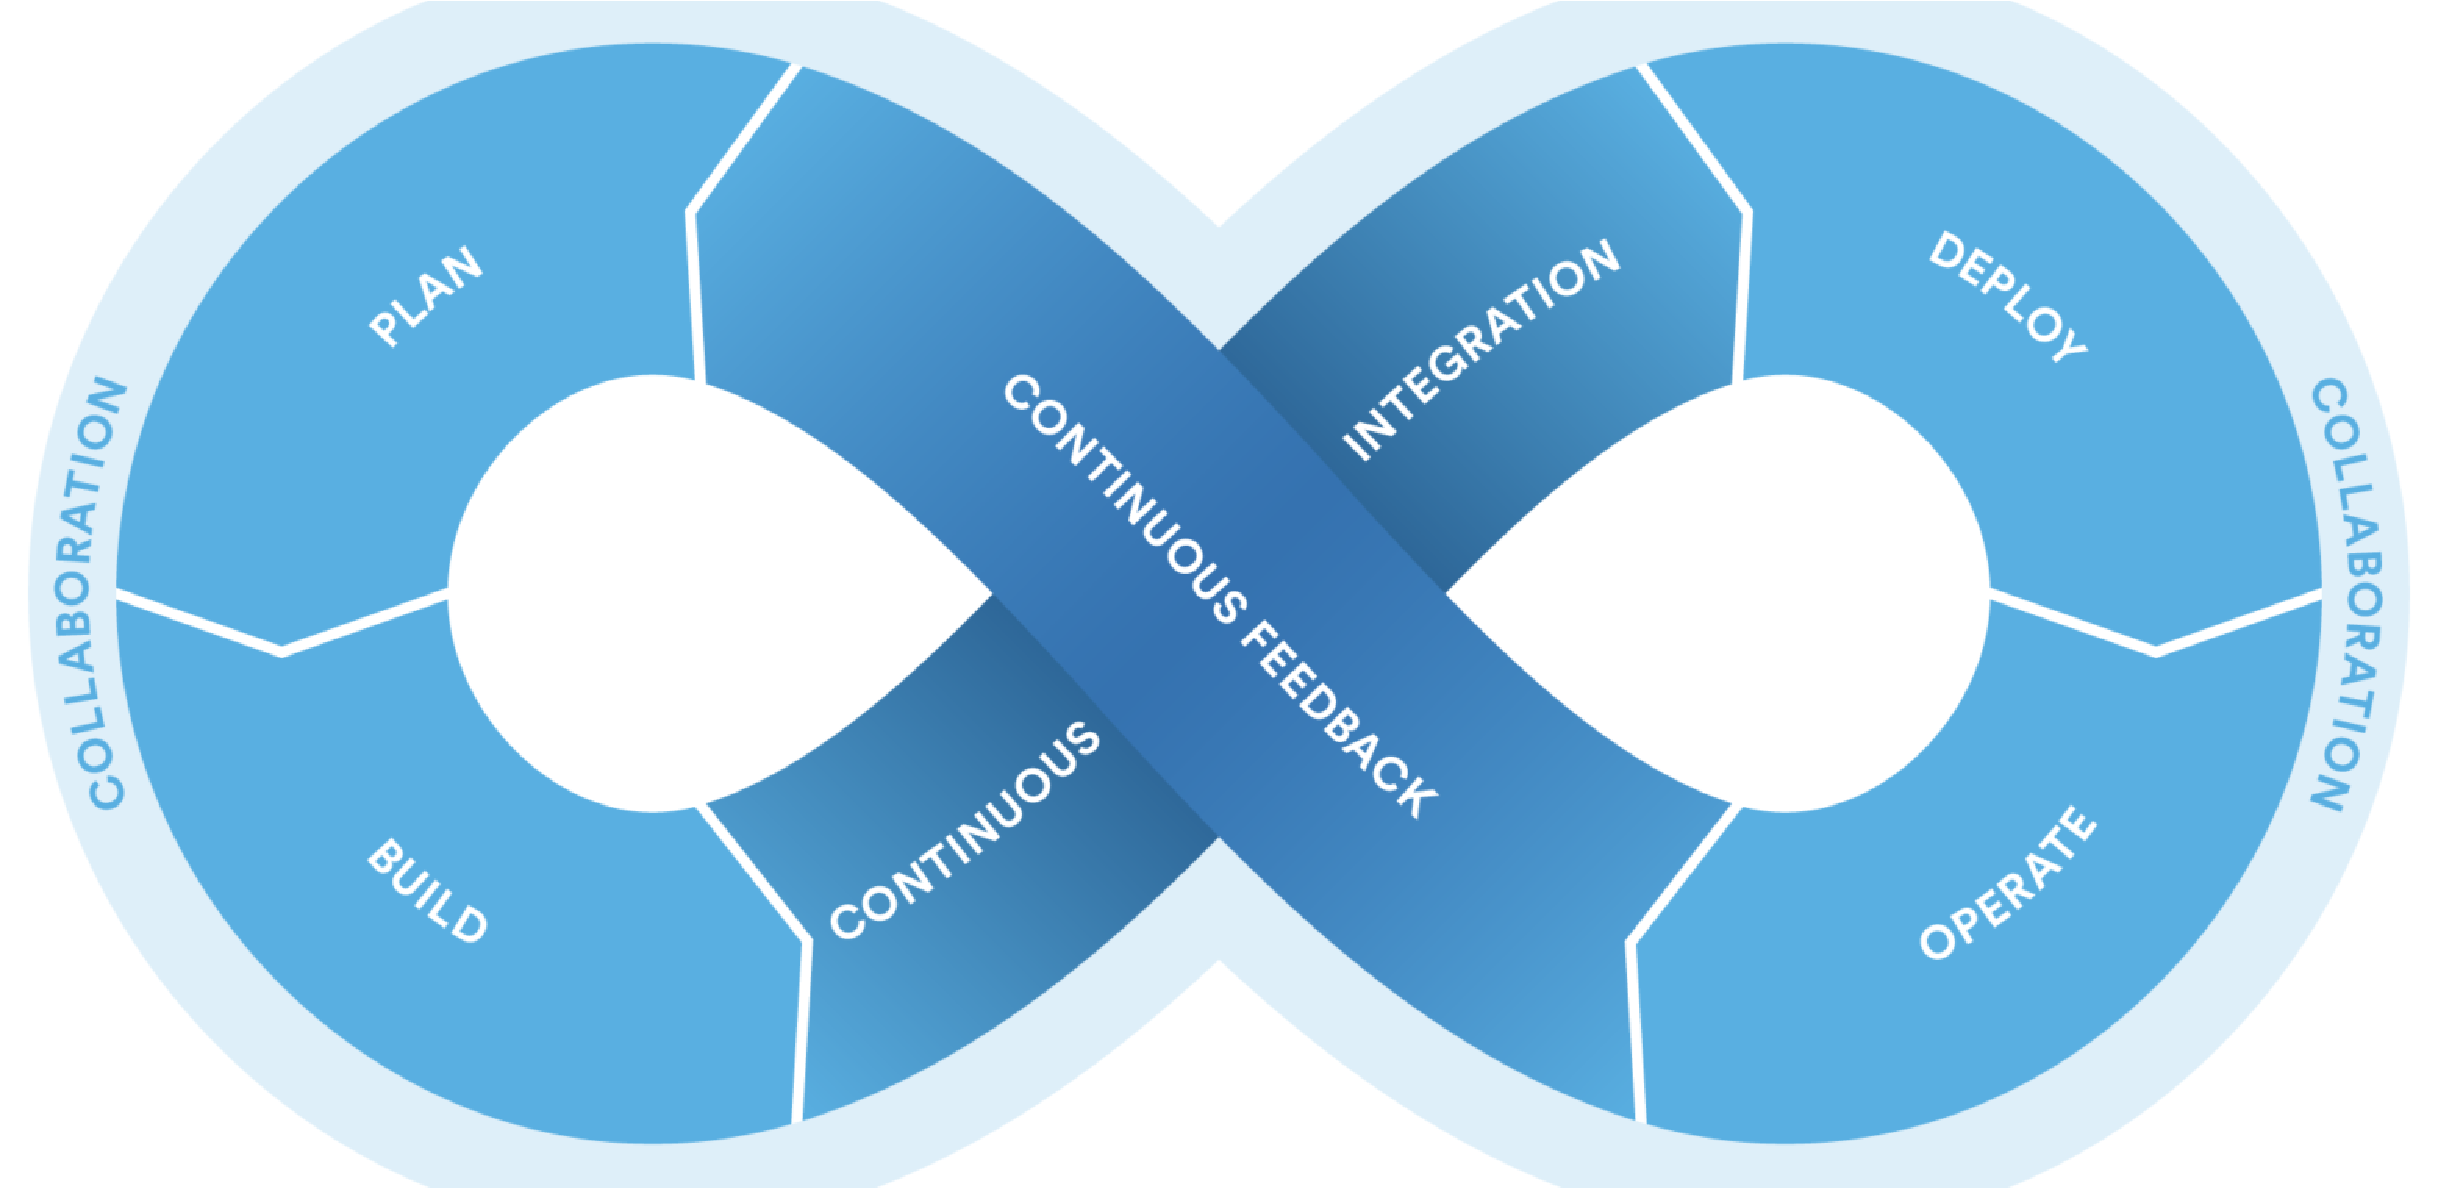
\includegraphics[width=\linewidth]{images/atlassian/atlassian-state-of-devops-report-2016-devopsloop.pdf}
    \caption{Atlassian DevOps loop}
    \label{fig:atlassian-state-of-devops-report-2016-devopsloop}
\end{figure*}
% https://3kllhk1ibq34qk6sp3bhtox1-wpengine.netdna-ssl.com/wp-content/uploads/devopsloop-1560x760.png



\section{From conceptual models to practicalities}
The previous sections introduced five conceptual models that help to establish the context for the ecosystem, structural aspects of mobile apps and perspectives where mobile apps can be observed, analogue and digital feedback, usage analytics and DevOps considerations. The next five sections cover various practical aspects of mobile apps including development and usage lifecycles, information sources and finally choices for engaging with analytics.


\section{Mobile apps and development team's mobile devices}
A mobile app is more than compiled source code, it includes various resources such as text, images, audio, screen layouts, and sometimes other contents. Many include software libraries from one or more sources. Mobile apps are also digitally signed. Data and information can be obtained for these various constituent parts, for instance some failures may occur within a library at run-time and be reported in logs and via mobile analytics.

Development team's mobile devices, with occasional exceptions are often the same device models that end users have and use; and furthermore they have similar end-user accounts and the majority of their apps are installed in similar ways to those installed on end-user devices. These similarities have some important implications - data on the usage of these devices by the development team may also be collected and considered as being part of the end-user population, and any in-app analytics in the various installed apps may provide their data to the respective mobile analytics systems,~\emph{etc.}

These devices may be configured differently and they may also run local builds and internal releases of apps. The apps may be configured to provide different amounts of information in local logs and/or using mobile analytics libraries for instance to either distinguish the usage or to suppress data from being shared. Knowing and understanding these nuances can help interpret some of the sources of data and information pertaining to these devices and apps.


\section{Mobile app development lifecycle}
To provide some context for this section, Figure \ref{fig:ci-cd-development-and-feedback}~\sidenote{Reproduced from \emph{``An empirical study of architecting for continuous delivery and deployment"}~\cite{shahin2019empirical_study_architecting_cd}}
illustrates a modern continuous software lifecycle including feedback. We can observe several distinct stages in the development and deployment of software and the feedback each stage can provide. %MUST-DO check the guidelines for reproducing and citing a figure as-is.
%
In contrast, Figure \ref{fig:google-play-app-development-and-feedback} illustrates a similar software lifecycle for Android apps released through Google Play together with the various forms of feedback~\sidenote{Here we have excluded feedback from the app store, nonetheless it exists for many app stores.} 

Key differences between typical CI/CD lifecycles and the one for Google Play is the pre-launch testing and the app store providing both user feedback and a service called Android Vitals. The pre-launch reports are generated automatically by Google where the app store runs automated monkey testing on a farm of Android devices and various static analysis checks of releases deployed to any of the test channels. They are described in~\href{subsection-test-channels}{Test Channels}. %MUST-DO actually add information on the test channels and how releases can be promoted to production releases in Google Play.


\begin{figure*}
    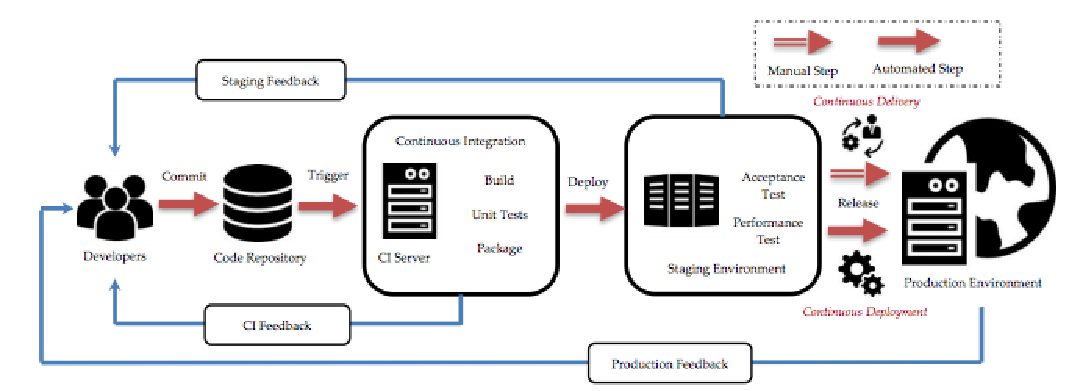
\includegraphics[width=\linewidth]{images/ci-cd-development-and-feedback.pdf}
    \caption{CI/CD development and feedback, reproduced from~\cite{shahin2019empirical_study_architecting_cd}}
    \label{fig:ci-cd-development-and-feedback}
\end{figure*}

There are additional sources of \emph{analogue feedback} from people, including from alpha and beta testers and end users; and \emph{digital feedback} from Google tools and from usage data collected from the field. These terms are expanded in the section~\href{analogue-and-digital-feedback}{\emph{\nameref{analogue-and-digital-feedback}}}.

% Vel This figure doesn't appear in the generated PDF file. I don't think I've used minipages (at least not earlier in this chapter) David Carlisle proposes https://tex.stackexchange.com/a/85153/88466 to help find the missing float, however I still don't understand the cause of the missing float.
\begin{figure*}
    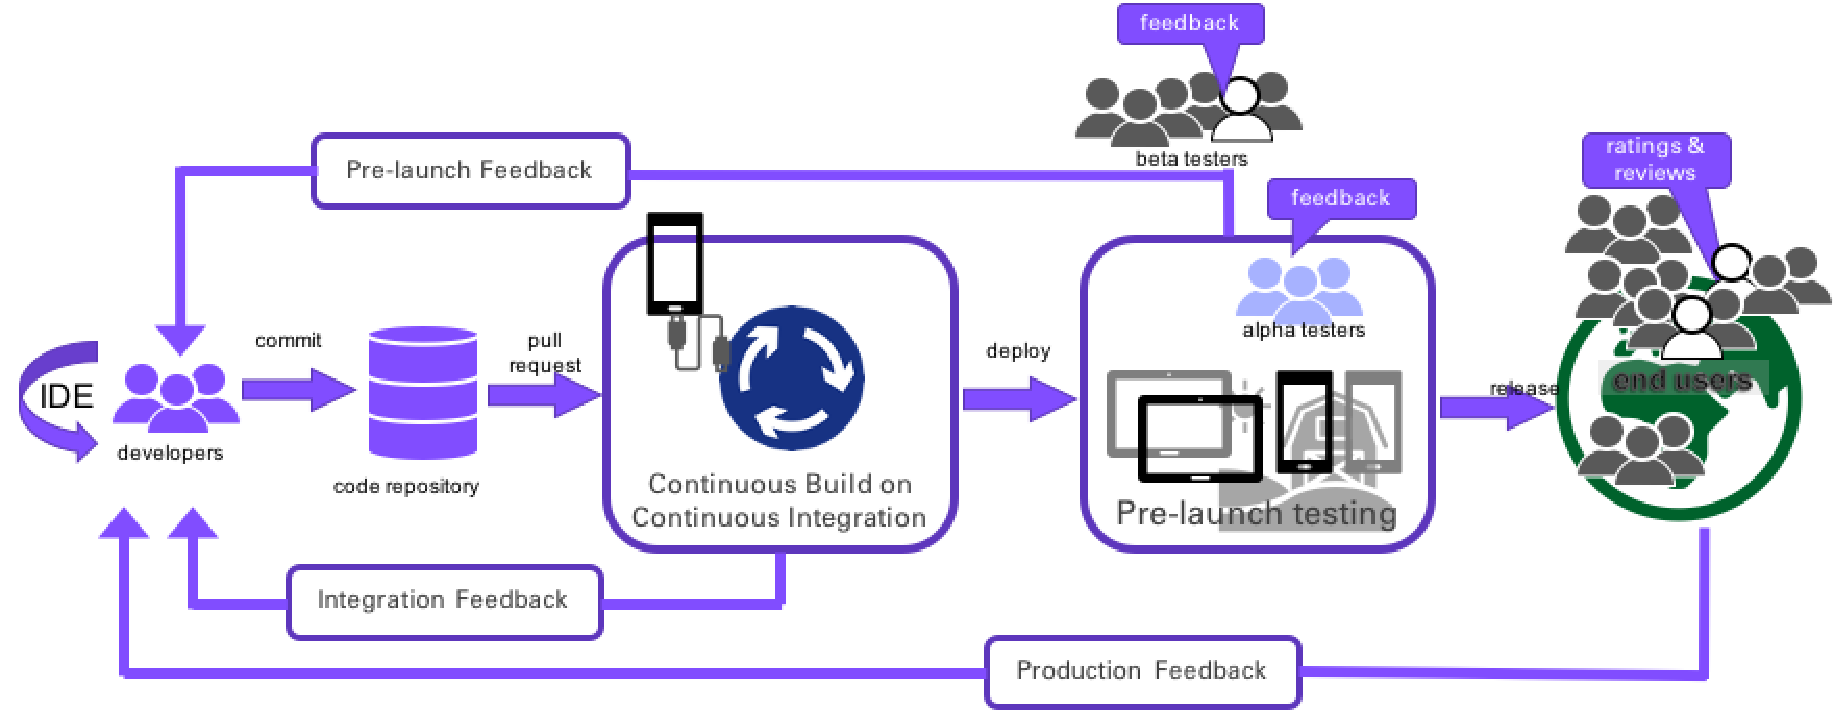
\includegraphics[width=\linewidth]{images/google-play-app-development.pdf}
    \caption{Google Play App Development and Feedback}
    \label{fig:google-play-app-development-and-feedback}
\end{figure*}


\section{Mobile app usage lifecycle}
Mobile apps have a usage lifecycle, which starts when an app is chosen to be installed and ends with either abandonment or active removal of the app from a device. Figure~\ref{fig:mobile_app_usage_lifecycle}~\sidenote{Based on a figure in~\cite{bohmer2011falling_asleep_with_angry_birds}} illustrates the possible stages of a mobile app's life on a user's device. Google Play Console collects data consistent with this lifecycle, analyses it and provides aggregate reports based on their analysis. 

For clarity and completeness there is another lifecycle when the app is running, described in the Android documentation as the \emph{``Processes and Application Lifecycle"}~\sidecite{android_processes_and_application_lifecycle} These are more detailed and are not included in the reports Google provides developers. %(I doubt their details would be recorded either). 
Note: the processes and application lifecycle may affect how in-app analytics libraries behave, including when they transmit their data to their respective central servers.

% More info and code samples: https://www.vogella.com/tutorials/AndroidLifeCycle/article.html

\begin{figure*}
    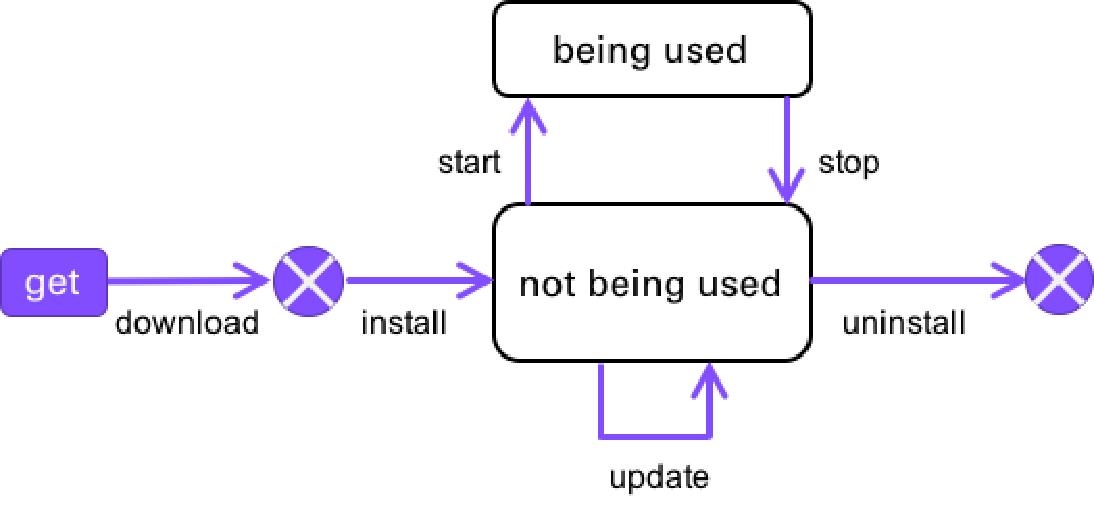
\includegraphics[width=\linewidth]{images/mobile_app_usage_lifecycle.pdf}
    \caption{Mobile App Usage Lifecycle}
    \label{fig:mobile_app_usage_lifecycle}
\end{figure*}

A later section~\href{sec:platform-level-analytics}{\emph{\nameref{sec:platform-level-analytics}}} provides a proposal of how Google collects the underlying data (they do not document, explain or encourage research in how their system works, We return to their (Google's) reported behaviour and the effects later in this thesis). % MUST-DO add link to: Developers banned from app store ecosystem and their apps removed.
And the chapter \href{app:software-contributions}{\emph{\nameref{app:software-contributions}}} describes software we developed to help collect data from Google Play Console in order to facilitate both research and to enable developers to collect and use data...

Crashes are often considered a concrete measure of poor performance of software and there has been extensive research in crashes for Android applications, in particular. I suspect there are various reasons for the focus on crashes as an oracle for testing software, crashes are unambiguous (even if the causes are not) and they are also binary so easy to determine whether software has, or has not, crashed. 

In 2017, Google launched a service called Android Vitals as a new, intrinsic part of Google Play Console,~\sidecite{googblogs_I_O_2017_everything_new_in_the_google_play_console}, where they popularised a measure called \emph{Stability} to assess the quality of Android apps. Their measure includes both crashes and when an application freezes or is unresponsive for at least 5 seconds from a user's perspective, a term Google call Application Not Responding (ANR).


\subsection{DevOps for mobile apps}
This section starts with an overview of DevOps concept of an infinite loop for software generally before becoming more specialised on DevOps for mobile apps. %SHOULD-DO consider expanding this section. TBD how much I should write about the concepts and terms. 
The focus here is on data from various stages of a conceptual infinite combined development and operations process to indicate where mobile analytics applies in terms of providing data to the development team. This data includes: log data, static analysis results, test results, release and usage data, and mobile analytics data and reports.

In October 2020, one of the students taking part in the PhD symposium at the ICST2020 conference presented a variation of the DevOps loop (as illustrated earlier in this chapter in Figure~\ref{fig:atlassian-state-of-devops-report-2016-devopsloop}) that is relevant to this research. In the student's figure their focus was on crash reproduction and this illustration is temporarily illustrated in Figure~\ref{fig:crash-reproduction-icst2020}(~\emph{pending an update from the presenter of that topic}).

\begin{figure*}
    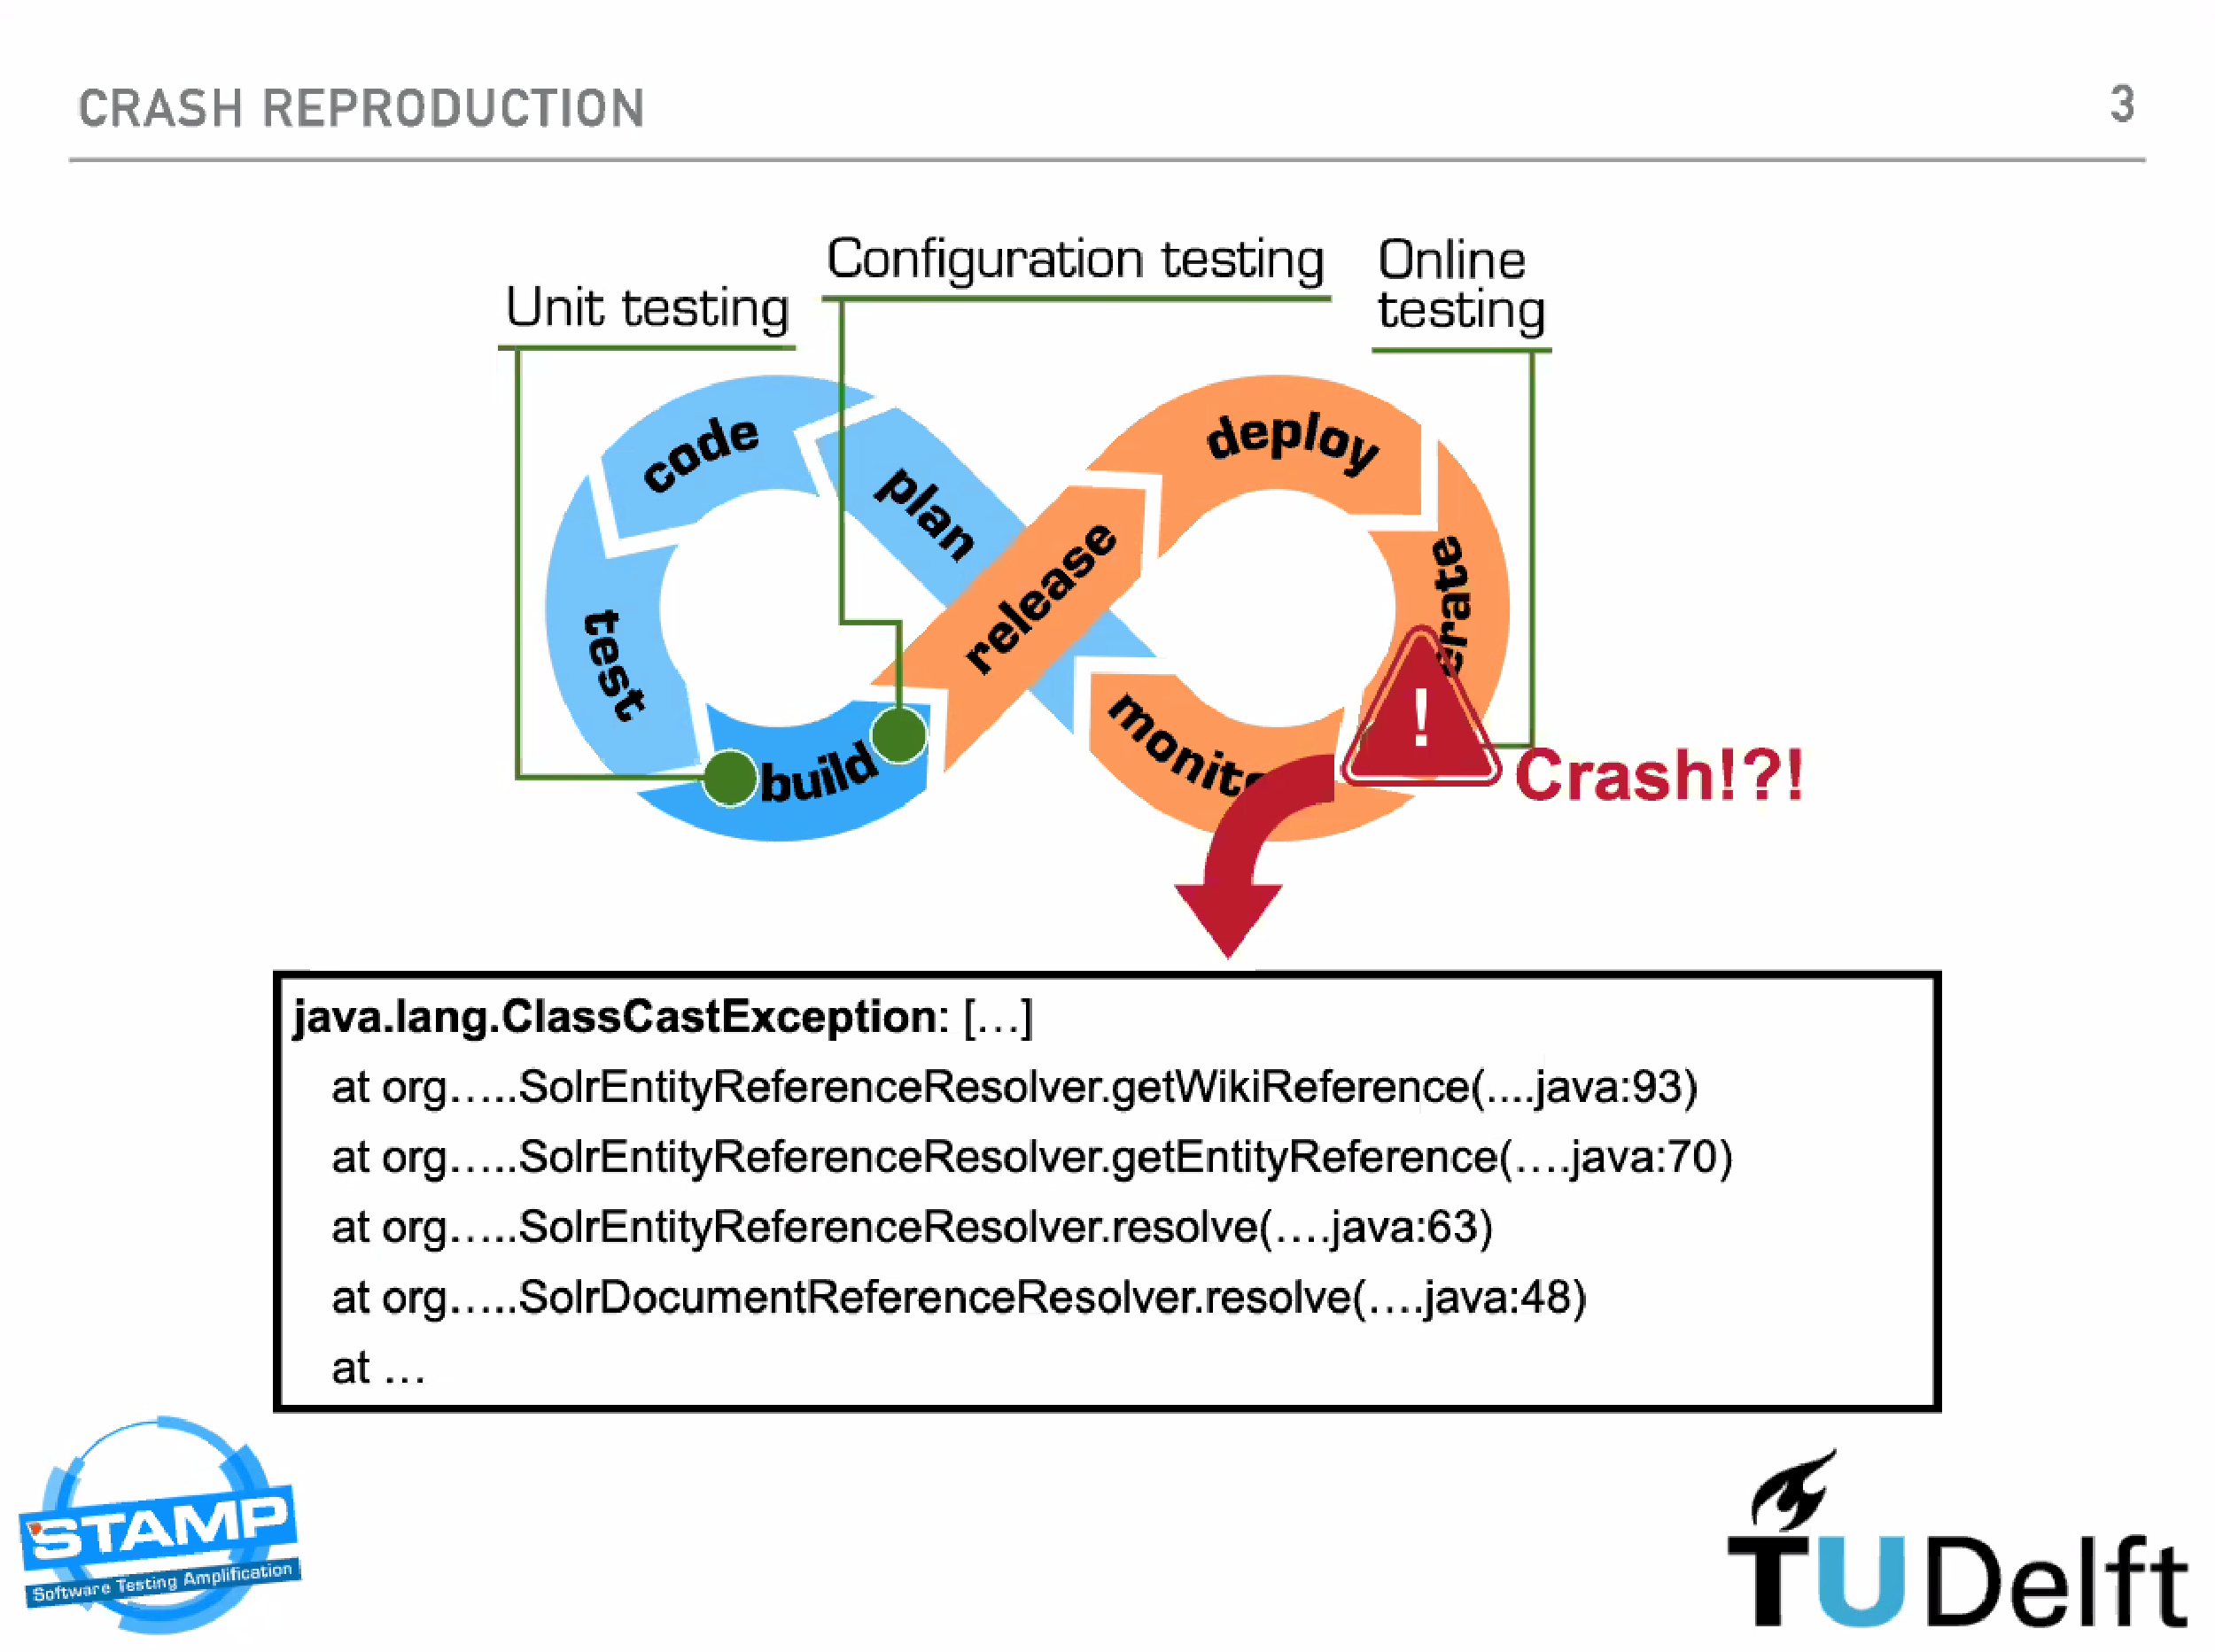
\includegraphics[width=\linewidth]{images/icst-2020/crash-reproduction-icst2020.pdf}
    \caption{Temporary image: Crash Reproduction}
    \label{fig:crash-reproduction-icst2020}
\end{figure*}

Figure~\ref{fig:oberve-and-apply-devops-loop} is revised illustration that shows, in red, the extent software can be observed, and in green of when the results of those observations can be applied to the code. Note: the observations can be applied throughout every phase, for instance during deployment aberrant behaviour observed during the deployment may lead to the deployment being paused.

\begin{figure*}
    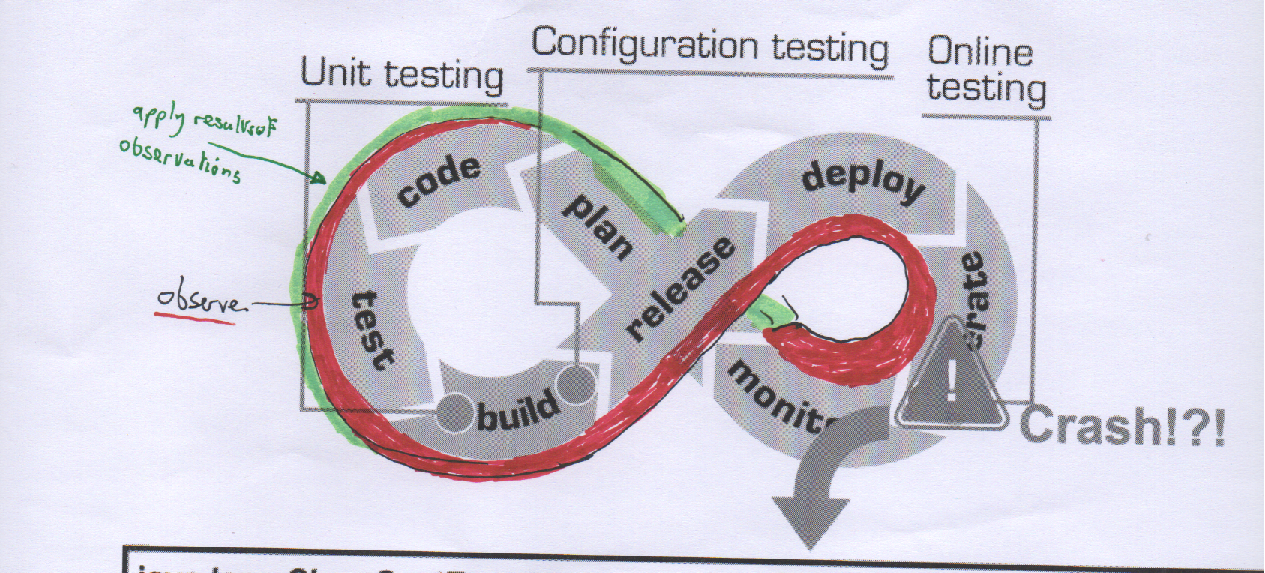
\includegraphics[width=\linewidth]{images/rough-sketches/hack-of-devops-crash-figure.pdf}
    \caption{Rough Sketch: Concept of feedback on software and applying it}
    \label{fig:oberve-and-apply-devops-loop}
\end{figure*}

Data is available using various sources about software from the outset of coding until the software dies; however for the purposes of this thesis the focus is on when the software is actively used and maintained, as illustrated in the previous three figures:~\ref{fig:atlassian-state-of-devops-report-2016-devopsloop},~\ref{fig:crash-reproduction-icst2020},~\ref{fig:oberve-and-apply-devops-loop}. 

During coding code analysis tools such as static analysis identifies patterns of potential concern in the source code and similar artifacts such as GUI layouts, strings in resource files, and so so. Tests can also be created and performed from the outset of the coding to provide runtime feedback (~\emph{i.e.} data) about the software under test, and similarly developers can add logging statements and also use logging built into the operating system that both provide data that can be mined to learn about the software's behaviours.

The build process may include configuration details, for instance to create a range of custom applications, to include instrumentation, to compress and obfuscate the application binary, and to create debug and release editions of the software. Data about the build process and about what has been built may also be observed and analysed and the products tested and analysed; for example an application binary can be scanned for information leakage in an obfuscated build, and builds can be tested to provide more data about how the software performs.

The release and deployment phases will be covered in more detail in the next section; here the focus is on the data available as part of these phases. 

As software is released the software transitions from being within the view of the development team to being used by others where the development team no longer has direct access to the devices that have the app installed or being used. They are remote from the use of the app. This means that local access to devices (to see what's happening and to try things out) and to the device's logs are unlikely to be practical, other sources of information now need to take precedence.

The release of a mobile app using an app store is subject to the processes and controls applied by the provider of the app store. The app store may offer both free and paid-for optional services to the developer, for example Google provides optional, free pre-launch reports that contain the results of automated testing and static analysis of application binaries. The app store may provide reports to the development team particularly if they decide to delay or block a release or suspend an app from being downloaded by end-users.

Usage is the ultimate active phase for a mobile app installed on a user's device. Simplifying slightly, as some apps run automatically in the background, most apps are started and used by end-users. Aspects of the usage can be recorded by various software utilities, in particular by the platform which records when an app starts and when it terminates. The platform can also record when an app is installed, when it is updated, and when it is uninstalled. The app store may provide developers with reports and statistics on the app's install base and usage. The app store may also provide developers with information about the performance of the app including any failures of the app while it was running.

Crashes are logged locally by the platform, some platforms may also record other failures and performance related data as well as resource utilisation and various capacities such as battery level locally. The platform may have permission from end-users to forward a copy of the information logged locally on the device and to use it for various purposes.  

\subsection{Software releases for mobile apps}
For mobile apps, the release management may include deployment of the app to end-user's devices either as a fresh install for new users or as an update for existing users that app on a given device~\sidenote{Mobile apps for Apple and Google app stores are installed per device and licensed per user so users can freely choose how many devices to install an app on, and they may even have different releases of the same app on different devices.}.

Releases may be acute or chronic in nature. Acute releases are actioned immediately and deployed as soon as practical. Chronic releases may involve alpha (closed-group membership) and beta (open-group membership) testing followed by rollout in stages, for instance starting at 10\% of the user-base, then increasing to 25\%, and so on until the new release is available to 100\% of the user-base. Note: there is no guarantee that the new release will be deployed to the entire user-base, and in my experience some users will keep using much older releases for as long as several years after newer releases were made available to them. 

The actual deployment and market penetration of a new release depends on several factors which may be outside the developer's direct control. This particularly applies for mobile apps made available through an app store where the app store and end-users can block new releases being applied. In my experience across a range of Android apps, for a 100\% rollouts it takes about a week for the new release to be installed on 50\% of the user-base's devices, however the range varies from 3 days to several weeks to reach 50\%.  

\begin{figure*}
    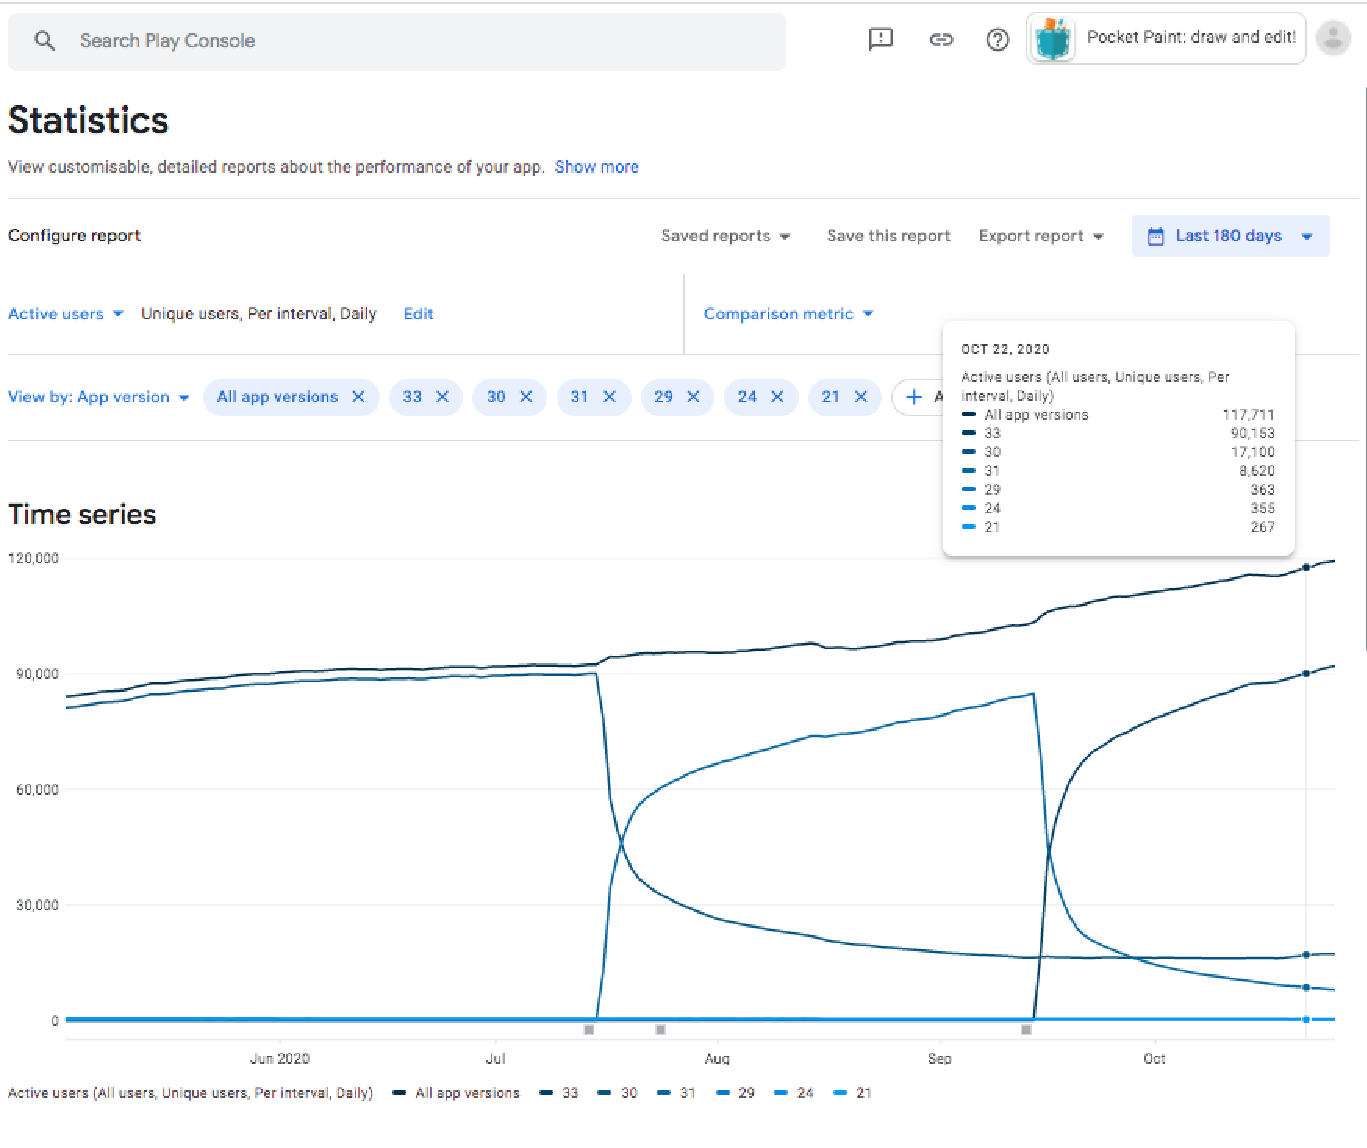
\includegraphics[width=\linewidth]{images/android-vitals-screenshots/catrobat/PocketPaint-ActiveUsers-180days-2020-10-29.pdf}
    \caption{PocketPaint Active Users 180 days by app version}
    \label{fig:pocketpaint-180d-active-users}
\end{figure*}

Figure~\ref{fig:pocketpaint-180d-active-users} illustrates a typical pattern of the majority of the userbase migrating from one app release to another and yet others remain with older releases during this period of 180 days (apologies for the small text in the image it was impractical to resize it adequately). Note: Google defines active users as:~\emph{``
The number of users who have your app installed on at least 1 device that has been turned on in the last 30 days"}~\sidenote{Text extracted from the online help for the `Active users' contextual help icon in Figure~\ref{fig:pocketpaint-180d-active-users}.} so it's not necessarily those who use the app in this period. The residues of users who remain on older releases of the app constrains the rate of change of the overall statistics as measured by Google Play Console and Android Vitals. This means that old buggy releases may continue to adversely affect the overall stability metrics for the app for long periods, even for months and years. Conversely, the project team may have addressed some of the causes of poor stability yet don't have a viable way of proposing users upgrade to the newer releases, and sometimes newer releases may have undesirable features or characteristics from an end user's perspective.

\begin{figure*}
    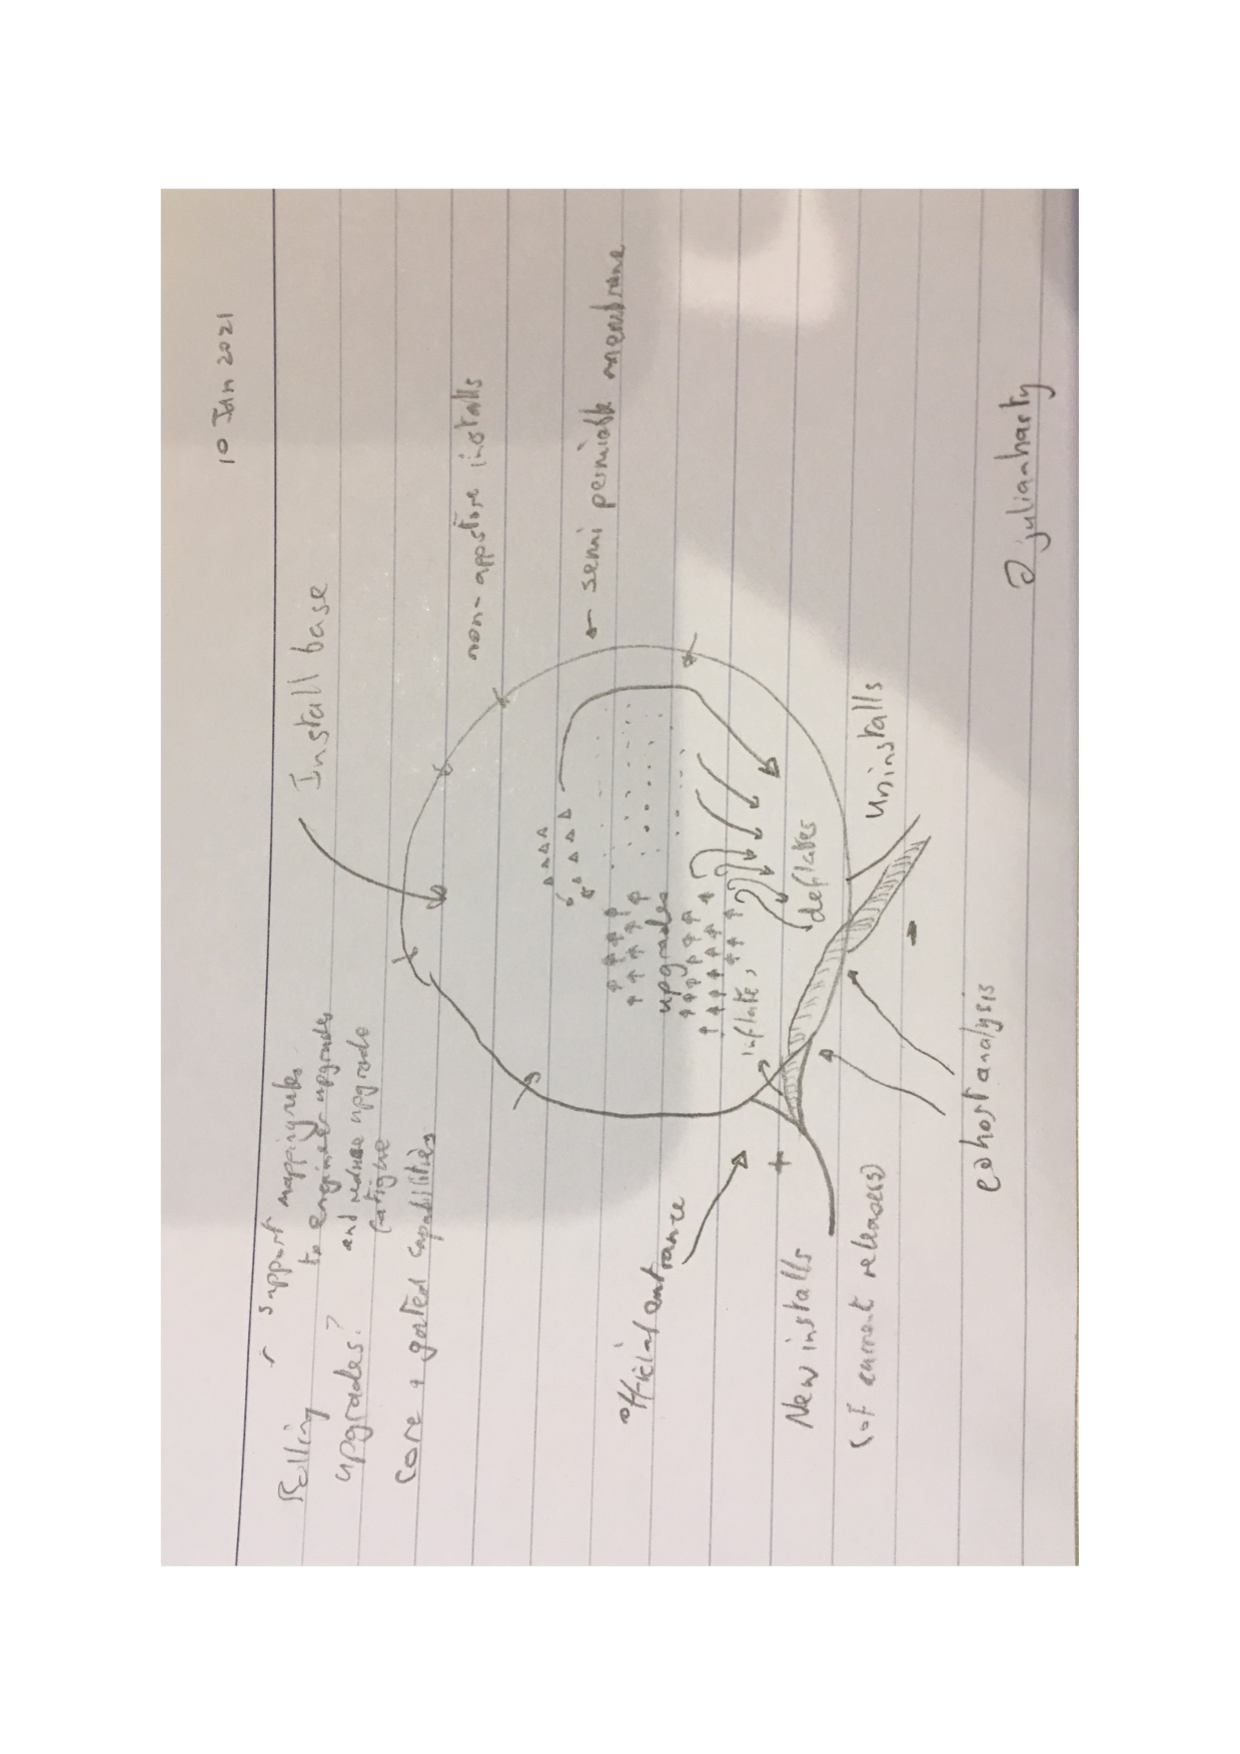
\includegraphics[width=\linewidth]{images/rough-sketches/app-install-base.pdf}
    \caption{App install base}
    \label{fig:app-install-base-rough}
\end{figure*}

\textbf{Installation base}: The rough sketch in Figure~\ref{fig:app-install-base-rough} illustrates static and dynamic aspects of the installation base for a mobile app. The approximate circle contains the installation base for an app. The size ebbs and flows based on new installs - which inflate the shape, and uninstalls - which deflate it~\sidenote{Note: apps may be downloaded independently of devices, for instance using a web browser~\cite{norwied2012_download_android_install_files}, and they may be installed independently of an app store. Both these traits may affect the accuracy of the installation counts.}. 

In current mainstream app stores users do not get a choice of which release of an app they will receive when they receive it, that choice is made by the app store using one or more releases provided by the developer. The app store may allow developers to choose various criteria for current releases, such as a percentage rollout, and then apply that on behalf of the developer. The boundary may be considered semi-permeable as some installations are not sourced from the app store. A key consideration is that upgrades apply to the install base so they occur within a population and do not change the number of installs. That said they may lead to decreases in the installation base for various reasons. Some users may uninstall an app prompted by learning of a new update of the app - for instance if it requires permissions the user considers intrusive or unsafe; others may uninstall the app after the update, for instance if they believe it is too buggy to merit using. Note: they are not able to revert to an earlier release within the current major app store's practices / constraints. 

To sum up so far, new installs receive the most current release gated by the rollout algorithms implemented by and in the app store. Upgrades also receive the most current release gated by the same rollout algorithms.

\textbf{Cohorts}: represent a group of users who share something in common and measures at intervals through time. Examples include new users who install the app on a particular day or in a particular week. They are used in analysis, for instance to measure what proportion of new users still have the app installed a week later. Cohorts can also be used to group users with a distinct release of an app, and so on. Useful introductions to cohort analysis using Google Analytics are available online~\sidecite{codehouse2020_cohort_analysis, googleanalytics2021_the_cohort_analysis_report}, and cohorts are used in various analytics tools including Google Analytics and Firebase Analytics. 

% https://www.codehousegroup.com/insight-and-inspiration/digital-strategy/cohort-analysis-and-how-to-use-it-in-google-analytics
% CHEST journal: Cohort Studies https://doi.org/10.1016/j.chest.2020.03.014

One reason why users uninstall an app is because of poor quality behaviours by the app. In a survey by Dimensional Research, 3011 participants completed an electronic survey to identify key factors that led to end user satisfaction with mobile apps. The research also `... sought to determine what users did when they were unsatisfied with a mobile app.' (page 5). 
53\% of respondents have uninstalled or removed mobile apps that regularly crashed, stopped responding or had errors and 37\% stopped using the app (page 16)~\sidecite{dimensionalresearch2015_mobile_app_use_and_abandonment}~\sidenote{The report is free of charge upon request: \url{https://techbeacon.com/resources/survey-mobile-app-users-report-failing-meet-user-expectations}}.

To sum up again, the installation base relies on a combination of existing and new users. Updates can lead to some existing users uninstalling the app - a topic to consider when planning releases of the app. Cohorts can be used to measure the effects of new releases of an app and several analytics tools already use them for tracking the retention of new users. Poor quality of an app may lead to more uses abandoning and even uninstalling the app. As a hypothesis: if an update of an app improves the quality of an app for a user the user may be pleased with the update and continue using the app, conversely if an update does not improve the quality of the app for that user some users will merely stop using the app others will actively deinstall it. Releases can be a point of inflection in terms of the userbase.

\textbf{Forced updates?} Some developers, and some platforms, may incorporate mechanisms to encourage or even try to force users to update their apps. However, doing so may upset and alienate some users. One of the case studies,~\href{study-greentech-apps}{\emph{\nameref{study-greentech-apps}}}, has used these mechanisms and this topic will be expanded in that case study. In contrast, the Kiwix Android app has over 70 releases being reported as active in a 7 day period, some several years old. Figure~\ref{fig:kiwix-30d-active-users} shows the overall active user base and the top ten of the 70+ releases according to Google Play Console~\sidenote{Google Play Console limits the graph to ten items on the secondary category.}.

\begin{figure*}
    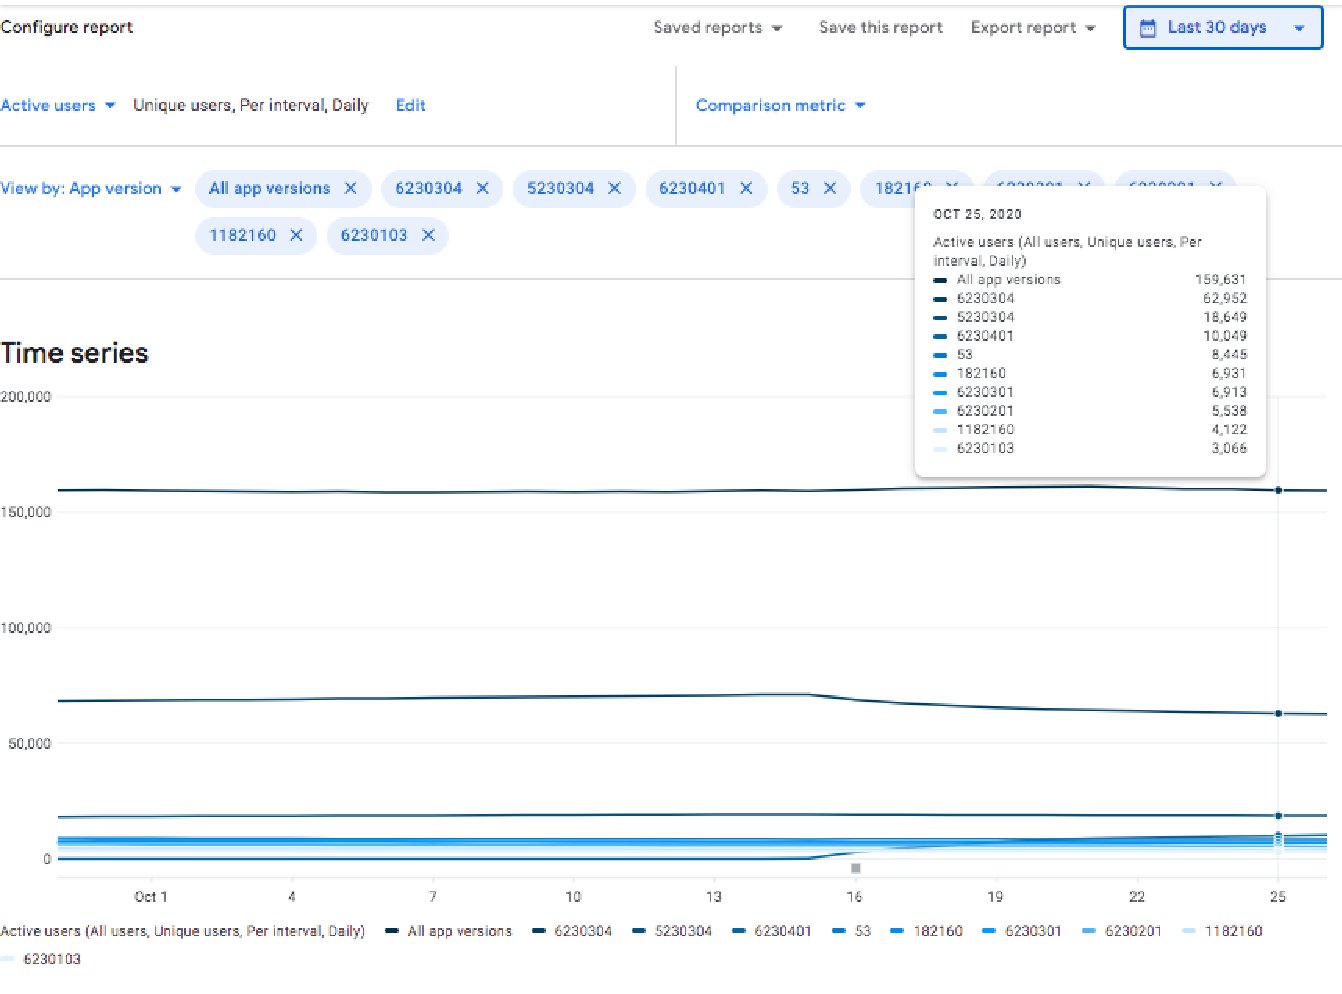
\includegraphics[width=\linewidth]{images/android-vitals-screenshots/kiwix/kiwix-ActiveUsers-30-days-2020-10-29.pdf}
    \caption{Kiwix Android Active Users 30 days by app version}
    \label{fig:kiwix-30d-active-users}
\end{figure*}

As mentioned above, there are various practical constraints to the frequency of releasing mobile apps using an app store. Chiefly there are two constraints: 1) the relatively slow rollout of new releases to the user-base which can take a week or more to achieve 50\% and also 2) the app store's review process which has been a hotly debated topic particularly by developers who may end up waiting days or even weeks for a release to be approved. Apple states~\emph{``Review times may vary by app. On average, 50\% of apps are reviewed in 24 hours and over 90\% are reviewed in 48 hours."} and Google informs developers in Google Play Console~\emph{``We're experiencing longer than usual review times
Due to adjusted work schedules at this time, you may experience longer than usual review times for your app."} ~\sidenote{This message is on the \texttt{app-dashboard} page for each app in Google Play Console and only visible to authorised development team members}. Sophisticated development teams may find ways to alleviate these constraints, for instance by shipping code updates that are applied by a current release rather than by creating and releasing a new binary of the entire app.

Given the constraints that are faced by the vast majority of mobile app developers, of rollouts taking many days and of needing to cope with sometimes lengthy delays in app approvals. 

Mention poor behaviour and their effects on app approvals.

TODO Discuss limits on releasing often that lead to an adapted set of working practices, release frequencies, etc. Perhaps do so elsewhere in this thesis?

\section{Mobile Analytics Usage Lifecycle}~\label{section-mobile-analytics-usage-lifecycle}
For projects that incorporate and use Mobile Analytics, it also has a usage lifecycle. It's important to recognise where the outputs come from, and then how they are interpreted, applied, actioned, and where and how the evidence can be obtained of the effects of applying results of the mobile analytics outputs.

\begin{figure*}
    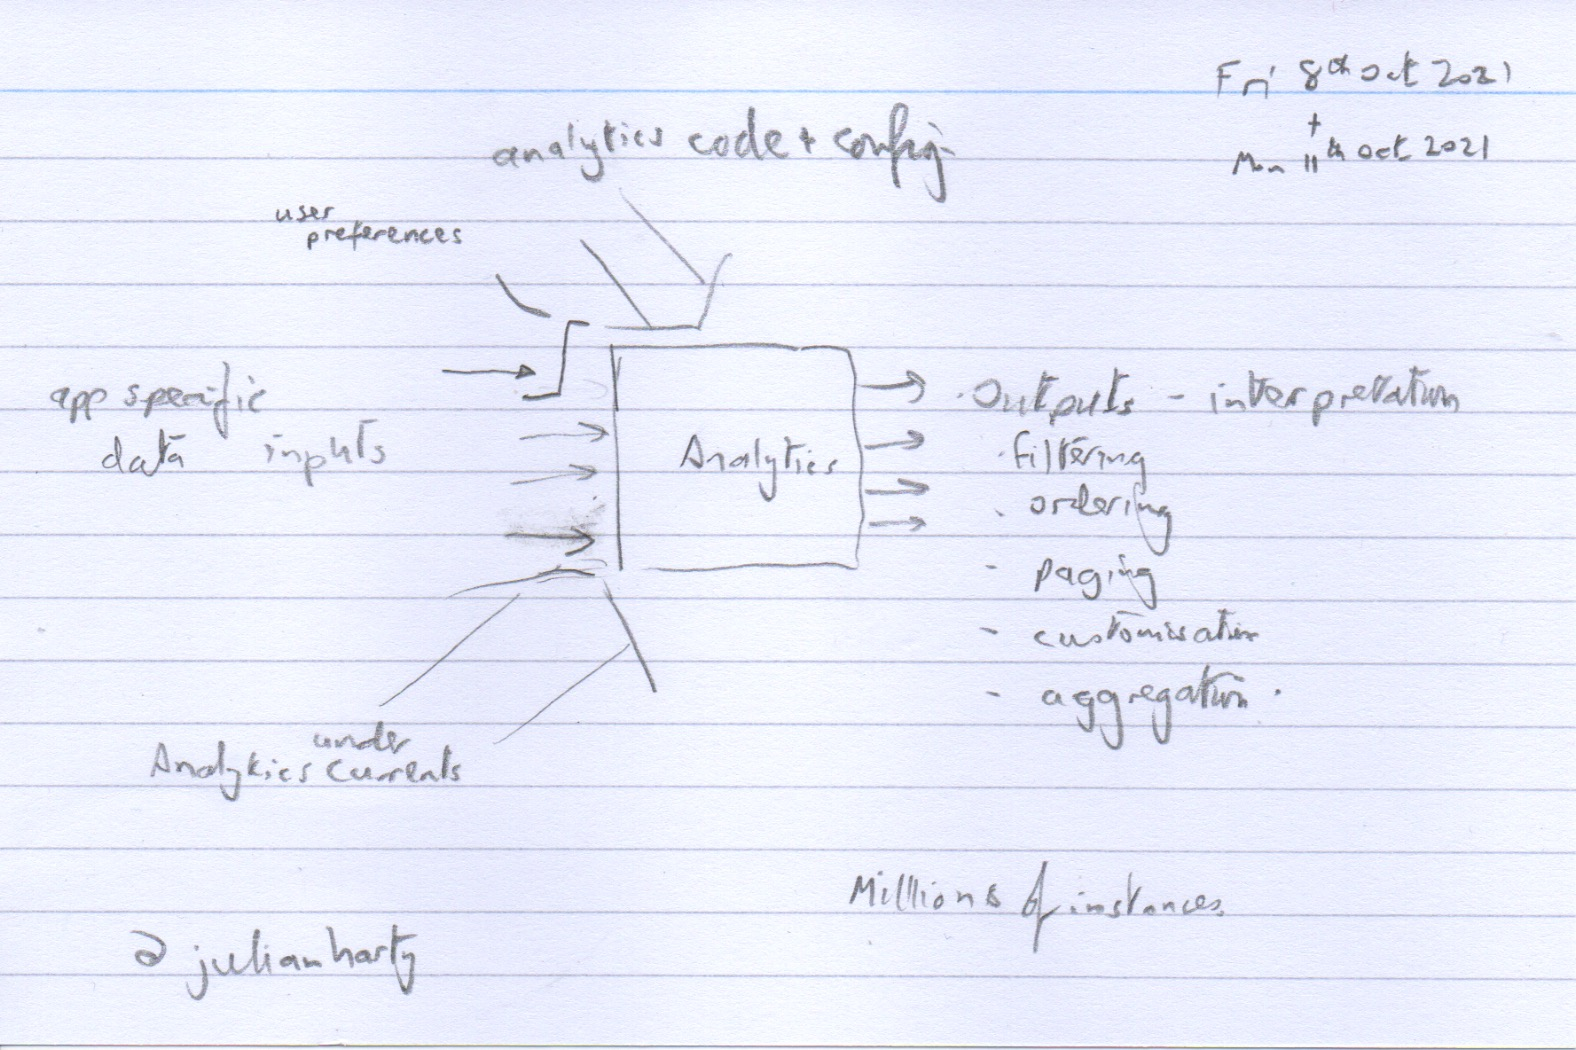
\includegraphics[width=\linewidth]{images/rough-sketches/outputs_from_inputs_code_config-11-oct-2021.jpeg}
    \caption{Outputs from Inputs, Code, and Config (draft)}
    \label{fig:outputs_from_inputs_code_config}
\end{figure*}

Figures \ref{fig:outputs_from_inputs_code_config} and \ref{fig:analytics-feedback-cycle} are connected and illustrate firstly what may affect the outputs pertaining to mobile analytics in isolation, and then how the contents of the first figure fit into a larger, holistic feedback cycle. 

\begin{figure*}
    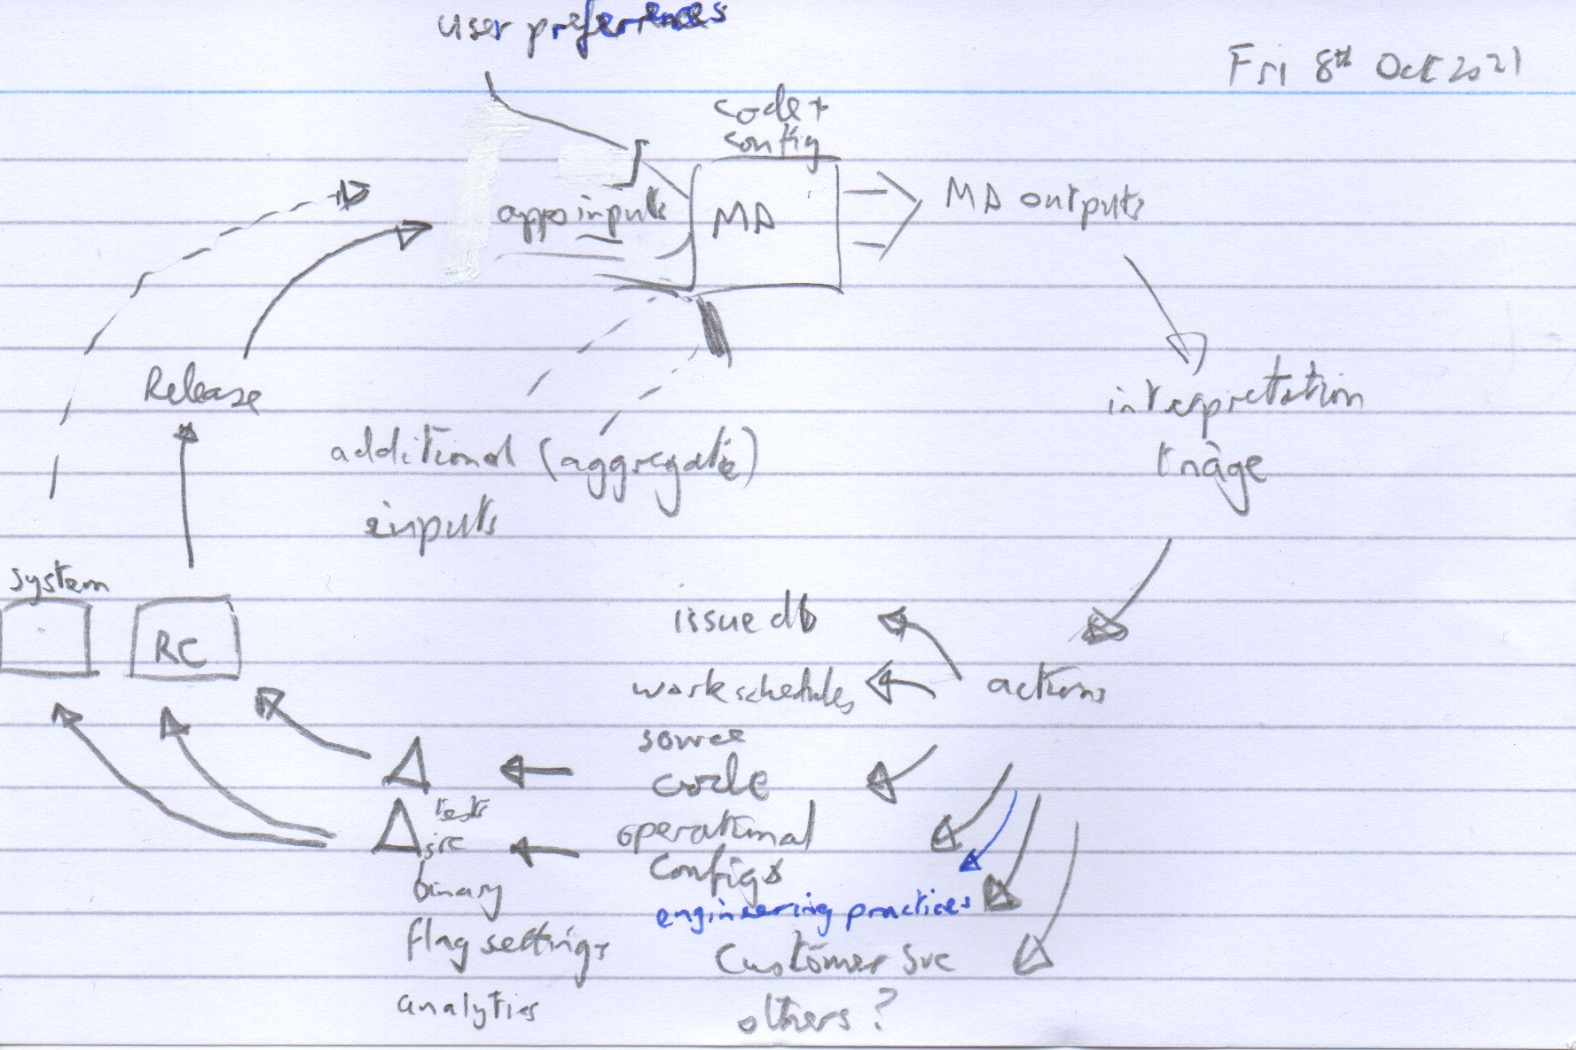
\includegraphics[width=\linewidth]{images/rough-sketches/analytics-feedback-cycle-11-oct-2021.jpeg}
    \caption{Analytics Feedback cycle (draft)}
    \label{fig:analytics-feedback-cycle}
\end{figure*}

In the first of the figures, \ref{fig:outputs_from_inputs_code_config}, working from right to left there is the interpretation of the outputs of a mobile analytics service~\sidenote{The service is provided to developer. It includes the code and configuration that are instantiated to provide analytics processing and reporting aspects; it excludes software running on the mobile devices.}. The interpretation is influenced by the various outputs and how they are used by whoever performs the interpretation. The analytics outputs are influenced by four elements: 
\begin{enumerate}
    \itemsep0em
    \item The service, which includes the instantiation of the server side code and configuration; 
    \item The app-specific inputs (such as failure data e.g. stack traces); 
    \item User-oriented preferences, settings, and so on (e.g. whether analytics reporting is enabled or blocked); and 
    \item Analytics undercurrents (the underlying data and sources may be unavailable to the developers however it may be used by the analytics service, for instance to provide peer-group reports).
\end{enumerate}

The figure illustrates the system for one app, however the analytics service may have as many as millions of instances e.g. Google Play provides one instance of the Google Play Console dashboard for each Android app live in the Play Store. \emph{The instances are unlikely to be identical; they may differ in the analytics code and configuration for instance if Google is running A/B experiments for Google Play Console or performing phased rollouts of new features and/or releases.} Developers may also have customised their analytics service, so they may have distinct views, reports, and interpretations than their co-developers and other colleagues.

In summary, the interpretation of what a mobile analytics service provides depends on the outputs which may, in turn, be affected by their navigation and use. 

The outputs are driven through a combination of elements; these are mainly outside the direct control of the developer, however the developer may be able to influence them. Examples of how the developer may be able to influence these include:
\begin{itemize}
    \itemsep0em
    \item Analytics code and configuration: the developer may be able to opt-in to early experience programs (EEP's), \emph{etc.} These may include new features, reports, and so on that are not available to developers who are not part of these EEP's.
    \item User preferences: the app may include facilities and/or guides aimed at encouraging the user to opt-in (or out) of providing analytics data.
    \item App-specific data inputs - here are some representative examples: the developer may be able to add additional calls to a suitable Mobile Analytics API, or to generate logging messages that are interpreted as failures by the mobile analytics client-side processing. Some Mobile Analytics APIs also provide programmatic access to discard analytics events at run time.  
    \item Analytics undercurrents: the developer may be able to select the peer applications and/or peer category their app is compared with.
\end{itemize}

As mentioned earlier, \secref{fig:analytics-feedback-cycle} subsumes \secref{fig:outputs_from_inputs_code_config} in the upper, central and right areas. Interpretation of the mobile analytics outputs is the first stage in being able to act on them. Triage is the next, and for those deemed sufficiently pertinent are likely to lead to actions. These actions may play out in one or more theatres, for instance in an issues database, in work schedules, in source code, operational configurations, and/or in engineering practices. They may also lead to actions in customer service, and others (such as user-oriented material \emph{e.g.} in online FAQs).

The actions may also result in changes to the sources for the mobile apps and/or in systems that support the app. Changes in the mobile app may form part of a Release Candidate (RC in the diagram) and subsequently in a release. If the release is deployed and then used it will provide fresh app-specific data inputs, and these then feed the mobile analytics.

\begin{figure*}
\RawFloats
\centering
\begin{minipage}{.70\textwidth}
  \centering
  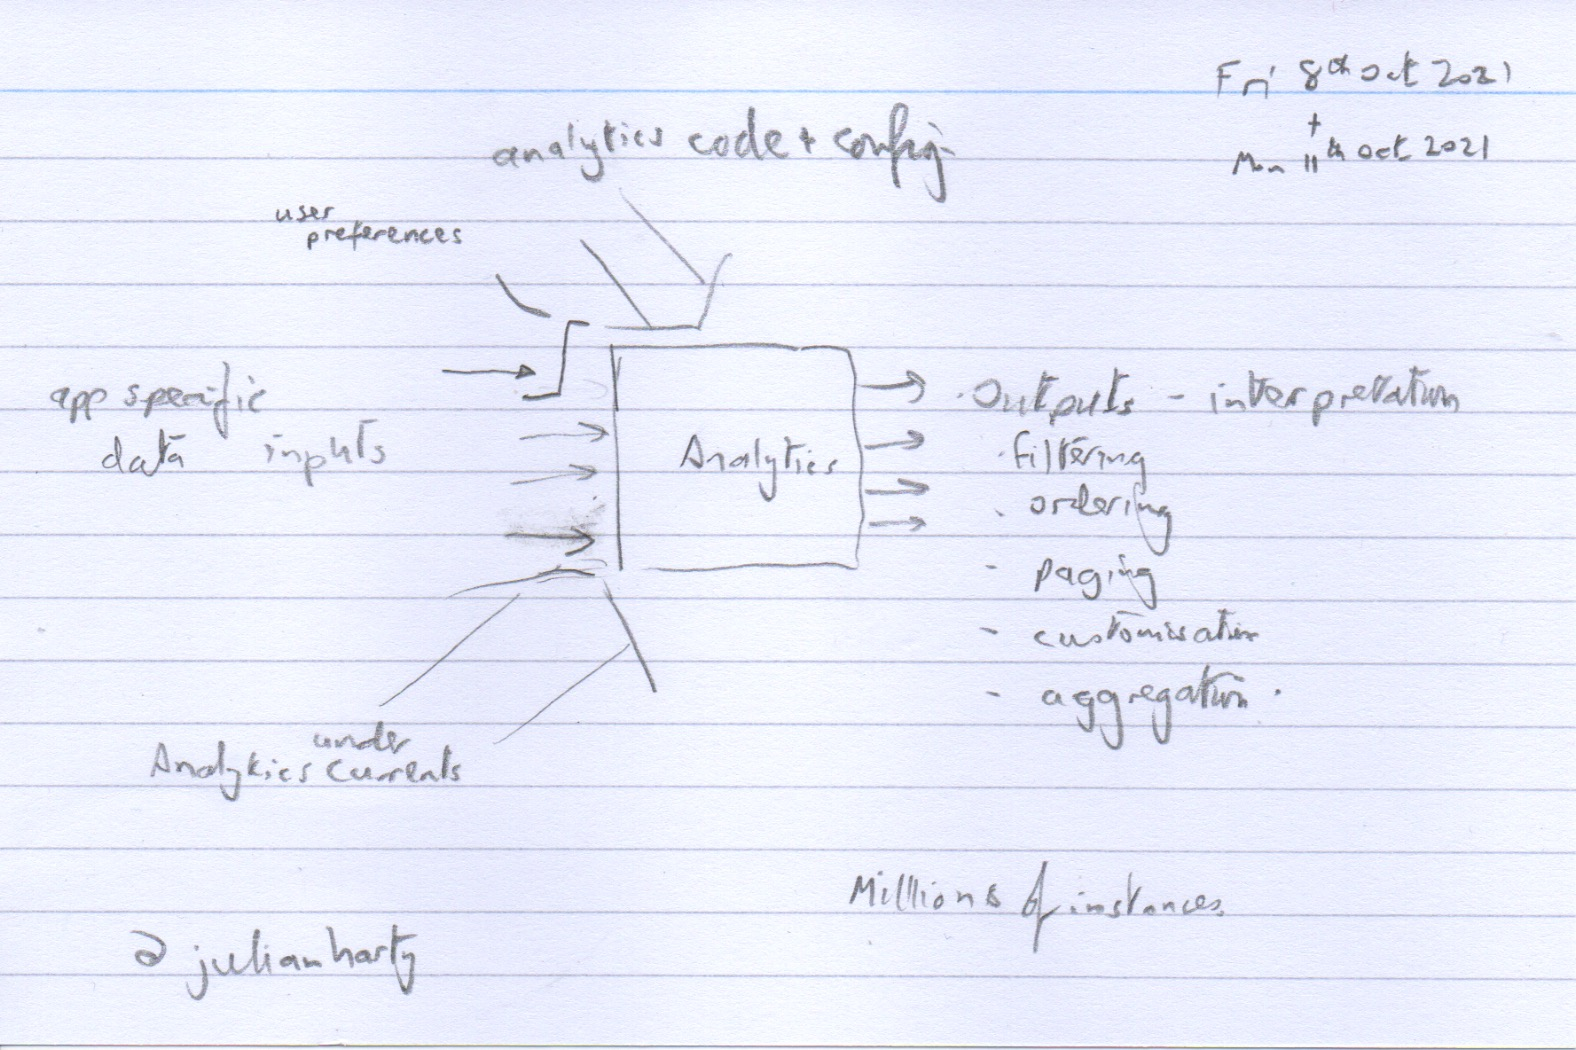
\includegraphics[width=\linewidth]{images/rough-sketches/outputs_from_inputs_code_config-11-oct-2021.jpeg}
  \captionof*{figure}{Outputs from Inputs, Code, and Config (draft)}
\end{minipage}\hfill%
\begin{minipage}{.70\textwidth}
  \centering
  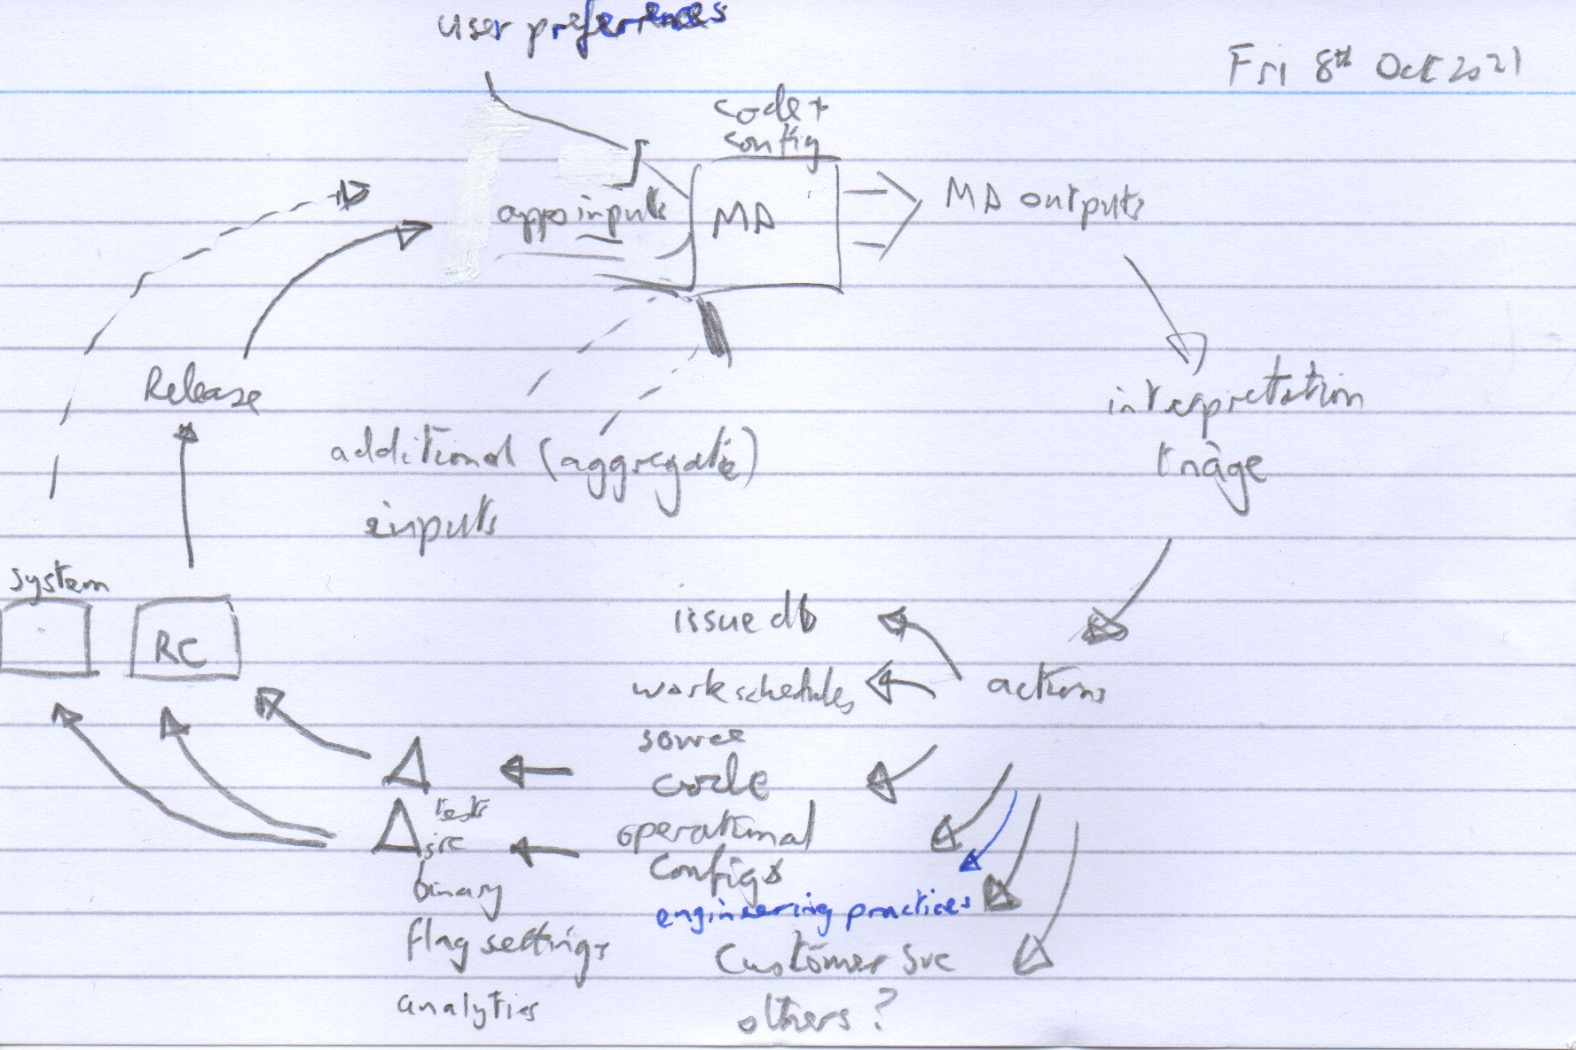
\includegraphics[width=\linewidth]{images/rough-sketches/analytics-feedback-cycle-11-oct-2021.jpeg}
  \captionof*{figure}{Analytics Feedback cycle (draft)}
\end{minipage}
    \caption{Mobile Analytics Contexts}
    \label{fig:mobile-analytics-contexts}
\end{figure*}


FYI: Figure ~\ref{fig:mobile-analytics-contexts} incorporates \secref{fig:outputs_from_inputs_code_config} and \secref{fig:analytics-feedback-cycle} and keeps the two figures together in the document. I've yet to work out if it'll work well with the text, it's here as a reminder I want to improve the links between these two related drawings.



\section{Information sources for app developers}
Developers want and need to know how well their apps are performing from various perspectives such as: growth and adoption (\emph{``do we have more users and are they using the app [more] often?"}), users' ratings and reviews (\emph{``do they like our work?"} and in terms of quality (\emph{``does it perform well? is it fast and reliable?"}). 

\begin{figure*}
    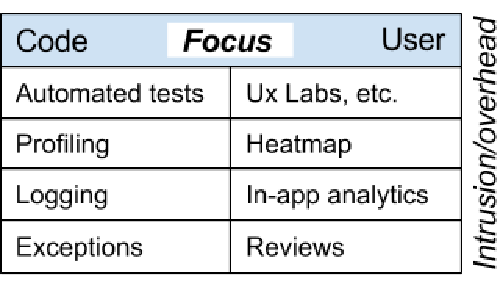
\includegraphics[width=\linewidth]{images/ComparingTechniquesRHS.pdf}
    \caption{Comparing Techniques}
    \label{fig:comparing_techniques}
\end{figure*}

\begin{table}
\RawFloats
    \parbox{.40\linewidth}{
        \centering
        \small
        \begin{tabular}{lll}
            Technique  & Gen. Effort & Usage Effort  \\
            \hline
            Automated Tests  & High  & Medium \\ 
            Profiling   & 1 & 1 \\
            Code Quality tools & 1 & 1 \\
            Logging   & 1 & 1 \\ 
            Exceptions  & 1 & 1 \\ 

        \end{tabular}
        \caption{Focus: Code \label{HRVtable}}
    }
    \hfill
    \parbox{.40\linewidth}{
        \centering
        \small
        \begin{tabular}{ll}
            Technique & vector$_1$  \\
            \hline
            UX labs, etc. & 1  \\ 
            Heatmap & 1  \\ 
            In-app feedback & 1  \\ 
            App-store reviews & 1  \\
        \end{tabular}
        \caption{Focus: User \label{BACtable}}}
    \caption{Comparing techniques}
\end{table}

HRV data in Table \ref{HRVtable} and BAC data in Table \ref{BACtable}.

There are various techniques that can be used to assess aspects of quality of mobile apps. Figure \ref{fig:comparing_techniques} provides a visual overview of eight techniques. Of these four are code-oriented and the remaining four more user- or usage- oriented. They are ordered in approximate rank of the overhead, effort, or intrusion involved of each technique. % MUST-DO continue and expand this argument. Discuss why exceptions were chosen as one of the core elements of this research and PhD thesis.

Google's Google Play app store provides developers with answers to all these niggling questions through a developer-oriented user interface called Google Play Console. 
In Google Play Console they provide various tools, reports and data all aimed at informing developers about how their apps are 'doing' and performing. Broadly, these include an overview page with one line of pre-selected data per app managed by the Google Play \textit{Developer Account}. Then, per app, Google provides an overview dashboard of graphs which, in turn, link to more detailed reports and information which provide greater depth. (Examples are provided in the~\href{appendix-analytics-tools}{\emph{\nameref{appendix-analytics-tools}}} appendix.)  Some graphs only appear when Google's algorithms decide they are relevant, these seem to be related to events and/or volumes of underlying data.




\section{Passive, tacit, and explicit analytics choices}
Various degrees of choices are available depending on how actively the development team wishes to incorporate analytics into their development practices. These include using what already exists, where the data is gathered by others and made available to the developers, here these sources are called \emph{passive analytics}. Developers can choose to take more authority in the data collection, for instance by deciding what data they would like to collect and how they wish to collect it. They can use these tools at various depths, ranging from superficial use to actively maximising the efficacy of using analytics to provide them with the data they believe they need to achieve their outcomes. There is an interesting discussion in a blog article~\sidecite{mukherjee_implicit_versus_explicit_event_tracking_hits_and_misses} on what they term \emph{implicit, or codeless} and \emph{explicit or code-based} event tracking using web analytics tools. The article compares the benefits (hits) and flaws (misses) of both approaches. It also provides a flow chart to help teams select analytics tools that suit their context.

% More reading
% https://web.archive.org/web/20120401053907/http://www.wiikno.com/blog/explicit-vs-implicit-data
% MUST-DO check Patrick's recording of this webinar: https://snowplowanalytics.com/events/explicit-vs-implicit-tracking/ and write up germane items here.


\subsection{Passive Analytics}~\label{subsection-passive-analytics}
Passive analytics are those not actively under the control or influence of the development team, they are provided from other sources such as the operating system or the app store. In the context of this research the passive analytics are all managed by the app store, Google Play, and made available to developers through Google Play Console. As Google states in a US patent,~\emph{``several services provide passive analytics collection such as receiving information about the device type, time of usage, location usage, feature usage, and event reporting."}~\sidecite{googlepatent_hyman2016_collecting_application_usage_analytics}.  

% COULD-DO compare with the concept of passive monitoring https://en.wikipedia.org/wiki/Passive_monitoring however the Wikipedia article doesn't currently add enough to justify citing it or comparing with it.

\subsection{Tacit Analytics}~\label{subsection-tacit-analytics}
Tacit is variously defined as \emph{``Something tacit is implied or understood without question."}~\sidenote{\url{https://www.vocabulary.com/dictionary/tacit}}, \emph{``Understood or implied without being stated."}~\sidenote{\url{https://www.lexico.com/en/definition/tacit}, Note: Lexico.com is a new collaboration between Dictionary.com and Oxford University Press~\url{https://www.lexico.com/about}}, silent, wordless, or noiseless. 
%
It may be something that is inherent in the nature of using many of the third-party analytics libraries. In this research~\emph{tacit analytics} is where developers accept whatever default data is collected by an analytics library without the developer needing to do anything more than integrate the library into their app. 

\subsection{Explicit Analytics}~\label{subsection-explicit-analytics}
Explicit analytics is where developers have actively added code to interact with analytics libraries, for instance by calling methods in the API(s) provided by the library's. There are various degrees of use of the APIs and developers may have various intentions for calling these APIs.

\section{Drilling down into analytics}\label{section-drilling-down-into-analytics}
At the highest level of information, an item and an associated number provides some information: a total crash rate of 99.1 \%, 97K total installs, 37 reviews, and so on. These values may change over time, however if we do not keep track of previous values they cannot be compared, and also relevant information may be hidden behind the totals. The total sums up as many values as exist (from zero values onwards). Some of the reported analytics are of this high-level form.

Totals for subsets of the overall volume of data helps provide additional and potentially relevant information. Relevant subsets for mobile analytics include: date ranges, app releases, platform versions, and many others. Other examples, found in some analytics tools include crash clusters - collections of crash reports considered to be sufficiently similar to enable various individual crashes to be grouped and aggregated. The ability to segment and report on segments allows more detailed analysis than simply observing subsets. 

Comparisons with one or more peer groups provide relational analytics, helping answer: ``how is this app performing compared to various peer groups?" Unless the team has direct access to the data for their peer group, the statistics for the peer group need to be available to a trusted party who perform the comparisons. Some data is publicly available for instance the overall rating of an app together with a limited number of recent reviews and the total installs \textbf{MUST-DO} write up research that uses these sources in the related works chapter, add some of the citations here. There are also commercial services available, and some analytics tools, including Google Play Console, provide these comparisons as part of their services.

Individual records provide the most detail that's available. Note: Developers may be able to create new records and enhance existing records and/or add additional forms of analytics if they want/need more detail. Examples of individual records include stack traces for crashes and similar internal state data for ANRs. Some analytics tools allow developers to capture and subsequently see individual records, for instance details of an item added to an e-commerce shopping cart by an end user. Mobile analytics ultimately can only report on data that is provided to it. 

The analytics tool may or may not make aspects of the data available to the users of the tool. As a concrete example, Google Play Console provides developers access to individual reviews (with their associated rating), it also used to provide access to crashes and ANRs for several years before removing these and replacing them with summary data in 2018 \textbf{MUST-DO} add reference and cite it.

\textbf{MUST-DO} provide screenshots of category peer groups and custom peer groups. Discuss either here, or in a later chapter, Google's cap on the number of changes to the custom peer group.

Two key points in summary: being able to keep track of analytics as they change over time allows comparisons and trends to be determined. Additional detail can help identify meaningful differences for instance that a crash rate is much higher than the mean for a particular model of smartphone. 

How much information is needed to be actionable? (Thought: This may be more of a research question...)


\textbf{MUST-DO} introduce my concept of resolution.

\textbf{PERHAPS} introduce the concept of app peer groups here?


\section{Summary and transition}
% This chapter has introduced various concepts and topics which help provide context for the rest of this thesis. Some additional background material is available in various appendices, including more information on mobile analytics and various software contributions.
We now have a grounding in the domain of mobile apps, logging and mobile analytics which is underpinned by research in both academic research and grey literature. The next chapter describes the application of mobile analytics to software development practices for mobile apps.
\setkeys{Gin}{draft=false}
\setchapterpreamble[u]{\margintoc}
\chapter{Related Work}
\label{chapter-related-work}
\epigraph{I recall seeing a package to make quotes}{Snowball} % https://tex.stackexchange.com/a/53378/88466

% Additional, older material is online in https://docs.google.com/document/d/1OdoBsLboTZHzv1UP9g7nUriVLgpu6ZGqjXLmRAAlAfs/edit?usp=sharing
% New ideas and material are being added to a Google Doc for a while, then I'll revise this chapter. https://docs.google.com/document/d/1i3cCk2-8zwVioAuMbBQDLcUViihhHY6gk0MJNPevFbA/edit?usp=sharing

\begin{figure}
    \centering
    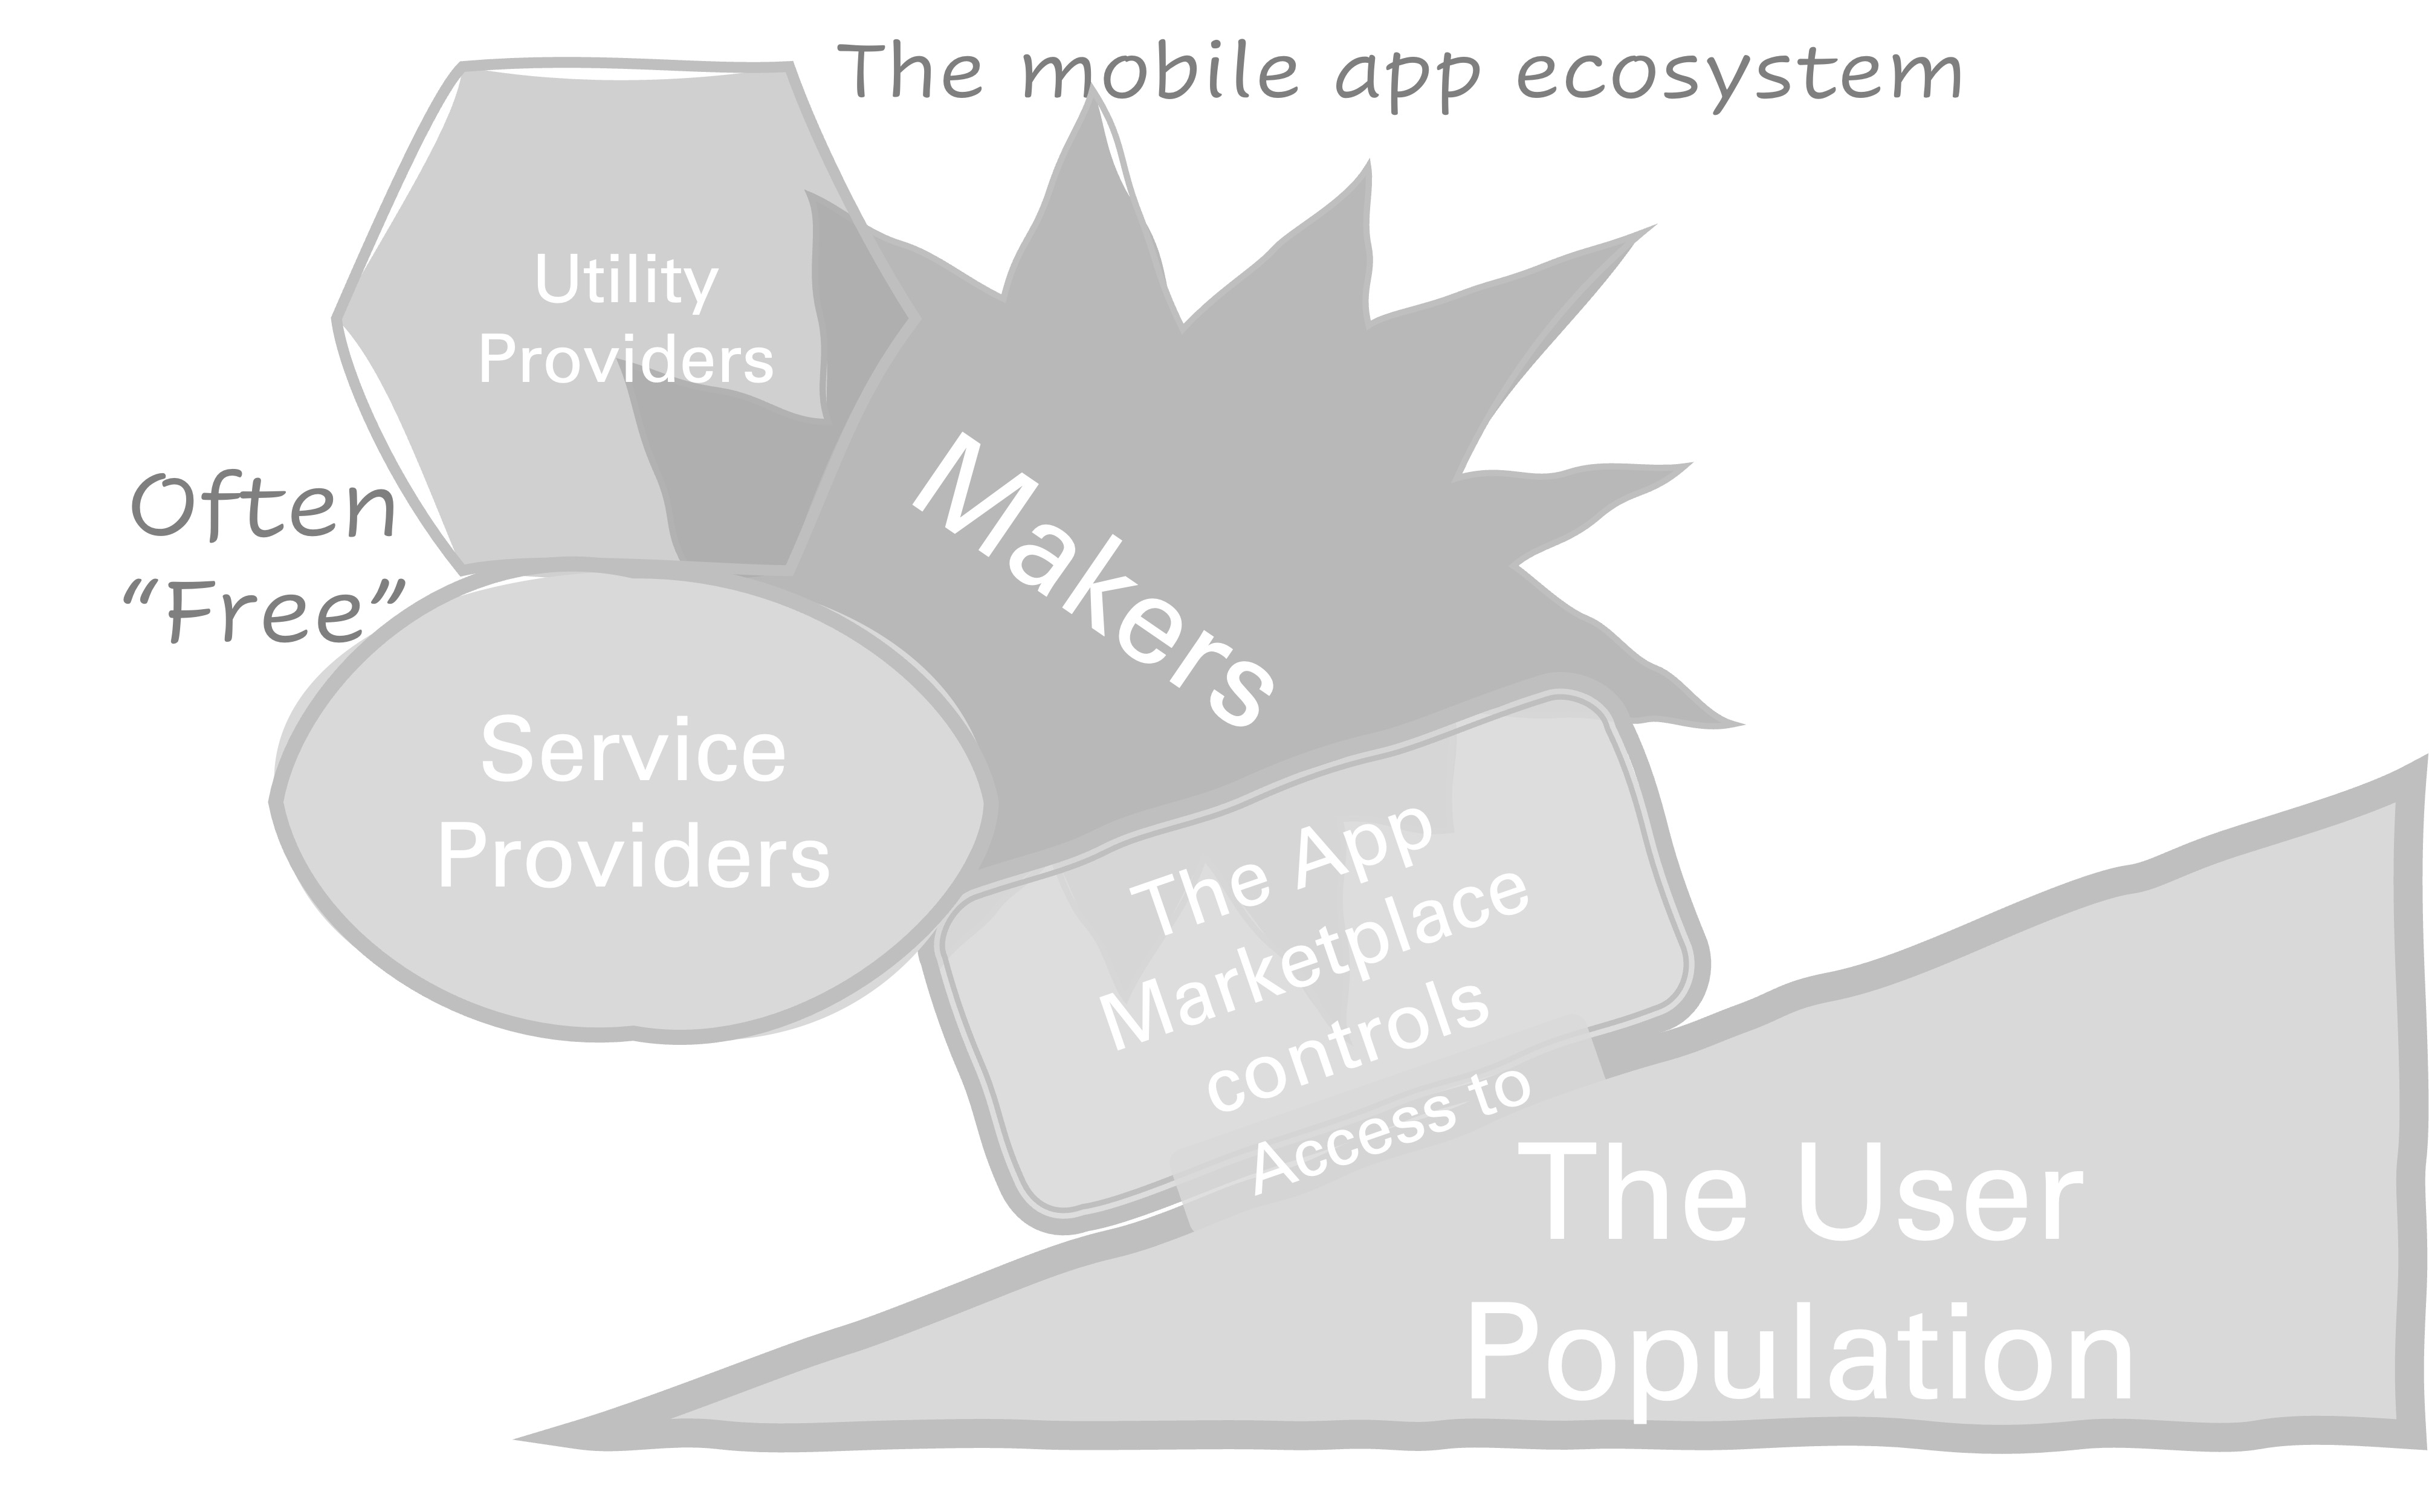
\includegraphics[width=\linewidth]{images/my/the-mobile-app-ecosystem-27-jul-2022.jpg}
    \caption{The Modern Mobile App Ecosystem}
    \label{fig:my_modern-mobile-app-ecosystem}
\end{figure}

The modern mobile ecosystem, illustrated in Figure~\ref{fig:my_modern-mobile-app-ecosystem}, 
sets the context for the thesis and this chapter together with the research questions. The marketplace - the app store - establishes the ecosystem which generates revenues from the user population and frequently to a lesser extent from the makers -  the developers of the apps. Various providers of utilities and services offer these to the makers and they may also obtain revenues from one or more parties that are part of the ecosystem and/or from others, including advertisers.

My work nestles within the works of many people in various related fields: in software quality, in analytics, and in the mobile device ecosystem. As researchers we understand and recognise there are gaps in the current state of the art, this chapter aims to identify several pertinent gaps which led to this research being performed, \emph{i.e.} which motivated me to act. The mobile ecosystems touch on billions of people's lives, where flaws in the apps and the ecosystem can adversely affect the lives of many of those people. 

Research in how mobile apps are created and tested, the relevance of app stores, service and utility providers, the user bases for mobile apps within the overall population of users of an app store ecosystem are all relevant. And meanwhile understanding why it's hard to create reliable software is also vital as part of acknowledging some of the grim realities development teams need to face if they are to succeed in their other goals and objectives for their mobile apps. An understanding of research into how to measure software qualities, and stability in particular, is key to establishing ways mobile analytics measures these qualities. 

At times this chapter will draw from broader sources, for instance in software development, testing, and analytics as these provide context for the particulars of the mobile app ecosystem. Conversely, in my view, and based on discussions at a peer workshop in Japan~\sidecite{nii_shonan_workshop_152}, I proposed a model, shown in Figure~\ref{fig:my_shonan_hysteresis_sketch}, that seemed to be well accepted and became part of the formal post-workshop report~\sidecite{nii_shonan_152_workshop_report}, where the mobile ecosystem is influencing the desktop app ecosystems. Examples include: app stores, per user licensing across multiple devices, public ratings and reviews, platform (device) level, crash reporting, and usage analytics, and so on.

\begin{figure}
    \centering
    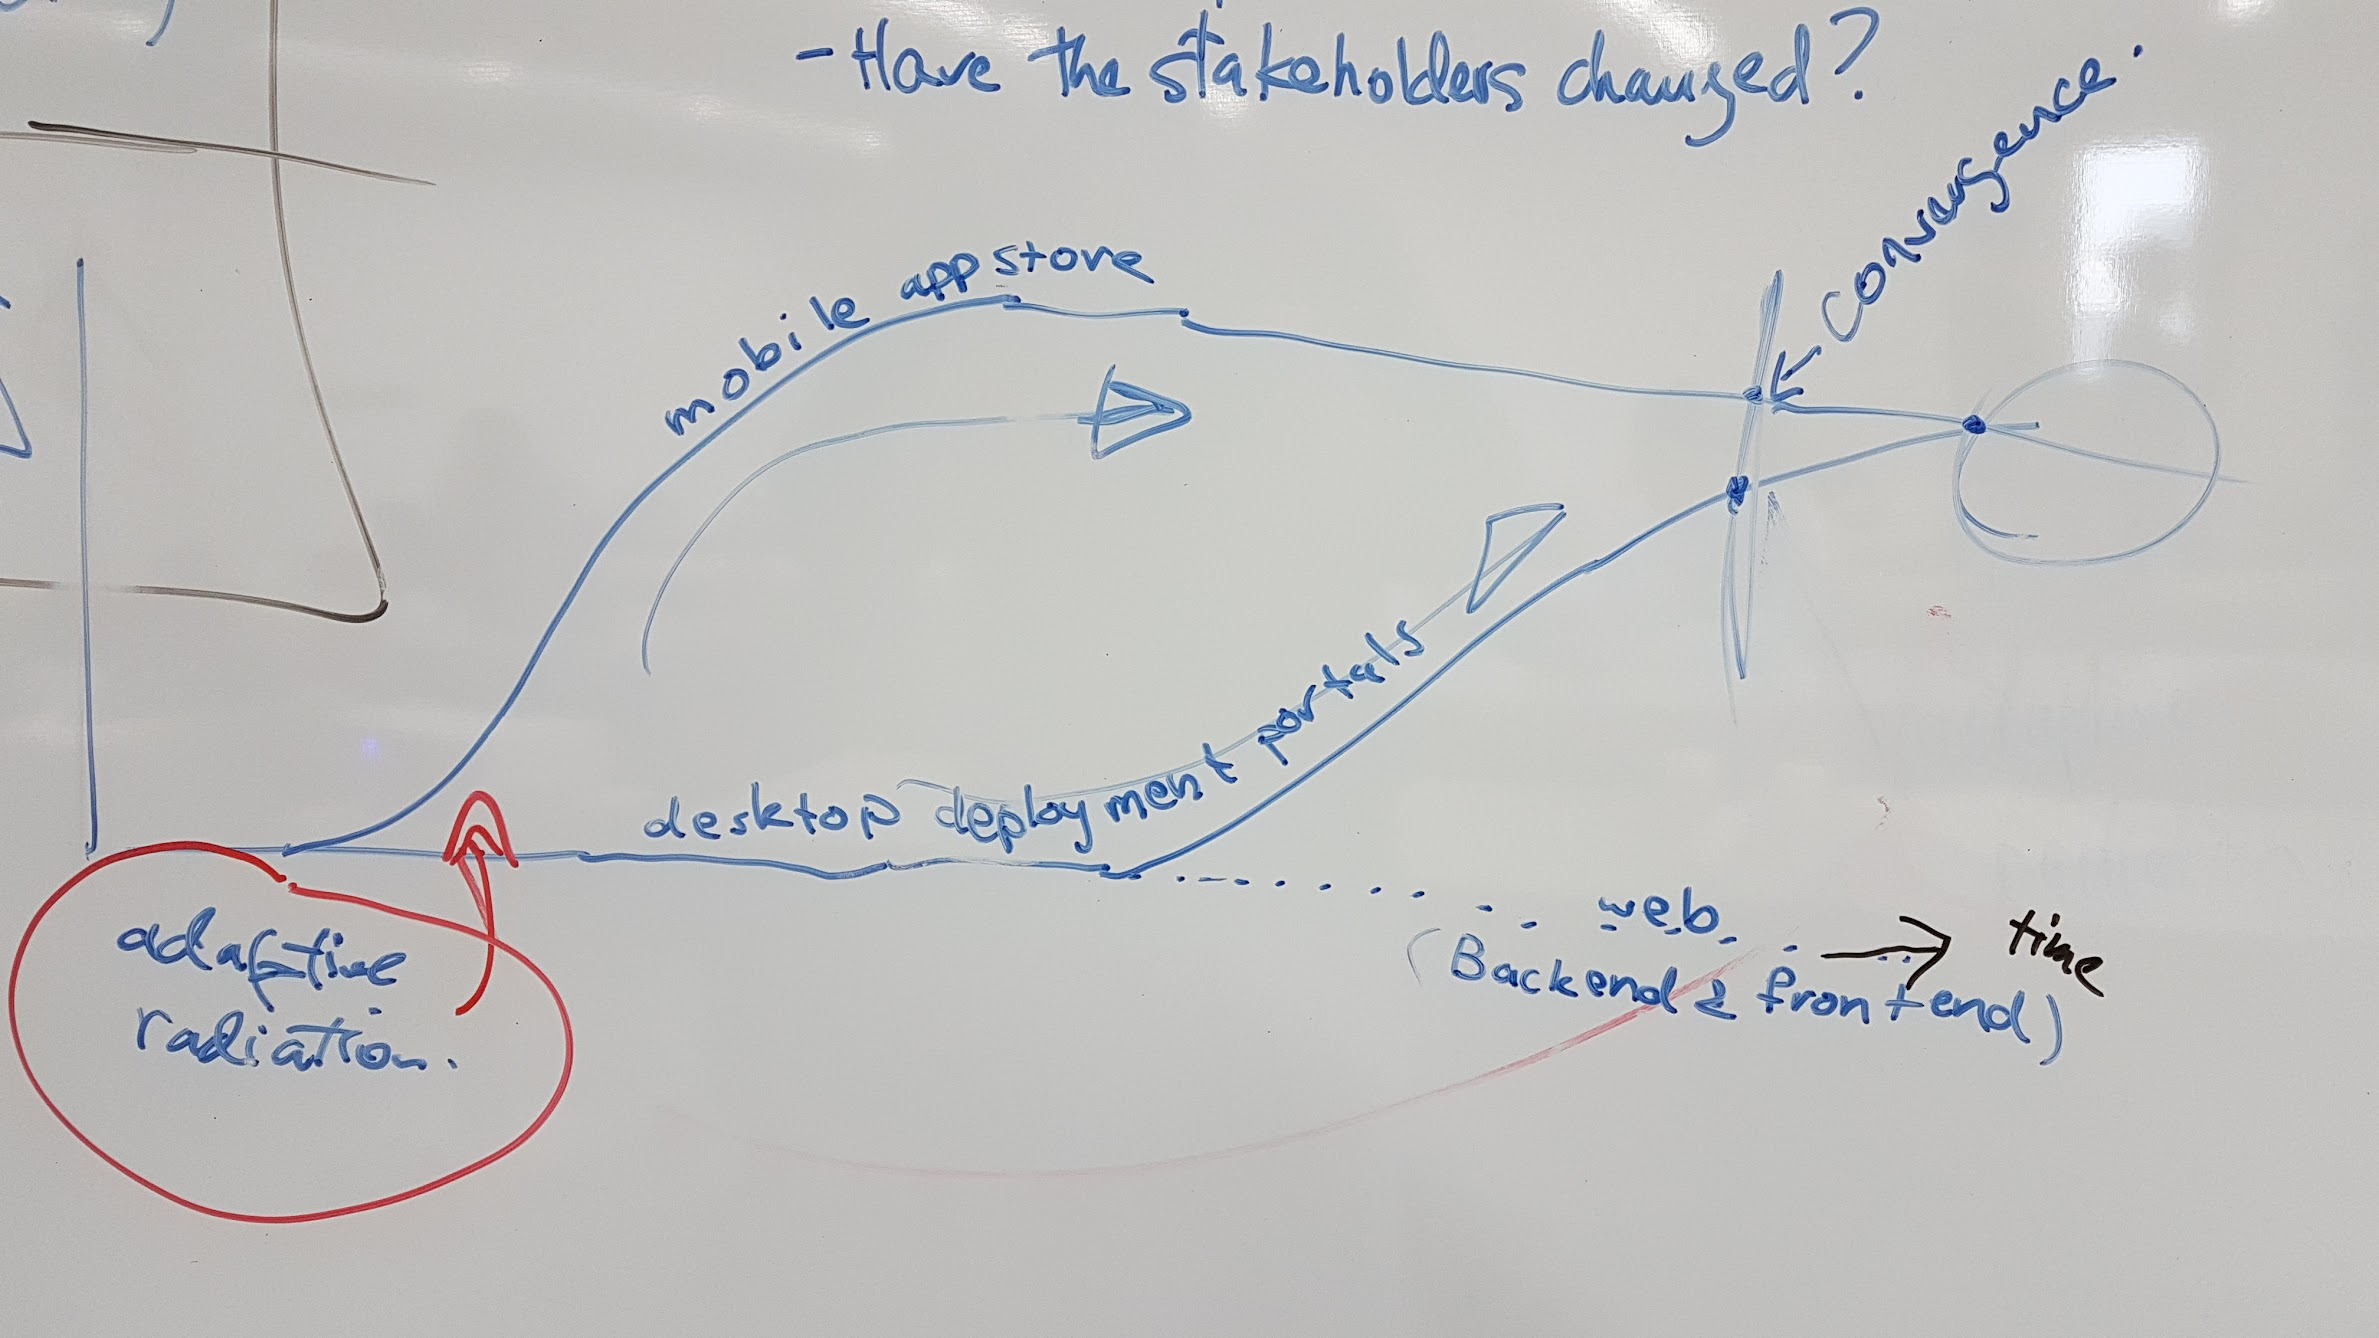
\includegraphics[width=\linewidth]{images/nii-shonan-workshop-152/shonan_hysteresis_diagram_20191210_132528.jpg}
    \caption{Mobile and Desktop Growth and Convergence}
    \label{fig:my_shonan_hysteresis_sketch}
\end{figure}

If the mobile ecosystem is influencing other ecosystems, perhaps this research will also apply to those ecosystems, albeit there are likely to be many distinctions as each ecosystem is distinct and unique.

\newthought{A note on the choice of ecosystem}: 
The practicalities of the research and the case studies where nearly all the work pertains to the Google Android ecosystem also helps in the selection criteria of relevant related works. As the vast majority of active research in the domain of mobile apps also pertains to this ecosystem, this means the topic is richly served in terms of related works.

\newthought{Contents of this chapter}:
The next section provides an overview of the methodology for this chapter, this may be removed pre-submission, nonetheless it is intended to help explain the rationale and the method that underpins the research into related work.

Subsequent sections are organised to provide the context of the research. There are two strands of existing research that this research builds on The first strand comes from software development generally in terms of: development practices, software quality, including measuring software quality, and then the use of software analytics. The second strand is the app store ecosystem and the effects it places on software development and engineering.

These two strands both affect development practices when developing, testing, releasing, and maintaining mobile apps. A particular aspect of developing mobile apps - feedback - is further developed in terms of the feedback that's available to app developers and the research into several of these forms of feedback. The final topic is existing research into crashes and freezes of mobile apps - these are both indicators of poor quality-in-use of the mobile app.

\begin{figure}
    \centering
    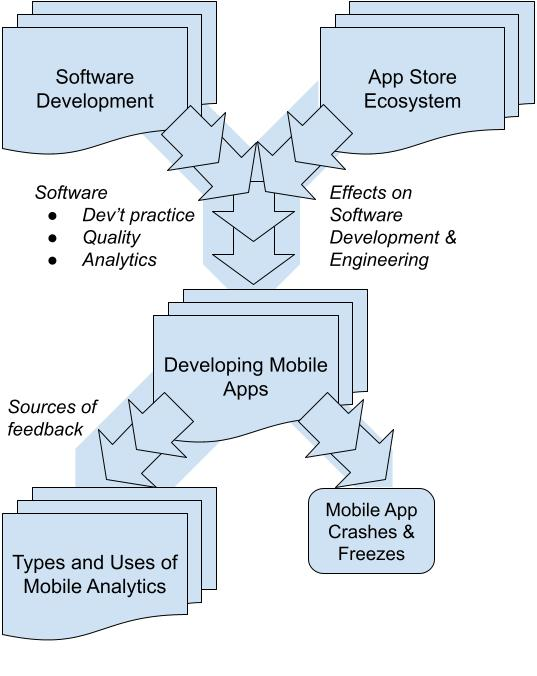
\includegraphics[width=\textwidth]{images/my/related-work-chapter-structure-27-jul-2022b.jpeg}
    \caption{Structure of this related work chapter\\ Source: \href{https://docs.google.com/drawings/d/1DosM__BfTGqoIYkkkltbyDreCT5wYC1Z0mR9i1ZSxWc/edit?usp=sharing}{Google Drawing}, access limited to collaborators to this thesis.}
    \label{fig:related-work-chapter-structure}
\end{figure}

% Reinstate the following once I've completed the first complete draft of the following sections.
% starting with research into app stores and their effects on software development and engineering \ref{rw-app-stores-and-their-effects-on-software-development-and-engineering}...

\section*{Notes on the proposed tactics and topics for the related work chapter}
Marian suggests I aim for writing brief, one-paragraph summaries and apply the T tactic of the broad literature, the top bar of the T are the many and various papers on a topic, and I'm picking these ones that are most directly germane to my research which become the vertical bar of the T.\pending{I'm still currently more verbose than this :(} 

Marian also suggested I might end up with two or a maximum of 3 levels of Ts. The higher level would be on Software Quality Improvement. The lower level would be on mobile analytics.

Where others have done similar work they've done so in other ways eg MSR rather than focusing on the development teams. When I observed the teams the effects of the processes, artefacts, and the tools emerged. This is why I've picked these 3 aspects and 6 perspectives. 

\subsection*{Some notes on the methods used for the literature review}

\begin{figure}
    \centering
    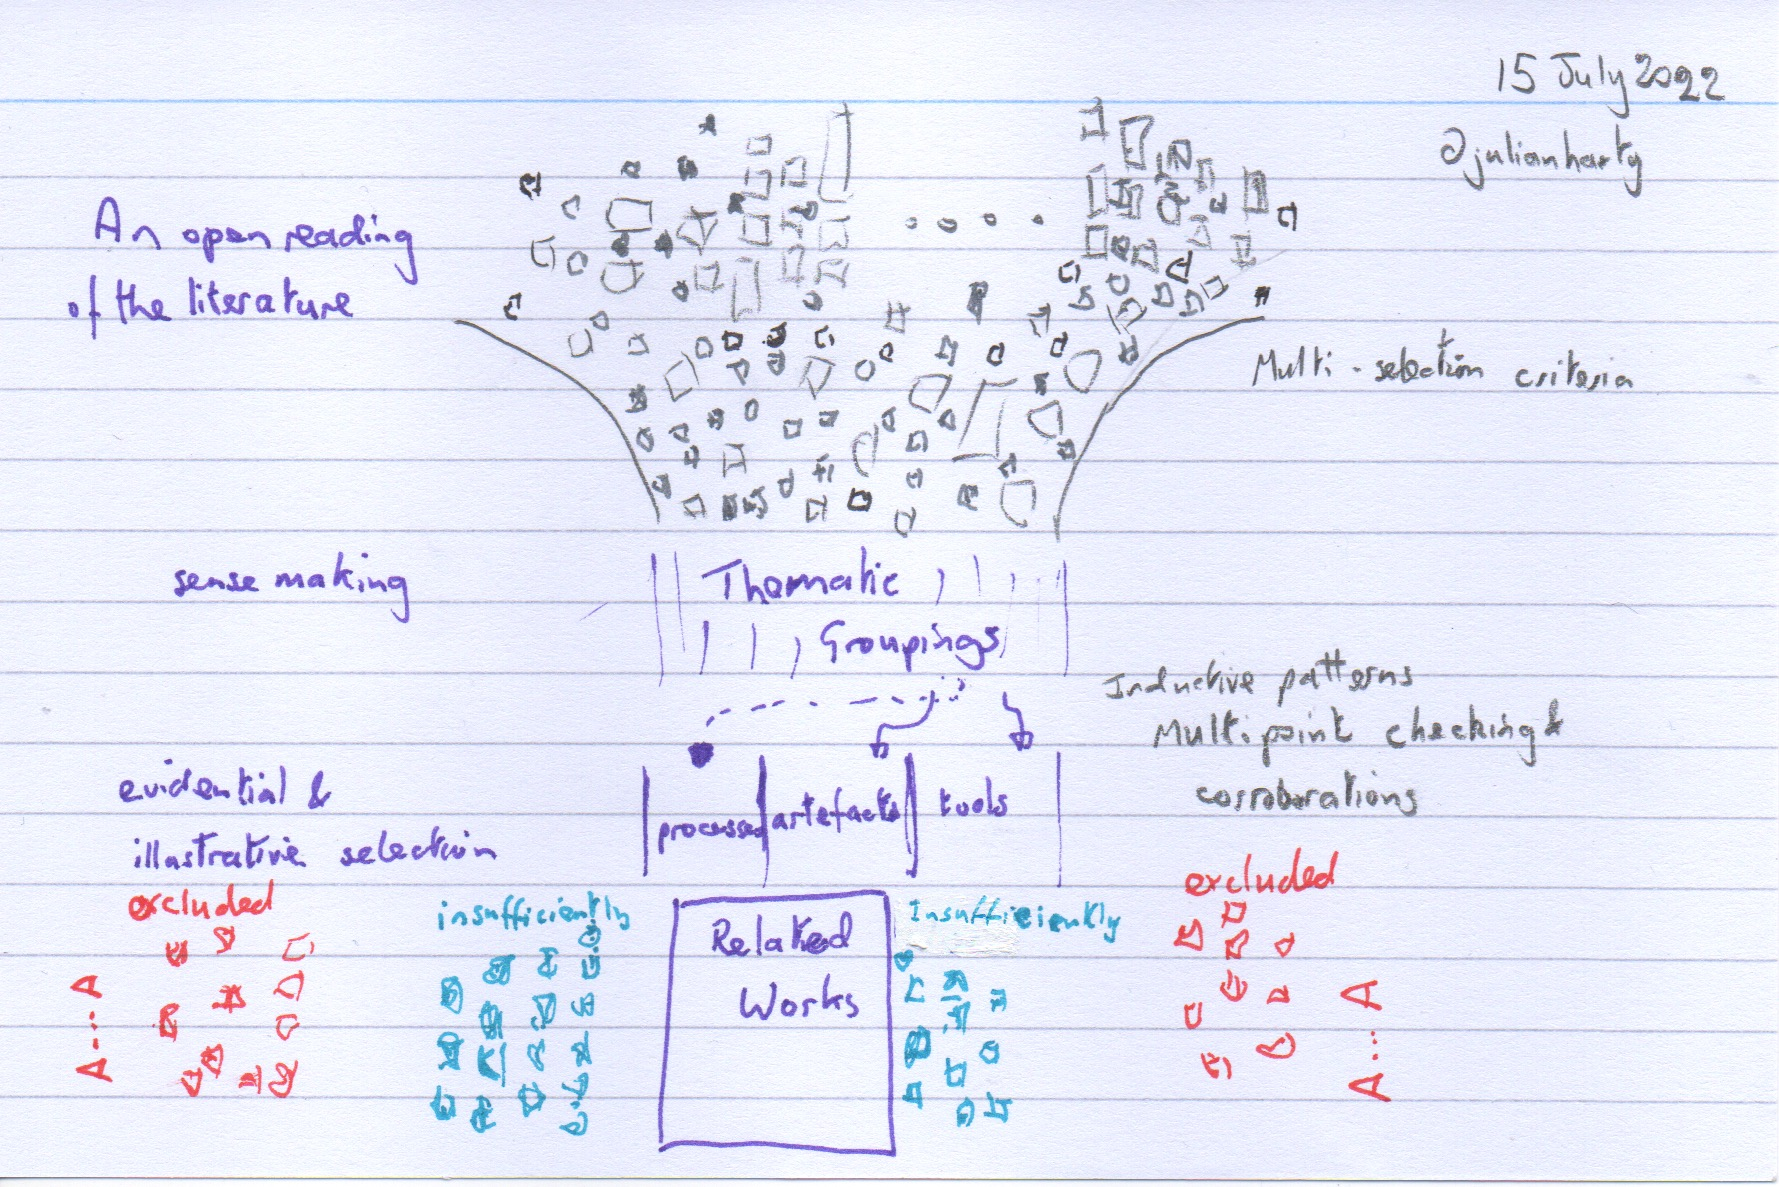
\includegraphics[width=\textwidth]{images/rough-sketches/literature-review-overview.jpeg}
    \caption{Overview of the literature review process and outcomes}
    \label{fig:literature-review-overview}
\end{figure}

Figure \ref{fig:literature-review-overview} illustrates my approach to researching prior work in the use of mobile analytics by app developers in order to measure and improve the stability/reliability of their mobile apps in the field/in the wild. Various searches, including keyword, tags, and related items, were incorporated into the searches. Initial sources included Google Scholar to find the more research oriented materials and Google Search particularly for grey materials, helped provide initial material to seed further searches. Specialist search tools were used where sites provided them, for instance on stack exchange sites such as StackOverflow, GitHub.com, acm.org, ieee.org, and medium.com their respective search engines were used frequently. Where practical copies of material has been preserved privately and backed up using at least one commercial, paid-for, cloud file storage service.

Multi-selection criteria are used to select material that appears of interest, relevant, and plausible. Generally bibliographic entries were obtained and these where checked for accuracy and completeness. Grey material seldom has a bibliographic entry, these were created, generally by hand, and preserved.

Through a process of sense-making, cross-checking, and corroborations various thematic groupings emerged together with potential relationships between the thematic groups. On reflection three clearly distinct and vital aspects emerged in the related work - the development practices used by mobile app developers, the artefacts they create and maintain, and the mobile analytics tools the developers use. These were further refined into six perspectives, using a three-by-two matrix: the x-axis incorporates the three aspects of processes, artefacts, and mobile analytics tools; the y-axis focuses on the current \emph{what is}, and \emph{what might be} in terms of making improvements.\pending{Arosha suggested three pillars which sounds good.}

The research materials and the bibliographic entries are maintained online. The most relevant ones are included in this thesis, many more are maintained in an `outtakes' folder, for example as `fieldstones'~\citep{weinberg2006weinberg} or in an insufficiently-related-works chapter. There's also an `excluded biography' file which helps reduce unnecessary repetition or groundhog day like practices. In the figure (\ref{fig:literature-review-overview}) the two \texttt{A ... A}'s wraps around - excluded works and insufficiently related works are similar distanced to this related works chapter.

In reading the literature various \textit{false friends} emerged, papers that first appear relevant because of their titles and/or abstracts but turn out to be on very different topics. 
Knowing about the concept of false friends and having pragmatic strategies to deal with them is important to avoid misunderstandings or misleading application of their work, 
based on \citep[p. 1833]{chamizodominguez2002_false_friends_their_origins_and_semantics_in_some_languages}. 
\citet{shaw1989_comparing_conceptual_structures__consensus_conflict_correspondence_and_contrast} uses the term 'conflict`, where, \emph{``experts use [the] same terminology for different concepts"}~\citep[p. 3]{shaw1989_comparing_conceptual_structures__consensus_conflict_correspondence_and_contrast} (and, indeed, using their terminology here there is a `correspondence' where experts use two terms to describe the same concept e.g. `false friends' and `conflict' both describe the same concept.). For this research my work was limited to recognising false friends and identifying some examples. 

So somehow I should aim to have the chapter structured with the following topics:\pending{This is a note to myself and needs replacing as I refine the chapter.}
\begin{enumerate}
    \item \textbf{Software Quality [Improvements] for mobile app developers}: Software Quality has been a contested topic for decades with no single accepted coherent agreement on what form(s) it takes, how software quality is measured, etc. Then comes the similarly vexed challenge of determining the concept and application of improvement in the quality/qualities of software. 
    \item \textbf{Mobile Analytics}: Research into \textbf{Processes, artefacts, and tools} necessary when using mobile analytics for improving software quality/qualities. These groupings emerged during the analysis of the literature and through understanding the practices of app developers.
    \begin{itemize}
        \item \textbf{Processes}: a.k.a. Analytics in Use - research into the processes developers use when they use mobile analytics
        \item \textbf{Artefacts}: things the developers create and maintain as part of their development work. Some of these are generated, in particular the app binary that is destined for end users once delivered by the app store.
        \item \textbf{Mobile Analytics Tools}: that the app developers use are worth researching in order to learn about their characteristics.
    \end{itemize}
\end{enumerate}

\subsection*{Software Quality Improvements for mobile app developers}
Here topics might include the measures that have been used by app developers to measure software quality - as confirmed by research literature and grey materials. I suspect this is where I'd include sources of information about software quality (\secref{rw-sources-of-info-on-software-quality-for-devs-of-mobile-apps}).

\subsection*{Development Processes for mobile apps}
Here topics include how the developers are perceived to work when they develop mobile apps, how they spend their time, how they structure and organise their work, etc. I suspect software testing fits here as well as how devs make mobile apps (the artefacts e.g. build scripts would go in the artefacts section).

\subsection*{Artefacts for mobile apps}
There's no end of research on artefacts from various subsets of opensource Android projects. Quite how well these reflect the population of shipping mobile apps (in Google Play in particular) is open to discussion. I can potentially include my joint research on logging practices as we aimed to only analyse projects where the codebase was actively maintained, etc. Research into logging practices by devs might also fit here (however how they use logging would be part of the section on development processes).

\subsection*{Mobile Analytics (and Mobile Analytics tools)}
I think it's germane to include research on the use of mobile analytics and any research into the tools, including the SDKs, data leakage, privacy, etc.

\subsection*{Thoughts on the above organisation of the related works}
As I've written the notes for each of the previous subsections I've had several instances where I've written about a single topic split across processes and artefacts. Perhaps it'd be better to keep the topics together and then summarise the topics by explaining there's a key distinction between the artefacts that exist and how they're used in practice. If so, then the alignment with the six perspectives would occur towards the end of this chapter rather than being used throughout. Let's see.

 % Moved the content to a separate file to reduce noise for the reader of the chapter in latex.


\section{Software Development}
% For the purposes of this research there are at least two camps in research. The first camp is where the research comes from the field and is applied in the field of production, shipping software and the second camp seeks ways to improve the tools, techniques, and results \emph{without} dealing with the practical aspects. The work of the second camp remains unused in reality and oft only reviewed in-passing by other researchers who want to claim their research generates better `results' than that of the other camp members. The second camp's work overall is on an orthogonal path to the work and world of practitioners. The gulf seems wide between these two camps.

%%% Rationale for including this topic 
Mobile apps are developed using similar practices to other modern software projects, however there are key distinctions/differences such as: the build, packaging, and release processes (which are relatively similar to those for software apps generally), how analytics is designed, implemented, and how analytics works all differ. There are also nuances in the effects of software quality as measured by the app store which are important for us to be aware of.

This section, and associated subsections, provide context for the more specific domain of mobile apps, covered in \secref{rw-developing-mobile-apps-section}~\sidenote{As an observation there appears to be little research into desktop apps, such as those available on MacOS. However, research in that area is outside the scope of this research.}.
 
This section covers the following topics: \secref{rw-software-development-practices-topic}, \secref{rw-software-quality-including-measurement-topic}, and \secref{rw-software-analytics-topic}.

\subsection{Software development practices}~\label{rw-software-development-practices-topic}
Jez Humble is a well respected leader in modern software development practices who popularised the concepts of Continuous Delivery and DevOps. In \sidecite{humble2018_continuous_delivery_sounds_great} he argues the benefits of using continuous delivery to reduce risks and transaction costs. to create fast feedback loops, and work in small batches. He also believes it can be applied to any software and any domain. He concludes: \emph{``This, in turn, increases the quality of products, allows developers to react more rapidly to incidents and changing requirements and, in turn, build more stable and higher-quality products and services at lower costs.''}~\sidecite[][p. 39]{humble2018_continuous_delivery_sounds_great}. 

To be successful in applying continuous delivery he identifies the importance of continuous, daily improvement and constant discipline to seek higher performance. Can we assume continuous delivery is suitable for mobile apps and can be applied by developers of those mobile apps? 


\subsection{Software quality, including measuring software quality}~\label{rw-software-quality-including-measurement-topic}

Early work, presented at ICSE in 1997, compared two approaches to software testing - debug testing and operational testing~\sidecite{frankl1997choosing_testing_for_reliability}. Their research considered the two approaches including their efficacy at improving reliability of the software being tested. In their work they challenged the focus on faults which they stated was nebulous and not necessarily the best term to use to describe what happened when failures were detected or when changes were made to 'fix' the code that led to the failures. They introduced the concept or notion of \emph{failure regions}, which could be \emph{``eliminated by a program change''}[p. 70]. Their work and their concepts align well with the use of mobile analytics to identify failures, and failure regions that are detected by mobile analytics and potentially addressed by changes to the program \emph{i.e.} the mobile app. We will revisit this paper in \secref{rw-mobile-app-crashes-topic}.


%Measuring software quality

One of the challenges has been to find ways to measure beyond an app, to behaviours that are externally observable but not easy to measure within an app. Unresponsiveness of software is a particular concern for mobile apps where apps stop responding for longer than deemed acceptable. Google Android coined the term ANR (TODO replace with glossary entry) for when the application stops responding. One of the challenges has been how to detect and measure these, particularly remotely on end-user devices. 

An opensource project provides Android developers with a mechanism to detect and report ANRs in their application. It includes support to report the ANRs to various crash reporters~\cite{salomonbrys_github_anr_watchdog}. (Two of the four listed (Crashlytics and HockeyApp) have been acquired by Google and Microsoft respectively). Note: In 2012, Google was asked to provide a facility to detect ANRs from the application~\footnote{\url{https://issuetracker.google.com/issues/36951741}} so developers would be aware of them and be able to address them. The issue was marked obsolete by Google in 2014 without comment. Approximately six years later, in 2020, Google Android launched an API call that apps can use to determine whether the app was previously quit by the operating system (see \secref{tata-chapter-section-design} for more detail). 

\subsection{Software analytics}~\label{rw-software-analytics-topic}
Software analytics includes the use of analytics to measure and potentially improve processes, products, and software tools. Some of the early published research came from Microsoft Research. For example, Buse and Zimmerman wrote a short paper in 2010 which helped establish the field of:~\emph{``Analytics for Software Development"}~\sidecite{buse_analytics_2010}. The first figure in that paper is reproduced here as~\ref{fig:software_analytics_buse_and_zimmerman_2010}. They had derived that figure from a more general business-focused diagram in Davenport and Harris's book~\emph{``Analytics at work: Smarter decisions, better results"}~\cite{davenport2010analytics_at_work},  in Figure 1.1, titled\emph{``Key questions addressed by analytics"} and found in page 7 of ~\sidecite{davenport2010analytics_at_work}). 

Buse and Zimmermann
\begin{figure}
    \centering
    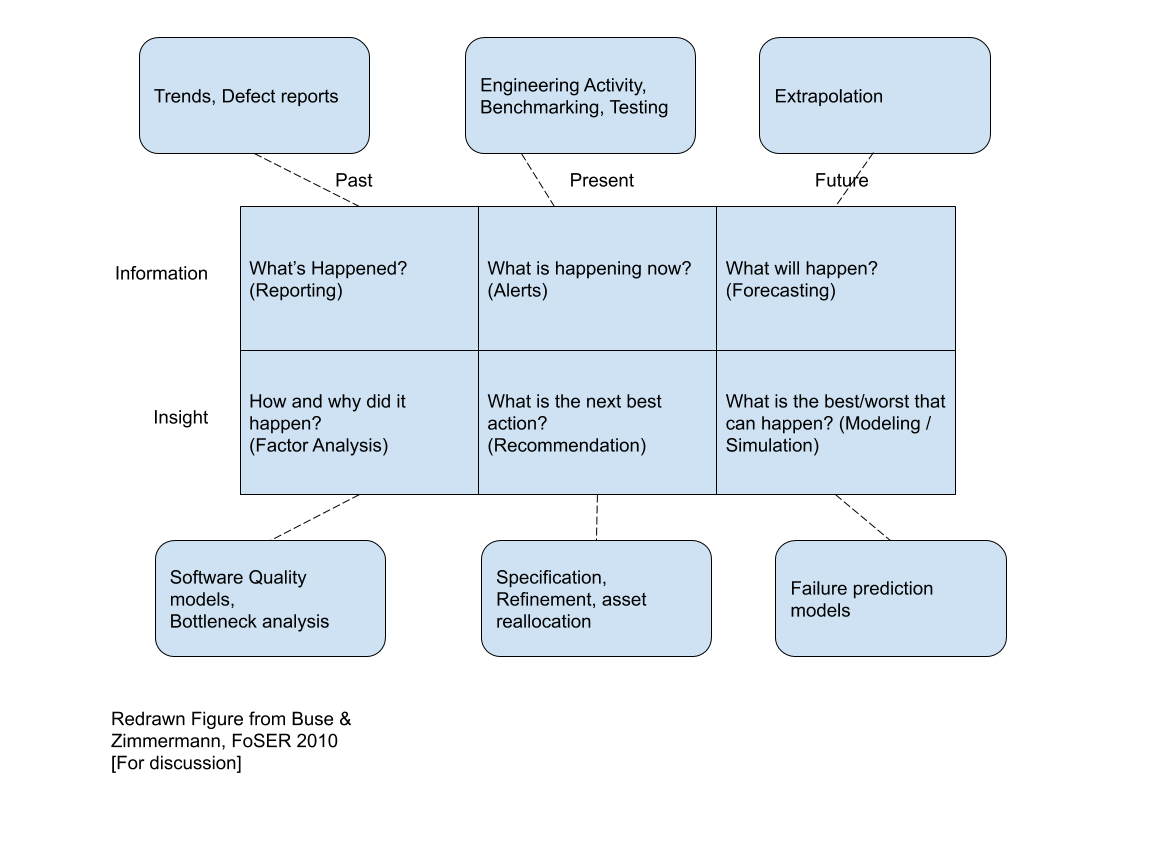
\includegraphics[width=14cm]{images/Buse_and_Zimmermann_2010_figure.png}
    \caption{Software Analytics, Buse and Zimmerman (2010)}
    \label{fig:software_analytics_buse_and_zimmerman_2010}
\end{figure}


In the Buse and Zimmermann paper they \emph{``distinguish between questions of information which can be directly measured, from questions of insight which arise from a careful analytic analysis and provide managers with a basis for action.''}~\cite{buse_analytics_2010}.

\subsubsection{The development managers' perspective}
\emph{``Information needs for software development analytics"}~\cite{buse2012_information_needs_for_software_development_analytics}. They asked 110 Microsofties, a mix of development leads and managers about their use of software development analytics. MUST-DO discuss how my work and their guidelines for software development analytics align. What does my work add to their work? What does it provide that they identified back in 2012? Their focus seems to be more on the code than the product of the code (apps and the services (and the qualities of those services) those apps provide to end users). What information do mobile app developers need in terms of improving the reliability of their apps? How can the developers make good decisions in this area?


\begin{figure}
    \centering
    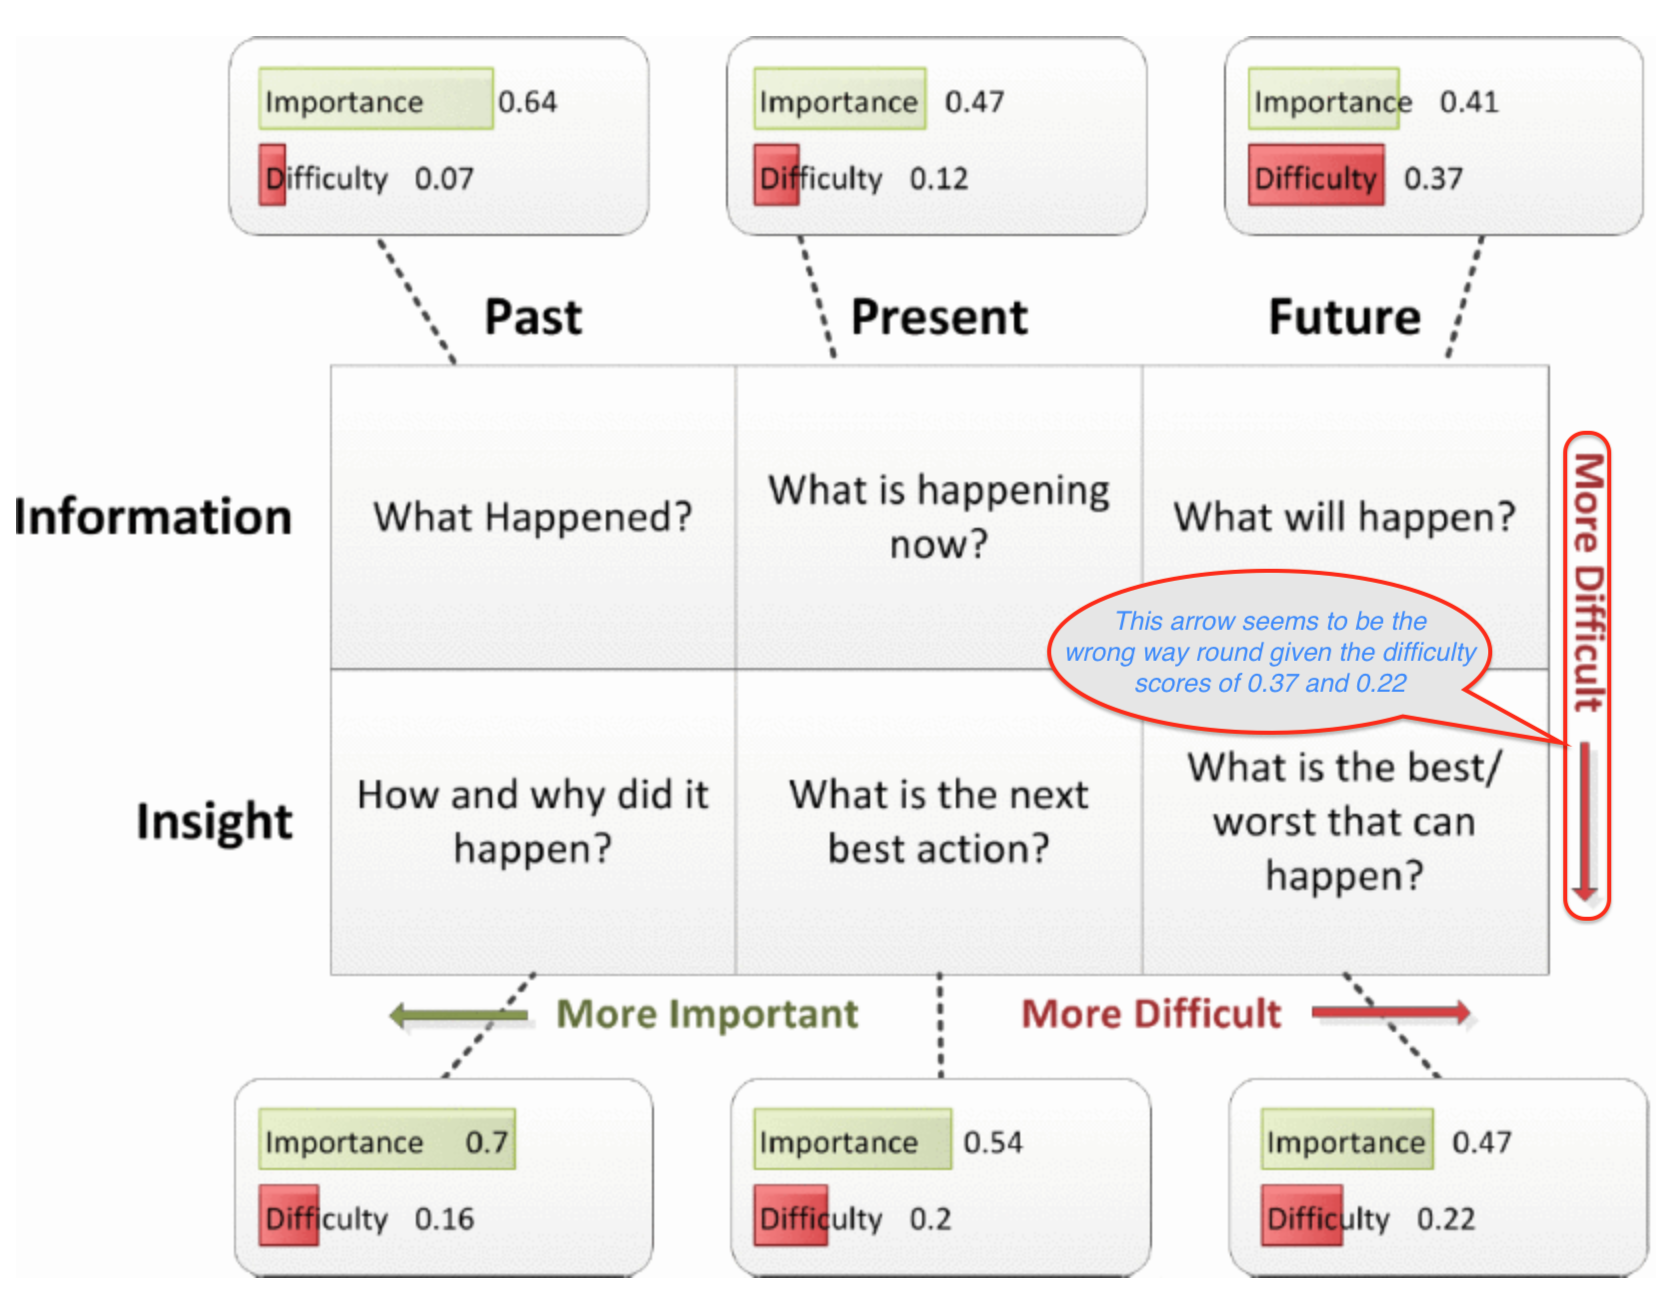
\includegraphics[width=\linewidth]{images/related-work/buse2012-edited-figure-2.png}
    \caption{Revised Figure 2 from TODO}~\footnote{\cite{buse2012_information_needs_for_software_development_analytics}}
    \label{fig:buse2012-edited-figure-2}
\end{figure}


\begin{itemize}
    \item ~\emph{``we ultimately want to} empower software development teams to independently gain and share insight \emph{from their data without relying on a separate entity"}
    \item \emph{``Analytics can help: monitor a project; know what's really working; improve efficiency; manage risk; anticipate changes; evaluate past decisions."}
    
    \item Oddly, Figure 2 in their paper seems to have a mistake in the direction of More Difficult from Information to Insight, see~\ref{fig:buse2012-edited-figure-2}.
    
    \item \emph{``In other words, both developers and managers find it more important to understand the past than try to predict the future; echoing George Santayana, “those who cannot remember the past are condemned to repeat it.”"}.
    
    \item From Figure 4 in their work, Failure Information (\emph{``reports of crashes or other problems"})is in the top 3 that the development leads would use and top for managers when making decisions relevant to their engineering process. Telemetry (\emph{``user benchmarks"} would be used by around 80\% of development leads and 90\% of managers in the survey.
    
    \item \emph{``The landscape of artifacts and indicators in software engineering is well known, but the concrete decisions they might support are not. We conjecture that understanding how managers and developers can make use of information is critical to understanding what information should be delivered to them."}. My research somewhat inverts this by looking at what's being delivered in terms of commercial, pre-existing mobile analytics and considers how that information has been used to improve the reliability of the mobile apps that were the source of the raw information.
    
\end{itemize}~\cite{buse2012_information_needs_for_software_development_analytics}.

\subsubsection{Learning from Windows Error Reporting}~\label{rw-learning-from-wer}
The data collection and analysis of Android Vitals has some similarities with Microsoft's \acrfull{wer}\index{Windows Error Reporting (WER)} which they describe in an article in 2011~\cite{kinshuman2011_debugging_in_the_very_large} and a longer conference paper from 2009~\cite{kinshuman2009_debugging_in_the_very_large}. Similarities include both mechanisms being designed to work effectively at scale of at least a billion end-user machines/devices, capturing crash data, and using error statistics as a tool in debugging. Differences include the platform (Android), the lack of automatic diagnosis (which WER provided), and most relevantly, Google provides several million third-party developers with access to data for the apps they are responsible for and provides them with various comparative analytics of the technical performance of their app compared to those apps of their peers. (Microsoft provided 700 third-party developers, for instance of device drivers, with WER information, and the paper provides a concrete example of how one vendor addressed the top 20 reported issues for their code, and how the fixes percolated out to the end users and halved the percentage of all kernel crashes attributed to that vendor (from 7.6\% to 3.8\%)). Statistics-based debugging, described in these papers, was used in Microsoft's WER and may also apply when developers use mobile analytics.

\subsubsection{Beyond Microsoft}
Microsoft are not unique in publishing research about the use of software analytics. A company, Softeam, used a software analytics platform to collect feedback from their customers and systems with the aim of improving the software quality of their systems~\cite{bagnato2020_challenges_and_benefits_from_using_software_analytics_in_softeam}. They use \url{https://github.com/q-rapids}, a ``Quality-aware rapid software development. H2020 Project (Grant no. 732253)". There are relevant publications listed at \url{https://www.q-rapids.eu/publications}.

\subsubsection{Connecting failures with software analytics}
In a short paper~\sidecite{kidwell2015_toward_fault_taxonomy_application_of_software_analytics}, the authors propose combining fault classification and software analytics for five types of decisions. These are: targetting testing, release planning, judging stability, targeting training, and targeting inspection of software. failure data mined from software analytics tools such as crash reporting tools helps to bring their concepts and ideas to life. Their paper provided initial indicative evidence of their proposals through evaluation of changes to source code for the Eclipse software and discusses the measurement of refactoring to provide more accurate and relevant measurements of the efficacy of the refactoring, rather than considering approaches to improve mobile apps.

\subsubsection{Caveats with software analytics}
% This might be better placed in the discussion or later chapter. TBD.
Using software analytics leads to several \textit{caveats} to consider the `so what' aspects and whether the research is being done well. 
\emph{``Software Analytics, so what?"}~\cite{menzies2013_software_analytics_so_what} to set the context.

\emph{```Bad Smells" in software analytics papers'}~\sidecite{menzies2019_badsmells_in_software_analytics}.

A couple of examples of risks and concerns when using mobile analytics 
\emph{``How Does Misconfiguration of Analytic Services Compromise Mobile Privacy?"} ICSE 2020. This in turn refers to \emph{``Alde: privacy risk analysis of analytics libraries in the android ecosystem."} 2016, and \emph{``Bug Fixes, Improvements, ... and Privacy Leaks - A Longitudinal Study of PII Leaks Across Android App Versions."} 2018.


\section{App Stores and their Effects on Software Development and Engineering}~\label{rw-app-stores-and-their-effects-on-software-development-and-engineering}
% Software developers have flocked to develop mobile apps as that's where billions of users find and use software. In the era of mobile apps before smartphone app stores the device manufacturers and the carriers were the dominant parties. Developers provided their apps directly and/or via carriers and/or a variety of third-party app stores. The ecosystem shortly before the point of inflection is nicely captured in \sidecite{lin2009_os_battle_in_the_ecosystem_of_smartphone_industry}. 

App stores are part of an ecosystem that provides and enforces rules while also constrains various choices while also allowing various freedoms for the participants within the ecosystem. The ecosystem needs to sustain competition~\sidecite[][p. 94]{KAPOOR2021_socio_technical_platform_ecosystems_etc} and revenues. The two largest app stores, Google Play and Apple's App Store, each have their own development platform including an IDE and additional software tools, various SDKs, developer programs, release processes, pricing and revenue rules, and so on. 
%They can effectively severe the connection between developers and their market.
Pivotal effects include: the app approval process (which gates any release of the app to the general user population), rules and restrictions on what the binary contains, the signing process, how the app is packaged/bundled. How app quality is measured and assessed (by the app store, at least - devs have a vested interest in having high quality apps as determined by the app store).

App Stores behave as intermediaries between developers and the users of their software. They make various aspects more transparent including pricing, information about the apps, releases, and ratings \& reviews. There are hundreds of thousands of developers of Android apps according to various sources (320,000 in 2017~\cite{wang2017_exploratory_study_of_the_mobile_app_ecosystem}). 

Many of the developers of the apps are relatively junior, in a detailed survey with 82 respondents~\cite[p. 142 and p.134]{francese2017_mobile_app_development_and_management_results_from_a_quantitative_investigation} Given the youth of the mobile app store concept and the prolific growth of mobile apps from zero to millions in a decade the relative youth of mobile app developers is very plausible and as the paper observes there was a high level of specialization and expertise among the developers surveyed.

In an App Store first the developer then the app store are involved in making a release available to some or all of the user population. There are various competing factors that affect when would be a good time to make a release. Too few and an app may be considered stale or neglected, too many and users may balk at the seemingly endless updates and communications costs. Groups of researchers have investigated various aspects of release engineering, including~\sidecite{adams2016modern} that argues the relevance of modern release engineering and the relevance for researchers, and~\sidecite{nayebi2017version} which concentrates on which version of opensource apps should have been released to the app store. Developers, and their stakeholders, want to make more informed decisions about which releases to make; however there does not appear to have been much research into the testing and quality indicators available to app developers before they make their release public.


This research focuses on the Android ecosystem and the Google Play store - the combination is the preeminent platform in terms of userbase, reach, and platform analytics provided to app developers. Nonetheless, this research also includes research into several additional platforms and app stores, e.g. the Window Phone platform with Microsoft's app store and Huawei's app store for Android, where they contribute to this research. % COULD_DO YY suggests adding a table of the various app stores, I'm holding off doing so as it'd take several hours to compile the supporting information and also I'd then be in a dilemma whether to re-include my material on the Amazon Fire and related app store, etc.


App stores and their ecosystem have affected the lives of billions of end users and millions of software developers. They have become the primary route to market for many app developers and their organisations (exceptions include companies who developed strong businesses elsewhere such as Amazon and Netflix). 
From a research perspective, in 2010, early papers were published on various effects of app stores on academic research e.g. how app stores addressed some of the previous constraints such as reaching more users and facilitating the distribution of the apps and feedback from those users. 

Cramer \emph{et al} discussed aspects of \emph{research in the large} and in particular for my research the importance of ``playing by the rules"~\sidecite{cramer2010_research_in_the_large_app_stores}. This research identified the importance of what happens when developers were deemed not to play by the rules (covered in \secref{rw-power-dynamics-topic}) and this research has been shaped to play by the rules of the app store. % Where practical through responsible disclosure of flaws found in 

Miluzzo \emph{et al} introduced other relevant research aspects, \textit{i.e.}  ongoing concerns such as how to assess correctness when there is no \emph{``ground truth"} - a challenge when evaluating mobile analytics for shipping apps; and a software development model of \textit{``deploy-use-refine"}~\sidecite{miluzzo2010research_in_the_app_store_era}, where app development refines the app based on data gleaned from usage of the app. Their paper even explained how a silly mistake caused their app to crash where the app store then delayed the new release of the app by several weeks. Even in 2010 crashes adversely affected the app store's perception of an app.\todo{TBD where should I mention that our case studies used usage data to refine the app to improve the measured reliability of the apps.} % Their work on CenseMe received an ACM Test of Time award, see https://www.cs.dartmouth.edu/~campbell/page-3/


In more recent research, \textcite{wang2019_understanding_the_evolution_of_mobile_app_ecosystems_a_longitudinal_measurement_of_google_play} provided an helpful longitudinal evaluation of the Google Play ecosystem and raises interesting questions and observations about Google Play; but does not seem to consider flaws, or the effects of flaws, in the app store's data collection, algorithms,\textit{ etc.}

In terms of effects of app stores on software engineering practices there have been several seminal papers written by authors at UCL as part of their App Store Analysis Group~\footnote{http://www0.cs.ucl.ac.uk/staff/F.Sarro/projects/UCLappA/UCLappA.html} while it was active (until roughly 2019). Of these papers, \emph{``App store effects on software engineering practices"}~\sidecite{alsubaihin2019app_store_effects_on_software_engineering} combined interviews with a survey to ask developers of their experiences of developing mobile apps and how those experiences differed with developing other software. There are plenty of other papers that consider the app store from various perspectives but they do not cover software quality or mobile analytics.

Of the ten developers they interviewed a couple were for popular apps (800,000 downloads, 2,000 ratings, 1,000 ratings), the rest were for less popular apps. % 0.1% ratings to downloads for a developer of 1M downloads app: https://www.quora.com/What-is-a-typical-ratio-of-reviews-to-active-users-to-downloads-for-iOS-and-Google-Play-apps
Their research identified automatic in-app crash reporting as the most frequent source of bug reports and the second-most frequently addressed in terms of bug fixes (end-user written bugs were addressed slightly more frequently)~\cite[p. 10]{alsubaihin2019app_store_effects_on_software_engineering}. 

Of particular interest was the discovery that the quality of the [source] code was the least important factor to build a successful app according to the survey results and furthermore the number of downloads were the highest measure of success~\cite[p. 13]{alsubaihin2019app_store_effects_on_software_engineering}\todo{Replace repeated citations with \emph{ibid}?}. Note: Google subsequently (but not necessarily because of this research) have placed a lot of focus on encouraging developers to improve the quality of their Android apps in Google Play. 

Their research is one of several that discusses the gaming of app store ratings, such gaming is unsurprising given the importance placed on these ratings and particularly in having mobile apps with high ratings in the app store. Ratings and reviews are one of the topics of the next section \secref{rw-sources-of-info-on-software-quality-for-devs-of-mobile-apps} given their importance in the mobile app ecosystem.

\emph{Future Trends in Software Engineering Research for Mobile Apps}~\sidecite{nagappan2016_future_trends_in_sw_eng_for_mobile_apps} focuses attention on the software development life-cycle, it does not investigate usage or operational aspects. Figure~\ref{fig:nagappan2016_future_trends_in_sw_eng_for_mobile_apps_figure_1_annotated} is an annotated version of their Fig. 1. [on p. 22](\textit{ibid}) where the annotation shows the key operational and usage areas this work did \emph{not} cover. 


% Note this could do with expanding while retaining the citation (which leads to Float(s) lost quite often) I'd prefer the proper begin{figure) that's currently commented out.
    {\centering
    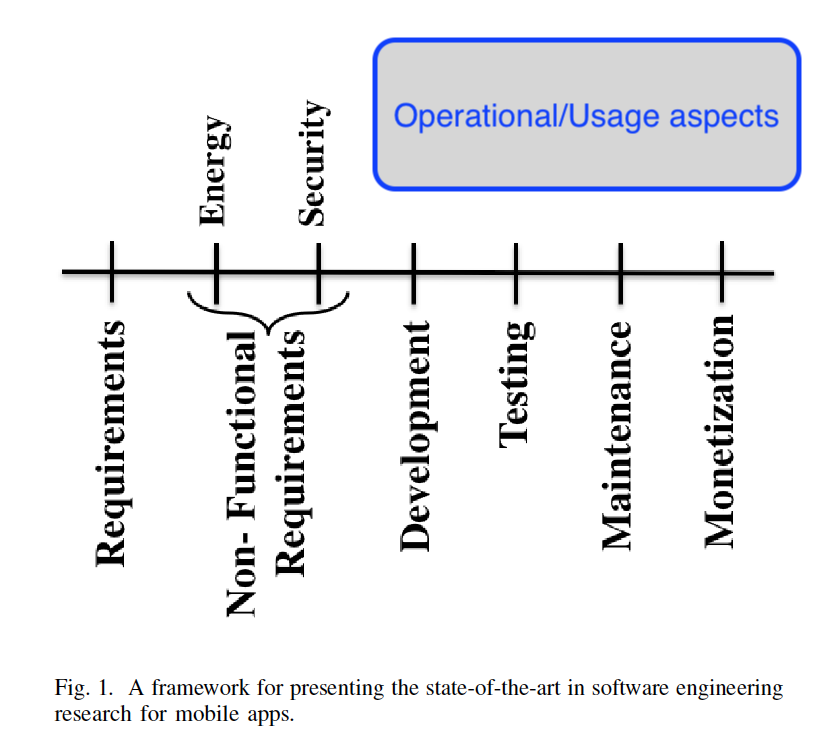
\includegraphics[width=\linewidth]{images/related-work/future-trends-in-sweng-for-mobile-apps-fig-1-annotated.png}
    \captionof{figure}{Annotated version of the framework for presenting the state-of-the-art in software engineering for mobile apps~\cite{nagappan2016_future_trends_in_sw_eng_for_mobile_apps}}
    \label{fig:nagappan2016_future_trends_in_sw_eng_for_mobile_apps_figure_1_annotated}
    } % Thanks to https://tex.stackexchange.com/a/232290/88466

\begin{comment}

\begin{figure}
    \centering
    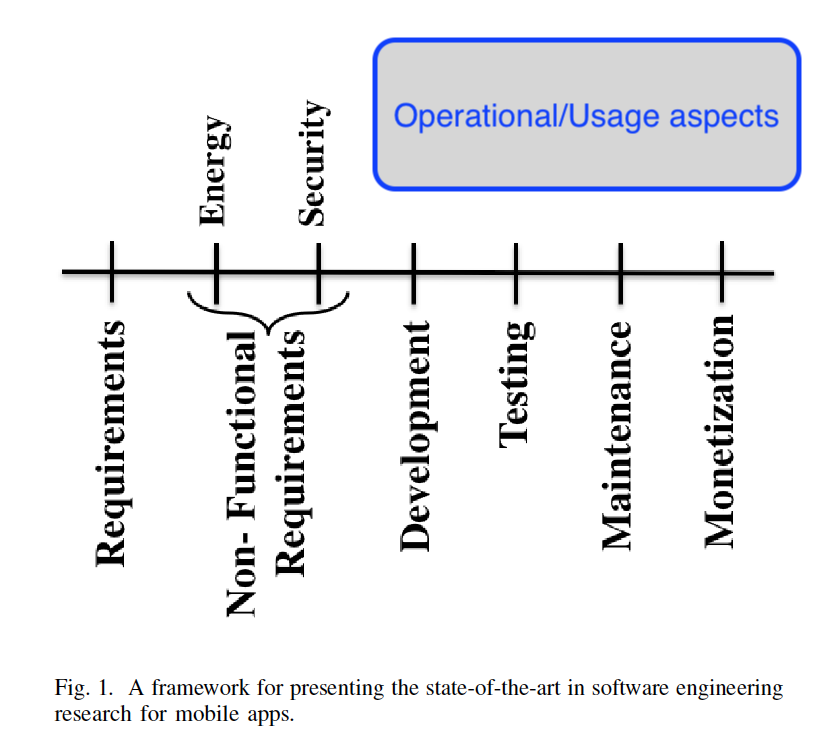
\includegraphics[width=\linewidth]{images/related-work/future-trends-in-sweng-for-mobile-apps-fig-1-annotated.png}
    \caption{Annotated version of the framework for presenting the state-of-the-art in software engineering for mobile apps~\cite{nagappan2016_future_trends_in_sw_eng_for_mobile_apps}}
    \label{fig:nagappan2016_future_trends_in_sw_eng_for_mobile_apps_figure_1_annotated}
\end{figure}
\end{comment}

Mining review data for various forms of data including requests for bug fixes as is using rating as an assessment of goodness. 
Figure~\ref{fig:nagappan2016_future_trends_in_sw_eng_for_mobile_apps_figure_2_annotated} is an annotated version of their Fig. 2 [on p. 23](\textit{ibid}). The annotations include feedback in the forms of ratings and reviews and in the form of mobile analytics. Various sources of information can be used by the development team, of these ratings and reviews are broadly researched, whereas device-level and app-level analytics have not been previously researched.


% Note this could do with expanding while retaining the citation (which leads to Float(s) lost quite often) I'd prefer the proper begin{figure) that's currently commented out.
    {\centering
    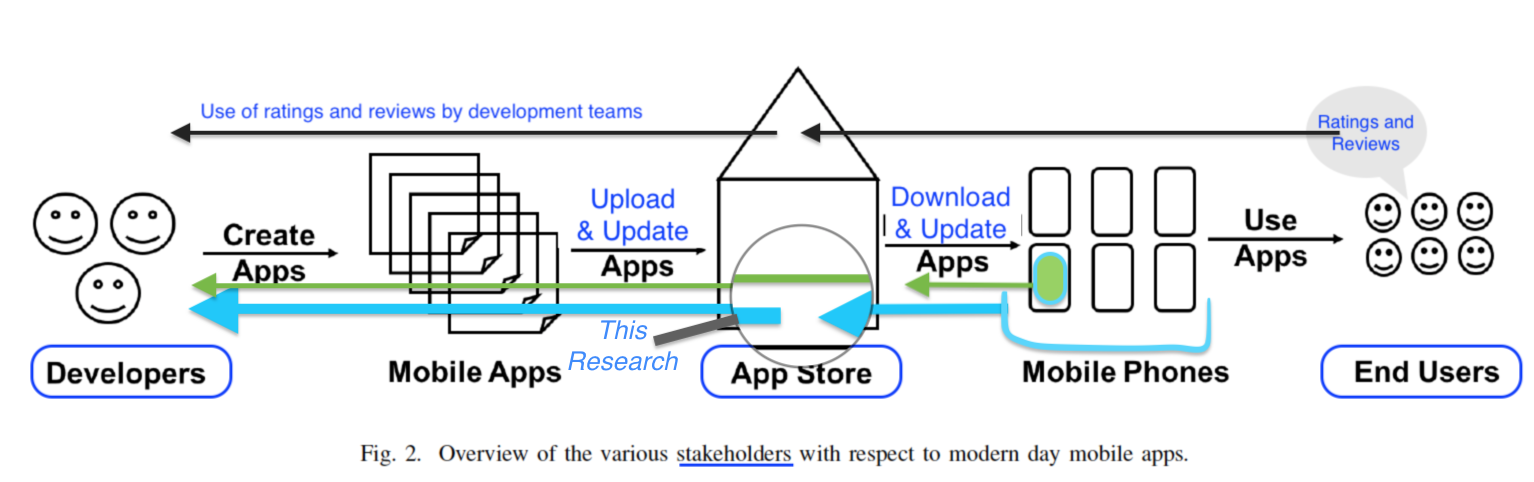
\includegraphics[width=\linewidth]{images/related-work/future-trends-in-sweng-for-mobile-apps-fig-2-annotated-with-highlights.png}
    \captionof{figure}{Annotated version of the various stakeholders in the modern app store ecosystem~\cite{nagappan2016_future_trends_in_sw_eng_for_mobile_apps}}
    \label{fig:nagappan2016_future_trends_in_sw_eng_for_mobile_apps_figure_2_annotated}
    }
  
\begin{comment}
\begin{figure*}
    \centering
    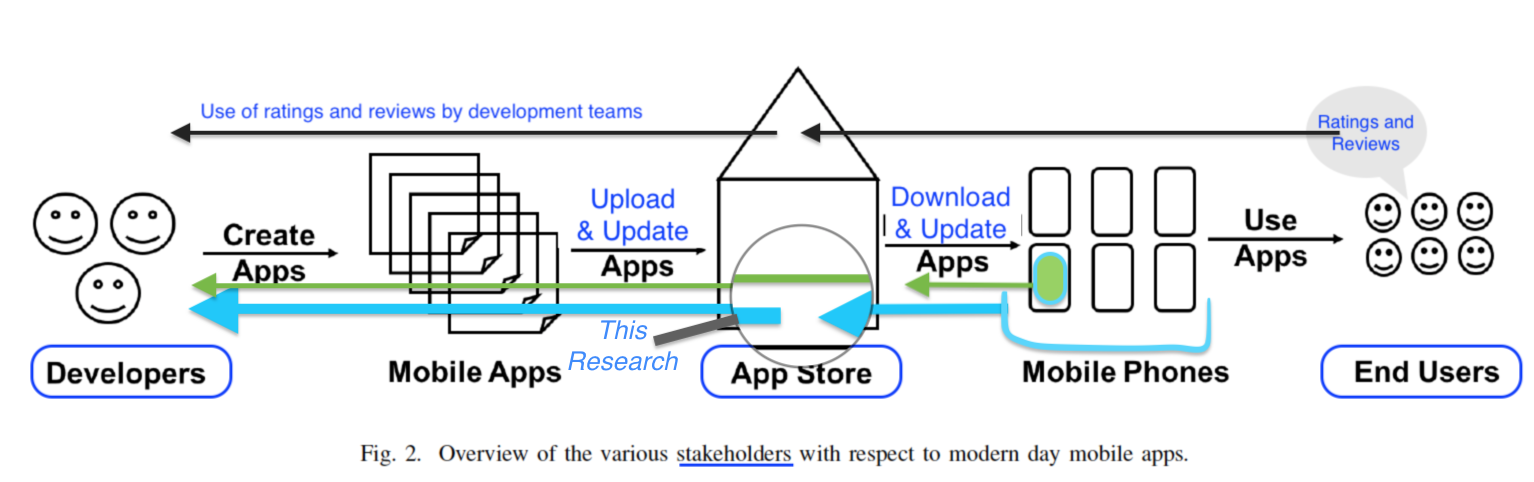
\includegraphics[width=\linewidth]{images/related-work/future-trends-in-sweng-for-mobile-apps-fig-2-annotated-with-highlights.png}
    \caption{Annotated version of the various stakeholders in the modern app store ecosystem~\cite{nagappan2016_future_trends_in_sw_eng_for_mobile_apps}}
    \label{fig:nagappan2016_future_trends_in_sw_eng_for_mobile_apps_figure_2_annotated}
\end{figure*}
\end{comment}  

One of the key challenges identified is restricted access to data held by the app store. The only way they mentioned was to gather historical information by continually mining the app store on a regular basis, [pp 22-23](\textit{ibid}). Perhaps the authors weren't aware that developers of Android apps have access to various historical data about their apps including long term access to all the reviews of their apps. Details of how developers can download these and other reports, including the data structures, are available online~\sidecite{google_play_download_and_export_monthly_reports}.

An area their work did not discuss is whether failure data could, potentially, be a form of requirements? (in a similar fashion to leveraging reviews in the app store to extract `requirements'). And similarly can complaints and failure data be combined to help developers prioritise issues they should consider addressing (the paper restricted the discussion to prioritising issues the developers should be \textit{testing} for).

Finally in terms of this paper, they included two stakeholders, the developers and the end users. The app store (and the people and organisation who provide the app store) are also direct stakeholders in the ecosystem. There are additional indirect stakeholders including advertisers, researchers, and probably many others. 

\subsection{Utility and Service Providers}~\label{rw-utility-and-service-providers-topic}
Developers use software and related services from various providers where the providers are the primary source of any updates. The providers may charge for their offerings and similarly they may mandate various behaviours from developers and their organisations who use the utilities and/or services.

In the context of this research mobile analytics are provided as utilities and/or services by third-parties to app developers therefore it is useful to learn of pertinent research into the use of these utilities and services. Utilities include software tools, libraries, frameworks, and so on; and services may be provided either for some of these utilities or for additional capabilities, support, and so on. Some of the offerings are specific to mobile apps, however many include other platforms such as web sites and/or web apps. Of these examples, an understanding of the use of software libraries helps identify the proclivity of developers to use them and similarly services that apps use are particularly relevant.


\newthought{Libraries: }
Developers can choose to use external libraries to generate revenue (ads)~\sidecite[][p. 407]{li2016_an_investigation_into_the_use_of_common_libraries_in_android_apps}, to \emph{ease the management of HTTP requests}~\sidecite[][p. 73]{belkhir2019_an_observational_study_on_the_state_of_rest_api_uses_in_android_apps} and in their related work they found 98\% of android apps used third-party libraries in their apps~\sidecite[][p. 218]{abdellatif2020_a_multi_dimensional_study_on_the_state_of_practice_of_rest_apis_usage_in_android_app} and on average 41\% of android apps is contributed by common libraries~\sidecite[][p. 409]{li2016_an_investigation_into_the_use_of_common_libraries_in_android_apps}. Using the data in Fig. 5 of this paper (on p. 409) 5\% of the apps included Google Analytics and 2.6\% used Flurry analytics. Note: Industry data indicates mobile analytics are now incorporated in the vast majority of Android apps.  

\newthought{Services: }
Two of the extremely popular categories of third-party libraries are advertising (ads) and mobile analytics.\todo{add examples from research using appbrain examples as a grey data backup/alternative.}
In some ways app developers appear to be similar to their end-users - neither wants to pay up front for what they use.\todo{Add research into the ratio of free to paid apps.} Typically service providers have at least one form of unpaid service offering either time or volume based, many then also have at least one paid-for service offering that do not have the same restrictions of their unpaid offering.

Remote device farms are good examples of services that at least some developers (and/or their organisations) pay for. A relatively dated paper about the then current device farm services provides a useful overview~\sidecite[][]{starov2015_taas_for_mobile_apps_survey} but does not discuss pricing and it predates the now popular service offerings by Google, Amazon, and others. I'm not aware of much research into the use of these device farms apart from some in Brazil IIRC who used an opensource backed test lab service. 

\subsection{Using app store crash analytics to automatically find robustness and reliability failures}~\label{rw-windows-phone-store-crash-analysis-section}
There was a breakthrough stream of work and research that was developed for Microsoft's now defunct mobile app store for Windows Phone devices. That work included mining 25 million crashes~\footnote{Note: The 25 million crashes were a small subset of the total crashes on end-user devices were a subset of the total based on their third footnote ``The developer has no control over the probability.''~\cite[p. 191]{ravindrath2014_automatic_and_scalable_fault_detection_for_mobile_apps}.} that occurred in 2012 on end-user devices when using various apps on their Windows Phones~\cite[p. 190]{ravindrath2014_automatic_and_scalable_fault_detection_for_mobile_apps}. They determined the top 10\% of error buckets covered more than 90\% of crashes~\cite[p. 192]{ravindrath2014_automatic_and_scalable_fault_detection_for_mobile_apps} and discovered a significant proportion of these stemmed from root causes they could generate externally. For example, they could configure a network proxy to return a HTTP 404 response to a network request for network calls made by any of the mobile apps [p. 192].

They built a service called VanarSena to run in the cloud on lots of Windows Phone emulators with the purpose of automatically testing Windows Phone apps. The service automatically instrumented these apps, for instance to add a global Exception handler (the complete set of five injected modules are described in pp. 193..194). The app is exercised using autonomous automated testing tools called~\textit{monkeys} and the service includes a range of fault inducing modules (FIM) [p. 196] that provide inputs and conditions including those that have caused existing apps to crash. 

This paper includes lots of additional practical information that would be pertinent for providers of similar services \emph{e.g.} for other automated testing providers and/or app store providers which we can skip here as they are not closely related to using mobile analytics. Instead, let's concentrate on key characteristics of their work:

\begin{itemize}
    \item Their work built on earlier work of some of the authors where that work was performed at a smaller scale on Android~\cite{ravindrath2012_appinsight_mobile_app_performance_in_the_wild}. They share a common instrumentation framework implemented first for Android then for Windows Phone.
    \item The authors proposed VanarSena could be provided by an app store to help test new releases before they were released in production. The automatic testing helps establish whether the apps handle non-ideal conditions without crashing.
    They describe crash buckets and a) identified commonalities in those crash buckets, b) found a significant subset could be triggered through manipulating inputs, conditions, and responses to the app.
    \item The results of their research included finding 1108/3000 production Windows Phone apps had failures that were detected by VanarSena. They uncovered 2969 distinct bugs in these apps including 1227 that were not previously reported~\cite[p. 202]{ravindrath2014_automatic_and_scalable_fault_detection_for_mobile_apps}. Some of the failing apps had been developed by professionals others by amateurs - this indicates developers often write code that does not cope adequately with non-ideal circumstances.  
\end{itemize}

Several of the authors of the previous paper collaborated with other colleagues at Microsoft Research to extend the work. In ~\textcite{chandra2015_how_to_smash_the_next_billion_mobile_app_bugs} they describe various improvements to their Caiipa service that delivered eleven-fold more crashes and eight-fold more performance problems~\cite[pp. 37-38]{chandra2015_how_to_smash_the_next_billion_mobile_app_bugs}. The core of their paper presents their plans for a sophisticated automated testing system for testing Windows Phone apps together with their goals and challenges. The most pertinent goal in terms of this research would be actionable reports~\cite[p. 36]{chandra2015_how_to_smash_the_next_billion_mobile_app_bugs} together with their use of context data and historical data. 

Given the nature of Microsoft's objectives they did not consider Mobile Analytics or crash reporting SDKs (which include breadcrumbs and the ability to report caught errors, \emph{etc.}). Nor do their papers mention how the app developer's perceived their various tools and services. It's unclear whether they actually involved app developers in their work. Also, given the demise of the Windows Phone platform and app store it appears much of this work has disappeared without a trace.


\subsection{Power dynamics}~\label{rw-power-dynamics-topic}
Grey literature is the main source of the imbalance in power between app developers and the app store, at least in terms of Google Play and Android apps in that store. I have selected four illustrative articles, by four different developers, of the 20+ related articles published on \href{https://medium.com/}{Medium} % More material is available on corporations on mining data from the public  from and via https://jilliancyork.com/
about how they lost access to their apps and in some cases their account. 

In \textcite{martinez2019_google_just_terminated_our_startup_google_play_publisher_account_on_xmas_day} the termination of a personal Google Play account for an indirectly associated developer, via one of the employees of the small company, was attributed to the termination of that company's Google Play account. This story has ongoing updates that lists various developers who have had similar experiences. A similar experience was reported by \textcite{dodson2019_google_completely_terminated_our_new_business_etc} where apparently someone's associated account was the cause of Dodson's account being terminated. As Méa dry noted \emph{``google@play-store: sudo rm -rf org.mtransit.android*''} which happened abruptly within a few hours of sending an email notification to the developer. The reason given in the automated emails was the app was in violation of the ``Deceptive Behavior policy''~\sidecite{mea2019_google_just_deleted_my_nearly_10_year_old_app_etc}. 

In these three instances the developer accounts were reinstated. In \textcite{marcher2021_how_google_terminated-a-developer} the account was not reinstanted and two of his clients also had their accounts terminated. As Marcher notes \emph{``I develop software not just for fun but also primarily for a living. This action not only deprives me of a substantial part of income, but it also forbids me for life to continue my work which is also my passion''}. % See also https://medium.com/@appsrentables1/google-cancels-our-google-play-publisher-account-and-ends-my-familys-source-of-income-97d4e85cd046 and various others (20+ stories)

\subsection{Developers and their app counts}
Before we leave the topic of App Store ecosystems and in particular a developer focused perspective on the ecosystem, the work of \textcite{wang2017_exploratory_study_of_the_mobile_app_ecosystem} looks potentially interesting as it states it looked at the Google Play store from a developer's perspective; the title appears misleading as they actually researched mappings between developers and the number of apps they had in Google Play Store. In other words, the paper concentrates on the characteristics of developers who have many apps in the app store rather than on the software development/engineering aspects.

They estimated there were 320,000 developers, over half of the developers only released a single app. The paper main focus though is on the \emph{``the group of aggressive developers who have released more than 50 apps, trying to understand how and why they create so many apps''}. In terms of this research this paper provides some context on who writes the mobile apps in Google Play, provides an estimate of the population of developers (in 2017).


\section{Developing Mobile Apps}~\label{rw-developing-mobile-apps-section}
Research into the development practices and mechanisms for mobile apps establishes various norms, characteristics, and habits, of app developers. Their work, collectively, is used by billions of people throughout the world. In terms of this research, understanding the development practices and mechanisms is vital. Developers also have a voice and hundreds have been interviewed to learn what's important to them, for example in \sidecite{joorabchi2013_real_challenges_in_mobile_app_development}. They also communicate through various artefacts they create and maintain, again these artefacts have been studied to learn about their work, for example in \sidecite{pascarella2018_self_reported_activities_of_android_developers}.

% Some of the effects of their work in terms of software quality will be covered later in this chapter in \secref{rw-mobile-app-crashes-topic}.

Mobile apps need to be made and developers make them. There are various working practices, apps are made by visionaries, employees, amateurs, and communities. There are various activities involved including development, testing, release, and deployment. % Figure~\ref{fig:my_mobile-app-makers} highlights these activities as part of the overall ecosystem.

% Many mobile app development teams would describe their development practices as Agile or based on along the principles of Agile development. % Solo app developers are less likely to use these practices, nonetheless there has been various research into adaptions of Agile and Scrum in attempts to suit them. Various examples are in the excluded-bibliography.
% Many of these people claim to be ``Agile" in their working practices.

5,000 commit messages (of over 1.8 million identified) were studied that were selected from 8,280 active opensource Android apps where the source code repositories were on github.com. The top three activities were 1) app enhancement, followed by 2) bug fixes, and then 3) project management~\sidecite[][p. 144]{pascarella2018_self_reported_activities_of_android_developers}. 35 of the commit messages were attributed to addressing crashes in the app [Figure 3, on p. 151]. They did not investigate how developers had discovered issues nor whether mobile analytics were affected in the commits, leaving these aspects unknown and unreported.

Relatively early research, published in 2013, identified several key topics of concern for app developers including: a strong need for monitoring and analysis support, for instance to monitor the health of an app. Similarly a major problem was crashes \emph{``which are often intermittent, non-deterministic, and irrecoverable.''}~\sidecite[][p. 21]{joorabchi2013_real_challenges_in_mobile_app_development}. Interestingly, one of the discussion topics was to research testing \acrshort{api}s from App Stores[pp. 22-23] which predates Google Play's Pre-launch reports covered in \secref{tata-pre-launch-reports-topic}.


As mentioned previously, in \secref{rw-utility-and-service-providers-topic}, Android apps incorporate software libraries extensively~\sidecite{li2016_an_investigation_into_the_use_of_common_libraries_in_android_apps}. The extensive use of software libraries, generally provided by third-parties, indicate the developers place significant trust with these third-party developers. Also, their apps contain large volumes of code that is \emph{unlikely} to have been tested by the app developers apart from some sanity and/or smoke testing. Flaws and instabilities in these libraries may be latent until the app is being used at scale by end users. How will the developers learn about the effects of emergent flaws and instabilities?

Note: in terms of trying to understand real-world practices please avoid \textcite{santos2016_investigating_the_adoption_of_agile_practices_by_20_undergrad_students_in_mobile_app_devt} which sounds relevant but only surveyed 20 undergraduate students who took an iOS development course. 

\subsection{Testing Mobile Apps}~\label{rw-testing-mobile-apps-topic}

There has been a tremendous amount of research into practices and tools that might perform better than the mainstream test automation tools available to app developers.

A useful categorisation of testing for mobile apps may be: 
explicitly designed scripted tests, 
automatic robots that navigate and sometimes interrogate target apps, and 
hands-on testing which often vary depending on who performs them and each instance of the testing. 
Where the testing may be performed:
on local physical devices,
on remote physical devices in the `cloud'
on local emulators and/or local simulators, and
on remote emulators and/or simulators.


There has been a lot of research into various artefacts pertaining to mobile apps. Some of the artefacts are mainly generated by end users, for instance ratings and reviews, and others are mainly generated by software developers such as source code. A hybrid artefact are bug reports. These also known as issues particularly for projects based on github.com as it uses that term and developers create bug reports as issues on github.com. Bug reports are a hybrid artefact as potentially anyone can create them including users of the code and the development team. 

That said, for the projects studied in this research they mainly used `issues' and these were mainly created by the project's extended development team (an extended development team may include people involved in project management and/or testing).

\subsubsection{Papers to consider}
\begin{itemize}
    \item Discuss the TestDroid paper! it describes testing that was actually done by developers!~\cite{kaasila2012_testdroid_etc}.
    
    \item \emph{``Is Mutation Analysis Effective at Testing Android Apps?"}~\cite{deng2017_is_mutation_analysis_effective_at_testing_android_apps}.
    
    \item \emph{``Mining Android Crash Fixes in the Absence of Issue- and Change-Tracking Systems"}~\cite{kong2019_mining_android_crash_fixes}.
    
    \item \emph{``How do Developers Test Android Applications?"}~\cite{linares2017_how_do_developers_test_android_apps}. Quote:~\emph{``“I mostly do manual testing due to the limited size of my apps. I sometimes use a custom replay system (built into the app) to duplicate bugs after I come across them. This method is usually combined with manual testing (printing debug information to the log) to pinpoint the cause”."}
    
    \item \emph{``First Steps in Retrofitting a Versatile Software Testing Infrastructure to Android"}~\cite{oliver2018_first_steps_in_retrofitting_a_versatile_sw_testing_architecture}.
    
    \item \emph{``A Large-Scale Study of Application Incompatibilities in Android"}~\cite{cai2019_large_scale_study_of_android_incompatibilities} An oddly insipid paper which promised some interesting run-time issues discovered in their research where the Android version would be a likely cause. However the reproduction package lacked the test scripts or means to reproduce their testing or bug detection. Also, their research now seems to be less relevant in 2020 as Android apparently improved the backwards compatibility \emph{``Yet newer versions (since API 24) had no run-time compatibility issues with apps created in the studied span."}. Their work may well have merit for the research community, It does not appear to have much relevance to developers of real-world Android apps today.
    

    \item \emph{``Intent Fuzzer: Crafting Intents of Death"}~\cite{10.1145/2632168.2632169} TODO Link this to the industrial case study and the Kotlin NPE crash.
    
    \item \emph{``Linares-Vasquez et al. [56] propose MonkeyLab, which mines recorded executions to guide the testing of Android mobile apps."} Their approach records GUI events (click events). Members of the project team (developers, testers, etc.) perform the actions, the authors claim their log collection process could scale to collecting logs from ordinary users. Key limitations include events that aren't purely dependent on the user's GUI inputs, there would also be challenges getting users to accept such an approach where the app records every input they made. Also, they generate GUI events that have x,y coordinates - absolute positioning that may have limited portability to other devices, screen rotations, and so on. Their playback also appears to require rooted devices. There are numerous other limitations described in their paper, nonetheless their work shows promise in terms of detecting and generating patterns the students did not find. It would be interesting to compare the results using accomplished software testers with experience and expertise testing similar Android apps.
    
    \item \emph{``An Empirical Study of Android Test Generation Tools in Industrial Cases''}~\cite{wang2018_an_empirical_study_of_android_test_generation_tools_in_industrial_cases} 
\end{itemize}

There has been a tremendous and sustained research interest in software testing, for instance testing is one of the most popular topics at the ICSE series of conferences~\footnote{\url{https://dl.acm.org/conference/icse}} and the focus of entire conferences including AST~\footnote{\url{https://conf.researchr.org/home/icse-2020/ast-2020}}, ICST~\footnote{\url{https://conf.researchr.org/series/icst}}, and so on. Similarly the application of software testing to mobile apps is a rich topic with sustained interest in the challenges and facets of testing mobile apps.

The facets include automated testing and automated bug reproduction, maximising the `bang for the buck' for instance in selecting which device models would be most valuable to use with finite testing. Understandably given the field where many of the authors work - in research - the vast majority of the research is on software apps they have access to, software their can obtain the source code for (particularly opensource), software they can write, and the people they have available to them (other researchers, students, voluntary participants, and people paid to paid to perform specific tasks). Minute amounts of the work is based on mature, popular software with semi- or fully- professional developers and development teams. Some research projects, particularly CRASHSCOPE~\cite{moran2016_automatically_drr_android_app_crashes}, offer the potential to reproduce some of the crashes reported by Mobile Analytics if the tools are sufficiently available and current to actually use.




\subsubsection{Prioritising devices to test on}

Selection criteria include:
\begin{itemize}
    \item the relative popularity of a single app across the user base for the app, provided by OpenSignal, and reported over a three year period,
    \item the usage of similar, popular, Android apps for two app categories: grouped by device model as measured by a very popular app management app in China,
    \item the devices used most frequently by users who write reviews for the same Android app,
\end{itemize}

One of the research papers close to the area of my research uses usage data for two popular app categories (games and media) gathered through a popular Android management app in China~\cite{lu2016_PRADA}. Their work uses an operational profile to prioritise the device models to select to test both new or existing apps. The management app, called Wandoujia~\footnote{\url{https://www.wandoujia.com/}}, is used by \emph{`500 million people to find apps they want`}~\footnote{According to Chrome Browser's automatic translation from Chinese.}. Daily usage of the top 100 apps in the two app categories was collected for various device models. In various ways the Wandoujia app management app provides similar capabilities to Google Play, including tracking when apps are installed, and in use. The recommendations are coarse-grained. The research measured the accuracy of their predictions for recommended devices with the actual devices that the app ended up being used on once the app had been launched. 

Their work demonstrates that usage data for several app categories was useful to guide developers on the most popular actual device models for their app. They acknowledge several limitations in their work, including their use of incomplete measures such as foreground network activity for usage which don't suit apps that either perform network processing in the background or don't use the network. Other app management services, particularly Google Play, could provide similar guidance to app developers. And indeed as Google Play collects additional data for the entire apps store it could cover some of the gaps and limitations identified in this research.


\subsubsection{Device Testing Services}
Test Farms have been available commercially since around 2008~\footnote{Based on the author's professional experience.}. Over the years different offerings have peaked and then either been acquired, retired, or disappeared. Google, Amazon and Microsoft offer paid-for device farms as do various specialist businesses. There have been a couple of public-good initiatives including Open Device Labs~\footnote{For example~\url{https://opendevicelab.com/},~\url{https://www.devicelab.org/}}; and Open STF~\sidecite{openstf_website} which is based on a set of opensource projects~\url{https://github.com/openstf/} and enables teams and organisations to build their own device farms or use commercial offerings based on these projects~\footnote{For example~\url{https://www.headspin.io/}.}.
% https://loadfocus.com/blog/tech/2018/04/building-your-in-house-device-farm-on-mac-os-using-openstf-for-android-testing/ 
% https://tech.mercari.com/entry/2019/02/18/173236 (on using HeadSpin and NimbleDroid).



\subsection{Maintenance of mobile apps}

\emph{``The area of software maintenance is one of the most researched areas in Software Engineering. However, due to the fact that mobile apps is a young subarea within SE, the maintenance of mobile applications remains to be largely undiscovered."}~\cite[p. 27]{nagappan2016_future_trends_in_sw_eng_for_mobile_apps} - My work does investigate aspects of maintenance. 

\emph{``Syer et al. [93] compares mobile apps to larger “traditional” software systems in terms of size and time to fix defects. They find that mobile apps resemble Unix utilities, i.e., they tend to be small and developed by small groups. They also find that mobile apps tend to respond to reported defects quickly."}~\cite[p. 27]{nagappan2016_future_trends_in_sw_eng_for_mobile_apps} - Check the details of what quickly means and how the teams discovered the defects.

\emph{``Bavota et al. [16], show that the quality (in terms of change and fault-proneness) of the APIs used by Android apps negatively impacts their success, in terms of user ratings. Similarly, McDonnell et al. [65], study the stability and adoption rates for the APIs in the Android ecosystem."}~\cite[p. 27]{nagappan2016_future_trends_in_sw_eng_for_mobile_apps} - Skim read both these papers to determine their relevance.

\emph{``Another line of work examined Android-related bug reports. Bhattacharya et al. [18] study 24 mobile Android apps in order to understand the bug-fixing process. They find that mobile bug reports are of high quality, especially for security related bugs. Martie et al. [63] analyzed topics in the Android platform bugs in order to uncover the most debated topics over time. Similarly, Liu et al. [58] detected and characterized performance bugs among Android apps."}~\cite[p. 27]{nagappan2016_future_trends_in_sw_eng_for_mobile_apps} - Looks at how the bugs were fixed and compare the practices they detected with those I'm aware of. Are platform bugs that relevant? They look at performance bugs (Android Vitals also reports performance issues, Firebase Analytics has tools for performance tracking), I'm looking mainly into reliability measurements and issues.

Following on from the challenges and future directions section on maintenance research for mobile apps: do researchers focus in areas where the streetlights are rather than where the problems are? \emph{i.e.} on where they can find material to study rather than on issues that practically affect the majority of developers of apps?

\emph{``Charting the API minefield using software telemetry data"}~\cite{Kechagia2015_charting_API_minefield_using_telemetry_data}. The stability of Android apps has been measured using telemetry data collected by a centralised crash report management service. Roughly one million stack traces were analysed from thousands of Android applications. A subset (over 500,000) of these stack traces were associated with risky API calls and these were analysed to identify the most common failure reasons. The top five reasons were attributed to:
    \begin{itemize}
        \item memory exhaustion,
        \item race conditions,
        \item deadlocks,
        \item missing resources, and
        \item corrupt resources.
    \end{itemize}
    
    The authors provide a set of recommendations they claim \emph{may} help address various classes of the crash failures. However these recommendations do not appear to have been tested for their efficacy. Their recommendations are theoretical rather than practical. There's an odd claim in the paper in page 1818, \emph{``In addition, the platform of Chen et al. (2011), which is based on remote resource management, can make applications require less memory and resources. Hence, it can eliminate the well-known “non-responsive” exceptions in Android."}. For this claim to hold true \textbf{all} the causes of non-responsive exceptions (or did the authors mean ANRs? they don't define this term or use it elsewhere in the paper) would need to be a) related to remote resources, and b) the difference would need to be directly related to the amount of memory and resources. Google provides five common patterns for diagnosing ANRs~\footnote{\url{https://developer.android.com/topic/performance/vitals/anr\#diagnosing_anrs}} none of these mention remote resource management (even if they may contribute to ANRs). The authors say in the introduction to section 5.1~\emph{`API Recommendations'}, on page 1813,~\emph{``Finally, we provide the frequencies of the representative signatures to show how many crashes could be avoided based on the following solutions."}, however they did not appear to provide this unless they are the charts in  Appendix 1 \textbf{\textit{and}} if their proposals solve \textit{all} the causes of the crashes in each category. This was promising, thought-provoking, and interesting work which sadly lacked evidence their proposed recommendations actually work in practice for any of the apps that provided the crash data or for other Android apps (if their work is generalisable).


\subsection{Managing Releases in App Stores}
% Julian continue here...

\emph{``Release Practices for Mobile Apps--What do Users and Developers Think?"}~\sidecite{nayebi2016release}.
    
\emph{``Towards Release Strategy Optimization for Apps in Google Play"}~\cite{shen2017_towards_release_strategy_optimization_for_apps_in_google_play}. ``empirical study to help developers decide the release opportunity to maximize positive feedback from users at scale.". They identify three patterns of update intervals: successive, normal, sparse. Their work does not use signals such as the stability of the app. They also claim ``Additionally, app quality can be unstable with fast [release] iteration[s]."

    
The \emph{``Data analytics for decision support in software release management"}~\cite{didar2018data_analytics_phd_thesis}, a PhD thesis, introduces a proposed Plan-Monitor-Improve Framework for release management.

\emph{``Revisiting Prior Empirical Findings For Mobile Apps: An Empirical Case Study on the 15 Most Popular Open-Source Android Apps"}~\cite{syer2013_empirical_findings_for_mobile_apps} is work from 2013 (when Google Code was still a major active public source code repository) that compares the codebases of 15 opensource mobile apps with 5 other opensource desktop/server projects. A key finding in their research includes the development process - where there are frequent releases yet the development and release processes are immature. albeit based on codebases from 2011 so a decade ago is still relevant. They ask various open-ended questions:
    \begin{itemize}
        \item Does such a high frequency of releases mitigate the lack of testing? 
        \item If there are frequent releases for the mobile app, then does quality matter as much?
        \item Is the project in a constant beta testing state? 
        \item Does the platform provide sufficient support for building high quality apps quickly? 
        \item Is the frequent release only influenced by the demand factor in the app store? 
        \item Are the developers of mobile apps more skilled or do they have more resources at hand? 
        \item Or, are mobile apps themselves less complex to develop?
    \end{itemize}
    
Perhaps the cost of failures in the app store was/is perceived to be low in the Google Play app store, at least for these 15 opensource apps? Later work investigated aspects such as the release frequency~\sidecite{nayebi2016release}

    
\emph{``Are apps ready for new Android releases?"}~\textcite{guilardi_are_apps_ready_for_new_android_releases} flips the perspective from when developers should release their apps to asking how well developers keep up with new releases of Android. This is a relatively recent paper where the researchers discovered that developers are slow to revise and update their Android apps for new releases of the operating system. Some of the apps have flaws exposed when running on new versions of the operating system. For apps to retain their quality they need to be updated, new releases of the operating system are one such reason. (Releases of libraries another, new contexts of use, etc. another...).


As we will discover later in this thesis Google Play Console includes a set of live release management reports aimed at helping app developers observe the effects of a new release as it's rolled out to the userbase. They also use popularity of the app in various regions to control automated pre-release testing of new releases of an app.\todo{Add forward links to these two topics in those chapters.}


\section{Sources of information on software quality for developers of mobile apps}~\label{rw-sources-of-info-on-software-quality-for-devs-of-mobile-apps}
Feedback comes in various forms in an app-store ecosystem, ratings and reviews are two of them and possibly the best known ones because they are public and highly visible to end users and anyone else who wishes to see them. As part of scoping this research at least fourteen distinct forms of feedback have been identified~\footnote{As discussed in the previous section, it's not clear whether the test results of Microsoft's work on Caiipa, VanarSena, and SMASH was ever presented to the developers of the Windows Phone apps Microsoft tested. Nonetheless it could be incorporated into this work as and when it is presented, it appears similar to pre-launch reports in Google Play yet significantly more capable.}, these are presented in Table~\ref{tab:feedback-sources-about-their-app-for-devs}.

The feedback source is mainly from humans for: ratings, reviews, social media, email to the dev team, manual testing, and code reviews. The feedback sources for the other sources are mainly automated. Developers need to be involved in setting up many of the feedback sources and they choose which ones to act on.

Note: the following sources of feedback are not limited to mobile apps within an app store they can be used for other software, however these are outside the scope of this research.

End users can provide feedback through other public channels such as social media (Twitter and Facebook being the largest and best known), or through a variety of private channels ranging from email (Google Play displays the contact email address for each app developer in the Google Play Store) to in-app feedback. Several of these will be mentioned as examples otherwise they're also beyond the scope of this research for various reasons. 

Feedback can also be generated by software at run time. These include GUI-oriented utilities such as heatmapping tools (covered in \secref{section-heatmapping}, application-oriented utilities including logging and mobile analytics, and platform-oriented tools.

%Feedback can also be obtained at a per-project level

\pagelayout{wide} %  % Restore full width, from https://tex.stackexchange.com/a/606261/88466

\begin{table}[H]
	\setlength\tabcolsep{0.4em} % Horizontal whitespace between columns
	\def\arraystretch{1}% Override the default row height set in latex-configuration.tex
	\scriptsize % Reduce font size
	\begin{tabular}{L{2cm} L{2.4cm} L{3.5cm} L{2.4cm} L{3.5cm}} % Column alignment and width specification
		\toprule
		\textbf{Source} & \textbf{App-store ecosystem} & \textbf{User-base scale} & \textbf{Individual-project} & \textbf{Remarks} \\ \midrule
		Ratings & Yes & Yes & No & Ratings can be provided without a review. \\ \midrule
		Reviews & Yes & Yes & Not really & Extensively researched \\ \midrule
		Social Media & No & Yes & Unlikely & N/A for many apps. \\ \midrule
		In-app feedback & No & On a per-app basis & Yes & N/A for many apps. \\ \midrule
		Email to dev team & Not really & On a per-app basis & Yes & Oft-ignored? \\ \midrule
		In-app Mobile Analytics & Varies~\footnote{Firebase - somewhat, otherwise less so. Mainly compatible (except F-Droid).} & Yes & Yes & Very popular, distinct from the app store, yet close cousins. \\ \midrule
		Platform Analytics & Yes & Yes & Yes, for high-volume released apps. & Reports are not available for low volume apps and those with few detected failures.  \\ \midrule
		Automated unscripted Testing & Only as part of the pre-launch reports & N/A & Yes, generally available free-of-charge & Works at a platform level, e.g. for many apps on that platform without needing in-depth custom scripts\footnote{ Some apps, and therefore some tools support scripts for login to an app, and/or scripts that bootstrap testing to start at the right place in an app. Robo is a good example of this sort of tool. The tools then explore an app using their own internal algorithms.}. \\ \midrule
		Manual Testing & Only when using test tracks to release the software to the manual testers & Not generally~\footnote{Crowd-based testing is covered in various research; AFAIK the largest scale is Huawei testing a fix for ANRs (re: sd-card writes).} & Yes, often used to some extent. & Used piecemeal by the majority of devs. Not necessarily done well. Not necessarily done by ‘testers’ or ‘users’ i.e. non devs. \\ \midrule
		Automated scripted tests  & No~\footnote{however several connected services offer remote device test labs which can be used for testing new releases.} & No & Yes if devs have created them. & If the development team has created them then they probably also run them as part of the CI/CB mechanisms. \\ \midrule
		Heatmaps (Visual Analytics Replay) & No & No (unlikely to pass privacy legislation/constraints) & Yes, requires the developers to integrate an SDK and use a service. & My impression is they’re used by exception only these days. \\ \midrule
		Pre-launch reports & Yes & N/A & Yes, provided the team chooses to create test releases in Google Play. & These include static analysis and automated unscripted testing. They also combine platform analytics. \\ \midrule
		Static Analysis Code Quality tools & Only as part of the pre-launch reports & N/A & Yes & Freely available, perceived as noisy. \\ \midrule
		Code Reviews & No & No & Yes & Oft practiced by teams \\
		\bottomrule
	\end{tabular}
	\caption{Feedback sources about their app for developers}
	\label{tab:feedback-sources-about-their-app-for-devs}
\end{table}


\vspace{2\baselineskip}
\pagelayout{margin} % use large margins

\subsection{Ratings in app stores}

%\subsection{Venn Diagram of feedback sources for developers}
% I've sketched out a Venn diagram that led to the development of Table \ref{tab:feedback-sources-about-their-app-for-devs} however Marian warned me not to get myself into a rabbit hole trying to write up these forms of feedback. The Venn diagram would be part of that writing up so for now I'm hiding it from the generated doc.

\begin{figure}
\RawFloats
\centering
\begin{minipage}{.4\textwidth}
  \centering
  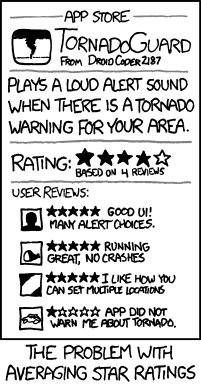
\includegraphics[width=\textwidth]{images/xkcd/tornadoguard.png}
  \captionof*{figure}{TornadoGuard \url{https://xkcd.com/937}}
  \label{fig:xkcd-tornadoguard}
\end{minipage}\hfill%
\begin{minipage}{.5\textwidth}
  \centering
  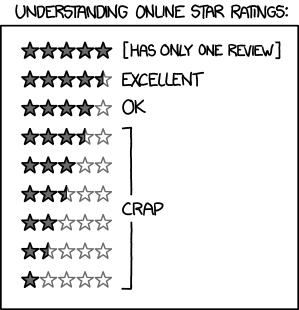
\includegraphics[width=\textwidth]{images/xkcd/star_ratings.png}
  \captionof*{figure}{Understanding online star ratings \url{https://xkcd.com/1098}}
  \label{fig:xkcd-star-ratings}
\end{minipage}
    \caption{XKCD's views on App Store Ratings and Reviews}
    \label{fig:xkcd-app-store-ratings}
\end{figure}
% https://www.explainxkcd.com/wiki/index.php/937:_TornadoGuard
% https://www.explainxkcd.com/wiki/index.php/1098:_Star_Ratings


Apps with poor ratings are less likely to be downloaded by new users~\sidecite{dimensionalresearch2015_mobile_app_use_and_abandonment}. Ratings also affect where an app appears in search results and whether an app store will choose to promote that app, or another. In the author's experience when one team's Android app's overall rating dropped from 4.4 to 4.3 stars the business noticed an almost immediate reduction in revenues from the app in addition to discovering that app was ranked lower in the search results. Therefore ratings are an important measure for app developers, and one they may choose to influence positively. 

Gaming ratings includes activities such as an app first asking if a user is happy with the app, and if they say yes then providing a link to encourage the user to rate the app positively in the app store. \textcite{novoda_akan2016_asking_for_app_feedback_the_effective_way} provides an illustrative industry case study of how Novoda improved the rating of a major newspaper's app. And in terms of the SDKs developers can use for in-app feedback, Apptentive is one of several companies that provides SDKs to help developers optimise their ratings and reviews and guides on how to do so within a mobile app~\sidecite{walz2015_apptentive_the_mobile_marketers_guide_to_app_store_ratings_and_reviews}. Unsurprisingly, ratings are also a subject of research interest.

Here are several representative papers that focus on engineering aspects of ratings and reviews.  \textcite{alsubaihin2019app_store_effects_on_software_engineering} discusses the symbiotic relationship between releases and the ratings and reviews that app received [p. 14]. Some developers time their releases based on the feedback they've received and monitor ratings and reviews for their latest release to influence the rollout of the new release. There have been innovative ideas on using ratings to prioritise software engineering activities including software testing of Android games apps~\sidecite{khalid2014_prioritizing_the_devices_to_test_your_app_on_casestudy_android_games}. And in \textcite{greenheld2018_automating_developers_responses_to_app_reviews} the value of developers responding to reviews was highlighted. 
In a population of 10,000 Android apps extracted from Google Play, correlations was identified between the density of warnings reported by FindBugs, a static analysis tool, and app store reviews and ratings for these apps~\sidecite{khalid2016_examining_the_relationship_between_findbugs_warnings_and_app_ratings}. They considered three warning categories: bad practices (which include reports of crashes in the reviews), internationalisation, and performance (which might relate to ANRs, however they didn't investigate this aspect). They did not investigate whether addressing warnings from FindBugs improved the ratings or reviews for those apps, and mobile analytics was not mentioned in their work - unsurprising as they took a black box approach using decompiled Android app binaries.

Via Figure \ref{fig:xkcd-app-store-ratings} XKCD aptly sums up two facets of flaws in app store ratings and reviews, averaging reviews may not be a good measure~\sidecite{explainxkcd_937_tornadoguard}, and the star ratings are not treated as a linear scale in practice~\sidecite{explainxkcd_1098_star_ratings}. In summary, app Store ratings therefore may not be an ideal measure of the quality of an app from a software engineering perspective! 
% See also stanik2020_requirements_intelligence_on_the_analysis_of_user_feedback
% shen2017_towards_release_strategy_optimization_for_apps_in_google_play 

\subsection{Reviews in app stores}
Similarly reviews in app stores have been analysed for various purposes including for complaints and bug reports. Of the many and various research on reviews of mobile apps in app stores. 
Two early papers, the first focusing on Android apps in Google Play~\textcite{fu2013_why_people_hate_your_app_making_sense_of_user_feedback_in_a_mobile_app_store} and the second for iOS apps in Apple's App Store~\textcite{khalid2015_what_do_mobile_app_users_complain_about}.

In \textcite[p. 5][]{fu2013_why_people_hate_your_app_making_sense_of_user_feedback_in_a_mobile_app_store} the top three most common indicators of problems in the apps were: slow 9,939, crashes 9,081, and freezes 3,960. Stability was a common theme of complaints about both free and paid apps [pp. 7-9]. 

In \textcite{khalid2015_what_do_mobile_app_users_complain_about} clearly establishes connections between what users of iOS apps complain about and the effects of these complaints on ratings of those apps; and \textcite{panichella2015_how_can_i_improve_my_app_classifying_user_reviews_for_sw_maintenance_and_evolution} extends that work to consider the relevance of various review-topics to developers. Panichella \emph{et al} also extend the work to include Android apps in the Google Play Store. \textcite{mcilroy2016_analyzing_and_automatically_labelling_the_types_of_user_issues_raised_in_mobile_app_reviews} - labels the content of reviews extracted from Google Play and found crashes and crashing were one of the topics that was a) relatively easy to categorise, and b) occurred frequently. This paper seemed to conflate in-app analytics tools (Flurry) with analytics of reviews (e.g. AppAnnie). As an observation, since this paper was published Google Play now provides automated labeling and analysis of reviews.

Feedback comes in various forms, ratings and reviews are only two of them.  One that's seldom used in industry and seldom researched is implicit feedback recorded through user-interactions with the GUI of the mobile app. Common terms for this mechanism include `heatmaps' and `heatmapping' and there are commercial SDKs and opensource projects available that perform the recording within an app at runtime. The elixir of automating `record and playback' test automation sometimes uses similar methods to record the interactions with a mobile app. 

\subsection{Testing}
\emph{``How do Developers Test Android Applications?"}~\sidecite{linares2017_how_do_developers_test_android_apps}. Quote:~\emph{``“I mostly do manual testing due to the limited size of my apps. I sometimes use a custom replay system (built into the app) to duplicate bugs after I come across them. This method is usually combined with manual testing (printing debug information to the log) to pinpoint the cause”."}

The absence of automated tests does not prove developers do not test their Android apps, rather it indicates their projects are unlikely to have any automated tests and similarly that the project is unlikely to run any automated scripted tests as part of a continuous build. (In honour of Dijkstra's observation that ``Testing shows the presence, not the absence of bugs'', Edsger W. Dijkstra in ~\textcite[p. 16][]{randell1970_software_engineering_techniques_nato_dijkstra}.) % Found via https://en.wikiquote.org/wiki/Edsger_W._Dijkstra
% See also: https://www.techwell.com/techwell-insights/2018/12/can-we-ever-find-all-bugs 
% https://wiki.c2.com/?TestsCantProveTheAbsenceOfBugs

An incredible amount of research energy has gone into trying to find better ways to test mobile apps, ranging from autonomous tools that where the researchers endeavour to deliver better coverage than a small free utility called \texttt{monkey} (and sometimes manage to do so), through to ways to generate automated tests from the text of reviews. Virtually none of these endeavours seem to make any difference to the testing developers do, they don't use the tools developed from these research efforts. 

\emph{``Thus even if the app is tested on one device, there is no guarantee that it may work on another device."}~\cite[p. 27]{nagappan2016_future_trends_in_sw_eng_for_mobile_apps} - I agree. They don't provide any substance for this statement.

research gaps...

And yet, researchers also continue to complain app developers don't test their apps sufficiently. They sometimes berate the app developers to `test their apps' ,\emph{e.g.}~\textcite{cruz2019_guess_what_test_your_app}.
Similarly the voices of the researchers seem to go unacknowledged and unapplied.

Another strand is where researchers collate examples of apps together with faults they have identified and analysed in order to help, primarily, other researchers. 

Why are all these efforts to improve software testing for mobile apps generating seemingly minimal effects in practice? Perhaps researchers into improving mobile apps would find an approach similar to the research of~\textcite{winter2022_lets_talk_with_developers_etc_automatic_program_repair} more productive - by actually talking \emph{with} the app developers and then offering to research pain points identified by those app developers. Doing so might increase the external and ecological validity of the research and potentially also increase the adoption of the research. The adoption might be at an individual developer, team, or organisation level. In some instances the effects of the research may gain wider adoption and become a tool, technique, approach that many app developers adopt. In some cases the app store and/or platform provider might also adopt the work, for instance to replace their current `monkey' test tool. As an aside Google already has replaced their `monkey' utility with `robo'.

Developers do want automated tests and tools to provide them with feedback~\cite[p. 5]{greiler2022_an_actionable_framework_for_understanding_and_improving_developer_experience} even if relatively few projects have sufficient tests to provide the developers with a level of comfort and confidence. Again, much of the research has focused on where researchers can find tests rather than working with development teams to understand their desires and the barriers that mean the developers don't have (m)any tests. 

For project teams with large volumes of automated tests, what value do those tests provide? Fortuitously one of the app-centric case studies, Catrobat, has an opensource codebase and their uses of automated tests are well researched. The Catrobat project makes extensive use of various forms of automated tests including using Behaviour-Driven-Development (BDD) practices~\textcite{ali2019using_catrobat}, testing under adverse conditions~\textcite{adamsen2015systematic_catrobat}, the use of sizing for automated tests~\textcite{hirsch2019approach_catrobat}, \emph{etc}. % TODO add additional references for Catrobat. See the findings-results chapter.

\subsection{Mobile Analytics}
In-app analytics have been used to help developers understand ways their mobile app is used by large populations of end-users and the effects of various conditions on the behaviours of the end users. There has been some research into using mobile analytics to understand usage patterns of specific apps, for example:

\begin{itemize}
    \item \textcite{parate2016_RECKON_an_analytics_framework_for_app_developers_HP_AppPulseMobile} describes how automatic instrumentation of mobile apps using mobile analytics tools including HP's App Pulse Mobile is able to help developers better understand their users.
    \item \textcite{ferre2017_extending_mobile_app_analytics_for_usability_test_logging} identified the importance of usability testing in terms of success of mobile apps, while there are challenges and severe limitations with usability testing in the lab. This research evaluated the use of Google Analytics for Mobile Applications to provide continuous usability logging. They describe a three-stage proposed approach to logging. In the third stage they have two alternatives, one for lab usability testing, the other for continuous usability logging.
    \item and the Insight toolkit~\textcite{patro2013_capturing_mobile_experience_in_the_wild} which is covered in more detail next.
\end{itemize}   

Two mobile apps incorporated a toolkit library called Insight~\cite[p. 82]{patro2015_building_blocks_to_understand_wireless_experience}~\footnote{Interim aspects of this research was also published~\textcite{patro2013_capturing_mobile_experience_in_the_wild}.} that combined passive analytics, such as session length, with factors, such as network condition and client device, with the aim of helping the developers recognise correlations between these factors and application use and revenues[p. 82](\textit{ibid}).

The research describes generic data, collected by Insight for any app, and app-specific data, which is defined and implemented by the developers of that app~\cite[pp. 87-88]{patro2015_building_blocks_to_understand_wireless_experience}. They identified a correlation between battery drain and session lengths, as battery drain increased the session lengths decreased, and also the correlation between screen brightness and battery drain. The device model was a material factor in the rate the battery drained, and in particular on Kindle Fire devices the drain was far higher when the screen was bright. ``\emph{controlling the screen brightness on a Kindle Fire device reduced the average battery drain by 40\% while using SB}''~\cite[p. 13]{patro2015_building_blocks_to_understand_wireless_experience} Note: SB is short for StudyBlue, one of the two apps in this study.

The research using Insight was one of the catalytic agents for this research as it was able to publish data obtained using mobile analytics for two popular real-world apps. They also made both their client and server code freely available online as opensource projects: \url{https://github.com/patroashish/InsightClient} and \url{https://github.com/patroashish/InsightServers}. Although they mention they developed an iOS SDK it does not appear to have been made available online~\cite[p. 85]{patro2015_building_blocks_to_understand_wireless_experience}.

Perhaps paradoxically the Insight client SDK, freely available at \url{https://github.com/patroashish/InsightClient}, does not record or report any failures of the SDK or of the associated app it has been integrated with. Assuming crashes, freezes, and other similar issues might affect the end-user experience it seems odd the SDK doesn't track these aspects. Furthermore the SDK only sends the analytics data when there is a working mobile network immediately available, it does not appear to queue events, incorporate any robustness mechanisms, or include any re-transmission capabilities.

With the exception of a brief comparison between Insight and three then popular mobile analytics services their research does not investigate any other mobile analytics offering.

Note: there has also been research into similar sounding work on software analytics for mobile apps~\textcite{minelli2013_software_analytics_samoa}, however that research is into characteristics of the source code rather than in the use of mobile analytics by app developers.

Research into mobile analytics is surprisingly rare, especially given the prevalence of apps that include mobile analytics SDKs and their use by mobile app developers. A possible reason for the rarity is the challenges in researchers obtaining access to the outputs of the mobile analytics. For the research using Insight they negotiated special non-disclosure agreements (NDAs) and the data was pre-filtered to increase the privacy of the end users~\cite[p. 91]{patro2015_building_blocks_to_understand_wireless_experience}. 

Before we leave the topic of mobile analytics research into the privacy aspects of the mobile analytics SDKs is pertinent as the choices developers make in terms of selecting in-app mobile analytics has various consequences including the privacy for the end users who indirectly provide the underlying data. Two illustrative areas of research into the privacy and data leakage aspects are:

\begin{itemize}
        \item \textcite{razaghpanah2018_apps_trackers_privacy_and_regulators_a_global_study_of_the_mobile_tracking_ecosystem} where a privacy-focused app is used to obtain the network traffic sent to ad and analytics end points from end-user devices. That traffic is analysed to understand where it goes, who has access to the underlying data, and what of the content is most likely to contravene ePrivacy and GDPR directives.
        \item \textcite{liu2020_privacy_risk_analysis_and_mitigation_of_analytics_libraries_in_the_android_ecosystem}, in contrast, modifies the binary files of various apps in order to intercept the calls to the respective in-app SDKs of various mobile analytics libraries. They developed a proof-of-concept Android app AlManager that a) allows the user to see the contents of the calls made to the in-app SDKs, and b) to block or replace the contents with blank data. They also studied characteristics of the calls the apps made in terms of the App, Activity, and User level in terms of the data being sent to the mobile analytics SDK(s).
\end{itemize}

The first of these papers focuses on the data that is sent, the contents, and where that data goes. The second concentrates on analysing app binaries, finding all the calls to the mobile analytics SDKs, intercepting these and enabling users to see, block or blank out data that would then be sent by the respective mobile analytics SDK.


\section{Mobile App Crashes}~\label{rw-mobile-app-crashes-topic}
Crashes in mobile apps have garnered a great deal of research, perhaps as crashes are definitive and relatively easy to detect.

There is some interesting large-scale research into analysis of various releases of production Android application binaries~\sidecite{kong2019_mining_android_crash_fixes}. The researchers exercised (tested) a large range of apps seeking crashes of the app using an oracle of a local log file which they queried using the standard Android \texttt{logcat} utility. They also combined their dynamic approach with using static analysis tools to identify potential flaws that would lead to crashes of an app. They then tested newer releases of the same app. If the newer version did not crash they analysed the binary files (the APK files) for both releases to differences to the compiled code that may have been responsible for 'fixing' the crash. They limited their work to Android \emph{framework specific} crashes, and excluded \emph{app-specific} crashes. They devised ways to identify changes that appeared to fix the particular crash(es) they triggered in the earlier releases and generated patch files based on these changes. These patches were then applied to the older release of the app and the app then tested with the same test inputs and runtime environment (at least in terms of using a consistent Android Emulator (also known as a virtual device)). They provide a relatively detailed replication package online at~\url{https://craftdroid.github.io/}.

\begin{itemize}
    \item Their approach is innovative and could help real-world developers of Android apps to identify and apply snippets of code to reduce the likelihood of their app suffering the same crash. Their 17~\href{https://github.com/CraftDroid/ExpData/tree/master/Fix_Templates}{fix templates} act as guides for Android developers and could potentially be implemented into code-quality tools.
    \item However it only applied for framework specific crashes, and their choice of runtime environment meant they could only install 56\% of the APKs. There are many other sources of crashes, and also apps that include native code (several of my case study apps do). Also their testing is limited to automated `monkey' testing which may further limit the crashes their approach can find in production apps, particularly those that incorporate user accounts, user-specific content, behaviour, online purchases and many other forms of activities.
    \item The supporting website \url{https://github.com/CraftDroid} includes scripts and log extracts for the crash reproductions, it lacks the mechanisms for generating diffs, applying them, or building the patched APK. The lack of these mechanisms makes the efficacy of their approach hard to reproduce.
    \item It also does not appear to test for crashes related to third-party libraries e.g. OkHttp which is extremely popular in Android apps; however potentially this approach could be extended to do so?
\end{itemize}

In summary, the approach proposed in~\sidecite{kong2019_mining_android_crash_fixes} has the potential to mine crash stack traces (which are available to the developers of the particular apps) to help with aspects of reproducing a subset of those crashes which pertain to Android framework-related crashes. Similarly it appears it could complement the automated testing provided by Google as part of the pre-launch reports available in Google Play Console and other services. 

In contrast, ~\sidecite{wang2018_an_empirical_study_of_android_test_generation_tools_in_industrial_cases} evaluated a mixed set of industrial and opensource test automation tools against popular Android apps available in Google Play. They measured code coverage and the count of unique crashes each tool could find in these apps. They also considered more practical aspects such as finding ways to combine tools to increase the code coverage and fault detection, they also measured the effort required to setup each of the tools to test the industrial apps. Their reference tool was Android `Monkey' the ubiquitous tool shipped with the Android SDK and one of the most widely used of these tools. This research appears practical and well grounded. It does not compare any aspect of crashes in the wild \emph{i.e.} those that affect end users and some of the crashes that were detected, such as those reported when Sapienz was used to test the Wattpad app might have established sufficiently unusual conditions for those crashes to be unlikely for most end users. (Nonetheless these crashes might still be of interest to the app's developers). 

The authors did not mention whether they reported the crashes to the app developers, which is a pity as it would have been interesting to learn whether the app developers were willing and able to fix the crashes. If the researchers had reported the crashes to the app developers then this research - if combined with the research in the previous paper~\sidecite{kong2019_mining_android_crash_fixes} - could have been enlightening to measure at a black box level whether the crashes had been successfully fixed post reporting them.


\section{Summary so far} % Or curiosities, or gaps in the research at this stage...?
App stores, their ecosystems, and their effects on developers have been covered from various angles. Some of the research describes snapshots of one or more app stores. And some of the research involves developers of live apps in a mainstream app store. Ratings and reviews are covered from many angles including fraud~\sidecite{xie2015_appwatcher_unveiling_the_underground_market_of_trading_mobile_app_reviews}. 

One of the curiosities reported in~\textcite{alsubaihin2019app_store_effects_on_software_engineering} is: \emph{``while automatic in-app crash reporting is the most prolific channel of reporting bugs, the one mostly prioritised by our respondents is user reviews in app stores."}[p. 13] - what are the effects of the crashes being a lower priority than user reviews? Also, they don't discuss other sources of crash reports (e.g. platform crash reporting) even though these existed at the time of their research.

Similarly, in terms of managing releases in app stores, the platform provided release management tools and reports were not mentioned. 

Several points made in \sidecite{frankl1997choosing_testing_for_reliability} discuss the potential perils of relying on the judgement of people involved in debug testing (testing to maximise the faults found in a given period), the first point is based on work by \sidecite{basili1994_software_process_evolution_at_the_sei} where testers who focused on `testing' over estimated their abilities to find all the faults in a program, by proposing it is possible to compare the effectiveness of testing by using operational profiles~\sidecite[][p. 77]{frankl1997choosing_testing_for_reliability}.

The second point is there is the potential for debug testers to confuse \emph{``between detecting failures and achieving reliability.''}~\sidecite[][p. 77]{frankl1997choosing_testing_for_reliability}. Mobile Analytics might be able to provide a real-world measure in terms of achieving reliability. Furthermore, much of the research into mobile app crashes seems to end prematurely - before considering whether reliability of the app has been improved by whatever method and approach they have researched.

\begin{quote}
    \emph{``...with explicit and implicit feedback now available (almost) continuously, questions arise. How can practitioners use this information and integrate it into their development processes to decide when to release updates?''}\cite[pp. 48-49]{maalej2016_towards_data_driven_requirements_engineering}    
\end{quote}

Building on a point made in this paper: \emph{``the future of app quality engineering is data driven."}~\cite[p. 24]{nagappan2016_future_trends_in_sw_eng_for_mobile_apps} % cite 97.


\julian{TODO complete this thought: However none of these (these researches) provide X which is my need...}
\setchapterpreamble[u]{\margintoc}
\chapter{Overview of the case studies}~\label{chapter-case-studies-overview}

This chapter introduces each of the app-centric and tool-centric case studies using a consistent structure to make them easy to comprehend and to facilitate comparison. The depth of each section varies to focus on material that's of consequence to the thesis. 

The case studies are in three groups, with a couple of interim sections that present complementary research that helps to fill various gaps. These three groups are: 
\begin{enumerate}
    \itemsep0em
    \item[1] App-centric case studies that \textbf{do not} have interventions (Sections \ref{case-study-overview-gtaf}, to \ref{case-study-overview-smartnavi}).
    \item[2] App-centric case studies that \textbf{do} have interventions (Sections \ref{case-study-overview-kiwix} to \ref{case-study-overview-C1}).
    \item[ ] Interim work on various field experiments (Section \ref{section-field-experiments-to-augment-app-centric-case-studies}) and source code analysis (Section \ref{section-sourcecode-analysis-to-augment-app-centric-case-studies}).
    \item[3] Tool-centric case studies (Sections \ref{case-study-overview-crashlytics} to \ref{case-study-overview-sentry}).
    \item[ ] Section \ref{section-case-study-misc-contributions} briefly introduces six more mobile analytics tools and another Android app as these provide miscellaneous minor contributions in the subsequent three chapters.
\end{enumerate}

The app-centric case studies are presented in the same order as Table~\ref{tab:app-centric-studies-research-perspective} for the app-centric cases and then Table~\ref{tab:tool-centric-studies-research-perspective} for the tool-centric cases. 

The structure used to present each app-centric case study includes two summary tables. The first presents the key-facts pertaining to that case study, the second table presents the data sources. These are augmented with brief descriptions. 

\begin{comment}

covers the following topics:
\begin{itemize}
    \itemsep0em
    \item \textbf{Organisation overview:} including an overview of the development team and practices.
    \item \textbf{Engagement:} my involvement and the timescales.
    \item \textbf{Data/methods:} a summary of the data collected and methods used for the data collection based on Table~\ref{tab:mapping-datasources-to-six-perspectives}, including any intervention.
    \item \textbf{Contributions to the research} and where they are located in the rest of this dissertation.
\end{itemize}
\end{comment}

Each of the overviews for the tool-centric case studies includes a table with the key-facts augmented with a contextual summary together with the data collected and methods used for collecting material for this mobile analytics tool.

The nature of the case studies means they include observations and findings that occurred at the time. There may be situations where there are differences between these observations and findings and those of other users of these tools. 
\clearpage



%===================================================================

\section{App-centric: GTAF}~\label{case-study-overview-gtaf}
% A couple of sentences to introduce them
\Acrfull{gtaf}\index{GTAF} is a UK-based charity that provides Islamic apps free of charge and without in-app advertising. The project started in 2016 with the aim of enabling people to learn the Quran in the local language -- Bangla -- in Bangladesh. The project was started by a self-taught Android developer and his cousin Yemin, at the time an undergraduate student in computer science, who is now employed by the project in a hybrid role of software developer and project manager. Table \ref{tab:gtaf_anaytics_overview} summarises the key facts for this case study.

{\renewcommand{\arraystretch}{0.8}% Tighter
\begin{table*}
    \centering
    \small
    \setlength{\tabcolsep}{6pt}
    \begin{tabular}{lp{11cm}}
       % Question &Answer  \\
       \toprule
       Website &\url{https://gtaf.org/} \\
       Google Play Home & \url{https://play.google.com/store/apps/dev?id=7665838187257770408} \\
       Founded & 2016 \\
       Business Domain & Not-for-profit.  \\
       Business type & Educational foundation. \\
       Technologies  & Android apps\footnotemark \\
       & React Native \\
       Source code  & Closed and not available for research \\
       Analytics used by team & Firebase, OneSignal, Google Crashlytics, Google Play Console \\
       Development Practices & Small hybrid development team \\
       \midrule
       User base & 1,000,000'+ for their 10 Android apps \\
       Installations & 1,000,000's for their 10 Android apps \\
       \midrule
       Source of case study &Via a fellow PhD researcher who was a software developer on the project. \\
       Catalyst for the case study &Excessively high crash rates for several of their apps piqued their interest in the research. \\
       \midrule
       Research methods &Online interview and email discussions, etc. \\
       Analytics collected &Google Play Console with Android Vitals \\
       Research software & None applicable? \\
       Additional data collected &Direct access to Google Play Console with Android Vitals, and to the public, issue database. Interview notes and emails. \\
       Active period & June 2020 to September 2020 \\
       \midrule
       \emph{Post-hoc} analysis &Included ongoing access to their Google Play Console for 18 months. \\
       \bottomrule
    \end{tabular}
    \caption{Case Study key facts: \acrshort{gtaf}}
    \label{tab:gtaf_anaytics_overview}
\end{table*}
}

\footnotetext{The project have subsequently released several of their apps on other platforms, see \url{https://gtaf.org/apps}.}

% \subsection{GTAF: development microcosm} 
The project team hosts their development artefacts on gitlab.com, and they maintain their issues in a publicly-available online database at \url{https://gitlab.com/greentech/}; the source code is private. There is a mix of paid developers (through donations to the charity) and volunteers (often part-time). The developers of some of the less-active apps appear relatively autonomous, which includes their choice and any use of mobile analytics. 

Three of the apps (effectively four, because one app is released as two distinct binaries) were in ongoing active development (\href{https://play.google.com/store/apps/details?id=com.greentech.quran}{Al Quran},~\href{https://play.google.com/store/apps/details?id=com.greentech.hadith}{Hadith Collection}, and~\href{https://play.google.com/store/apps/details?id=com.greentech.hisnulmuslim}{Dua \& Zikr}, which is also released separately in Bangla~\href{https://play.google.com/store/apps/details?id=com.greentech.hisnulmuslimbn}{{Dua and Zikr (Hisnul Muslim)}}~\emph{in Bengali}); and they planned to revamp two more of the apps (\href{https://play.google.com/store/apps/details?id=com.greentech.islamicquiz}{(Islamic Quiz)} and~\href{https://play.google.com/store/apps/details?id=com.greentech.salatbn}{Meaningful prayers (salat)}~\textit{in Bengali}. %, which was called salat in our interview).

The team occasionally used Firebase TestLab~\footnote{\url{https://firebase.google.com/docs/test-lab}} to test some of the apps, and autonomous `Robo testing'~\footnote{\url{https://firebase.google.com/docs/test-lab/android/robo-ux-test}}, performed automatically by the test lab, triggered various crashes in the apps being tested. One such example was where an app was missing a `resource'. The team fixed the build by adding the missing resource but did not explicitly retest the app afterward in Firebase.  

\textbf{Data sources:} the data sources obtained in this case study are illustrated in Table~\ref{tab:gtaf-data-sources}.

\begin{table*}
    \centering
    \footnotesize
    \tabcolsep=0.12cm
    \begin{tabular}{p{2.4cm}p{2.4cm}r>{\raggedright}p{2.4cm}>{\raggedright}p{3cm}>{\raggedright\arraybackslash}p{2.5cm}}
        Data Source & Records & Volumes & Analysis method &Contribution & Remarks \\
        \toprule
         Pre-study interview, with core developer & contemporaneous notes\footnotemark & 1 & Ask the app devs & Set scope \& direction & Online call \\
         Analytics tools \& artefacts &Interactive screenshots \& Vitals-scraper outputs &10\textsuperscript{1} & Beacon finding, drill down, across case comparisons, observation \& analysis. & Indications of the development team's attention to the crash rate, insights into the performance of their apps, corroboration of findings across various case studies. & Google Play Console with Android Vitals. \\         
         Mid-study communications with developers & GMail & 10\textsuperscript{1} & Ask the app devs & Feedback, and sense-making.  & Email conversations. \\
         Development artefacts  & Issues database & 10\textsuperscript{2} & Observation and Analysis, analysis of development artefacts. & Corroboration of what the development team say they do in terms of using mobile analytics. & Public GitLab repo. \\
         \bottomrule
    \end{tabular}
    \caption{GTAF: data sources}
    \label{tab:gtaf-data-sources}
\end{table*}


\textbf{GTAF: Contributions to the research}
TBC\todo{Add forward links when the relevant material has been included.}.


%\clearpage

%===================================================================

\section{App-centric: Local Halo}~\label{case-study-overview-localhalo}
LocalHalo\index{LocalHalo} was a startup based in London who made a social network for neighbours~\footnote{\url{https://ain.ua/en/2019/10/18/localhalo-raises-500k/}} with developers in Ukraine, London, and Kazakhstan.~\sideparencite{karpenko2019_localhalo_a_social_network_for_neighbors}. 
Table~\ref{tab:local_halo_anaytics_overview} provides an overview of this case study.

The development team used the Expo development platform \url{https://expo.dev/} to create native apps that ran on Android and iOS apps. The mobile app was written in React Native~\footnote{\url{https://reactnative.dev/}} (the associated website is likely to have been written using React js~\footnote{\url{https://reactjs.org/}} and also instrumented using Sentry Analytics which were also available for research purposes). These apps were released on Google Play and Apple's App Store respectively. The \acrshort{cto} was actively involved in writing and maintaining the source code and was supported by developers in three locations, in the Ukraine, London, and Kazakhstan.~\sideparencite{karpenko2019_localhalo_a_social_network_for_neighbors}.  Data in the Sentry mobile analytics reports indicate there was at least one distinct developer in addition to the CTO.

Little additional information was available during conversations in terms of their development or release practices for their mobile apps. One observation is Expo claims to automate the release process to the app stores so the LocalHalo development team may have relied and used the Expo service. And Sentry provided reports on the release numbers and their rollout.

{\renewcommand{\arraystretch}{0.8}% Tighter
\begin{table*}
    \centering
    \small
    \setlength{\tabcolsep}{6pt}
    \begin{tabular}{lp{11cm}}
       % Question &Answer  \\
       \toprule
       Website &\url{https://www.localhalo.com/} \\
       Google Play Home & \url{https://play.google.com/store/apps/developer?id=NAY+PROTECT+LTD} \\
       Founded &2018 \\
       Business Domain &Digital neighbourhood groups in UK.\\
       Business type &Startup, two co-founders: CEO and \acrshort{cto} \\
       Technologies  &React Native for cross-platform Android and iOS development \\
       &Expo development framework \\
       Source code  &Closed and not available for research \\
       Analytics used by team &Sentry, Mixpanel, Google Play Console \\
       Development Practices &Not explicit, a small distributed team \\
       \midrule
       User base &7,000 registered users and between 1k to 2k monthly active users in Jan 2020. \\
       Installations &1,000's for the Android app \\
       \midrule
       Source of case study &One of their team knew of my professional work and introduced me to the CEO. \\
       Catalyst for the case study &The CEO was keen to support the research. \\
       Approvals &Internally approved within the core development team. \\
       \midrule
       Research methods &Interview, email discussions, bug analysis, use of mobile analytics \\
       Analytics collected &Live access to: Sentry, Google Play Console with Android Vitals \\
       Research software &Vitals-Scraper used to preserve results \\
       Additional data collected &Interview notes, emails with the \acrshort{cto}, and automated emails from their mobile analytics services \\
       Active period &Jan 2020 to June 2020 \\
       \midrule
       \emph{Post-hoc} analysis &Included ongoing access to Sentry until late 2021. \\
       \bottomrule
    \end{tabular}
    \caption{Case Study key facts: Local Halo}
    \label{tab:local_halo_anaytics_overview}
\end{table*}
}

\textbf{Data sources:} Table~\ref{tab:localhalo-data-sources} provides details of the data sources obtained during this case study.

\begin{table*}
    \centering
    \footnotesize
    \tabcolsep=0.12cm
    \begin{tabular}{p{2.4cm}p{2.4cm}r>{\raggedright}p{2.4cm}>{\raggedright}p{3cm}>{\raggedright\arraybackslash}p{2.5cm}} % Fixed thx to https://tex.stackexchange.com/a/467120/88466
        Data Source & Records & Volumes & Analysis method & Contribution & Remarks \\
        \toprule
         Pre-study interviews & contemporaneous notes\footnotemark & 3 & Ask the app devs. & Set scope and direction & 1-to-1 meetings with founders: 1 was in-person, 2 were online. \\
         Mid-study communications with developers & GMail & 10\textsuperscript{1} & Ask the app devs. & Insight into the Expo bug & Initiated by the researcher. \\
         Analytics tools \& artefacts &Interactive screenshots \& Vitals-scraper outputs &10\textsuperscript{1} & Beacon finding, drill down, across case comparisons, observation \& analysis. & Insight into the reporting effects of the Expo bug and the reporting provided for React-Native apps & Google Play Console with Android Vitals. \\
         Analytics tools \& artefacts & Interactive screenshots of the Sentry \acrshort{gui} & 10\textsuperscript{1} & Beacon finding, drill down, across \textit{tool} comparisons\footnotemark, observation \& analysis. & Insights into Sentry's reporting & Access continued until Sentry removed multi-account access from their free tier. \\
         Analytics tools \& artefacts & Sentry automated emails in GMail & 10\textsuperscript{2} & Beacon finding, drill down, observation and analysis. & Insights into Sentry's reporting, dev practices, \& cross-platform reporting & \textit{ditto.} NB: they continue to send weekly reports by email. \\
         \bottomrule
    \end{tabular}
    \caption{LocalHalo: data sources}
    \label{tab:localhalo-data-sources}
\end{table*}

\footnotetext{Pertinent details validated by email.}
\footnotetext{A specialisation of across case comparisons where the outputs of two mobile analytics tools were compared.}


\textbf{Local Halo: Contributions to the research}
TBC\todo{Add forward links when the relevant material has been included.}.

%\clearpage

%===================================================================

\section{App-centric: Moodspace}~\label{case-study-overview-moodspace} % The title is used throughout this file, do a search and replace.
Moodspace\index{Moodspace} is an Android app aimed at improving mental health through various exercises incorporated into the app. %The app was listed as one of the 25 best mental health apps~\footnote{\url{https://www.psycom.net/25-best-mental-health-apps}}. 
% The app features in various peer-reviewed papers, however they lack critical depth of the app e.g. in https://doi.org/10.1145/3411764.3445500 
%  -- ``A systematic review of cognitive behavioral therapy and behavioral activation apps for depression" (PLoS 2016)
% -- https://www.ncbi.nlm.nih.gov/pmc/articles/PMC8529472/ (and the DOI https://mhealth.jmir.org/2021/10/e26712 )
% -- The following paper explains the needle-in-a-haystack challenge of establishing the evidence for this and similar apps https://www.ncbi.nlm.nih.gov/pmc/articles/PMC7588098/
% It also features online e.g. in https://www.healthfoundry.org/covid-19-response 
It was released in 2019, with over 150K downloads by early 2020~\sideparencite{objectbox2020_moodspace_interview}. Ian Alexander, the interviewee, was `the software developer, co-founder, and runner of the company'~\sideparencite{objectbox2020_moodspace_interview} so he combined technical and operational responsibilities in his \Gls{cto} role. He is an experienced app developer and also trained as a chemical engineer. The \Gls{cto} was the sole developer. 

{\renewcommand{\arraystretch}{0.8}% Tighter
\begin{table*}
    \centering
    \small
    \setlength{\tabcolsep}{6pt}
    \begin{tabular}{lp{9cm}}
       % Question &Answer  \\
       \toprule
       Website &\url{https://moodspace.org/} \\
       Google Play Home & \url{https://play.google.com/store/apps/details?id=boundless.moodgym} \\
       Founded & 2019 \\
       Business Domain & Health \\
       Business type & Online, in-app purchases. \\
       Technologies  & Android \\
       & ObjectBox ORM database \\
       Source code  &Closed and not available for research \\
       Analytics used by team & Firebase Analytics, Firebase Crashlytics, Google Play Console \\
       Development Practices & Sole software developer \\
       \midrule
       User base & 10,000's for the Android app \\
       Installations & 100,000's for the Android app \\
       \midrule
       Source of case study &One of their team knew of my professional work and introduced me to the CTO. \\
       Catalyst for the case study &The CTO was happy to support the research. \\
       Approvals &Directly from the interviewee, the \Gls{cto}. \\
       \midrule
       Research methods &Email interview \& follow-up discussions. \\
       Analytics collected &Google Play Console with Android Vitals \\
       Research software & None applicable. \\
       Additional data collected &Exodus Privacy project reports. \\
       Active period & June 2019. \\
       \midrule
       \emph{Post-hoc} analysis &Material provided during the active period was combined with additional Grey Material, particularly for objectbox, an in-memory ORM database used in the app. \\
       \bottomrule
    \end{tabular}
    \caption{Case Study key facts: Moodspace}
    \label{tab:moodspace_case_study_anaytics_overview}
\end{table*}
}

The source code, issues database, and mobile analytics were all private.

At the time of the interview the team had developed a complete replacement for the Android app which was due to be launched in a couple of months (around August 2019). The startup was subsequently able to raise a round of funding and grow to six people. The project later returned to be a side-project which is maintained and updated~\sideparencite{alexander2021_linkedin_profile}.

The app had a strong positive User Experience rating of 4.18/5.00~\footnote{\url{https://onemindpsyberguide.org/apps/moodspace/}} which corroborates their objective to provide a beautiful and peaceful mobile app.

\textbf{Data sources:} Table~\ref{tab:moodspace-data-sources} provides details of the data sources collected in this case study.

\begin{table*}
    \centering
    \footnotesize
    \tabcolsep=0.12cm
    \begin{tabular}{p{2.3cm}>{\raggedright}p{2.1cm}r>{\raggedright}p{2.4cm}>{\raggedright}p{2.8cm}>{\raggedright\arraybackslash}p{3.2cm}}
        Data Source & Records & Volumes & Analysis method & Contribution & Remarks \\
        \toprule
         Pre-study interview \&Mid-study communications with developers & GMail & 10\textsuperscript{1} & Ask the app devs. & Effectively the interview, albeit using emails.  & We ended up simply using emails rather than arranging a synchronous call and then continued the discussion using email.  \\
         Analytics tools \& artefacts &Interactive screenshots & 6 & Ask the app devs. & Evidence, and allows for comparisons. & Google Play Console with Android Vitals \\
         Grey Data &Tweets & 3 & Grey Data & Triangulation & The app was made fully free in response to the Covid-19 pandemic. \\
         \textit{Academic} Literature  &Peer reviewed publications & 3 & Secondary research. & Additional context & The app has been studied in various peer-reviewed papers.\footnotemark \\
         Grey Literature &Online articles & 10\textsuperscript{1} & Secondary research & Additional context & There are various discussions about the efficacy and suitability of this and similar apps. \\
         Development artefacts\footnotemark & Exodus Privacy project online reports & 4 & Grey Data & Details of mobile analytics integrated into the app & Their 4 snapshots indicate a variety of mobile analytics have been incorporated~\footnotemark. \\
         \bottomrule
    \end{tabular}
    \caption{Moodspace: data sources}
    \label{tab:moodspace-data-sources}
\end{table*}

\footnotetext{Interestingly standard Google Search finds peer reviewed papers that \textit{contain} the name of the app, whereas Google Scholar \url{https://scholar.google.com/} struggles to find them.}
\footnotetext{TBA how to classify Exodus Privacy and similar services that analyse app binaries. For the moment, development artefacts seems to be the best match of the existing data sources.}
\footnotetext{\url{https://reports.exodus-privacy.eu.org/en/reports/search/boundless.moodgym/}}


\textbf{Moodspace: Contributions to the research}
TBC\todo{Add forward links when the relevant material has been included.}.

%\clearpage

%===================================================================

\section{App-centric: Moonpig}~\label{case-study-overview-moonpig}
Moonpig\index{Moonpig} is an e-commerce business in Europe that sells greeting cards and related gifts online; they operate in the United Kingdom, USA and Australia. They have a highly rated mobile app, with overall ratings of 4.8/5 in Google Play and the Apple App Store. Note some portions of this case study were published in \sideparencite{harty_better_android_apps_using_android_vitals}.

{\renewcommand{\arraystretch}{0.8}% Tighter
\begin{table*}
    \centering
    \small
    \setlength{\tabcolsep}{6pt}
    \begin{tabular}{lp{9cm}}
       % Question &Answer  \\
       \toprule
       Website &\url{https://www.moonpig.com/uk/} \\
       Google Play Home & \url{https://play.google.com/store/apps/developer?id=Moonpig.com} \\
       Founded &2000 \\
       Business Domain & Greeting cards and gifts \\
       Business type & e-commerce \\
       Technologies  & Native apps, Robospice, \\
       & AWS, GraphQL, nodeJS, \\
       & Commercetools, ContentStack, ... \\
       Source code  &Closed and not available for research \\
       Analytics used by team &Firebase, Google Play Console \\
       Development Practices & High performance engineering, ATDD, \\
         & micro-services architecture \\
       \midrule
       User base &100,000's for the Android app\\
       Installations &1,000,000+ for the Android app\\
       \midrule
       Source of case study &Meeting one of the development leads at meetups and peer workshops. \\
       Catalyst for the case study & Their genuine interest in the effects of the hypothesis. \\
       Approvals &Both the head of engineering and communication manager approved the case study and gave permission for the material to be used. \\
       \midrule
       Research methods &In person interviews, email discussions, remote testing \\
       Analytics collected &Google Play Console with Android Vitals \\
       Research software &They used Vitals-Scraper, otherwise none applicable.\\
       Additional data collected &Interview notes and emails \\
       Active period &June 2019 to July 2019. \\
       \midrule
       \emph{Post-hoc} analysis & Additional updates in Oct 2019 and Feb 2020. \\
       \bottomrule
    \end{tabular}
    \caption{Case Study key facts: Moonpig}
    \label{tab:moonpig_anaytics_overview}
\end{table*}
}

The software development department demonstrated high performance engineering in how they approached both public contributions, for instance through hosting Coding DoJos, and in terms of their use of mobile analytics to quickly triage and address pertinent issues.

The engineering organisation consisted of various teams, including a team for the Android app. At the time of the case study, the Android app combined several generations of their architecture and used various third-party libraries. One of these third-party libraries, Robospice, led to a higher crash rate for their Android app on newer releases of Android. The details are discussed in \secref{aiu-engineering-tradeoffs-topic}.

Their software engineering team have been actively involved in encouraging the wider software engineering community to learn and practice good software development practices, for example by hosting Coding DoJos~\footnote{Historical examples available online on twitter \url{https://mobile.twitter.com/moonpigtech} and in a \href{https://www.codurance.com/publications/newsletters/2020-02-13-newsletter}{Codurance newsletter} from February 2020, for example.}. They practiced similar software development practices when developing their production software, for instance in applying Acceptance Test Driven Development (ATDD)~\sideparencite{man2021_moonpig_atdd_part1}.
% If I need more references to grey literature then incorporate https://medium.com/moonpigtech/working-remotely-as-a-high-performance-engineering-team-at-moonpig-957b267de1d4 and https://medium.com/moonpigtech/introducing-the-moonpig-engineering-blog-c3fde37f06bd for their microsservice(s) architecture.

\textbf{Data sources:}  details of the data sources obtained in this case study are in Table~\ref{tab:moonpig-data-sources}.

\begin{table*}
    \centering
    \footnotesize
    \tabcolsep=0.12cm
    \begin{tabular}{p{2.6cm}p{2.9cm}r>{\raggedright}p{2.1cm}>{\raggedright\arraybackslash}p{2.5cm}>{\raggedright\arraybackslash}p{3cm}}
        Data Source & Records & Volumes & Analysis method & Contribution & Remarks \\
        \toprule
         Pre-study interviews, mid-study communications with developers, \& walkthroughs & Contemporaneous notes & 10\textsuperscript{1} & Ask the app devs & Multiple insights & A mix of in-person meetings and video calls.  \\
         Mid-study communications with developers & GMail & 10\textsuperscript{2} & Ask the app devs & Cross-checking understanding, additional insights & Email conversations that helped support published research. \\
         Analytics tools \& artefacts &Interactive screenshots from Google Play Console with Android Vitals \& Vitals-scraper outputs &10\textsuperscript{1} & Sensemaking, ask the app devs. & External verification of vials-scraper & They ran vitals-scraper to evaluate whether it worked for other people. \\
         Analytics tools \& artefacts & Interactive screenshots from Firebase Analytics & 3 & Ask the app devs & Comparison of crash reporting in two mobile analytics tools. & Screenshots from Firebase Analytics and Android Vitals provided an opportunity to compare their outputs. \\
         \bottomrule
    \end{tabular}
    \caption{Moonpig: data sources}
    \label{tab:moonpig-data-sources}
\end{table*}


\textbf{Moonpig: Contributions to the research}
TBC\todo{Add forward links when the relevant material has been included.}. 
% \julian{You'll see an experimental page follows, called Contributions, that includes index entries that are flagged with [moonpig]. This is part of me seeking ways to automatically track the contributions of this case study to the overall research. It's not what I need but it's there so we can explore ways to improve the cross-referencing. There are notes in the meta-chapters/actions.tex with related reading on ways that may suit my goals.} 

%%% @Vel I'd like to provide an automatically generated set of cross-references per case study. This was my first experiment:
% \printindex[moonpig]


%\clearpage

%===================================================================

\section{App-centric: Smartnavi}~\label{case-study-overview-smartnavi}
SmartNavi\index{SmartNavi} is an unusual opensource project that replaces GPS for navigation when the users are walking. It uses significantly less power than using a true GPS provider. Google promoted the project as an Android experiment \url{https://experiments.withgoogle.com/smartnavi}.

{\renewcommand{\arraystretch}{0.8}% Tighter
\begin{table*}
    \centering
    \small
    \setlength{\tabcolsep}{6pt}
    \begin{tabular}{lp{9cm}}
       % Question &Answer  \\
       \toprule
       Website &\url{https://smartnavi.app/home} \\
       Google Play Home & \url{https://play.google.com/store/apps/details?id=com.ilm.sandwich} \\
       Founded & 2014 \\
       Business Domain & Maps \& Navigation \\
       Business type & None, a student project that grew. \\
       Technologies  & Android \\
       & Background Service records steps and direction. \\
       Source code  & Opensource \url{https://github.com/Phantast/smartnavi} \\
       Analytics used by team & Fabric Crashlytics, Firebase Analytics, Google Play Console \\
       Development Practices & Main developer who accepts pull requests. \\
       \midrule
       User base & 10,000's for the Android app \\
       Installations & 50,000+ for the Android app \\
       \midrule
       Source of case study &Follow-up after researching the app's repo on GitHub. \\
       Catalyst for the case study & The developer was happy to support this research. \\
       Approvals &Informal, directly from the creator of the project. \\
       \midrule
       Research methods &Online interview, email discussions, etc. \\
       Analytics collected &Google Play Console with Android Vitals \\
       Research software & None applicable. \\
       Additional data collected &Interview notes and emails. \\
       Active period & July 2020 \\
       \midrule
       \emph{Post-hoc} analysis &Analysis of updates to the source code. \\
       \bottomrule
    \end{tabular}
    \caption{Case Study key facts: Smartnavi}
    \label{tab:smartnavi_anaytics_overview}
\end{table*}
}

The project's creator developed the app as part of his bachelors and masters degrees in Germany. He continued to develop and maintain it afterwards. The project does not have any automated tests, instead he tests the app interactively.  The project is unusual as, according to Christian, it provides a test bed for students at at least one German University researching Marketing, unfortunately I have yet to find public references to this.

\textbf{Data sources: } These are summarised in Table~\ref{tab:smartnavi-data-sources}.

Exodus Privacy confirms two analytics libraries are included: Firebase Analytics and Crashlytics \url{https://reports.exodus-privacy.eu.org/en/reports/152278/}.\todo{I need to be consistent in presenting these reports.}


\begin{table*}
    \centering
    \footnotesize
    \tabcolsep=0.12cm
    \begin{tabular}{>{\raggedright}p{3cm}p{2.4cm}r>{\raggedright}p{2.1cm}>{\raggedright\arraybackslash}p{3cm}>{\raggedright\arraybackslash}p{2.2cm}}
        Data Source & Records & Volumes & Analysis method & Contribution & Remarks \\
        \toprule
        Development artefacts & Sourcecode\footnotemark & \href{https://github.com/Phantast/smartnavi/commits/master}{92 commits} & Code analysis & Understanding their use of Firebase and Crashlytics & \\
         Pre-study interviews & contemporaneous notes & 1 & Ask the app devs & Insights into the project \& their use of mobile analytics & Online interview. \\
         Mid-study communications with developers & GMail & 10\textsuperscript{1} & Ask the app devs & Discussion on the migration to Firebase Crashlytics & Email conversations. \\
         \bottomrule
    \end{tabular}
    \caption{Smartnavi: data sources}
    \label{tab:smartnavi-data-sources}
\end{table*}

\footnotetext{\url{https://github.com/Phantast/smartnavi}}

\textbf{SmartNavi: Contributions to the research}
TBC\todo{Add forward links when the relevant material has been included.}.
SmartNavi contributed to the research in Fabric Crashlytics.




\clearpage

%===================================================================

\section{App-centric: Kiwix}~\label{case-study-overview-kiwix}

{\renewcommand{\arraystretch}{0.8}% Tighter
\begin{table*}
    \centering
    \small
    %\setlength{\tabcolsep}{6pt}
    \begin{tabular}{lp{9cm}}
       % Question &Answer  \\
       \toprule
       Website &\href{https://www.kiwix.org/en/}{www.kiwix.org/en/}  \\
       Google Play Home & \href{https://play.google.com/store/apps/dev?id=9116215767541857492}{play.google.com/store/apps/dev?id=9116215767541857492} \\
       Founded & 2007 \\
       Business Domain & Education \\
       Business type & Not for profit association \\
       Technologies  & Native platform apps \\
       & And associated software tools. \\
       Source code  & Opensource \url{https://github.com/kiwix} \\
       Analytics used by team & Google Play Console with Android Vitals. \\
       Development Practices & Core developers combined with part-time volunteers. \\
       \midrule
       User base & 100,000's for the Android app \\
       Installations & 1,000,000+ for the Android app \\
       \midrule       
       Source of case study &Long-term engagement with the project. \\
       Catalyst for the case study &Excessively high crash rates for several key apps. \\
       Approvals &Informal, full support of the project leads. \\
       \midrule
       Intervention &Hackathon, and occasional contributions. \\
       Research methods &Field Experiment, Hackathon, and see Table \ref{tab:kiwix-data-sources}.  \\
       Analytics collected &Google Play Console with Android Vitals. \\
       Research software & None applicable. \\
       Additional data collected &Emails from Google Play Console, development artefacts. \\
       Active period & March 2019 - March 2020 \\
       \midrule
       \emph{Post-hoc} analysis & Ongoing analysis with recent re-engagement. \\ 
       \bottomrule
    \end{tabular}
    \caption{Case Study key facts: Kiwix}
    \label{tab:kiwix_anaytics_overview}
\end{table*}
}

The Kiwix\index{Kiwix} project started as a way to make Wikipedia available offline, globally~\sideparencite{sutherland2014_wikimedia_on_kelson}. The team wrote software and implemented systems to do so and have worked closely with the WikiMedia Foundation for years. They also make vast amounts of other content available including StackOverflow and TED talks. Innumerable teams, projects, and people use Kiwix in various guises. Table \ref{tab:kiwix_anaytics_overview} provides a succinct overview.

Intentionally the Kiwix project do not integrate mobile analytics in the apps to protect the safety and privacy of users; however, they do use the anonymous platform analytics provided by app stores, including Google Play Console.

The project has multiple opensource projects including software tools that download content from various sources including Wikipedia, web servers that serve content, and a wide range of desktop and mobile apps. I have been a part-time volunteer with Kiwix since 2014. I have contributed to several of their opensource projects including the Android app where I helped with automated testing and with continuous builds, \emph{etc.} %amongst other areas.

One of the many benefits of the project’s openness is the visibility into the developers who have developed and maintained the source code \sidenote{\href{https://github.com/kiwix/kiwix-android/graphs/contributors}{github.com/kiwix/kiwix-android/graphs/contributors}}. Many contributors joined as volunteers through Google Summer of Code~\sidecite{google_summer_of_code} or Google Code-in \sidenote{\href{https://codein.withgoogle.com/archive/}{codein.withgoogle.com/archive/}. Note: Google Code-in was shutdown and the history archived by Google in 2020.}. Several became core contributors for a year or more, and some now work for leading technology businesses. There have been occasional contributions from Google software developers who volunteer their time. The codebase and development artefacts are all opensource, much of the communications is also publicly accessible, e.g. using GitHub issues, IRC and Slack~\sidenote{\url{https://wiki.kiwix.org/wiki/Communication}}. In addition there are emails and informal discussions, \emph{etc.}

The project uses free-to-use services, \emph{e.g.} GitHub for the codebases. The Continuous Build service was Travis-CI at the time of the case study \sidenote{Since replaced by GitHub Actions} and the project had a \emph{pro bono} account on the commercial BitBar device testing farm~\sidenote{\url{https://bitbar.com/}}. The codebase included a mix of automated unit tests and app tests. In short, the project used fairly well honed tools and practices to manage their codebase, software contributions, perform code quality checks, and run the automated tests on both virtual and physical Android devices.

At the start of the case study there were two parallel releases in progress, the production 2.x release and a planned 3.0 release.
%
\textbf{Data Sources:} for this case study are in Table~\ref{tab:kiwix-data-sources}.

\begin{table*}
    \centering
    \footnotesize
    %\tabcolsep=0.12cm
    \begin{tabular}{>{\raggedright}p{2cm} >{\raggedright}p{3.3cm} r >{\raggedright}p{2.1cm} >{\raggedright}p{2.2cm} >{\raggedright\arraybackslash}p{2.5cm}}
        Data Source & Records & Volumes & Analysis method & Contribution & Remarks \\
        \toprule
         Development artefacts & \href{https://github.com/kiwix/kiwix-android/tree/develop}{Sourcecode} & 10\textsuperscript{3} & Code analysis & History of commits with crash fixes &  \\
         Development artefacts & \href{https://github.com/kiwix/kiwix-android/issues}{Issues database} & 10\textsuperscript{3} & Artefact analysis & Bugs & \\
         Pre-study interviews & GMail & 10\textsuperscript{1} & & Holistic discussion of the hackathon. & Email conversations \\
         Field notes & Contemporaneous notes & 10\textsuperscript{1} & Observation and Analysis & Reflections on the progress of this the first of the action research case studies. & \\
         Analytics tools \& artefacts &Interactive screenshots from Google Play Console with Android Vitals \& Vitals-scraper outputs &10\textsuperscript{2} & Sensemaking, ask the tool devs & Measured ongoing improvements. & Outputs were discussed with Google Engineering. \\
         \bottomrule
    \end{tabular}
    \caption{Kiwix: data sources}
    \label{tab:kiwix-data-sources}
\end{table*}



%\subsection{Kiwix: Intervention}
The \textbf{primary intervention} was for several of the team to address several of the most prevalent crashes during the Kiwix hackathon\index{Hackathon} in August 2019, in Stockholm, Sweden. Follow on bug fixes and an increased interest in using mobile analytics outputs led to further improvements in the stability of the main Android app. When the custom apps were refreshed using the improved codebase their stability also increased.

\textbf{Kiwix: Contributions to the research}
TBC where they are located in the rest of this thesis.


%\clearpage

%===================================================================

\section{App-centric: Catrobat}~\label{case-study-overview-catrobat}
The Catrobat project was created and is actively developed by a team in the Graz University of Technology, Austria~\sidenote{\url{https://www.tugraz.at/en/home/}}. It consists of the flagship Pocket Code app, several custom branded derivatives, and the increasingly popular \Gls{glossary-pocket-paint}\index{Pocket Paint} app which emerged from the Pocket Code app where it remains as a subset of the overall Pocket Code's functionality. The project started in 2010, has had over 1,300 contributors, 4 million downloads, and 350 thousand active users, and is used in 180+ nations in 60+ languages~\sidecite{catrobat_project}.

The Android app in this case study is an extremely and unusually well researched and properly developed app and codebase.  There are at least 216 contributors for the Android Pocket Code app~\sidecite{github_catroid}.

{\renewcommand{\arraystretch}{0.8}% Tighter
\begin{table*}
    \centering
    \small
    \setlength{\tabcolsep}{6pt}
    \begin{tabular}{lp{11cm}}
       % Question &Answer  \\
       \toprule
       Website &\url{https://catrobat.org/} \\
       Google Play Home & \url{https://play.google.com/store/apps/developer?id=Catrobat} \\
       Founded & 2010 \\
       Business Domain & Education \& Visual programming. \\
       Business type & Not for profit association. \\
       Technologies  & Android \\
       & Jenkins CI~\url{https://jenkins.catrob.at/job/Catroid/}  \\
       & JIRA~\url{https://jira.catrob.at/} \\
       Source code  & Opensource \url{https://github.com/Catrobat} \\
       Analytics used by team & Fabric Crashlytics, Google Play Console \\
       Development Practices & Sophisticated (see text). \\
       \midrule
       User base & 100,000's for the Android app \\
       Installations & 1,000,000+ for the Android app \\
       \midrule
       Source of case study &Discussion at MobileSOFT 2019 conference. \\
       Catalyst for the case study &Excessively high crash rates for their flagship app. \\
       Approvals &Their head of department with full support of the project leads. \\
       \midrule
       %Research methods &Embedded volunteer part-time developer. \\
       Intervention &Hackathon, pre-conference workshop. \\
       Research methods &Hackathon, online interviews, email discussions, \emph{etc.}, and see Table \ref{tab:catrobat-data-sources}. \\
       Analytics collected &Fabric Crashlytics, Google Play Console with Android Vitals \\
       Research software & None applicable. \\
       Additional data collected &Interview notes and emails \\
       Active period & November 2019 to March 2020 (when the Covid-19 pandemic stopped play). \\
       \midrule
       \emph{Post-hoc} analysis & Ongoing access to Google Play Console with Android Vitals and the development artefacts. \\
       \bottomrule
    \end{tabular}
    \caption{Case Study key facts: Catrobat}
    \label{tab:catrobat_case_study_anaytics_overview}
\end{table*}
}

The case study included two main events, 1) a hackathon\index{Hackathon} in November 2019 and 2) participation in a pre-conference workshop in Poland in February 2020. We agreed on a hackathon for a couple of reasons: Kiwix found them beneficial and productive, and the Catrobat team wanted to have a short, unusual and interesting way to try out the concept of using mobile analytics outputs to improve reliability that would also appeal to their developers. 

Their project leads selected Pocket Code as the app we would use for the field experiment as it had the higher crash rate and was also a significantly more complex app than their other core app Pocket Paint which was relatively self-contained and simple in terms of both functionality and codebase.

A second workshop was planned for \nth{28} Feb 2020 . The preparation included opensourced course materials \sidenote{\href{https://github.com/julianharty/testing-with-analytics-workshop/}{github.com/julianharty/testing-with-analytics-workshop/}}. However in the day the workshop did not go as envisaged because of the outbreak of Covid-19\index{COVID-19} that weekend in parts of Europe. Subsequently the project team in Austria was no longer available because of the effects of the pandemic which adversely affected the planned collaboration.

The development microcosm was \textbf{sophisticated} and one of the most mature in terms of opensource mobile app ecosystems~\sidenote{I have worked in opensource for 15 years, including at Google, eBay, and other organisations so I say this based on my professional experience.}.  %\textbf{TODO} check the code coverage for Catrobat.

\begin{kaobox}[frametitle=Ranking Catrobat's development practices]
Catrobat is one of a small set of projects who incorporate all the recommended practices. Here are comparisons with two related research papers.

\textbf{Automated tests:} In an admittedly small sample only 9 of 19 opensource Android app projects had any automated tests~\sidecite{silva2016_an_analysis_of_automated_tests_for_mobile_android_apps}. 

And in a larger body of research 40.6\% of 1000 projects have automated tests~\sidecite[][p. 2461]{cruz2019_guess_what_test_your_app}. 

\textbf{CI/CD and automated tests:} 
The Catrobat project has automated tests and CI/CD, only 14.7\% of 1000 opensource Android apps do so~[p. 2461]~\sidenote{Interestingly Cruz~\emph{et al} did not evaluate either Pocket Code or Pocket Paint. They also discounted `self-hosted' CI including Jenkins which Catrobat uses extensively.}

The Jenkins builds measure various forms of code coverage and the results are public: \href{https://jenkins.catrob.at/job/Catroid/job/develop/}{jenkins.catrob.at/job/Catroid/job/develop/}.

\textbf{Promoting good practices:} 
Futhermore, Cruz~\emph{et al} found \emph{``only 19 [of the 1000 projects] are actually promoting full test coverage with coverage tracking services''}~[p. 2462]. The Catrobat project used code quality tools and aims for zero warnings from these tools. They also developed their own custom test automation framework and integrated Fabric Crashlytics into their flagship Pocket Code Android app.

\end{kaobox}

% Possibly also cite: 10.1109/ICSME.2017.47 10.1109/ICST.2015.7102609 10.1109/QRS-C.2019.00064 For now I'll keep writing!

The Android app in this case study is an extremely and unusually well researched and properly developed app and codebase. The project started in 2010, has had over 1,300 contributors, 4 million downloads, and 350 thousand active users, and is used in 180+ nations in 60+ languages~\sidecite{catrobat_project}. There are at least 216 contributors for the Android Pocket Code app~\sidecite{github_catroid}.

Many perceived good practices were and are assiduously applied on an ongoing basis, for instance:~\href{https://github.com/Catrobat/Catroid}{Test-Driven Development, Clean Code}~\sidecite{catrobat_first_steps_into}, a documented consistent~\href{https://github.com/Catrobat/Catroid/wiki/Workflow}{Workflow} and \href{https://github.com/Catrobat/Catroid/wiki/Creating-a-pull-request}{Pull Requests}, and \href{https://jenkins.catrob.at/job/Catroid/}{Continuous Integration}. The codebase is far more complex than the Kiwix Android apps and the app is significantly richer in terms of the features and functionality~\sidecite{mueller2019_pocketcode}.




\begin{table*}
    \centering
    \footnotesize
    \tabcolsep=0.12cm
    \begin{tabular}{p{2.4cm}p{2.4cm}r>{\raggedright}p{2.4cm}>{\raggedright}p{3cm}>{\raggedright\arraybackslash}p{2.5cm}}
        Data Source & Records & Volumes & Analysis method & Contribution & Remarks \\
        \toprule
         Pre-study interviews & contemporaneous notes & 3 & Ask the app devs & Set initial context, the baseline, and scope &  \\
         Mid-study communications with developers & GMail & 10\textsuperscript{1} & Ask the app devs & case-study related updates and planning &  \\
         Analytics tools \& artefacts & Interactive screenshots \& Vitals-scraper outputs &10\textsuperscript{1} & Sensemaking &  &  \\
         Development artefacts & \href{https://jira.catrob.at/}{Issues database}, and \href{https://jenkins.catrob.at/}{Jenkins CB Dashboard} & 20+ & Observation and Analysis & & \\
         Field notes & various & 10\textsuperscript{1} & Observation and Analysis & & \\
         Hackathon development artefacts & various, including: the \href{https://jira.catrob.at/browse/CATROID-418?jql=labels\%20\%3D\%20hackathon-2019}{issues raised during the hackathon} & 10\textsuperscript{1} & Sense-building, sense-making & & \\
         \bottomrule
    \end{tabular}
    \caption{Catrobat: data sources}
    \label{tab:catrobat-data-sources}
\end{table*}

\textbf{Catrobat: Interventions:} 
The key intervention was organise a weekend hackathon with an open invitation for any of the extended development team to participate.\todo{TBD whether to describe the planned workshop in any detail.} 
%
During day 1 of the hackathon, after informal introductions and a discussion about the aims of the hackathon, the next task was to create tickets in JIRA for the top 10 crash clusters and the top 10 \acrshort{anr} clusters as reported by Android Vitals\index{Android Vitals}. These were reported in JIRA during the first hour of the hackathon, the complete set are available online at \href{https://jira.catrob.at/browse/CATROID-418?jql=labels\%20\%3D\%20hackathon-2019}{jira.catrob.at/browse/CATROID-418?jql=labels\%20\%3D\%20hackathon-2019}. 

The participants, in ones or twos, selected one of these tickets and worked on it. They then selected another ticket and worked on that one. They continued for approximately 5 hours until late afternoon that day. The event closed with a communal meal at a local pizzeria. The participants chose not to continue with day 2 of the hackathon (which was on the Sunday), instead they preferred to work on the issues during the normal working week (Monday to Friday). Several of them did so and continued to work on various tickets raised in the hackathon. The project team made two related releases of the Pocket Code Android app, with cumulative fixes in these releases.


\textbf{Catrobat: Contributions to the research}
TBC\todo{Add forward links when the relevant material has been included.}. Catrobat contributed to the research in Fabric Crashlytics.


%\clearpage

%===================================================================

\section{App-centric: C1}~\label{case-study-overview-C1}
% A couple of sentences to introduce them
Case study C1\index{C1} is based on a project at a multi-billion dollar international business outside the USA. Details of the project are confidential and therefore not published in this thesis, nonetheless various findings can be shared as part of this research. 

{\renewcommand{\arraystretch}{0.8}% Tighter
\begin{table*}
    \centering
    \small
    \setlength{\tabcolsep}{6pt}
    \begin{tabular}{lp{9cm}}
       % Question &Answer  \\
       \toprule
       Website &\textit{Confidential} \\
       Google Play Home & \textit{Confidential} \\
       Founded & \textit{Confidential} \\
       Business Domain & A high tech corporation \\
       Business type & An international company \\
       Technologies  & \textit{Confidential} \\
       Source code  &Closed. \\
       Analytics used by team & Microsoft App Center, other commercial products, proprietary code, and Google Play Console. \\
       Development Practices & Multiple teams working on the Android app. \\
       \midrule
       User base & 1,000,000's for the Android app \\
       Installations & 1,000,000's for the Android app \\
       \midrule
       Source of case study &Commercial engagement \\
       Catalyst for the case study &The industry project wished to improve the quality of their products and service to their user base. \\
       Approvals &Documented in the commercial Master Services Agreement. \\
       \midrule
       Intervention &Consultant with several of the development teams and their engineering leadership. \\
       Research methods &Various. \\
       Analytics collected &Microsoft App Center, Google Play Console with Android Vitals \\
       Research software & None applicable. \\
       Additional data collected &Additional Analytics and logs, details are confidential. \\
       Active period & Q4 2020 - Q2 2021 \\
       \midrule
       \emph{Post-hoc} analysis & Access to the materials was available after the action research stage and evaluated both for the project team and for research purposes. A summary of the findings and results were provided to senior management; and the findings and the results achieved were discussed with one of the engineering leadership team. \\
       \bottomrule
    \end{tabular}
    \caption{Case Study key facts: C1}
    \label{tab:commercial_case_study_anaytics_overview}
\end{table*}
}

The researcher accepted a consulting engagement with the corporation and was asked to assist one of their key projects. This project included an Android app, online APIs developed by the larger project team, and other apps, systems and services. It also incorporated other internal systems, APIs, and services provided by other development teams. 

Owing to confidentiality and other contractual obligations details have been removed from this case study. Several practical representative examples have been made available as opensource projects and they are independently able to be corroborated.

The overall project team comprised over 100 people working directly on the product. Developers worked in a matrixed organisation~\sideparencite[describes matrix organisations in detail]{stuckenbruck1979_the_matrix_organization}. Multiple groups of developers worked on the Android app. 

The data was collected contemporaneously during the consulting engagement and subsequently. Details cannot be provided here nonetheless the methods described in the Methodology chapter were used from a research perspective. Extensive field notes were made contemporaneously in addition to contributions to development artefacts. 

\textbf{Intervention:} 
Working with several teams, including those working on the Android app in particular, to reduce the crash and \acrshort{anr} rates for the app beyond a phased two-stage set of improvements (which were achieved using a combination of Google Play Console\index{Google Play Console} with Android Vitals\index{Android Vitals} as the primary source and measure and Microsoft App Center\index{Microsoft App Center} to augment, corroborate, and provide inter-tool-comparisons).

\textbf{C1: Contributions to the research}
\textbf{TBD} \todo{Add forward links when the relevant material has been included.}.


%\clearpage

%===================================================================

\section{Augmenting the app-centric case studies: field experiments}~\label{section-field-experiments-to-augment-app-centric-case-studies}
The app-centric case studies provided various vectors into a rich and complex area, however as they were all for real world apps in production there were many aspects that did not occur during any of these case studies. During the research there were various field experiments\index{Field experiment} incorporated into the research. These are broadly in three areas:

\begin{enumerate}
    \itemsep0em
    \item Creating small \myindex{Micro Experiments} in the form of Android apps that generally exercise an in-app mobile analytics service in addition to whatever functionality they provide (See \ref{section-small-experimental-android-apps}).
    \item Contributing to opensource mobile analytics projects (Section \ref{section-contributions-to-opensource-mobile-analytics-projects}).
    \item Research into logging performed by Android app developers and the development of software utilities to further that research (Section \ref{section-android-log-centric-experiments}). 
\end{enumerate}

These are followed by research into analysis of the source code of 107 Android apps to learn how developers use Firebase Analytics, more details in Section \ref{section-sourcecode-analysis-to-augment-app-centric-case-studies}.

\subsection{Experimental apps to increase coverage of mobile analytics services}~\label{section-small-experimental-android-apps}
Various tests were performed to augment the app-centric case studies. The tests were packaged as several, small, experimental Android apps; they are not currently intended to go into general release.

\begin{itemize}
    \itemsep0em
    \item Travel Europe\index{Micro Experiment!Travel Europe}: a pre-release app that incorporated content from Wikipedia and in-app mobile analytics from Microsoft's App Center.
    \item zipternet\index{Micro Experiment!Zipternet}: \url{https://github.com/ISNIT0/zipternet} incorporated Microsoft App Center. %https://github.com/ISNIT0/zipternet/blob/master/app/build.gradle
    \item idot\index{Micro Experiment!idot}: \url{https://github.com/commercetest/idot} (access currently available upon request) incorporated the \myindex{Iteratively} \Gls{sdk}.
    \item AndroidCrashDummy\index{Micro Experiment!Android Crash Dummy}: \url{https://github.com/ISNIT0/AndroidCrashDummy}, used in the log-centric experiments (see \secref{section-android-log-centric-experiments}). 
\end{itemize}

\subsection{Contributions to opensource mobile analytics projects}~\label{section-contributions-to-opensource-mobile-analytics-projects}
Projects that are opensourced are not necessarily easy to contribute to, there may be various hurdles and sufficient delays to dissuade the majority of developers from actually contributing to those projects. These field experiments\index{Field experiment} were opportunistic in that they emerged as part of the reset of the research, nonetheless they are realistic as they included real-world improvements to those mobile analytics projects and the respective development teams reviewed and approved the contributions.

\begin{itemize}
    \itemsep0em
    \item PostHog\index{PostHog}: Two commits to improve the documentation \\ \href{https://github.com/PostHog/posthog.com/commits?author=julianharty}{github.com/PostHog/posthog.com/commits?author=julianharty}
    \item Sentry\index{Sentry}: Improved the onboarding documentation \\ \href{https://github.com/getsentry/sentry-docs/commits?author=julianharty}{github.com/getsentry/sentry-docs/commits?author=julianharty}
\end{itemize}

\textbf{PostHog}\index{PostHog}: the research included two commits to their codebase, both improvements to their documentation. They use a an automated `bot', \href{https://www.netlify.com/}{netlify}, that checked the changes and one of their employees approved and merged the changes. A nice gesture was another of their `bot's added me as a contributor to their project, \href{https://github.com/PostHog/posthog/pull/5692}{Add julianharty as a contributor}, and they provided a code to obtain some `\href{https://www.dictionary.com/browse/merch}{merch}'\sidenote{A set of three branded mugs and a sticker.}.

\textbf{Sentry}\index{Sentry}: the research consisted of a single commit to their codebase, to improve their developer-oriented documentation. They also use an automated `bot',\href{https://vercel.com/docs/concepts/git/vercel-for-github}{Vercel}, that reviewed the changes and eventually deployed the changes once the code review was completed successfully. The code-review included two of their team where we discussed and refined the change before they accepted it.

In both cases the companies were professional, friendly, and keen to improve the quality of their product and documentation. They provided various mechanisms to help ensure contributions were of sufficient quality and the people involved engaged in discussions about how they worked, \emph{etc.} Both provide clearly visible encouragements for people to participate and contribute. 

\subsection{Android log-centric experiments}~\label{section-android-log-centric-experiments}
Mobile analytics provides mechanisms developers can use to perform implicit and explicit logging where the logs are generated at runtime when the app is being used. This section provides an overview of the log-centric experiments and their related opensource projects; and the next section includes analysis of 107 opensource Android apps that use Firebase Analytics for logging. (\secref{section-sourcecode-analysis-to-augment-app-centric-case-studies}). 

The experiments extracted Android logging statements and then analysed them. This work was complemented with creating Assert statements that automated tests could use to check whether expected log messages had been emitted into the Android log.

The related opensource projects are:
\begin{itemize}
    \itemsep0em
    \item Automated tests for Android log messages: \\ \href{https://github.com/ISNIT0/AndroidLogAssert}{github.com/ISNIT0/AndroidLogAssert}
    \item Log Searcher \\ \href{https://github.com/ISNIT0/log-searcher}{github.com/ISNIT0/log-searcher}
    \item Logcat filter and analysis tool: \\ \href{https://github.com/ISNIT0/logcat-filter}{github.com/ISNIT0/logcat-filter}
    \item Log complexity comparison: \\ \href{https://github.com/ISNIT0/log-complexity-comparison}{github.com/ISNIT0/log-complexity-comparison}
\end{itemize}

%\clearpage

%===================================================================
\section{Augmenting the app-centric case studies: sourcecode analysis}~\label{section-sourcecode-analysis-to-augment-app-centric-case-studies}

\index{Analysis!Sourcecode}Sections \ref{case-study-overview-gtaf} to \ref{case-study-overview-moonpig} presents four app-centric case studies where the developers were asked of their experiences of using mobile analytics. This work complemented that research by investigating the source code of 107 opensource projects for active Android apps where the source code was freely available on GitHub. 

What these 107 projects had in common was they used recent releases of Firebase Analytics. 50 of these simply initialised the SDK and did not include any custom calls to the SDK, the remaining 57 did make custom calls. The analysis of the code was jointly performed with an international group of researchers and published in \sidetextcite{harty2021_logging_practices_with_mobile_analytics}. One of these 57 projects, Smartnavi (see Section \ref{case-study-overview-smartnavi}), also became an app-centric case study in that the developer was interviewed about their use of mobile analytics. 


%\clearpage

%===================================================================
\section{Tool-centric: Crashlytics}~\label{case-study-overview-crashlytics}
Crashlytics\index{Crashlytics} grew from a group of developers who wanted to scratch an itch~\sidecite{chang2015_how_six_people_built_crashlytics} into a product that first Twitter and then Google acquired as it became increasingly popular~\sidecite{___answersblog_2015_june_update}. 
Like many projects and products it morphed over the years and in 2020 Google completed the integration of Crashlytics into Firebase and removed support for older versions of the SDK (which had some knock-on effects in terms of privacy and what the reports contain). Table \ref{tab:crashlytics_case_study_anaytics_overview} provides an overview of Crashlytics.

{\renewcommand{\arraystretch}{0.8}% Tighter
\begin{table*}[htbp!]
    \centering
    \small
    \setlength{\tabcolsep}{6pt}
    \begin{tabular}{lp{9cm}}
       % Question &Answer  \\
       \toprule
       Website &\url{https://fabric.io/} \\
       Founded & 2012 \\
       Business Domain & Crash reporting and analytics for mobile apps. \\
       Source code  & A subset is opensource \url{https://firebaseopensource.com/projects/firebase/firebase-android-sdk/readme/} \\
       \midrule
       User base & 1,000,000's of app developers for their analytics (see text) \\ %
       Installations & Billions for the Android analytics \\ %Assuming 50% of 1B+ in 2015 https://web.archive.org/web/20160429221552/https://fabric.io/blog/milestone-achieved-one-billion-devices/
       % Over 34 Billion downloads: https://www.appbrain.com/stats/libraries/details/crashlytics/crashlytics 
       \midrule
       Research methods &Grey Data, Grey Literature, analytics tools \& artefacts, field notes. \\
       Analytics collected &Fabric Crashlytics and Firebase Crashlytics reports. \\
       Research software & None applicable. \\
       Additional data collected &N/A. \\
       Active period & Q3 2019 to Q2 2020. \\
       Relevant app-centric case studies & Catrobat, Smartnavi. \\
       \bottomrule
    \end{tabular}
    \caption{Tool Centric Case Study key facts: Crashlytics}
    \label{tab:crashlytics_case_study_anaytics_overview}
\end{table*}
}

The userbase is based on a claim in 2015~\href{https://blog.twitter.com/developer/en_us/a/2015/crashlytics-now-serving-over-1-million-apps}{blog.twitter.com/.../2015/crashlytics-now-serving-over-1-million-apps} with the assumptions: Android apps were a significant portion, the mean ratio of apps to developers is less than 5, the overall use has increased since 2015. 
Similar estimates are used to determine the installations from \href{https://blog.twitter.com/developer/en_us/a/2015/fabric-leading-the-sdk-market-in-performance-and-mobile-analytics}{blog.twitter.com/.../fabric-leading-the-sdk-market-in-performance-and-mobile-analytics}. The true figures are hard to ascertain as Google have integrated Crashlytics into Firebase.
% See also https://web.archive.org/web/20160429221552/https://fabric.io/blog/milestone-achieved-one-billion-devices/

The primary source of this case study is via the Catrobat\index{Catrobat} case study where the development team were using Fabric Crashlytics in their flagship Pocket Code Android app. Crashlytics also surfaced in several of the developer interviews, and in source code for various opensource projects. Furthermore the researcher has been aware of Crashlytics\index{Crashlytics} through his professional work since at least 2015.

\textbf{Crashlytics: Data collected and methods used for collection}
The majority of the data collected was done so interactively through using the various reporting user interfaces provided by Fabric and Firebase. Additional data was collected though Grey Data and Grey Literature searches and through analysis of development artefacts.

\textbf{Crashlytics: Contributions to the research}
As ever at this stage, TBC once more of the next three chapters have been completed.


%\clearpage

%===================================================================
\section{Tool-centric: Firebase Analytics} 
Firebase\index{Firebase} was launched in 2012 \href{https://en.wikipedia.org/wiki/Firebase}{en.wikipedia.org/wiki/Firebase}, Firebase Analytics\index{Analytics!Firebase} was launched in 2016 \href{https://firebase.googleblog.com/2016/05/firebase-expands-to-become-unified-app-platform.html}{firebase.googleblog.com/2016/05/firebase-expands-to-become-unified-app-platform.html}. Various industry sources concur that Firebase Analytics is the most popular mobile analytics library and in well over 50\% of Android apps, for example exodus privacy states 55\% of the Android apps it has analysed have Firebase Analytics~\sidenote{\href{https://reports.exodus-privacy.eu.org/en/trackers/49/}{reports.exodus-privacy.eu.org/en/trackers/49/}}, while AppBrain states it's in 82.88\% of Android apps and an astonishing 99.58\% of installs of new apps~\sidecite{appbrain2021_firebase}. 

{\renewcommand{\arraystretch}{0.8}% Tighter
\begin{table*}
    \centering
    \small
    \setlength{\tabcolsep}{6pt}
    \begin{tabular}{lp{9cm}}
       % Question &Answer  \\
       \toprule
       Website &\url{https://firebase.google.com/products/analytics} \\
       Founded & 2016\\
       Business Domain & Product analytics. \\
       Source code  & A subset is opensource \url{https://firebaseopensource.com/projects/firebase/firebase-android-sdk/readme/} \\
       \midrule
       User base & 1,000,000's for their analytics \\
       Installations & 2,000,000,000+ for the Android analytics\footnotemark \\
       \midrule
       Research methods &Ask the app devs, source code analysis, observation and analysis, sensemaking. \\
       Analytics collected &Google Play Console with Android Vitals \\
       Research software & None applicable. \\
       Additional data collected &Interview notes and emails. \\
       Active period & 2019 to 2020 \\
       Relevant app-centric case studies & Moodspace, Moonpig, Smartnavi.\\
       \bottomrule
    \end{tabular}
    \caption{Tool Centric Case Study key facts: Firebase Analytics}
    \label{tab:firebase_anaytics_overview}
\end{table*}
}

\footnotetext{Extrapolated from `82.88\% of installs'~\cite{appbrain2021_firebase} and `over 2.5 billion active Android devices'~\cite{androiddevelopersblog2019_unlock_your_creativity_2_5_billion}, and assuming there are at least the same quantity of active Android devices in 2022.}

The case study emerged from developer interviews as part of several of the app-centric case studies. Subsequent joint research was performed in 2020 to analyse 107 opensource Android apps on GitHub that included Firebase Analytics in their codebase~\sideparencite{harty2021_logging_practices_with_mobile_analytics}.

\textbf{Firebase Analytics: Data collected and methods used for collection}
Screenshots provided by developers and sent to the researcher by email. Source code was cloned from the respective opensource repos on GitHub and analysed using several tools including Google Sheets, Android Studio, and srcML (detailed in \sidetextcite{harty2021_logging_practices_with_mobile_analytics}).

\textbf{Firebase Analytics: Contributions to the research}
TBC.


%\clearpage

%===================================================================

\section{Tool-centric: Google Play Console with Android Vitals}~\label{case-study-overview-google-play-console-with-android-vitals}
Google Play Console\index{Google Play Console} incorporating Android Vitals\index{Android Vitals} is probably the largest composite source of analytics for mobile apps on Earth as it reports on up to several billion Android devices for the apps on that device~\sidenote{Google does not publish details of how many devices have opted-out of the data being gathered, nor the exact inclusion and exclusion criteria for which apps are reported on so it is hard to determine the overall volumes. Google also owns the most popular in-app mobile analytics service, Firebase. In turn Firebase incorporates a movable feast of analytics offerings including Crashlytics, Google Analytics and Firebase Analytics. These two are almost certainly the top two analytics services on Earth for mobile apps.}.

\newthought{Some history}
In 2010, Google announced an service that appears to be the first version of what became Android Vitals where users could submit crash reports that developers would receive in their Android Market account~\sidecite{androiddevelopersblog2010_android_error_crash_reports}. Google continued to evolve their analytics which included providing developers a mechanism to download crash and \acrshort{anr} reports from 2015~\sidecite{androiddevelopers2015_integrate_play_data_into_your_workflow_with_data_exports} until 2018~\sidecite{google_play_download_and_export_monthly_reports}. Google launched Android Vitals in 2017~\sidecite{androiddevelopersblog2017_android_vitals_increase_engagement_etc}.

{\renewcommand{\arraystretch}{0.8}% Tighter
\begin{table*}
    \centering
    \small
    \setlength{\tabcolsep}{6pt}
    \begin{tabular}{lp{9cm}}
       % Question &Answer  \\
       \toprule
       Website &\url{https://play.google.com/console/about/} \\
       Service origin & 2010 (see text) \\
       Business Domain & Platform ecosystem \\
       Business type & For profit corporation \\
       Technologies  & Android \\
       Source code  & The Android codebase is opensource, the Google applications and libraries are closed and not available for research. Elements of the on device data collection code appears to be public.\\
       \midrule
       User base & 1,000,000's developers have access to the analytics \\
       Installations & 2,500,000,000+ for the Android analytics~\sideparencite{androiddevelopersblog2019_unlock_your_creativity_2_5_billion} \\ 
       \midrule
       Research methods &Sensemaking, sensebuilding, feedback mechanisms, and evaluation through action research. \\
       Analytics collected &Google Play Console with Android Vitals \\
       Research software & Vitals Scraper. \\
       Additional data collected &Interview notes and emails with both app developers and the development team of the tool. \\
       Active period & 2017 to 2022 \\
       Relevant app-centric case studies & All of them. \\
       \bottomrule
    \end{tabular}
    \caption{Tool Centric Case Study key facts: Google Play Console with Android Vitals}
    \label{tab:google_play_console_with_android_vitals_anaytics_overview}
\end{table*}
}


%\subsection{Google Play Console with Android Vitals: Background - How the case study came about}
The research into Google Play Console with Android Vitals predates the app-centric case studies. It is one of the \emph{de-facto} mobile analytics tools available to Android developers who release their apps in the Google Play ecosystem. Each of the app-centric case studies provided material related to this service that Google provides free of additional charge~\sidenote{There is a one-off registration fee for creating a developer account for Google Play \href{https://support.google.com/googleplay/android-developer/answer/6112435}{support.google.com/googleplay/android-developer/answer/6112435}. Many developers can be added to that account in order to use it and developers can be added to more than one Google Play developer account.}.

\textbf{Google Play Console with Android Vitals: Data collected and methods used for collection}
The data included screenshots, extracts, and rekeying of contents from the interactive use of the mobile analytics service, interactive downloads of various monthly reports provided by the service, automated collection of screenshots and textual content through the use of Vitals Scraper, and material provided by interviewees who emailed screenshots and provided extracts. Source code was located through various searches online and through Grey Data, particularly through StackOverflow. 


\textbf{Google Play Console with Android Vitals: Contributions to the research}
TBC - likely to be in all the next three chapters and also elsewhere.


%\clearpage

%===================================================================

\section{Tool-centric: Iteratively with Amplitude}~\label{case-study-overview-iteratively-with-amplitude}
Two founders jointly created Iteratively\index{Iteratively} and raised seed funding for the startup. Their focus was to develop tools and approaches to help product managers, developers, and analysts to have a single coherent and trustworthy data analytics pipeline from design to use. The startup was acquired by Amplitude\index{Amplitude} who successfully listed on Nasdaq several months later, in 2021. 
% https://www.iposcoop.com/ipo/amplitude-inc/
% https://techcrunch.com/2021/09/29/what-amplitudes-direct-listing-says-about-ipo-pops-and-how-startups-can-avoid-them

{\renewcommand{\arraystretch}{0.8}% Tighter
\begin{table*}
    \centering
    \small
    \setlength{\tabcolsep}{6pt}
    \begin{tabular}{lp{9cm}}
       % Question &Answer  \\
       \toprule
       Website &\url{https://iterative.ly/} and \url{https://amplitude.com/} \\
       Founded & 2019 \\ % https://www.crunchbase.com/organization/iteratively
       Business Domain & Software and services to help development teams capture clean, useful data to generate business insights. \\ % paraphrased from https://iterative.ly/about
       Business type & Startup, since acquired, now part of Amplitude, that went Public in 2021. \\
       Technologies  & SDK generation tools \\
       & Build and Integration tools, data validation tools for software analytics libraries. \\
       Source code  &Closed and not available for research. \\
       \midrule
       User base & 10\textsuperscript{1} companies used their analytics pre acquisition, unknown post integration. \\
       Installations & Not available.  \\
       \midrule
       Research methods &In person interviews, Grey Literature, email discussions, analysis of their Android SDK binary, and field experiment which led to observation and analysis. \\
       Analytics collected & Screenshots of the Iteratively service in use and of Amplitude. \\
       Research software & None applicable. \\
       Additional data collected &Discussions with one of their development team. \\
       Active period & May 2020 to 2022 \\
       Relevant app-centric case studies & None, it is part of the testing mobile analytics research. \\
       \bottomrule
    \end{tabular}
    \caption{Tool Centric Case Study key facts: Iteratively with Amplitude}
    \label{tab:iteratively_with_amplitude_anaytics_overview}
\end{table*}
}

%\subsection{Iteratively with Amplitude: Background - How the case study came about}
Patrick Thompson, Iteratively's CEO, contacted the researcher in May 2020. After an opening call with both founders, they were keen to share their experiences and make their tools and research available. The CEO confirmed both verbally and by email I was free to reuse their materials including for research purposes. They also accepted contributions to their materials and research, these were freely given and without charge or obligation. I introduced them to someone I worked with who they subsequently hired and they gave both of us permission to freely discuss details of their products, software, and research, again this is without charge or obligation, nonetheless there is an implicit moral obligation to protect sensitive material so shared and which is being upheld during this research.

\textbf{Iteratively with Amplitude: Data collected and methods used for collection}
Field notes were recorded contemporaneously during the various calls and discussions with the founder and with the developer, in addition there are various email (and WhatsApp) discussions. Field notes were also made, together with screenshots, when using the tools and their online reports. The source code for the Android app is also a form of data, and is on GitHub. It is available: currently on request. It will be opensourced at \href{https://github.com/commercetest/idot}{github.com/commercetest/idot}. Google Play Console's Pre-launch reports have also been collected as screenshots using a web browser.

\textbf{Iteratively with Amplitude: Contributions to the research}
TBC.


%\clearpage

%===================================================================

\section{Tool-centric: Microsoft App Center}~\label{case-study-overview-microsoft-app-center}
App Center\index{App Center!Microsoft} combines various tools and utilities and includes in-app mobile analytics and crash reporting. The crash reporting aspect probably started as part of the HockeyApp\index{HockeyApp} SDK, Microsoft acquired HockeyApp in late 2016~\footnote{\href{https://web.archive.org/web/20150702124106/http://blogs.msdn.com/b/somasegar/archive/2014/12/11/microsoft-acquires-hockeyapp-leading-mobile-crash-analytics-and-beta-distribution-service-for-ios-android-and-windows-phone.aspx}{http://blogs.msdn.com/b/somasegar/archive/2014/12/11/microsoft-acquires-hockeyapp-leading-mobile-crash-analytics-and-beta-distribution-service-for-ios-android-and-windows-phone.aspx} (via the Web Archive project)}. The earliest mention of Crash reporting in HockeyApp's opensource Android SDK is in 2014~\footnote{\href{https://github.com/bitstadium/HockeySDK-Android/commit/3ccd53c44da791806720604b02d358de66ecbf6a}{github.com/bitstadium/HockeySDK-Android/commit/3ccd53c44da791806720604b02d358de66ecbf6a}.}

A related opensource project, \href{https://github.com/bitstadium/CrashProbe}{github.com/bitstadium/CrashProbe}, and a related website called crashprobe.com~\sidenote{The Web Archive has an example from 2016 of: \href{https://web.archive.org/web/20161124205240/http://www.crashprobe.com/}{www.crashprobe.com}.}, compared the performance of various crash reporting SDKs. As it was opensourced developers of several of these SDKs contributed both source code and results. An example of the report from April 2017 has been cached by the web archive \href{https://web.archive.org/web/20170412015831/http://www.crashprobe.com/ios/}{www.crashprobe.com/ios/} and compares the results of 6 iOS crash reporting tools. 

{\renewcommand{\arraystretch}{0.8}% Tighter
\begin{table*}
    \centering
    \small
    \setlength{\tabcolsep}{6pt}
    \begin{tabular}{lp{9cm}}
       % Question &Answer  \\
       \toprule
       Website &\url{https://appcenter.ms/} \\
       Launched as Microsoft App Center & 2017 \\ % https://www.dotnetcurry.com/xamarin/1435/visual-studio-app-center
       Business Domain & IDE and related online services that includes free and paid for services. \\
       Source code for the online service  &Closed and not available for research \\
       Source code for the Android SDK & \url{https://github.com/microsoft/appcenter-sdk-android} \\
       Source code for a sample Android app & \url{https://github.com/microsoft/appcenter-sampleapp-android} \\
       And other repositories listed at & \url{https://github.com/Microsoft/appcenter/wiki/Repositories} \\
       \midrule
       User base & 10\textsuperscript{4} developers estimated to use their analytics (see text) \\
       Installations & 1,000,000,000+ for the Android analytics \\
       \midrule
       Research methods & \\
       Analytics collected & \\
       Research software & None applicable. \\
       Additional data collected & \\
       Active period & March 2019 to Q2 2021 \\
       Relevant app-centric case studies & C1; and it was also used in one of the small experimental apps (see \secref{section-small-experimental-android-apps}). \\
       \bottomrule
    \end{tabular}
    \caption{Tool Centric Case Study key facts: Microsoft App Center}
    \label{tab:appcenter_case_study_anaytics_overview}
\end{table*}
}

\textbf{Estimates of the user base and installations:} As many of the customers are likely to be corporations with large development teams, the ratio is likely to be several developers have access to AppCenter per app. According to AppBrain the App Center SDK has been installed in over 10 thousand apps and those apps have been downloaded over 3 billion times by \nth{25} November 2020 and was in over 13 thousand apps and 30 billion downloads by \nth{16} July 2021. It is in \nth{8} place in the Analytics library category for Android apps. It's also in 6.24\% of top apps, partly as it's included in top Microsoft apps (Microsoft OneDrive, Excel and Word 1 billion+ per app, LinkedIn 500 million, Mirosoft Office 100 million, and Skype Beta 5 million). It's installed in 1.76\% of new apps and 0.24\% of new app installs (App data sourced from~\href{https://www.appbrain.com/stats/libraries/details/appcenter/visual-studio-app-center}{www.appbrain.com/stats/libraries/details/appcenter/visual-studio-app-center}).

%\subsection{Microsoft App Center: Background - How the case study came about}
Microsoft App Center was integrated into several field experiment Android apps in 2019. It was also one of the main mobile analytics tools used in the commercial app-centric case study which extended the initial findings from the field experiments into mission-critical and real-world use of the service at scale based on an active end-userbase of millions of people.

\textbf{Microsoft App Center: Data collected and methods used for collection}
Screenshots and data obtained through the reporting APIs were collected as part of the assignment. In tandem field notes, email, and other collaboration tools were used on an ongoing basis during the action research period. Issues reported by others were also observed and analysed, for example in terms of how the issues were tracked, the changes to the app source code, and the subsequent testing of the potential fixes.

Grey Literature describes using Hockey App for crash reporting in iOS~\sidecite{birani2016_hockey_app_for_crash_reporting}, the concepts of how to integrate and test crash reporting for Androids was similar.

\textbf{Microsoft App Center: Contributions to the research}
TBC.


%\clearpage

%===================================================================

\section{Tool-centric: Sentry}~\label{case-study-overview-sentry}
Sentry\index{Sentry} is a a good example of a mature investment-funded purpose-built company who provide various analytics services to their customers. They are one of several who have made their software freely available as opensource (others include Count.ly\index{Count.ly} and PostHog\index{PostHog}). Developers incorporate Sentry's SDKs and/or APIs into their software and can either self-host the necessary server-side software or use the services provided by Sentry. There is a free tier which has basic capabilities, and paid-for options.

{\renewcommand{\arraystretch}{0.8}% Tighter
\begin{table*}
    \centering
    \small
    \setlength{\tabcolsep}{6pt}
    \begin{tabular}{lp{9cm}}
       % Question &Answer  \\
       \toprule
       Website &\url{https://sentry.io/welcome/} \\
       Founded & 2011 \\ % https://www.linkedin.com/company/getsentry/about/ and https://sentry.io/about/ states 10 years ago ...
       Business Domain & Software Performance Analytics \\
       Business type & Opensource code and paid for hosted services \\
       Technologies  & Multi-platform, \\
       & Client and Server codebases. \\
       Source code  & Opensource \url{https://github.com/getsentry} \\
       \midrule
       User base & 1,000,000's developers use their analytics~\sideparencite{sentry_customers}  \\
       Installations & \( \geq 1\% \) for the Android analytics\footnotemark \\
       \midrule
       Research methods &Observation and Analysis, Field Experiment. \\
       Analytics collected &Interactive reports and automated emails. \\
       Research software & None applicable. \\
       Additional data collected &Interview notes and emails. \\
       Active period & Jan 2020 to Nov 2021 \\
       Relevant app-centric case studies & Local Halo; and it is part of the testing mobile analytics research (see \secref{aiu-strategic-vs-tactical-uses-topic}). \\
       \bottomrule
    \end{tabular}
    \caption{Tool Centric Case Study key facts: Sentry}
    \label{tab:sentry_case_study_anaytics_overview}
\end{table*}
}

\footnotetext{\url{https://www.appbrain.com/stats/libraries/details/sentry/sentry}}


%\subsection{Sentry: Background - How the case study came about}
One of the app centric case studies, LocalHalo (\secref{case-study-overview-localhalo}, uses Sentry and they provided access to their Sentry account. The access continued after the action research aspect of that case study and provided an ongoing view of the usage and the behaviours of that app, and the project's website, until November 2021 when pricing changes by Sentry meant my access ceased.

\textbf{Sentry: Data collected and methods used for collection}

Data was collected interactively, via automated emails, and using their API service.

\textbf{Sentry: Contributions to the research}
TBC when the next 3 chapters are written.


%\clearpage

%===================================================================

\section{Miscellaneous sources of minor contributions}~\label{section-case-study-misc-contributions}

These include an opensource project, EduVPN\index{EduVPN}, and six more mobile analytics software tools and associated services: AppPulse Mobile\index{AppPulse Mobile!HP}, AppSee\index{AppSee}, Azetone\index{Azetone}, Count.ly\index{Count.ly}, MixPanel\index{MixPanel}, PostHog\index{PostHog}, and SegmentIO\index{SegmentIO}. For the first three of these I worked indirectly with the development team, evaluated the product and service and provided bug reports and other feedback. These engagements were part of my consulting work with and for what became HP Enterprise (and subsequently was acquired by MicroFocus). Some material has been published in \sidetextcite{harty_aymer_playbook_2016}.

\begin{itemize}
    \item AppPulse Mobile: an innovative mobile analytics service that automatically instrumented Android apps during the build process of that app. The service provided crash and performance reporting. It was developed by HP, it is now owned by MicroFocus. 
    \item AppSee: the first of two `heatmapping' tools that included mobile analytics of the data collected by their in-app library. The company and their products were acquired and are no longer available.
    \item Azetone: the second of the two `heatmapping' tools. Their online presence indicates they continue to provide a similar product and service.
    \item Countly: one of the early opensource mobile analytics offerings, they offered a relatively simple complete end-to-end package with the client-side SDK and server.
    \item MixPanel: an early closed-source mobile analytics offering.
    \item SegmentIO: another long-term opensource mobile analytics offering, acquired in 2020 by Twilio. Their source code and issues database include various useful exemplary examples; these have contributed to the grey materials used in this research. 
\end{itemize}


%===================================================================

\section{Summary of the case studies overview}~\label{case-study-overview-summary}
This chapter covered a lot of ground. In summary the research includes learning how mobile analytics tools are used from the developers' perspective, some action research, software experiments, and analysis of Android apps that use the most popular mobile analytics service: Firebase Analytics. It then introduces tool centric case studies and finally miscellaneous additional sources of research material.

The next three chapters are a set and structured around the six perspectives. They provide findings aligned with three distinct focal points: first the processes used by app developers; second the products of their work, particularly in terms of improving the product artefacts. The third chapter in the set focuses on the mobile analytics tools and related services. Each chapter considers the status-quo and improvements to the status-quo. Sometimes they build on work presented in another of this set of chapters, for example they may cross-reference e.g. in their respective discussion section.

% Excluded from this chapter : the discussion with Sunil on a bank in Australia.
\clearpage

%\pagelayout{wide} % No margins
%\addpart{Class Options, Commands and Environments}
%\pagelayout{margin} % Restore margins

%\input{chapters/options.tex}
%\input{chapters/textnotes.tex}
%\input{chapters/figsntabs.tex}
%\input{chapters/references.tex}

%\pagelayout{wide} % No margins
%\addpart{Design and Additional Features}
%\pagelayout{margin} % Restore margins

%\input{chapters/layout.tex}
%\input{chapters/mathematics.tex}

%\appendix % From here onwards, chapters are numbered with letters, as is the appendix convention

%\pagelayout{wide} % No margins
%\addpart{Appendix}
%\pagelayout{margin} % Restore margins

%\input{chapters/appendix.tex}

%----------------------------------------------------------------------------------------

\backmatter % Denotes the end of the main document content
\setchapterstyle{plain} % Output plain chapters from this point onwards

%----------------------------------------------------------------------------------------
%	BIBLIOGRAPHY
%----------------------------------------------------------------------------------------

% The bibliography needs to be compiled with biber using your LaTeX editor, or on the command line with 'biber main' from the template directory

\defbibnote{bibnote}{Here are the references in citation order.\par\bigskip} % Prepend this text to the bibliography
\printbibliography[heading=bibintoc, title=Bibliography, prenote=bibnote] % Add the bibliography heading to the ToC, set the title of the bibliography and output the bibliography note


%----------------------------------------------------------------------------------------
%	GLOSSARY
%----------------------------------------------------------------------------------------

% The glossary needs to be compiled on the command line with 'makeglossaries main' from the template directory

\setglossarystyle{altlisthypergroup} % Set the style of the glossary (see https://en.wikibooks.org/wiki/LaTeX/Glossary for a reference)
\glsaddallunused
\printglossary[title=Glossary and Acronyms, toctitle=List of Terms] % Output the glossary, 'title' is the chapter heading for the glossary, toctitle is the table of contents heading

%----------------------------------------------------------------------------------------
%	INDEX
%----------------------------------------------------------------------------------------

% The index needs to be compiled on the command line with 'makeindex main' from the template directory

\printindex % Output the index

%----------------------------------------------------------------------------------------
%	BACK COVER
%----------------------------------------------------------------------------------------

% If you have a PDF/image file that you want to use as a back cover, uncomment the following lines

%\clearpage
%\thispagestyle{empty}
%\null%
%\clearpage
%\includepdf{cover-back.pdf}

%----------------------------------------------------------------------------------------

\end{document}
